\documentclass[a4paper]{book}
\usepackage[T1]{fontenc}
\usepackage[utf8]{inputenc}
\usepackage{hyperref}
\usepackage{graphicx}
\usepackage{amsmath,amssymb,amsthm,stmaryrd}
\usepackage{tikz}
\usepackage{thmtools}
\usepackage{proof}
\usepackage{listings}
\usepackage{color}
\usepackage{algpseudocode,algorithm}
\usepackage{multirow}
\usepackage{etoolbox}
\usepackage{epigraph}
\usepackage[portuguese]{babel}
%\usepackage[latin1]{inputenc}

\usetikzlibrary{trees}

%% dedication environment

\newenvironment{dedication}
{
   \cleardoublepage
   \thispagestyle{empty}
   \vspace*{\stretch{1}}
   \hfill\begin{minipage}[t]{0.66\textwidth}
   \raggedright
}
{
   \end{minipage}
   \vspace*{\stretch{3}}
   \clearpage
}

\declaretheorem[name=Defini\c{c}\~ao,style=definition,qed=$\blacksquare$]{Definition}
\declaretheorem[name=Exemplo,style=definition,qed=$\blacksquare$]{Example}
\declaretheorem[name=Nota,style=definition,qed=$\blacksquare$]{Remark}
\declaretheorem[name=Comentário,style=definition,qed=$\blacksquare$]{Commentary}
\declaretheorem[name=Notação,style=definition,qed=$$]{Notation}
\newtheorem{Lemma}{Lema}
\newtheorem{Theorem}{Teorema}
\newtheorem{Corollary}{Corol\'ario}

\declaretheorem[name=Estratégia de Prova,
style=definition,qed=$\blacksquare$]{ProofStrategy}
\declaretheorem[name=Estratégia de Uso de
Hipóteses,style=definition,qed=$\blacksquare$]{HypothesisStrategy}

\theoremstyle{definition}
%\newtheorem{Definition}{Defini\c{c}\~ao}
%\newtheorem{Example}{Exemplo}

%% quote environment

\makeatletter
\renewcommand{\@chapapp}{}% Not necessary...
\newenvironment{chapquote}[2][2em]
  {\setlength{\@tempdima}{#1}%
   \def\chapquote@author{#2}%
   \parshape 1 \@tempdima \dimexpr\textwidth-2\@tempdima\relax%
   \itshape}
  {\par\normalfont\hfill--\ \chapquote@author\hspace*{\@tempdima}\par\bigskip}
\makeatother

% conditional inclusion definition

\newbool{COQ}
\boolfalse{COQ}
%\booltrue{COQ}

\newbool{ANSWERS}
%\boolfalse{ANSWERS}
\boolfalse{ANSWERS}

% Book's title and subtitle
\title{\Huge \textbf{Notas de Aula de Matemática Discreta}}
% Author
\author{\textsc{Prof. Rodrigo Geraldo Ribeiro}}


\begin{document}

\definecolor{mygreen}{rgb}{0,0.6,0}
\definecolor{mygray}{rgb}{0.5,0.5,0.5}
\definecolor{mymauve}{rgb}{0.58,0,0.82}

\lstset{ %
  backgroundcolor=\color{white},   % choose the background color; you must add \usepackage{color} or \usepackage{xcolor}
  basicstyle=\normalsize\ttfamily,        % the size of the fonts that are used for the code
  breakatwhitespace=false,         % sets if automatic breaks should only happen at whitespace
  breaklines=true,                 % sets automatic line breaking
  captionpos=b,                    % sets the caption-position to bottom
  commentstyle=\color{mygreen},    % comment style
  deletekeywords={},               % if you want to delete keywords from the given language
  escapeinside={\%*}{*)},          % if you want to add LaTeX within your code
  extendedchars=true,              % lets you use non-ASCII characters; for 8-bits encodings only, does not work with UTF-8
  frame=none,                    % adds a frame around the code
  keepspaces=true,                 % keeps spaces in text, useful for keeping indentation of code (possibly needs columns=flexible)
  keywordstyle=\color{red},       % keyword style
  language=Octave,                 % the language of the code
  morekeywords={*,Inductive, Set, Definition, Fixpoint,match,with}, % if you want to add more keywords to the set
  numbers=none,                    % where to put the line-numbers; possible values are (none, left, right)
  numbersep=5pt,                   % how far the line-numbers are from the code
  numberstyle=\tiny\color{mygray}, % the style that is used for the line-numbers
  rulecolor=\color{black},         % if not set, the frame-color may be changed on line-breaks within not-black text (e.g. comments (green here))
  showspaces=false,                % show spaces everywhere adding particular underscores; it overrides 'showstringspaces'
  showstringspaces=false,          % underline spaces within strings only
  showtabs=false,                  % show tabs within strings adding particular underscores
  stepnumber=2,                    % the step between two line-numbers. If it's 1, each line will be numbered
  stringstyle=\color{mymauve},     % string literal style
  tabsize=2,                       % sets default tabsize to 2 spaces
  title=\lstname ,                 % show the filename of files included with \lstinputlisting; also try caption instead of title
  identifierstyle={\normalsize\ttfamily\color{blue}}
}

\frontmatter
\maketitle

\tableofcontents
%\listoffigures
%\listoftables

\mainmatter

\newcommand{\Bool}{\ensuremath{\mathcal{B}}}

\newcommand{\Nat}{\ensuremath{\mathcal{N}}}
\newcommand{\zero}{\textit{zero\/}}
\newcommand{\suc}{\textit{suc\/}}

\newcommand{\TType}{\ensuremath{\mathcal{T}}}
\newcommand{\TList}{\ensuremath{\textit{List\/}}}

\newcommand{\TExp}{\ensuremath{\mathcal{E}}}
\newcommand{\tconst}{\textit{const\/}}
\newcommand{\tplus}{\textit{plus\/}}
\newcommand{\ttimes}{\textit{times\/}}
\newcommand{\eval}{\textit{eval\/}}
\newcommand{\evalExp}{\textit{eval\/}}
\newcommand{\length}{\textit{length\/}}

\newcommand{\T}{\ensuremath{\textit{T\/}}}
\newcommand{\F}{\ensuremath{\textit{F\/}}}

%\chapter*{Prefácio}

Esta apostila consiste em notas de aulas de Matemática Discreta para
os cursos de Engenharia de Computação e Sistemas de Informação da
Universidade Federal de Ouro Preto. Este material foi desenvolvido a
partir de diversas fontes bibliográficas, as quais cito abaixo:
\begin{enumerate}
  \item Discrete Mathematics and its Applications, Rosen \cite{Rosen02}.
  \item How to Prove It: A Structured Approach, Velleman
    \cite{Velleman06},
  \item Matemática Concreta, Knuth et. al. \cite{Graham94}.
  \item Logic and Structure, Van Dalen \cite{Dalen94}
\end{enumerate}

Como grande parte da bibliografia utilizada pela disciplina
encontra-se em língua inglesa e ``espalhada'' por vários livros,
o principal objetivo desta apostila é fornecer um fonte bibliográfica
unificada.

Vários alunos colaboraram com a elaboração deste material, seja por
fazerem parte de projetos pró-ativa, ou sugerindo correções. Listo o
nome de alguns:..

\part{L\'ogica Formal}

\chapter{Conceitos Preliminares}

O objetivo deste cap\'itulo \'e apresentar alguns conceitos que ser\~ao utilizados durante o todo texto. Primeiramente,
apresentaremos os conceitos de sintaxe e sem\^antica que s\~ao fundamentais na Ci\^encia da Computa\c{c}\~ao. Logo ap\'os,
apresentamos uma breve introdu\c{c}\~ao ao assistente de provas Coq, que ser\'a utilizado durante esta apostila como uma
forma de colocar a teoria em um contexto pr\'atico usando uma ferramenta computacional.

\section{Linguagens Formais}

Matematicamente, uma linguagem formal \'e um conjunto (finito ou infinito) de termos estruturados. Esses
termos s\~ao de tamanho finito e s\~ao definidos sobre um conjunto (finito) de s\'imbolos denominado \textit{alfabeto}.
A defini\c{c}\~ao de uma linguagem formal apenas descreve a estrutura de seus elementos. Por\'em, somente a especifica\c{c}\~ao
da sintaxe de uma linguagem n\~ao \'e de grande utilidade se estes n\~ao possu\'irem sem\^antica, isto \'e, uma maneira de
interpretar estes elementos de maneira a lhes atribuir um significado. 

Iremos introduzir os conceitos de sintaxe e sem\^antica de linguagens formais usando alguns exemplos.
Na se\c{c}\~ao \ref{cap1:syn}, nosso objetivo ser\'a apresentar
algumas defini\c{c}\~oes de sintaxe de linguagens simples e, posteriormente na se\c{c}\~ao \ref{cap1:sem} ser\'a apresentado como
atribuir significado aos elementos destas linguagens.

\subsection{Sintaxe}\label{cap1:syn}

Linguagens finitas podem (em princ\'ipio) ser especificadas pela enumera\c{c}\~ao de termos da linguagem; j\'a, linguagens
infinitas s\~ao usualmente descritas por um conjunto finito de regras para construir termos desta linguagem.
O estudo de linguagens formais possui uma extensiva literatura e \'e o objeto de estudo da disciplina Fundamentos Te\'oricos da Computa\c{c}\~ao.
Neste cap\'itulo, iremos apenas apresentar alguns exemplos que visam ilustrar como definir conjuntos em termos de regras.

\begin{Definition}[Sintaxe do Conjunto de Booleanos]
  O conjunto de valores Booleanos (l\'ogicos), $\mathcal{B}$, \'e um conjunto finito, que pode ser definido pelas seguintes regras:
  \[
      \begin{array}{l}
        T \in\mathcal{B}\\
        F \in\mathcal{B}
      \end{array}
  \]
\end{Definition}

Em conjunto, essas regras podem ser interpretadas como ``o conjunto de valores booleanos, $\mathcal{B}$, \'e formado apenas pelos valores 
$T$ e $F$''.
Como o conjunto de valores Booleanos \'e finito, sua defini\c{c}\~ao utilizando regras \'e imediata (basta enumerar os seus elementos). 
A pr\'oxima defini\c{c}\~ao, mostra como definir um conjunto infinito usando um n\'umero finito de regras.

\begin{Definition}[Sintaxe do Conjunto de N\'umeros Naturais]
O conjunto de termos equivalentes aos n\'umeros naturais, $\mathcal{N}$, \'e um conjunto infinito que pode ser definido pelas seguintes regras:
\[
   \begin{array}{l}
     zero \in \mathcal{N}\\
     \text{se }n \in \mathcal{N} \text{ ent\~ao }suc\,n\in\mathcal{N}
   \end{array}
\]
\end{Definition}

As regras anteriores podem ser entendidas como:
\begin{itemize}
  \item O termo $zero$ pertence ao conjunto $\mathcal{N}$;
  \item Se $n$ \'e um termo pertencente ao conjunto $\mathcal{N}$, ent\~ao o termo $suc\,n$ tamb\'em pertence a $\mathcal{N}$.
\end{itemize}
Desta forma, o conjunto de termos $\mathcal{N}$ \'e $\{zero,\,suc\,zero,\,suc\,(suc\,zero),\,...\}$. 
Apesar de j\'a termos citado que o conjunto $\mathcal{N}$ \'e equivalente ao conjunto de n\'umeros naturais, $\mathbb{N} = \{0,1,2,...\}$, 
a equival\^encia entre eles ser\'a apresentada na se\c{c}\~ao \ref{cap1:sem}.

Antes de iniciarmos a discuss\~ao sobre como atribuir sem\^antica a termos de uma linguagem, iremos apresentar mais dois exemplos de 
defini\c{c}\~oes de sintaxe.

\begin{Definition}[Sintaxe do Conjuntos de Listas]
  O conjunto de listas de elementos de um conjunto $\mathcal{T}$, $\textit{List }\mathcal{T}$, \'e definido pelas seguintes regras:
  \[
  \begin{array}{l}
    [\,] \in \textit{List }\mathcal{T}\\
    \text{se }t \in \mathcal{T} \text{ e } ts \in \textit{List }\mathcal{T}\text{ ent\~ao } t :: ts \in \textit{List }\mathcal{T}.
  \end{array}
  \]
\end{Definition}
A defini\c{c}\~ao anterior especifica que existe uma lista que n\~ao possui nenhum elemento, representada pela constante $[\,]$. Caso a lista
n\~ao seja vazia, esta deve possuir pelo menos um elemento. Dada uma lista $ts$ e um elemento $t$, a lista $t :: ts$ representa uma
lista em que o primeiro elemento \'e $t$ e o restante \'e $ts$. Denominamos por \textit{cabe\c{c}a} o primeiro elemento de uma lista
e de \textit{cauda} o restante da lista. Sendo assim, em $t :: ts$ temos que $t$ \'e a cabe\c{c}a e $ts$ a cauda dessa lista.

\begin{Example}
Alguns exemplos de listas:
\begin{itemize}
  \item $[\,]$, representa a lista vazia.
  \item $T :: [\,]$, representa uma lista com um elemento ($T$). Nesta lista, a cabe\c{c}a \'e $T$ e a cauda, $[\,]$.
  \item $F :: T :: [\,]$, representa uma lista com dois elementos, em que a cabe\c{c}a \'e $F$ e a cauda, $T :: [\,]$.
\end{itemize}
Nos exemplos anteriores todas as listas s\~ao elementos do conjunto de listas de booleanos, $\textit{List }\mathcal{B}$.
\end{Example}

Listas s\~ao definidas de maneira independente do conjunto de elementos que as formam, isto \'e, a defini\c{c}\~ao de listas
\'e polim\'orfica em rela\c{c}\~ao ao conjunto de seus elementos.
Por exemplo, o conjunto de listas sobre 
o conjunto de valores Booleanos \'e $\textit{List }\mathcal{B}=\{[\,],\,F :: [\,],\,T :: [\,],\, F :: (T :: [\,]),\, ...\}$. Por sua vez, a lista
$zero :: (suc\,\,zero) :: [\,]$ \'e uma lista pertencente ao conjunto de listas de n\'umeros naturais, $\textit{List }\mathcal{N}$.

O pr\'oximo exemplo apresenta um conjunto de termos equivalente a express\~oes aritm\'eticas envolvendo adi\c{c}\~ao e multiplica\c{c}\~ao
sobre termos de n\'umeros naturais.

\begin{Definition}[Sintaxe do Conjunto de Express\~oes Aritm\'eticas]\label{def:arithexp}
  O conjunto de termos equivalentes a express\~oes aritm\'eticas, $\mathcal{E}$, \'e definido pelas seguintes regras:
  \[
  \begin{array}{l}
    \text{se }n\in\mathcal{N}\text{, ent\~ao } \textit{const }n\in\mathcal{E}\\
    \text{se }e_1 \in \mathcal{E} \text{ e } e_2 \in \mathcal{E}\text{ ent\~ao }\textit{plus }e_1\,e_2\in\mathcal{E}\\
    \text{se }e_1 \in \mathcal{E} \text{ e } e_2 \in \mathcal{E}\text{ ent\~ao }\textit{times }e_1\,e_2\in\mathcal{E}
  \end{array}
  \]
  Informalmente, as constantes \textit{plus} e \textit{times} ir\~ao representar as opera\c{c}\~oes de soma e multiplica\c{c}\~ao; e
  o termo \textit{const n} (em que $n\in\mathcal{N}$) denota um n\'umero natural.
\end{Definition}

\begin{Example}
  Alguns exemplos de express\~oes aritm\'eticas representadas por termos de $\mathcal{E}$:
  \begin{itemize}
    \item \textit{const (suc zero)}, representa um termo que corresponde ao n\'umero $1$
    \item \textit{plus (const (suc zero)) (const (suc zero))}, representa um termo que corresponde a express\~ao $1 + 1$.
  \end{itemize}
  Apesar de ainda n\~ao termos definido formalmente a sem\^antica dos termos do conjunto $\mathcal{E}$, \'e \'util atribuir 
  uma sem\^antica ``informal'' a eles de maneira a facilitar o entendimento de sua estrutura sint\'atica.
\end{Example}

Nas defini\c{c}\~oes anteriores apresentamos a estrutura sint\'atica de quatro conjuntos de termos e, informalmente, explicitamos a equival\^encia
destes com outros conjuntos j\'a conhecidos. A pr\'oxima se\c{c}\~ao descrever\'a como atribuir significado formal 
a essas defini\c{c}\~oes sint\'aticas.

\subsection{Sem\^antica}\label{cap1:sem}

Defini\c{c}\~oes sem\^anticas associam significado a sintaxe. Formalmente, a sem\^antica de uma linguagem \'e descrita como
uma fun\c{c}\~ao que associa termos da linguagem em quest\~ao a elementos de um conjunto cujo significado \'e definido
matematicamente, como por exemplo, o conjunto dos n\'umeros naturais, $\mathbb{N}$. Idealmente, a sem\^antica de uma linguagem formal
\'e definida em termos de sua estrutura sint\'atica.

Antes de apresentarmos uma fun\c{c}\~ao sem\^antica, elementos de uma linguagem s\~ao apenas uma sequ\^encia estruturada de s\'imbolos
sem significado. Somente ap\'os a defini\c{c}\~ao de uma fun\c{c}\~ao sem\^antica podemos intepretar esses s\'imbolos de maneira 
matematicamente precisa.

Como qualquer fun\c{c}\~ao, defini\c{c}\~oes sem\^anticas devem ser especificadas em termos de seu dom\'inio e 
contra-dom\'inio\footnote{Neste ponto, assumimos que os conceitos de dom\'inio e contra-dom\'inio de fun\c{c}\~oes \'e familiar ao leitor.
Estes conceitos ser\~ao apresentados formalmente no cap\'itulo \ref{}}. As pr\'oximas defini\c{c}\~oes ilustram poss\'iveis fun\c{c}\~oes 
sem\^anticas para as linguagens descritas na se\c{c}\~ao \ref{cap1:syn}.

\begin{Definition}[Sem\^antica do Conjunto de Booleanos]
Uma poss\'ivel sem\^antica de termos do conjunto $\mathcal{B}$ \'e dada pela seguinte fun\c{c}\~ao:
\[
\begin{array}{lcl}
\llbracket T \rrbracket & = & 1\\
\llbracket F \rrbracket & = & 0\\
\end{array}
\]
Note que o dom\'inio desta fun\c{c}\~ao \'e $\mathcal{B}$ e o contra-dom\'inio o conjunto $\{0,1\}$.
\end{Definition}
Evidentemente, a fun\c{c}\~ao anterior n\~ao \'e a \'unica poss\'ivel maneira de interpretarmos termos de $\mathcal{B}$.
Outra poss\'ivel defini\c{c}\~ao seria:
\[
\begin{array}{lcl}
\llbracket T \rrbracket & = & \{k\in\mathbb{Z}\,|\,k\neq 0\}\\
\llbracket F \rrbracket & = & \{0\}\\
\end{array}
\]
Em que o termo $T$ \'e associado com o conjunto de todos os n\'umeros inteiros diferentes de $0$ e $F$ com o conjunto contendo 
o n\'umero $0$. A fun\c{c}\~ao anterior atribui uma sem\^antica para valores Booleanos similar \`a utilizada pelas linguagens 
de programa\c{c}\~ao C/C++, em que o valor verdadeiro \'e associado a qualquer inteiro n\~ao zero.

A fun\c{c}\~ao sem\^antica para n\'umeros naturais \'e mostrada na defini\c{c}\~ao seguinte.

\begin{Definition}[Sem\^antica do Conjunto de N\'umeros Naturais]
De maneira simplista, uma forma de atribuir significado aos elementos de $\mathcal{N}$ \'e associar o valor $0$ ao termo $zero\in\mathcal{N}$
e o valor $k\in\mathbb{N}$ ao termo contendo $k$ ocorr\^encias da constante $suc$. Isto pode ser definido recursivamente da seguinte maneira:
\[
\begin{array}{lcl}
\llbracket zero \rrbracket & = & 0\\
\llbracket suc\,\,n\rrbracket & = & \llbracket n \rrbracket + 1, \text{ para }n\in\mathcal{N}
\end{array}
\]
\end{Definition}

A defini\c{c}\~ao anterior \'e um exemplo de uma defini\c{c}\~ao recursiva sobre a
estrutura da sintaxe. Como a sintaxe do conjunto $\mathcal{N}$ \'e definida recursivamente, a
defini\c{c}\~ao que lhe atribui significado \'e tamb\'em recursiva. Esperamos que o leitor deste texto
seja familiar com o conceito de recurs\~ao.

Para garantir que defini\c{c}\~oes recursivas sejam consideradas fun\c{c}\~oes, estas devem obedecer dois crit\'erios:
totalidade e termina\c{c}\~ao. A totalidade especifica que a fun\c{c}\~ao deve associar todo elemento de seu dom\'inio
a um elemento no contra-dom\'inio. Uma maneira de se garantir a totalidade \'e especificar uma equa\c{c}\~ao para cada uma
das regras de forma\c{c}\~ao da sintaxe. Na defini\c{c}\~ao anterior, temos que a fun\c{c}\~ao que atribui sem\^antica a
elementos do conjunto $\mathcal{N}$ \'e total, pois esta \'e definida para todas as regras de forma\c{c}\~ao da sintaxe de 
$\mathcal{N}$. A termina\c{c}\~ao pode ser garantida permitindo que chamadas recursivas sejam feitas apenas a sub-termos.
A fun\c{c}\~ao sem\^antica de $\mathcal{N}$ possui a propriedade de termina\c{c}\~ao, pois, a cada chamada recursiva, o 
n\'umero de ocorr\^encias da constante $suc$ \'e decrescido de $1$. Como todo termo de $\mathcal{N}$ \'e finito, temos que
isso \'e suficiente para garantir a termina\c{c}\~ao desta defini\c{c}\~ao recursiva.

Para listas e express\~oes aritm\'eticas n\~ao estamos interessados em interpret\'a-las como algum objeto matem\'atico conhecido
e sim em definir fun\c{c}\~oes sobre elementos destes conjuntos. Como tanto listas quanto express\~oes s\~ao definidos recursivamente,
fun\c{c}\~oes sobre estes elementos tamb\'em ser\~ao definidas por recurs\~ao sobre a sua estrutura. Apresentaremos, como exemplo, 
defini\c{c}\~oes de duas fun\c{c}\~oes sobre listas: uma para calcular o n\'umero de elementos da lista e outra para concatenar duas listas.

\begin{Definition}[Calculando o n\'umero de elementos de uma lista]
Considere a seguinte fun\c{c}\~ao, $length$, que a partir de uma lista de elementos produz como resultado um valor $n\in\mathbb{N}$ que
corresponde ao n\'umero de elementos da lista. Temos que a fun\c{c}\~ao $length$ possuir\'a como dom\'inio o conjunto $\textit{List }\mathcal{T}$
e como contra-dom\'inio o conjunto $\mathbb{N}$.
\[
\begin{array}{lclr}
  length\,\,[\,] & = & 0 & (1)\\
  length\,\,t :: ts & = & 1 + length\,\, ts & (2)
\end{array}
\]
A defini\c{c}\~ao de $length$ constitui uma fun\c{c}\~ao pois: 1) $length$ \'e total, pois \'e definida para cada uma das regras que formam
a sintaxe de listas e; 3) termina sempre, pois, a cada passo da execu\c{c}\~ao da fun\c{c}\~ao $length$ o primeiro elemento da lista \'e
``descartado'' na chamada recursiva.
\end{Definition}

\begin{Example}
Visando exemplificar a defini\c{c}\~ao anterior, considere a tarefa de calcular o n\'umero de elementos da seguinte lista de valores
booleanos: $T :: (F :: (T :: [\,]))$. A execu\c{c}\~ao de $length\,\,T :: (F :: (T :: [\,]))$ \'e apresentada abaixo:
\[
\begin{array}{lcl}
length\,\,T :: (F :: (T :: [\,])) & = & \\
1 + length\,\,(F :: (T :: [\,]))  & = & \{\text{pela equa\c{c}\~ao }(2)\}\\
1 + (1 + length\,\,(T :: [\,]))  & = & \{\text{pela equa\c{c}\~ao }(2)\}\\
1 + (1 + (1 + length\,\,[\,]))  & = & \{\text{pela equa\c{c}\~ao }(2)\}\\
1 + (1 + (1 + 0))  & = & \{\text{pela equa\c{c}\~ao }(1)\}\\
3                  &   & 
\end{array}
\]
\end{Example}

Note que a execu\c{c}\~ao simplesmente reescreve a express\~ao de acordo com as equa\c{c}\~oes que definem a fun\c{c}\~ao $length$, ou seja, por
exemplo, o resultado de executar $length\,\,T :: [\,]$  \'e $1 + length [\,]$, de acordo com a equa\c{c}\~ao $(2)$ de $length$.

A opera\c{c}\~ao de concatenar duas listas consiste em formar uma nova lista que consiste da segunda justaposta ao final da primeira. Por exemplo,
o resultado de concatenar a lista $T :: F :: [\,]$ com a lista $F :: F :: [\,]$ \'e a lista $T :: F :: F :: F :: [\,]$.

\begin{Definition}[Concatena\c{c}\~ao de listas]\label{def:concat:lists}
 A defini\c{c}\~ao recursiva seguinte calcula a concatena\c{c}\~ao de duas listas fornecidas como par\^ametro. 
 \[
  \begin{array}{lclr}
    [\,] \text{ ++ } ys & = & ys & (1)\\
    (x :: xs) \text{ ++ } ys & = & x :: (xs \text{ ++ } ys) & (2)
  \end{array}
  \]
Intutitivamente, a concatena\c{c}\~ao \'e definida sobre a estrutura sint\'atica da lista fornecida como primeiro par\^ametro. A equa\c{c}\~ao 
$(1)$ especifica que se a primeira lista \'e igual a $[\,]$, ent\~ao o resultado da concatena\c{c}\~ao \'e a segunda lista. Por sua vez,
a equa\c{c}\~ao $(2)$ diz que caso a primeira lista n\~ao seja vazia, ent\~ao o resultado \'e inserir o primeiro elemento no in\'icio da lista
resultante de se concatenar a cauda da primeira lista com a segunda.
\end{Definition}

\begin{Example}
Apresentaremos, passo a passo, a execu\c{c}\~ao da fun\c{c}\~ao de concatena\c{c}\~ao para as listas $T :: F :: [\,]$ e $F :: F :: [\,]$.
\[
\begin{array}{lcl}
(T :: F :: [\,]) \text{ ++ } (F :: F ::[\,]) & = & \\
T :: ((F :: [\,]) \text{ ++ } (F :: F ::[\,])) & = & \text{pela equa\c{c}\~ao }(2)\\
T :: (F :: ([\,] \text{ ++ } (F :: F ::[\,])) & = & \text{pela equa\c{c}\~ao }(2)\\
T :: (F :: (F :: F ::[\,])) & = & \text{pela equa\c{c}\~ao }(1)\\
\end{array}
\]
\end{Example}

As defini\c{c}\~oes apresentadas nesta se\c{c}\~ao s\~ao todas pass\'iveis de implementa\c{c}\~ao em qualquer linguagem de programa\c{c}\~ao
funcional. Neste texto, optaremos pelo assistente de provas Coq para este fim. A se\c{c}\~ao \ref{cap1:coq} apresenta, de maneira suscinta, 
os conceitos necess\'arios de Coq para descri\c{c}\~ao de sintaxe, sem\^antica e fun\c{c}\~oes recursivas sobre a estrutura sint\'atica de termos.

\subsection{Exerc\'icios}

\begin{enumerate}
  \item Apresente a execu\c{c}\~ao passo a passo das seguintes express\~oes:
  \begin{enumerate}
    \item $\llbracket suc (suc (suc\,\,zero))\rrbracket$ 
    \item $length (zero :: zero :: [\,])$
    \item $(zero :: (suc\,\, zero) ::[\,])\text{++}((suc\,\,zero) :: zero :: [\,])$
  \end{enumerate}
  \item Na defini\c{c}\~ao \ref{def:concat:lists} foi apresentada uma defini\c{c}\~ao recursiva para a opera\c{c}\~ao de concatena\c{c}\~ao de
        duas listas, por\'em n\~ao foi apresentada nenhuma justificativa do porqu\^e esta pode ser considerada uma fun\c{c}\~ao. Justifique
        porqu\^e a concatena\c{c}\~ao \'e uma fun\c{c}\~ao usando os conceitos de totalidade e termina\c{c}\~ao.
  \item Apresente uma defini\c{c}\~ao recursiva que calcula o valor de uma express\~ao aritm\'etica (defini\c{c}\~ao \ref{def:arithexp}).
        Sua solu\c{c}\~ao deve possuir como dom\'inio o conjunto $\mathcal{E}$ e como contra-dom\'inio o conjunto $\mathbb{N}$. Para isso, 
        interprete as constantes \textit{plus} e \textit{times} como as opera\c{c}\~oes de adi\c{c}\~ao e multiplica\c{c}\~ao, respectivamente; e
        a constante \textit{const n} deve ser interpretada como um valor num\'erico pertencente ao conjunto dos n\'umeros naturais, $\mathbb{N}$.
  \item A defini\c{c}\~ao apresentada por voc\^e no item anterior constitui uma fun\c{c}\~ao? Justifique em termos dos conceitos de totalidade
        e termina\c{c}\~ao, apresentados na se\c{c}\~ao \ref{cap1:sem}.
\end{enumerate}

\section{Introdu\c{c}\~ao ao Assistente de Provas Coq}\label{cap1:coq}

Um assistente de provas \'e uma linguagem de programa\c{c}\~ao que permite a elabora\c{c}\~ao de programas e provas matem\'aticas.
Neste trabalho, n\~ao pretendemos de forma alguma fornecer um tutorial para a utiliza\c{c}\~ao de Coq. Existem diversos bons livros
para isso, como por exemplo \cite{coqart,Pierce12,Coqrefman}. Neste texto, descreveremos apenas os recursos necess\'arios de Coq para
o aprendizado dos conceitos desta apostila sem mencionar os detalhes te\'oricos necess\'arios para uma completa compreens\~ao dessa ferramenta.

\subsection{Representando Sintaxe em Coq}

Representaremos defini\c{c}\~oes de sintaxe de termos utilizados tipos de dados em Coq. O trecho de c\'odigo Coq a seguir ilustra um
tipo de dados que denota o conjunto $\mathcal{B}$ de valores booleanos.

\begin{lstlisting}
Inductive Bool : Set :=
   | T : Bool
   | F : Bool.
\end{lstlisting}

Novos tipos de dados em Coq s\~ao declarados utilizando a palavra chave \texttt{Inductive}. Al\'em do nome do novo tipo (\texttt{Bool}), sempre
devemos especificar o universo ao qual o tipo pertence (no trecho anterior, o tipo \texttt{Bool} \'e definido como sendo do universo 
\texttt{Set}, que representam valores sobre os quais podemos efetuar c\'alculos) e os construtores de valores deste tipo. Construtores s\~ao
a terminologia utilizada em Coq para representar regras de forma\c{c}\~ao de elementos de um dado tipo. No exemplo anterior, o tipo \texttt{Bool}
possui dois construtores: \texttt{T} e \texttt{F}, que representam os \'unicos elementos deste tipo.

A defini\c{c}\~ao da sintaxe de n\'umeros naturais, conjunto $\mathcal{N}$, \'e feita de maneira similar:
\begin{lstlisting}
Inductive Nat : Set :=
   | Zero : Nat
   | Suc  : Nat -> Nat.
\end{lstlisting}
Note que, assim como a defini\c{c}\~ao de $\mathcal{N}$, o tipo \texttt{Nat} \'e definido recursivamente, pois valores de \texttt{Nat} 
constru\'idos com a constante \texttt{Suc} esperam como par\^ametro outro valor de tipo \texttt{Nat}. O n\'umero $3$ corresponde ao seguinte
elemento de $\mathcal{N}$: $suc\,\,(suc\,\,(suc\,\,zero))$ e a seguinte defini\c{c}\~ao em Coq:
\begin{lstlisting}
Definition three : Nat := Suc (Suc (Suc Zero)).
Definition five : Nat := Suc (Suc three).
\end{lstlisting}
A palavra chave \texttt{Definition} permite a defini\c{c}\~ao de fun\c{c}\~oes n\~ao recursivas sobre tipos quaisquer. No trecho de c\'odigo
anterior, \texttt{tree} representa a fun\c{c}\~ao constante que sempre retorna \texttt{Suc (Suc (Suc Zero))} como resultado. Por\'em, como
\texttt{five} nos mostra, podemos utilizar uma defini\c{c}\~ao para criar outra, desde que isso n\~ao envolva recurs\~ao.

A seguinte defini\c{c}\~ao denota o conjunto de listas sobre um certo tipo \texttt{T}, ou seja, c\'odigo Coq para o conjunto 
\textit{List $\mathcal{T}$}. Os comandos \texttt{Notation} apenas permitem que usemos uma sintaxe mais simples para construir listas.

\begin{lstlisting}
Inductive List (T : Set) : Set :=
  | nil  : List T
  | cons : T -> List T -> List T.

Notation "x :: l" := (cons x l) (at level 60, right associativity).
Notation "[ ]" := nil.
\end{lstlisting}
As seguintes listas s\~ao id\^enticas, por\'em a segunda e a terceira utiliza nota\c{c}\~oes que facilitam a escrita destes termos.
\begin{lstlisting}
Definition list0 : List Bool := 
    Cons Bool T (Cons Bool F (Nil Bool)).
Arguments Nil {T}.
Arguments Cons {T} _ _.
Definition list1 : List Bool := Cons T (Cons F Nil).
Definition list2 : List Bool := T :: F :: [].
\end{lstlisting}

A sintaxe de express\~oes aritm\'eticas, dada na defini\c{c}\~ao do conjunto $\mathcal{E}$, pode se representada pelo seguinte tipo 
Coq:
\begin{lstlisting}
Inductive Exp : Set :=
  | Const : Nat -> Exp
  | Plus  : Exp -> Exp -> Exp
  | Times : Exp -> Exp -> Exp.
\end{lstlisting}

\subsection{Representanto Sem\^antica em Coq}

\subsection{Exerc\'icios}

\section{Notas Bibliogr\'aficas}
\chapter{L\'ogica Proposicional}\label{cap2}

\epigraph{``Uma vez uma pessoa me disse: Me convença de que a lógica é
útil. --- Você deseja que eu prove isso?, respondi. --- Sim, ele
respondeu. --- Então, eu devo produzir um argumento que comprove este
fato? --- Ele concordou --- Então, como você saberá que eu não produzi
um argumento falacioso? --- Ele nada disse --- Veja, você acaba de se
convencer de que a lógica é necessária, uma vez que sem ela você não é
capaz de saber se esta é ou não necessária.''}{Epicteto, Discursos.}

\section{Motiva\c{c}\~ao}

A l\'ogica prov\^e um ferramental para o racioc\'inio sobre matem\'atica, algoritmos e circuitos digitais. Sua aplicabilidade em computa\c{c}\~ao permeia diversas \'areas, entre elas:

\begin{itemize}
  \item \textbf{Engenharia de Software}: considera-se uma boa pr\'atica especificar um sistema antes
        de iniciar a sua codifica\c{c}\~ao. V\'arias t\'ecnicas de especifica\c{c}\~ao de software são baseadas em asserções l\'ogicas.
  \item \textbf{Aplica\c{c}\~oes de Miss\~ao Cr\'itica}: dizemos que uma aplica\c{c}\~ao \'e cr\'itica se a ela est\'a relacionado algum risco (de vida, de elevados preju\'izos financeiros etc.).
        Como a utiliza\c{c}\~ao de testes não é, em geral, suficiente para garantir o funcionamento adequado de um programa, o que se espera \'e uma prova da sua corretude, isto \'e, uma
        demonstra\c{c}\~ao de que ele comporta-se de acordo com sua especifica\c{c}\~ao, em todas as
        situa\c{c}\~oes poss\'iveis. A l\'ogica \'e a fundamenta\c{c}\~ao matem\'atica de demonstra\c{c}\~oes de corre\c{c}\~ao de programas.
   \item \textbf{Recupera\c{c}\~ao de informa\c{c}\~ao}: em m\'aquinas de busca para Web, utiliza-se l\'ogica para
         especificar propriedades que classificam uma determinada p\'agina como relevante ou n\~ao com base
         em seu conte\'udo.
   \item \textbf{Circuitos Digitais e Arquitetura de Computadores:} l\'ogica \'e a linguagem utilizada para descrever
         sinais produzidos e recebidos como entrada por componentes eletr\^onicos. Um problema comum no projeto de
         circuitos eletr\^onicos \'e determinar uma vers\~ao equivalente, por\'em mais eficiente, de um circuito.
         T\'ecnicas para solu\c{c}\~ao desse problema s\~ao baseadas em algoritmos eficientes para o processamento de
         f\'ormulas l\'ogicas.
   \item \textbf{Bancos de dados}: um recurso fundamental de qualquer sistema gerenciador de bancos de dados \'e uma linguagem
         simples e expressiva para recuperar informa\c{c}\~oes nele armazenadas. L\'ogica \'e a chave para a expressividade de linguagens para consultas a bancos de dados.
\end{itemize}

Al\'em das \'areas citadas anteriormente, a l\'ogica \'e fundamental no estudo e no projeto de linguagens de programa\c{c}\~ao
e da teoria de computabilidade.

Neste cap\'itulo, discutiremos as dificuldades presentes na utiliza\c{c}\~ao do Portugu\^es para expressar racioc\'inio
l\'ogico e como contornar essas dificuldades, utilizando l\'ogica formal. Existem diversos tipos de l\'ogicas formais, cada uma com
uma aplica\c{c}\~ao espec\'ifica. Vamos começar considerando uma l\'ogica bem simples, chamada L\'ogica Proposicional.
Primeiramente, vamos definir a sintaxe da linguagem da l\'ogica proposicional e depois vamos considerar tr\^es sistemas
matem\'aticos para racioc\'inio sobre f\'ormulas da l\'ogica proposicional: tabelas verdade, dedu\c{c}\~ao natural e \'algebra
Booleana.

\emph{Tabelas verdade} definem o significado dos conectivos l\'ogicos e como eles podem ser utilizados para calcular os
valores de express\~oes lógicas e provar que duas proposi\c{c}\~oes s\~ao logicamente equivalentes. Como tabelas verdade
expressam diretamente o siginificado de propoposi\c{c}\~oes, dizemos que essa é uma abordagem baseada em sem\^antica para l\'ogica.
Tabelas verdade s\~ao de simples entendimento, por\'em n\~ao s\~ao \'uteis na solu\c{c}\~ao de problemas reais, devido ao seu tamanho.

\emph{Dedu\c{c}\~ao Natural} \'e uma formaliza\c{c}\~ao de princ\'ipios b\'asicos do racioc\'inio l\'ogico utilizado no cotidiano.
A dedu\c{c}\~ao natural prov\^e um conjunto de regras de infer\^encia que especificam exatamente quais fatos podem ser deduzidos
a partir de um conjunto de fatos dados, ou hipóteses. Em dedu\c{c}\~ao natural n\~ao h\'a a no\c{c}\~ao de `valor l\'ogico` de proposi\c{c}\~oes,
j\'a que tudo no sistema est\'a encapsulado em suas regras de infer\^encia. Conforme veremos posteriormente, essas regras s\~ao baseadas
na estrutura das proposi\c{c}\~oes envolvidas -- a dedu\c{c}\~ao natural \'e uma abordagem puramente sint\'atica para a l\'ogica. Diversas
t\'ecnicas utilizadas em pesquisas na \'area de linguagens de programa\c{c}\~ao s\~ao baseadas em sistemas l\'ogicos que s\~ao, de alguma maneira, relacionados \`a dedu\c{c}\~ao natural.

\emph{\'Algebra Booleana} \'e uma abordagem para formaliza\c{c}\~ao da l\'ogica baseada em um conjunto de equa\c{c}\~oes --- as leis
da \'algebra Booleana --- para especificar que certas proposi\c{c}\~oes s\~ao equivallente a outras. A \'algebra Booleana \'e uma abordagem
axiom\'atica, similar \'a da \'algebra elementar ou da geometria, pois prov\^e um conjunto de leis para manipular proposi\c{c}\~oes. T\'ecnicas
alg\'ebricas para a l\'ogica s\~ao fundamentais para o projeto de circuitos digitais.

\section{Introdu\c{c}\~ao \`a L\'ogica Formal}\label{cap1:sec1}

A l\'ogica formal foi inicialmente concebida na gr\'ecia antiga, onde fil\'osofos desejavam ser capazes de analisar argumentos
em linguagem natural. Os gregos eram fascinados pela id\'eia de que alguns argumentos eram sempre verdadeiros e outros sempre
falsos. Por\'em, eles rapidamente perceberam que o racioc\'inio l\'ogico \'e dif\'icil de ser analisado usando-se linguagens naturais,
como o Grego ou o Portugu\^es. Isso se deve, principalmente, \`as \emph{ambiguidades} inerentes \`as linguagens naturais.
Uma das maneiras de evitar essas dificuldades \'e o uso de vari\'aveis que denominaremos \emph{vari\'aveis proposicionais}.

Suponha que um conhecido lhe diga `O dia est\'a ensolarado e estou feliz`. Aparentemente essa frase possui interpreta\c{c}\~ao
\'obvia, mas, ao observ\'a-la com cuidado, percebe-se que o seu significado n\~ao \'e t\~ao evidente. Talvez essa pessoa goste
de dias ensolarados e fique contente quando esse fato ocorre. Note que existe uma conex\~ao entre as duas partes da senten\c{c}a e, neste caso,
a palavra `e` presente na frase `O dia est\'a ensolarado e estou feliz` significa `e, portanto`. Por\'em, essa an\'alise
depende de nossa experi\^encia em relacionar o clima com a felicidade das pessoas. Considere agora o seguinte exemplo:
`Gatos s\~ao peludos e elefantes pesados`. Essa senten\c{c}a possui a mesma estrutura do exemplo anterior, mas ningu\'em ir\'a tentar
relacionar o peso de elefantes com a quantidade de pelos de gatos. Neste caso, a palavra `e` significa `e, tamb\'em`. Pode-se perceber que a
palavra `e` possui diversos significados sutis, e escolhemos o significado apropriado usando nosso conhecimento do mundo \`a nossa volta.

As duas frases simples consideradas como exemplo ilustram as dificuldades de interpreta\c{c}\~ao que podem surgir ao se utilizar
uma linguagem natural. As dificuldades de dar um significado preciso a frases em linguagem natural n\~ao se restringem apenas a como
intepretar a palavra `e`. O estudo preciso da sem\^antica de senten\c{c}as expressas em linguagem natural \'e objeto de estudo da lingu\'istica
e da filosofia.

Ao inv\'es de tentar o imposs\'ivel --- expressar, de maneira precisa,  racioc\'inio l\'ogico em linguagem natural  --- vamos nos ater à  estrutura l\'ogica de um argumento, separando-a de todas as conota\c{c}\~oes que possa ter na l\'ingua portuguesa. Faremos isso utilizando \textbf{proposi\c{c}\~oes}, que s\~ao definidas a seguir.

\begin{Definition}[Proposi\c{c}\~ao]
  Definimos por proposi\c{c}\~ao qualquer senten\c{c}a pass\'ivel de possuir um dos valores l\'ogicos: verdadeiro ou falso.
\end{Definition}

%Sempre que poss\'ivel, ap\'os uma defini\c{c}\~ao, apresentaremos alguns exemplos para ilustr\'a-la.

\begin{Example}
  Quais das seguintes senten\c{c}as podem ser consideradas proposi\c{c}\~oes?
  \begin{enumerate}
    \item Hoje \'e segunda-feira.
    \item $10 < 7$
    \item $x + 1 = 3$
    \item Como est\'a voc\^e?
    \item Ela \'e muito talentosa
    \item Existe vida em outros planetas.
  \end{enumerate}
  Neste exemplo, temos que a senten\c{c}a $1$ \'e uma proposi\c{c}\~ao, pois o dia de hoje pode ser ou n\~ao segunda-feira, tornando essa frase
  verdadeira ou falsa. A senten\c{c}a $2$ \'e uma proposi\c{c}\~ao, pois temos que $10$ n\~ao \'e menor do que $7$. Logo, o valor l\'ogico dessa
  senten\c{c}a \'e  falso. A senten\c{c}a $3$ n\~ao \'e uma proposi\c{c}\~ao, pois seu valor l\'ogico depende do valor atribu\'ido à
  vari\'avel $x$. Se $x = 2$, temos que a senten\c{c}a $3$ \'e verdadeira. A mesma senten\c{c}a \'e falsa para qualquer outro valor de $x$.
  Logo, como n\~ao \'e poss\'ivel determinar de maneira \'unica o valor l\'ogico da senten\c{c}a $3$, ela n\~ao \'e considerada uma
  proposi\c{c}\~ao.
  A senten\c{c}a $4$ n\~ao \'e uma proposi\c{c}\~ao, pois n\~ao \'e poss\'ivel atribuir um valor verdadeiro ou falso para uma pergunta.
  A senten\c{c}a $5$ n\~ao \'e uma proposi\c{c}\~ao, pois ``ela'' n\~ao est\'a especificada. Portanto, o fato de ``ela'' ser talentosa ou n\~ao
  depende de quem \'e ``ela''. Logo, essa senten\c{c}a n\~ao \'e uma proposi\c{c}\~ao.
  A senten\c{c}a $6$ \'e uma proposi\c{c}\~ao, pois o fato de existir vida em outros planetas pode ser verdadeiro ou falso.
\end{Example}

No conceito de proposi\c{c}\~ao est\~ao impl\'icitas duas propriedades fundamentais da l\'ogica cl\'assica:
\begin{itemize}
  \item O princ\'ipio da n\~ao contradi\c{c}\~ao: Nenhuma proposi\c{c}\~ao \'e verdadeira e falsa simultaneamente.
  \item O princ\'ipio do terceiro exclu\'ido: Toda proposi\c{c}\~ao \'e verdadeira ou é falsa.
\end{itemize}

N\~ao \'e dif\'icil perceber que existem proposi\c{c}\~oes que s\~ao compostas por outras proposi\c{c}\~oes menores. Considere a
seguinte frase: ``Gatos s\~ao peludos e elefantes pesados''. Esta \'e formada por duas proposi\c{c}\~oes distintas, a saber: 1) Gatos s\~ao peludos;
2) Elefantes s\~ao pesados. Podemos classificar proposi\c{c}\~oes como sendo simples ou compostas, conforme definido a seguir.

\begin{Definition}[Proposi\c{c}\~ao simples e composta]
   Dizemos que uma proposi\c{c}\~ao \'e simples se ela n\~ao pode
   ser decomposta em proposi\c{c}\~oes menores. Por sua vez, uma
   proposi\c{c}\~ao \'e composta caso
   possa ser dividida em duas ou mais proposi\c{c}\~oes.
\end{Definition}
\begin{Example}
  Classifique as seguintes proposi\c{c}\~oes como simples ou compostas. Caso a proposi\c{c}\~ao em quest\~ao seja composta, identifique
  as proposi\c{c}\~oes simples que a comp\~oem.
  \begin{enumerate}
    \item Di\'ogenes \'e carteiro.
    \item Jo\~aozinho n\~ao conta mentiras.
    \item O bandido \'e franc\^es.
    \item Se Cl\'eber ganhar elei\c{c}\~ao, ent\~ao os impostos ser\~ao reduzidos.
    \item O processador \'e r\'apido mas a impressora \'e lenta.
    \item Se Jo\~ao correr vai ficar cansado.
  \end{enumerate}
  A primeira proposi\c{c}\~ao \'e simples, pois n\~ao pode ser dividida em proposi\c{c}\~oes menores. Isto \'e, n\~ao poss\'ivel decompor a frase
  em ``peda\c{c}os'' de maneira que estes possam ter valores l\'ogicos verdadeiro ou falso. A proposi\c{c}\~ao 2) \'e composta, pois possui como
  componente a proposi\c{c}\~ao ``Jo\~aozinho conta mentiras''. A proposi\c{c}\~ao 3) \'e simples. A proposi\c{c}\~ao 4) \'e composta , sendo
  formada pelas seguintes proposi\c{c}\~oes simples: ``Cl\'eber ganhou a elei\c{c}\~ao'' e ``Os impostos ser\~ao reduzidos''. A proposi\c{c}\~ao 5)
  tamb\'em \'e composta, e \'e formada pelas proposi\c{c}\~oes: ``O processador \'e r\'apido'' e ``A impressora \'e lenta''. Finalmente, a
  proposi\c{c}\~ao 6) \'e tamb\'em composta, sendo formada por ``Jo\~ao corre'' e ``Jo\~ao fica cansado''.
\end{Example}

Proposi\c{c}\~oes simples podem ser combinadas utilizando-se conectivos. Embora exista uma infinidade de conectivos l\'ogicos possíveis, vamos nos ater aqui apenas aos conectivos usualmente utilizados na lógica matem\'atica. : \textit{negação} (não), \textit{conjunção} (ê), \textit(disjunção) (ou), \textit{implicação} (se então) e \textit{bi-implicação} (se e somente se).

%\begin{Definition}[Conectivos]
%  Os cinco principais conectivos da l\'ogica cl\'assica expressam as seguintes no\c{c}\~oes descritas informalmente abaixo:
%  \begin{itemize}
%    \item \textit{Nega\c{c}\~ao}: A proposi\c{c}\~ao afirma que certa %proposi\c{c}\~ao n\~ao \'e verdadeira, ou seja, \'e falsa
%          (de acordo com o princ\'ipio do terceiro exclu\'ido). Exemplo: %\textit{O c\'eu n\~ao est\'a nublado hoje} diz que a
%          proposi\c{c}\~ao \textit{O c\'eu est\'a nublado hoje} \'e falsa.
%    \item \textit{Conjun\c{c}\~ao}: Afirma que a proposi\c{c}\~ao em %quest\~ao s\'o \'e verdadeira quando as duas proposi\c{c}\~oes que
%          a comp\~oe s\~ao tamb\'em verdadeiras. Exemplo: \textit{O dia %est\'a lindo, embora nublado} diz que \textit{o dia est\'a lindo}
%          e \textit{nublado}.
%    \item \textit{Disjun\c{c}\~ao}: Afirma que pelo menos uma dentre duas %proposi\c{c}\~oes \'e verdadeira. Exemplo: \textit{Diocreciano estuda
%          muito ou \'e inteligente} diz que \textit{Diocreciano estudo muito} ou %\textit{Diocreciano \'e inteligente} ou
%          \textit{Diocreciano estudo muito e \'e inteligente}.
%    \item \textit{Condicional}: Afirma que caso uma certa proposi\c{c}\~ao %seja verdadeira, uma outra tamb\'em o \'e, ou seja, n\~ao \'e o caso
%          que a primeira possa ser verdadeira e a outra falsa. Exemplo: %\textit{Se hoje chover, n\~ao irei \`a pra\c{c}a} diz que se a
%          proposi\c{c}\~ao \textit{hoje ir\'a chover} for verdadeira ent\~ao a %proposi\c{c}\~ao \textit{n\~ao irei a pra\c{c}a} tamb\'em ser\'a
%          verdadeira.
%     \item \textit{Bicondicional}: Afirma que uma proposi\c{c}\~ao \'e %verdadeira exatamente nos casos que uma outra tamb\'em o \'e.
%           Exemplo: \textit{o n\'umero \'e par se e somente se seu quadrado %tamb\'em \'e par} diz que as proposi\c{c}\~oes
%           \textit{o n\'umero \'e par} e \textit{o quadrado do n\'umero \'e par} %s\~ao ambas verdadeiras ou ambas falsas.
%  \end{itemize}
%\end{Definition}

Algumas palavras da l\'ingua portuguesa s\~ao frequentemente utilizadas em proposi\c{c}\~oes para denotar conectivos. A tabela \ref{table:1}
apresenta algumas destas palavras e quais conectivos estas representam. Nesta tabela utilizamos as vari\'aveis A e B para denotar proposi\c{c}\~oes
quaisquer.

\begin{table}
  \begin{tabular}{|c|l|}
    \hline
    \textbf{Conectivo L\'ogico}  & \textbf{Express\~ao em Portugu\^es} \\ \hline
     Conjun\c{c}\~ao             & A e B; A mas B; A tamb\'em B ; A al\'em disso B\\ \hline
     Disjun\c{c}\~ao             & A ou B\\ \hline
    \multirow{7}{*}{Condicional}
    & Se A, ent\~ao B \\
    & A implica B     \\
    & A logo, B \\
    & A s\'o se B \\
    & A somente se B\\
    & B segue de A \\
    & A \'e uma condi\c{c}\~ao suficiente para B\\
    & basta A para B \\
    & B \'e uma condi\c{c}\~ao necess\'aria para A \\ \hline
    \multirow{2}{*}{Bicondicional}
    & A se e somente se B \\
    & A \'e condi\c{c}\~ao necess\'aria e suficiente para B \\ \hline
    \multirow{3}{*}{Nega\c{c}\~ao}
    & n\~ao A \\
    & \'E falso que A\\
    & N\~ao \'e verdade que A \\ \hline
  \end{tabular}
  \centering
  \caption{Relacionando palavras do portugu\^es com conectivos l\'ogicos}
  \label{table:1}
\end{table}

\begin{Example}
  Quais s\~ao os conectivos presentes nas seguintes proposi\c{c}\~oes compostas?
    \begin{enumerate}
    \item Jo\~aozinho n\~ao conta mentiras.
    \item Se Cl\'eber ganhar elei\c{c}\~ao, ent\~ao os impostos ser\~ao reduzidos.
    \item O processador \'e r\'apido mas a impressora \'e lenta.
    \item Amanh\~a irei \`a pra\c{c}a ou ao supermercado.
    \item Pagarei todas minhas d\'ividas se e somente se meu sal\'ario sair.
  \end{enumerate}
  Neste exemplo, temos que o conectivo presente na proposi\c{c}\~ao 1) \'e a nega\c{c}\~ao e a proposi\c{c}\~ao 2 \'e formada por um condicional.
  A proposi\c{c}\~ao 3) \'e formada pelo conectivo de conjun\c{c}\~ao. Por sua vez, a proposi\c{c}\~ao 4) \'e formada pelo conectivo
  de disjun\c{c}\~ao e a proposi\c{c}\~ao 5 pelo bicondicional.
\end{Example}

Apesar da tabela \ref{table:1} ser um guia \'util na identifica\c{c}\~ao de conectivos, certamente ela n\~ao \'e exaustiva. Al\'em disso,
diversas senten\c{c}as da l\'ingua portuguesa n\~ao podem ser representadas utilizando apenas esses tipos de composi\c{c}\~ao. Usualmente
elementos que n\~ao possuem uma correspond\^encia direta com a l\'ogica proposicional podem ser ``despresados'' durante a modelagem em
quest\~ao. Outro ponto referente a modelagem utilizando l\'ogica proposicional \'e que o conceito de proposi\c{c}\~ao simples e composta
\'e relativo ao problema a ser representado. Por exemplo, considere a seguinte proposi\c{c}\~ao: \textit{5 n\~ao \'e um n\'umero par}. Esta
proposi\c{c}\~ao pode ser considerada composta --- formada pela nega\c{c}\~ao de \textit{5 \'e um n\'umero par} --- ou considerada uma
proposi\c{c}\~ao simples, indivis\'ivel. A tarefa de determinar a ``granularidade'' do que deve ser considerado como proposi\c{c}\~ao
simples varia de problema para problema. Visando tornar esse tipo de conceito uniforme, nesta apostila adotaremos como conven\c{c}\~ao que
uma proposi\c{c}\~ao simples \'e uma proposi\c{c}\~ao que n\~ao pode ser dividida em proposi\c{c}\~oes menores. Desta maneira, a proposi\c{c}\~ao
\textit{5 n\~ao \'e um n\'umero par} ser\'a considerada uma proposi\c{c}\~ao composta.

\subsection{Exerc\'icios}\label{cap1:ex1}

\begin{enumerate}
  \item Para cada uma das senten\c{c}as a seguir, apresente as proposi\c{c}\~oes simples que a comp\~oe e os conectivos nela envolvidos.
  \begin{enumerate}
     \item Jo\~ao \'e pol\'itico, mas \'e honesto.
     \item Jo\~ao \'e honesto, mas seu irm\~ao n\~ao \'e.
     \item Vir\~ao a festa Jo\~ao ou sua irm\~a, al\'em da m\~ae.
     \item A estrela do espet\'aculo n\~ao canta, dan\c{c}a nem representa.
     \item Sempre que o trem apita, Jo\~ao sai correndo.
     \item Caso Jo\~ao n\~ao perca dinheiro no jogo, ele vai a festa.
     \item Jo\~ao vai ser multado, a menos que diminua a velocidade ou a rodovia n\~ao tenha radar.
     \item Uma condi\c{c}\~ao suficiente para que um n\'umero natural $n$ seja primo \'e que este seja \'impar.
     \item Jo\~ao vai ao teatro somente se estiver em cartaz uma com\'edia.
     \item Se voc\^e for Brasileiro, gosta de futebol a menos que tor\c{c}a para o Tabajara ou \'Ibis.
     \item A propina ser\'a paga exatamente nas situa\c{c}\~oes em que
       o deputado votar como instru\'ido por Jo\~ao.
     \item Roberto estava com ciúmes de Ivone ou não estava de bom
       humor.
     \item Se o barômetro descer, então vai chover ou nevar.
     \item Se houver uma requisição, então ela deverá finalmente ser
       levada em consideração ou o processo requerido nunca poderá
       proseguir.
     \item Se João encontrou Maria ontem, eles tomaram uma xícara de
       café juntos ou passearam no parque.
     \item Se os juros subirem, o preço das ações abaixará.
     \item Se João instalou o aquecimento central, então ele vendeu
       seu carro ou não pagou a hipoteca.
 \end{enumerate}
\end{enumerate}

\subsection{Formalizando Senten\c{c}as}

Considere as seguintes proposi\c{c}\~oes compostas:
\begin{enumerate}
   \item  O dia est\'a lindo, embora nublado.
   \item  O dia est\'a ensolarado e Jos\'e est\'a feliz.
\end{enumerate}
Ao observarmos estas duas proposi\c{c}\~oes, podemos dizer que estas possuem estrutura equivalente, pois ambas s\~ao formadas por
duas proposi\c{c}\~oes simples e pelo conectivo de conjun\c{c}\~ao. Desta forma, podemos representar estas proposi\c{c}\~oes compostas
de maneira mais compacta substituindo as proposi\c{c}\~oes simples que as comp\~oe por vari\'aveis. A tabela seguinte apresenta a vari\'avel
associada a uma determinada proposi\c{c}\~ao simples para as frases anteriores.
\begin{table}[h]
  \begin{tabular}{c|l}
    Vari\'avel & Proposi\c{c}\~ao Simples \\ \hline
    $A$        & O dia est\'a lindo \\
    $B$        & O dia est\'a nublado \\
    $C$        & O dia est\'a ensolarado \\
    $D$        & Jos\'e est\'a feliz\\
  \end{tabular}
  \centering
\end{table}

Utilizando a tabela anterior, as senten\c{c}as em quest\~ao podem ser representadas da seguinte maneira:
\begin{enumerate}
  \item $A$ e $B$
  \item $C$ e $D$
\end{enumerate}
Apesar do uso de vari\'aveis ter eliminado grande parte dos detalhes que n\~ao s\~ao relevantes para estrutura das proposi\c{c}\~oes em quest\~ao,
ainda utilizamos o portugu\^es para representar os conectivos l\'ogicos utilizados em proposi\c{c}\~oes compostas. Visando tornar a nota\c{c}\~ao
para representa\c{c}\~ao de proposi\c{c}\~oes uniforme, adotaremos os seguintes s\'imbolos para conectivos l\'ogicos, em que $A$ e $B$ denotam
 proposi\c{c}\~oes quaisquer:
\begin{table}[h]
  \begin{tabular}{|l|c|}
    \hline
    Conectivo & S\'imbolo \\ \hline
    Nega\c{c}\~ao & $\neg A$ \\ \hline
    Conjun\c{c}\~ao & $A \land B$ \\ \hline
    Disjun\c{c}\~ao & $A \lor B$ \\ \hline
    Condicional & $A \to B$ \\ \hline
    Bicondicional & $A \leftrightarrow B$ \\ \hline
  \end{tabular}
  \centering
  \caption{Nota\c{c}\~ao para conectivos l\'ogicos}
  \label{table:2}
\end{table}

Utilizando a nota\c{c}\~ao presente na tabela \ref{table:2}, temos que as senten\c{c}as anteriores seriam representadas pelas seguintes f\'ormulas
$A \land B$  e $C \land D$.

\subsection{Exerc\'icios}

\begin{enumerate}
  \item Escreva cada uma das proposi\c{c}\~oes compostas a seguir utilizando a nota\c{c}\~ao simb\'olica introduzida nesta se\c{c}\~ao.
  \begin{enumerate}
    \item Se Jane vencer ou perder, ir\'a ficar cansada.
    \item Rosas s\~ao vermelhas ou violetas s\~ao azuis.
    \item Se elefantes podem subir em \'arvores, 3 \'e um n\'umero irracional.
    \item \'E proibido fumar cigarros ou charutos.
    \item N\~ao \'e verdade que se $\pi > 0$ se e somente se $\pi > 1$.
    \item Se as laranjas s\~ao amarelas, ent\~ao os morangos s\~ao vermelhos.
    \item \'E falso que se Montreal \'e a capital do Canad\'a, ent\~ao a pr\'oxima copa ser\'a realizada no Brasil.
  \end{enumerate}
  \item Represente utilizando nota\c{c}\~ao simb\'olica as proposi\c{c}\~oes do exerc\'icio 1 da se\c{c}\~ao \ref{cap1:ex1}.
\end{enumerate}

\section{Sintaxe da L\'ogica Proposicional}

Tanto no Portugu\^es quanto na matem\'atica e nas linguagens de programa\c{c}\~ao, existem regras que determinam quando uma determinada
senten\c{c}a \'e ou n\~ao v\'alida na linguagem em quest\~ao. Como exemplo, em linguagens de programa\c{c}\~ao, a express\~ao ``$(2 + 3$'' \'e
considerada sintaticamente inv\'alida, devido à falta do s\'imbolo ``$)$'' no final desta express\~ao. Em liguagens de programa\c{c}\~ao h\'a a necessidade
de verifica\c{c}\~ao sint\'atica, pois estamos interessados no signficado (execu\c{c}\~ao) das senten\c{c}as (programas) em quest\~ao e,
formalmente, n\~ao h\'a como atribuir sem\^antica a senten\c{c}as sintaticamente incorretas.

Para definir quais senten\c{c}as da l\'ogica proposicional s\~ao pass\'iveis de atribuirmos um significado preciso, iremos definir o conjunto
de \textit{f\'ormulas bem formadas} da l\'ogica proposicional. Neste texto o termo f\'ormula (da l\'ogica proposicional) denotar\'a f\'ormulas
bem formadas, a menos que seja explicitamente dito o contr\'ario.

\begin{Definition}[F\'ormulas Bem Formadas]\label{propsyn}
O conjunto $\mathcal{F}$ de f\'ormulas bem formadas da l\'ogica proposicional \'e definido recursivamente da seguinte maneira:
\begin{enumerate}
  \item As constantes l\'ogicas $\top,\bot \in \mathcal{F}$ e denotam verdadeiro e falso respectivamente.
  \item Seja $\mathcal{V}$ o conjunto (infinito) de vari\'aveis proposicionais. Ent\~ao $\mathcal{V} \subseteq \mathcal{F}$.
  \item Se $\alpha,\beta \in \mathcal{F}$, ent\~ao:
  \begin{enumerate}
    \item $\neg \alpha \in \mathcal{F}$.
    \item $\alpha \circ \beta \in \mathcal{F}$, em que $\circ \in \{\land,\lor,\to,\leftrightarrow\}$.
    \item $(\alpha)\in\mathcal{F}$.
  \end{enumerate}
\end{enumerate}
Todos os elementos de $\mathcal{F}$ podem ser constru\'idos pelas regras anteriores.
\end{Definition}
Apresentaremos alguns exemplos de f\'ormulas da l\'ogica e como estas
podem ser constru\'idas utilizando a defini\c{c}\~ao \ref{propsyn}.
\begin{Example}
Considere as seguintes fórmulas da lógica proposicional:
\begin{enumerate}
  \item $\neg (A \lor \top)$
  \item $A \to \neg A$
\end{enumerate}
A f\'ormula 1) pode ser constru\'ida da seguinte maneira:
Primeiramente, pelas regras 1 e 2 temos que a vari\'avel $A$ e a
constante $\top$ s\~ao f\'ormulas da lógica e, portanto, pela regra
3-b temos que $A \lor \top$. Uma vez que $A \lor \top$ \'e uma
f\'ormula, temos, pela regra 3-a, temos que $\neg (A \lor \top)$.

Por sua vez, a f\'ormula $A \to \neg A$ pode ser formada da seguinte
forma: Pela regra 2, temos que a vari\'avel $A$ \'e uma
f\'ormula. Pela regra 3-a, temos que $\neg A$ \'e uma f\'ormula e,
finalmente, por 3-b, temos que $A \to \neg A$.

Por\'em, as seguintes express\~oes n\~ao podem ser consideradas
f\'ormulas pois, n\~ao podem ser constru\'idas de acordo com a
defini\c{c}\~ao \label{propsyn}: $A \lor \neg B \land$ e $A \to
\neg$. A primeira n\~ao pode ser considerada uma f\'ormula pois,
pela regra 3-b), o operador $\land$ precisa de dois par\^ametro. O
mesmo problema ocorre com a segunda f\'ormula, pois de acordo com
a regra 3-a), o operador $\neg$ precisa de um par\^ametro.
\end{Example}

Em matem\'atica, \'e usual o uso de par\^enteses para impor uma ordem
de avalia\c{c}\~ao sobre express\~oes. Como exemplo, o resultado da express\~ao $(2
+ 3)\times 5$ \'e obtido calculando-se primeiro a soma para s\'o
ent\~ao efetuarmos a multiplica\c{c}\~ao. Em f\'ormulas da l\'ogica
proposicional, par\^enteses podem ser utilizados para determinar a
ordem de avalia\c{c}\~ao de uma certa express\~ao.
Por\'em, para permitir uma melhor legibilidade, utilizaremos uma ordem de preced\^encia entre
os conectivos para evitar o excesso de par\^enteses. O conectivo de
maior preced\^encia \'e o de nega\c{c}\~ao ($\neg$). O pr\'oximo
conectivo de maior preced\^encia \'e a conjun\c{c}\~ao ($\land$)
seguido da disjun\c{c}\~ao ($\lor$). Finalmente, os dois conectivos de menor
preced\^encia s\~ao o condicional ($\to$) e o bicondicional
($\leftrightarrow$), sendo o \'ultimo o de menor preced\^encia.
Usando essa ordem de preced\^encia, temos que a f\'ormula $A \land  B
\to C$ deve ser entendida como $(A \land B) \to C$, uma vez que a
conjun\c{c}\~ao possui maior preced\^encia que o condicional ($\to$).

Outra maneira de evitar o excesso de par\^enteses \'e a
utiliza\c{c}\~ao de crit\'erios de associatividade de
operadores. Neste texto vamos considerar que os operadores de
conjun\c{c}\~ao e disjun\c{c}\~ao associam \`a esquerda, isto \'e,
temos que $A \land B \land C \land D$ denota a mesma express\~ao que
$((A \land B) \land C) \land D$. Por sua vez, os conectivos
condicional e bicondicional associam \`a direita, logo, temos que
$A \to B \to C \to D$ representa a mesma express\~ao  que
$A \to (B \to (C \to D))$.


\subsection{Exerc\'icios}

\begin{enumerate}
  \item Para cada uma dos termos a seguir, use a defini\c{c}\~ao
    de f\'ormulas bem formadas (defini\c{c}\~ao \ref{propsyn}) para
    justificar o porqu\^e estes podem ser consideradas f\'ormulas bem
    formadas.
   \begin{enumerate}
       \item $\neg A \land B \to C$
       \item $(A \to B) \land \neg (A \lor B \to C)$
       \item $A \to B \to C \leftrightarrow \bot$
       \item $A \land \neg A \to B$
       \item $A \lor B \land C$
   \end{enumerate}
   \item Para cada umas das f\'ormulas seguintes, acrescente
     par\^enteses de maneira que n\~ao seja necess\'ario utilizar as
     regras de preced\^encia entre os conectivos da l\'ogica proposicional.
   \begin{enumerate}
       \item $\neg A \land B \to C$
       \item $(A \to B) \land \neg (A \lor B \to C)$
       \item $A \to B \to C \leftrightarrow \bot$
       \item $A \land \neg A \to B$
       \item $A \lor B \land C$
   \end{enumerate}
   \item Para cada uma das f\'ormulas seguintes, elimine os par\^enteses
   desnecess\'arios.
  \begin{enumerate}
	\item $((A\lor B)\lor (C\lor D))$
	\item $(A\rightarrow (B\rightarrow (A\land B)))$
	\item $\neg(A \lor (B\land C))$
	\item $\neg(A \land (B\lor C))$
  \end{enumerate}
\end{enumerate}

\section{Sem\^antica da L\'ogica Proposicional}\label{propsem}

As f\'ormulas da l\'ogica proposicional, descritas na se\c{c}\~ao
\ref{propsyn}, apesar de possu\'irem uma defini\c{c}\~ao sint\'atica,
ainda n\~ao possuem um significado matematicamente preciso. Nesta
se\c{c}\~ao apresentaremos a sem\^antica de f\'ormulas da l\'ogica
proposicional, que foi inicialmente concebida por Alfred Tarski na
primeira metade do s\'eculo XX \cite{halmos57}.

Conforme apresentado no cap\'itulo \ref{cap1}, uma forma de
atribuirmos sem\^antica a linguagens formais \'e definindo uma
fun\c{c}\~ao cujo dom\'inio \'e o conjunto de termos da linguagem
em quest\~ao e cujo contradom\'inio \'e um conjunto com
significado conhecido formalmente. Para a sem\^antica da l\'ogica
proposicional, consideraremos como dom\'inio o conjunto de f\'ormulas
bem formadas, $\mathcal{F}$, e contradom\'inio o conjunto formado
apenas pelos valores verdadeiro e falso, $\{T,F\}$.

Tradicionalmente, a fun\c{c}\~ao que descreve a sem\^antica de
f\'ormulas da l\'ogica proposicional \'e apresentada utilizando
tabelas verdade, que descrevem o significado de conectivos em termos
dos valores l\'ogicos das subf\'ormulas que o comp\~oe, ou seja,
a sem\^antica deve ser definida de acordo com a estrutura da sintaxe
das f\'ormulas.

As pr\'oximas subse\c{c}\~oes definem o significado de
cada um dos componentes da defini\c{c}\~ao de f\'ormulas bem formadas
da l\'ogica proposicional.


\subsection{Sem\^antica de constantes e vari\'aveis}

A sem\^antica das f\'ormulas $\top\in\mathcal{F}$ e
$\bot\in\mathcal{F}$ \'e dada pelas constantes $T$ e $F$,
respectivamente. Para vari\'aveis, a sem\^antica deve considerar as
possibilidades de valores l\'ogicos que podem ser assumidos por esta
vari\'avel. Para uma vari\'avel $A$ qualquer, temos que seu
significado pode ser um dos valores: verdadeiro ou falso. Este fato
\'e representado pela tabela verdade seguinte:
\begin{table}[h]
  \begin{tabular}{|c|}
        \hline
        $A$\\
        \hline
         F \\
         \hline
         T \\ \hline
  \end{tabular}
  \centering
\end{table}


\subsection{Sem\^antica da nega\c{c}\~ao ($\neg$)}

O significado de uma f\'ormula $\neg \alpha$, em que $\alpha$ \'e uma
f\'ormula da l\'ogica proposicional \'e dada pela seguinte tabela
verdade:
\begin{table}[h]
  \begin{tabular}{|c|c|}
    \hline
    $\alpha$ & $\neg \alpha$ \\ \hline
    $F$         & $T$ \\ \hline
    $T$         & $F$ \\ \hline
  \end{tabular}
  \centering
\end{table}
A primeira linha da tabela verdade da nega\c{c}\~ao diz que se uma
f\'ormula $\alpha$ possui o valor falso ($F$) ent\~ao sua
nega\c{c}\~ao ser\'a o valor $T$, verdadeiro. De maneira similar,
temos que se $\alpha$ possuir o valor falso, $\neg \alpha$ possuir\'a
o valor verdadeiro, conforme especificado na segunda linha da tabela
verdade anterior.

\subsection{Sem\^antica da conjun\c{c}\~ao ($\land$)}

Dadas duas f\'ormulas quaisquer, $\alpha,\beta$, temos que
$\alpha\land\beta$ s\'o possuir\'a o valor verdadeiro quando tanto
$\alpha$ e $\beta$ forem verdadeiros. Esta interpreta\c{c}\~ao para a
conjun\c{c}\~ao \'e dada pela tabela a seguir:
\begin{table}[h]
  \begin{tabular}{|c|c|c|}
    \hline
    $\alpha$ & $\beta$ & $\alpha \land \beta$\\ \hline
    $F$         & $F$        & $F$ \\ \hline
    $F$         & $T$        & $F$ \\ \hline
    $T$         & $F$        & $F$ \\ \hline
    $T$         & $T$        & $T$ \\ \hline
   \end{tabular}
  \centering
\end{table}
Note que a tabela verdade para a conjun\c{c}\~ao \'e formada por
quatro linhas que correspondem \`as maneira de atribuir valores
verdadeiro e falso para as subf\'ormulas $\alpha$ e $\beta$.

Al\'em disso, a tabela verdade reflete o significado informal da
conjun\c{c}\~ao, a saber: 1) basta que $\alpha$ ou $\beta$ seja falso
para que $\alpha\land\beta$ seja falso; e 2) $\alpha\land\beta$ ser\'a
verdadeiro apenas quando $\alpha$ e $\beta$ tamb\'em forem verdadeiros
simultanemante.

\subsection{Sem\^antica da disjun\c{c}\~ao ($\lor$)}

A f\'ormula $\alpha\lor\beta$ ser\'a verdadeira quando uma ou ambas
das f\'ormulas $\alpha$ ou $\beta$ forem verdadeiras. Disso segue que
a \'unica maneira de $\alpha\lor\beta$ possu\'irem o valor falso \'e
quando tanto $\alpha$ quanto $\beta$ forem falsos.

\begin{table}[h]
  \begin{tabular}{|c|c|c|}
    \hline
    $\alpha$ & $\beta$ & $\alpha \lor \beta$\\ \hline
    $F$         & $F$        & $F$ \\ \hline
    $F$         & $T$        & $T$ \\ \hline
    $T$         & $F$        & $T$ \\ \hline
    $T$         & $T$        & $T$ \\ \hline
   \end{tabular}
  \centering
\end{table}

\subsection{Sem\^antica do condicional ($\to$)}

O conectivo condicional, tamb\'em conhecido como implica\c{c}\~ao
l\'ogica, possui a mais peculiar sem\^antica dentre os conectivos
usuais da l\'ogica proposicional. A peculiaridade da defini\c{c}\~ao
sem\^antica da implica\c{c}\~ao l\'ogica decorre do fato de que este
conectivo \'e utilizado para representar afirmativas do tipo
``se-ent\~ao'', mas seu significado difere um pouco da
interpreta\c{c}\~ao cotidiana deste tipo de senten\c{c}a.

Para quaisquer f\'ormulas $\alpha$ e $\beta$, temos que
$\alpha\to\beta$ denota ``se $\alpha$ ent\~ao $\beta$''; $\alpha$
implica $\beta$ ou ainda ``n\~ao \'e o caso que $\alpha$ \'e
verdadeiro e $\beta$ falso''. Assim, $\alpha\to\beta$ representa que
n\~ao \'e poss\'ivel que $\alpha$ seja verdadeiro sem que $\beta$
tamb\'em o seja. Em outras palavras, ou $\alpha$ \'e falso ou $\alpha$
e $\beta$ s\~ao ambos verdadeiros.

A tabela verdade para
implica\c{c}\~ao segue diretamente da discuss\~ao anterior.

\begin{table}[h]
  \begin{tabular}{|c|c|c|}
    \hline
    $\alpha$ & $\beta$ & $\alpha \to \beta$\\ \hline
    $F$         & $F$        & $T$ \\ \hline
    $F$         & $T$        & $T$ \\ \hline
    $T$         & $F$        & $F$ \\ \hline
    $T$         & $T$        & $T$ \\ \hline
   \end{tabular}
  \centering
\end{table}

A partir da tabela anterior, podemos concluir os seguintes fatos
\'uteis sobre a implica\c{c}\~ao:
\begin{enumerate}
   \item Se $\alpha$ \'e falso, ent\~ao $\alpha\to\beta$ \'e
     verdadeiro, independente do valor de $\beta$.
   \item Se $\beta$ \'e verdadeiro, ent\~ao $\alpha\to\beta$ \'e
     verdadeiro, independente do valor de $\alpha$.
   \item A \'unica situa\c{c}\~ao em que $\alpha\to\beta$ possui o
     valor falso acontece quanto $\alpha$ \'e verdadeiro e $\beta$, falso.
\end{enumerate}

\subsection{Sem\^antica do bicondicional ($\leftrightarrow$)}

Escrevemos $\alpha\leftrightarrow\beta$ para representar que $\alpha$
e $\beta$ s\~ao ambas verdadeiras ou ambas falsas. Desta forma, temos
que $\alpha\leftrightarrow\beta$ ir\'a possuir o valor falso somente
quando o valor l\'ogico de $\alpha$ e $\beta$ for diferente. Estes
fatos s\~ao descritos formalmente na tabela verdade deste conectivo
que \'e apresentada a seguir.

\begin{table}[h]
  \begin{tabular}{|c|c|c|}
    \hline
    $\alpha$ & $\beta$ & $\alpha \leftrightarrow \beta$\\ \hline
    $F$         & $F$        & $T$ \\ \hline
    $F$         & $T$        & $F$ \\ \hline
    $T$         & $F$        & $F$ \\ \hline
    $T$         & $T$        & $T$ \\ \hline
   \end{tabular}
  \centering
\end{table}


\subsection{Construindo tabelas verdade para f\'ormulas}

A construç\~ao da tabela verdade de uma
f\'ormula $\alpha$ \'e feita calculando o valor desta de acordo com a
tabela de cada um dos conectivos nela presente e os valores l\'ogicos
das vari\'aveis nela presentes.

Considera-se uma boa pr\'atica, para construir tabelas verdade,
adicionar colunas para ``resultados intermedi\'arios'' de uma
f\'ormula. A no\c{c}\~ao de resultado intermedi\'ario de uma f\'ormula
\'e definida de maneira precisa usando o conceito de
subf\'ormula. Intuitivamente, o conjunto de subf\'ormulas \'e formado
por todas as f\'ormulas bem formadas que comp\~oes um dado termo $\alpha$.


\begin{Definition}[Subf\'ormula]\label{cap1sub}
Dada uma f\'ormula $\alpha$, o conjunto de subf\'ormulas de $\alpha$, $sub(\alpha)$,
\'e definido recursivamente da seguinte maneira:
\[
sub(\alpha) = \left\{
    \begin{array}{ll}
         \{\alpha\} & \text{se }\alpha = \top\text{ ou }\alpha =
         \bot\text{ ou }\alpha \text{ \'e uma vari\'avel}\\
         \{\neg \beta\} \cup T & \text{se }\alpha = \neg
         \beta\text{ e } T = sub(\beta)\\
         \{\beta \circ \rho\} \cup T \cup T' & \text{se }\alpha =
         \beta\circ\rho \text{,
         }\circ\in\{\land,\lor,\to,\leftrightarrow\}, \\
         & T =
         sub(\beta)\text{ e }T' =sub(\rho)
     \end{array}
                      \right.
\]
\end{Definition}
\begin{Example}
De acordo com a defini\c{c}\~ao \ref{cap1sub}, temos que o conjunto de
subf\'ormulas de $A \land B \to \bot$ \'e $\{A\land B \to \bot,A\land B,\bot,A,B\}$. Evidentemente, temos
que as vari\'aveis $A$, $B$, a constante $\bot$ e $A \land B \to\bot$
pertecem ao conjunto de subf\'ormulas de $sub(A \land B
\to\bot)$. Como $A\land B$ \'e um subtermo de $sub(A \land B \to
\bot)$, temos que $A\land B$ tamb\'em pertence a
$sub(A \land B \to\bot)$.
\end{Example}
Como $sub(\alpha)$ \'e o conjunto de subf\'ormulas de $\alpha$, estas
n\~ao possuem uma ordem. Para melhorar a leitura de tabelas verdade,
podemos ordenar colunas de tabelas verdade de acordo com o tamanho de
f\'ormulas. O conceito de tamanho de f\'ormulas \'e definido
formalmente pela seguinte fun\c{c}\~ao recursiva:
\[
tamanho(\alpha)=\left\{
  \begin{array}{ll}
    0       & \text{se }\alpha = \bot\text{ ou }\alpha = \top\\
    1      & \text{se }\alpha\text{ \'e uma vari\'avel}\\
    n +1 & \text{se }\alpha = \neg\beta\text{ e }n = tamanho(\beta)\\
    n + n' + 1 & \text{se }\alpha = \beta\circ\rho\text{,
    }\circ\in\{\land,\lor,\to,\leftrightarrow\}\\
                     & n = tamanho(\beta)\text{ e }n' = tamanho(\rho)
  \end{array}
                            \right .
\]
Logo, podemos escrever o conjunto $sub(A \land B \to\bot)$ ordenado
por tamanho da seguinte maneira: $\{\bot,A,B,A\land B,A\land B \to \bot\}$.

A tabela verdade de uma f\'ormula pode ser constru\'ida tomando por
colunas cada uma das sub\'ormulas ordenadas de maneira crescente de
acordo com o tamanho. Desta forma, temos que a tabela verdade para
$A\land B\to \bot$ \'e:
\[
\begin{array}{|c|c|c|c|c|}
  \hline
  \bot & A & B & A\land B & A\land B \to \bot \\ \hline
   F     & F  & F &      F         &  T                            \\
   F     & F & T &       F         &   T                           \\
   F     & T & F &       F         &     T                         \\
   F     & T & T &       T         &      F                       \\ \hline
\end{array}
\]
Observe que as linhas da tabela s\~ao preenchidas da seguinte maneira:
Todas as linhas para a constante $\bot$ s\~ao preenchidas com o valor
$F$. As linhas para vari\'aveis s\~ao formadas por todas as
combina\c{c}\~oes de valores verdadeiro-falso para estas. Logo, se uma
f\'ormula possuir $n$ vari\'aveis, esta ter\'a uma tabela com $2^n$
linhas, representando as duas possibilidades (verdadeiro e falso) para
cada uma de suas $n$ vari\'aveis.

Al\'em disso, obtemos valores das linhas de acordo com a tabela
verdade do conectivo da f\'ormula da coluna. Para facilitar, o
resultado de colunas posteriores pode ser obtido a partir dos
resultados de colunas anteriores.

\begin{Example}\label{extable}
Considere a tarefa de construir a tabela verdade para a f\'ormula $((A
\to B)\land \neg B) \to \neg A$. Para isso, devemos determinar o conjunto de
subf\'ormulas de $((A\to B)\land \neg B) \to \neg A$ e orden\'a-lo de acordo
com o tamanho. Ao fazer isso, obtemos o seguinte conjunto:
\[
\{A,B,\neg A,\neg B,A\to B, (A\to B)\land \neg B,((A\to B)\land \neg
B)\to \neg A\}
\]
Agora basta construir a tabela verdade:
\[
\begin{array}{|c|c|c|c|c|c|c|}
  \hline
A & B & \neg A & \neg B & A \to B & (A \to B) \land \neg B & ((A\to
B)\land \neg B)\to \neg A\\ \hline
F & F &   T  & T & T & T & T\\
F & T &  T   & F & T  & F  & T\\
T & F &   F    &  T  &  F   & F  & T \\
T & T &   F    &  F  &  T   & F   & T \\ \hline
\end{array}
\]
\end{Example}
Note que a f\'ormula do exemplo \ref{extable} \'e sempre verdadeira
independente do valor l\'ogico atribu\'ido \`as suas vari\'aveis. Isso
nos permite classificar f\'ormulas de acordo com sua tabela
verdade. Esse ser\'a o assunto da pr\'oxima se\c{c}\~ao.

\subsection{Classificando F\'ormulas}

O objetivo desta se\c{c}\~ao \'e descrever uma maneira de classificar
f\'ormulas da l\'ogica proposicional de acordo com o valor de sua
tabela verdade.

\begin{Definition}[Tautologia e Contradi\c{c}\~ao]
Dizemos que uma f\'ormula da l\'ogica \'e uma tautologia se esta \'e
sempre verdadeira independente do valor l\'ogico de suas
vari\'aveis. Por sua vez, uma f\'ormula \'e uma contradi\c{c}\~ao se
esta \'e sempre falsa independente do valor de suas vari\'aveis.
\end{Definition}
\begin{Example}
A f\'ormula $A\land B\to A \lor B$ \'e uma tautologia, pois \'e sempre
verdadeira independente dos valores das vari\'aveis $A$ e $B$, como
mostrado pela tabela verdade seguinte:
\[
\begin{array}{|c|c|c|c|c|}
\hline
A & B & A \land B & A \lor B & A \land B \to A \lor B \\ \hline
F & F & F & F & T \\
F & T & F & T & T \\
T & F & F & T & T \\
T & T & T & T & T \\ \hline
\end{array}
\]
Como exemplo de uma contradi\c{c}\~ao considere a f\'ormula
$(A\to B) \land (A \land \neg B)$ e sua tabela verdade:
\[
\begin{array}{|c|c|c|c|c|c|}
  \hline
  A & B & \neg B & A \land \neg B & A \to B & (A \to B) \land (A \land
  \neg B) \\ \hline
  F & F & T & F & T & F \\
  F & T & F & F & T & F \\
  T & F & T & T & F & F \\
  T & T & F & F & T & F \\ \hline
\end{array}
\]
\end{Example}
\begin{Definition}[F\'ormula Satisfat\'ivel, False\'avel e Contigente]
  Uma f\'ormula da l\'ogica \'e dita ser satisfat\'ivel se existe uma
  maneira de atribuir valores l\'ogicos \`as suas vari\'aveis de
  maneira a torn\'a-la verdadeira. Uma f\'ormula \'e dita ser
  false\'avel se existe uma maneira de atribuir valores l\'ogicos \`as
  suas vari\'aveis de maneira a torn\'a-la falsa. Finalmente, dizemos
  que uma f\'ormula \'e contingente se esta \'e satisfat\'ivel e
  false\'avel simultaneamente.
\end{Definition}
\begin{Example}
Para ilustrar os conceitos de f\'ormula satisfat\'ivel, false\'avel e
contingente, considere a f\'ormula $A \lor B \to \neg A$ e sua tabela
verdade:
\[
\begin{array}{|c|c|c|c|c|}
  \hline
  A & B & \neg A & A \lor B & A \lor B \to \neg A \\ \hline
  F & F & T & F & T \\
  F & T & T & T & T \\
  T & F & F & T & F \\
  T & T & F & T & F \\ \hline
\end{array}
\]
Com isso temos que $A \lor B \to \neg A$ \'e satisfaz\'ivel, pois para
$A = F$ e $B = F$ temos que esta f\'ormula \'e verdadeira. De maneira
similar, para $A = T$ e $B = T$ temos que esta f\'ormula \'e falsa e,
portanto, false\'avel. Como, $A \lor B \to \neg A$ \'e satisfaz\'ivel
e false\'avel temos que esta pode ser classificada como contingente.
\end{Example}

Uma das aplica\c{c}\~oes dos conceitos anteriores \'e a determinar
quando duas f\'ormulas $\alpha,\beta$ da l\'ogica proposicional s\~ao
equivalentes. Dizemos que duas f\'ormulas s\~ao equivalentes se estas
possuem o mesmo valor l\'ogico para a mesma atribui\c{c}\~ao de
valores \`as suas vari\'aveis, isto \'e se $\alpha \leftrightarrow
\beta$ \'e uma tautologia.

\subsection{Limita\c{c}\~oes de tabelas verdade}\label{limitacao-tabela-verdade}

Tabelas verdade s\~ao um m\'etodo simples para determinar a
satisfazibilidade de f\'ormulas da l\'ogica proposicional, pois estas
denotam de maneira direta o significado de conectivos e
f\'ormulas. Por\'em, a simplicidade de tabelas verdade possui um
grande complicador: estas possuem tamanho exponencial sobre o n\'umero
de vari\'aveis em uma dada f\'ormula.

Em exemplos anteriores, mostramos tabelas verdade para f\'ormulas que
possu\'iam duas vari\'aveis. Todas estas tabelas possu\'iam 4
linhas. Considere a seguinte tabela para uma f\'ormula com $3$
vari\'aveis:
\[
\begin{array}{|c|c|c|c|c|}
  \hline
  A & B & C & A \land B & A \land B \land C \\ \hline
  F  & F & F & F & F \\
  F & F & T & F & F \\
  F & T & F & F & F \\
  F  & T & T & F & F \\
  T & F  & F & F & F \\
  T & T & F & T & F \\
  T & F & T & F & F \\
  T & T & T & T & T\\ \hline
\end{array}
\]
esta possui 8 linhas. De forma geral, a tabela verdade para f\'ormulas
contendo $n$ vari\'aveis possuir\'a $2^n$ linhas, o que limita a
utilização de tabelas verdades  para soluç\~oes de problemas
pr\'aticos.

\subsection{Consequ\^encia l\'ogica}\label{consequencia-logica}

A no\c{c}\~ao de consequ\^encia l\'ogica \'e um dos mais importantes
conceitos no estudo de l\'ogica. Informalmente, a consequ\^encia
l\'ogica expressa quando um argumento l\'ogico \'e considerado
v\'alido. Dizemos que argumentos s\~ao v\'alidos se sua conclus\~ao
\'e uma consequ\^encia de suas premissas (tamb\'em chamadas de hip\'oteses), em que tanto a conclus\~ao
quanto as premissas s\~ao proposi\c{c}\~oes. A pr\'oxima
defini\c{c}\~ao descreve de maneira precisa o que \'e uma
consequ\^encia l\'ogica.

\begin{Definition}[Consequ\^encia L\'ogica]
Dizemos que uma f\'ormula $\alpha$ \'e consequ\^encia l\'ogica de um
conjunto de f\'ormulas $\Gamma$, $\Gamma \models \alpha$, se, e
somente se sempre que toda f\'ormula em $\Gamma$ for verdadeira,
$\alpha$ tamb\'em o \'e. Isto \'e, se
\[
     \left(\bigwedge_{\varphi\in\Gamma}\varphi\right)\to \alpha
\]
\'e uma tautologia.
\end{Definition}

Uma maneira para determinarmos se uma f\'ormula $\alpha$ \'e
consequ\^encia l\'ogica de um conjunto $\Gamma$ \'e construir uma
tabela verdade. O seguinte exemplo ilustra esse uso de tabelas
verdade.
\begin{Example}
Considere as seguintes proposi\c{c}\~oes:
\begin{itemize}
  \item Se hoje for segunda-feira, irei a reuni\~ao.
  \item Hoje \'e segunda-feira.
   \item Hoje Irei a reuni\~ao.
\end{itemize}
Note que essas proposi\c{c}\~oes podem ser modeladas pelas seguintes
f\'ormulas:
\begin{itemize}
  \item $A \to B$
  \item $A$
  \item $B$
\end{itemize}
em que a vari\'avel $A$ denota ``Hoje \'e segunda-feira'' e $B$,
``Hoje irei a reuni\~ao''.

De acordo com a interpreta\c{c}\~ao usual da l\'ingua portuguesa,
temos que ``Hoje irei a reuni\~ao'' \'e uma consequ\^encia de ``Se
hoje for segunda-feira, irei a reuni\~ao'' e ``hoje \'e
segunda-feira''. Mas ser\'a que a defini\c{c}\~ao formal de
consequ\^encia l\'ogica, coincide com a no\c{c}\~ao usual de
consequ\^encias dedutivas utilizadas coloquialmente na l\'ingua
portuguesa?

Considerando as f\'ormulas $A\to B$, $A$ e $B$ que
modelam estas proposi\c{c}\~oes citadas, temos que se  $B$ \'e uma
consequ\^encia de $A \to B$ e $A$ se $[(A\to B)\land A]\to B$ \'e uma
tautologia, o que pode ser verificado pela tabela verdade abaixo:
\begin{table}[h]
\begin{tabular}{|c|c|c|c|c|}
\hline
$A$ & $B$ & $A\to B$ & $(A\to B)\land A$ & $[(A\to B)\land A]\to B$\\
\hline
\F   & \F    &     \T       &      \F                     & \T \\
\F   & \T    &     \T       &     \F                      & \T \\
\T   & \F    &     \F       &     \F                      & \T \\
\T   & \T   &     \T        &    \T                       & \T \\ \hline
\end{tabular}
\centering
\end{table}

Desta maneira, temos que a f\'ormula $B$ \'e uma consequ\^encia
l\'ogica de $A \to B$ e $A$.
\end{Example}

Evidentemente, utilizar tabelas verdade para determinar
consequ\^encias l\'ogicas possui o inconveniente de que tabelas
verdade s\~ao exponenciais no n\'umero de vari\'aveis presentes em uma
f\'ormula, logo, mesmo para senten\c{c}as envolvendo poucas
proposi\c{c}\~oes, o uso de tabelas verdade para verificar a validade
de argumentos \'e impratic\'avel, como j\'a apresentado na se\c{c}\~ao
\ref{limitacao-tabela-verdade}. Na se\c{c}\~ao
\ref{deducao-natural-proposicional}, apresentaremos o sistema de
dedu\c{c}\~ao natural para l\'ogica proposicional que permite
verificar consequ\^encias l\'ogicas sem a constru\c{c}\~ao de uma
tabela verdade.

\subsection{Exerc\'icios}

\begin{enumerate}
        \item Obtenha o conjunto de subf\'ormulas de cada f\'ormula a
          seguir utilizando a defini\c{c}\~ao \ref{cap1sub}.
        \begin{enumerate}
           \item $P\lor Q \rightarrow Q \lor P$
           \item $((P\land Q)\lor (P\land R))\leftrightarrow(P\land (Q\lor R))$
           \item $(P\rightarrow Q) \land P\land \neg Q$
           \item $(P \rightarrow Q)\land \neg P \rightarrow Q$
        \end{enumerate}
	\item Construa tabelas verdade para as f\'ormulas a seguir e
          classifique-as como sendo tautologias, conting\^encias ou contradi\c{c}\~oes:
	\begin{enumerate}
		\item $(A\rightarrow B)\leftrightarrow\neg A\lor B$
		\item $(A\land B)\lor C\rightarrow A\land(B\lor C)$
		\item $A\land\neg (\neg A\lor \neg B)$
		\item $A\land B\rightarrow\neg A$
		\item $(A\rightarrow B)\rightarrow[(A\lor C)\rightarrow (B\lor C)]$
		\item $A\rightarrow(B\rightarrow A)$
		\item $(A\land B)\leftrightarrow(\neg B\lor \neg A)$
	\end{enumerate}
          \item Suponha que voc\^e possua um algoritmo que a partir de
            uma f\'ormula $\alpha$ da l\'ogica responda sim se esta
            \'e satisfaz\'ivel e não, caso contr\'ario. Explique
            como usar esse algoritmo para determinar se uma f\'ormula
            \'e uma:
            \begin{enumerate}
              \item Tautologia
              \item Contradi\c{c}\~ao
             \end{enumerate}
\end{enumerate}


\section{Dedu\c{c}\~ao Natural para L\'ogica Proposicional}\label{deducao-natural-proposicional}

Dedu\c{c}\~ao natural \'e um sistema formal para
dedu\c{c}\~ao de consequ\^encias l\'ogicas sem a necessidade de
substituir vari\'aveis por valores l\'ogicos ou avaliar express\~oes.
O formalismo de dedu\c{c}\~ao natural \'e intensivamente estudado por
cientistas da computa\c{c}\~ao, uma vez que este \'e o formalismo
subjacente a ferramentas para verifica\c{c}\~ao de provas por
computador como Coq.

De maneira simples, a dedu\c{c}\~ao natural consiste de um conjunto de
regras que permitem estabelecer a validade de argumentos representados
como sequentes, que s\~ao definidos a seguir.

\begin{Definition}[Sequente]
Sejam $\alpha_1,...,\alpha_n,\varphi$ f\'ormulas bem formadas da
l\'ogica proposicional. A nota\c{c}\~ao
$\alpha_1,...,\alpha_n\,\vdash\,\varphi$ \'e denominada de sequente e
representa que $\varphi$ pode ser deduzida a partir de
$\alpha_1,...,\alpha_n$ utilizando as regras da dedu\c{c}\~ao natural.
\end{Definition}

Como argumentos s\~ao formados por premissas e uma conclus\~ao, temos
que no sequente
\[\alpha_1,...,\alpha_n\,\vdash\,\varphi\]
o conjunto formado pelas f\'ormulas $\alpha_i$, $1\leq i \leq n$,
s\~ao as premissas e
$\varphi$ a conclus\~ao do argumento representado.

Para determinar a validade de argumentos utilizando dedu\c{c}\~ao
natural, devemos ser capazes de inferir a conclus\~ao a partir das
premissas, utilizando as regras da dedu\c{c}\~ao natural. Regras da
dedu\c{c}\~ao natural s\~ao expressas escrevendo as premissas acima de
uma linha horizontal que as separam da conclus\~ao.

\[
      \infer
           {\text{Conclus\~ao}}
          {\text{F\'ormula}_1,...,\text{F\'ormula}_n}
\]
Esta nota\c{c}\~ao expressa, intuitivamente, que se formos capazes de
determinar a validade de cada uma das f\'ormulas $\text{Formula}_i,\:
1\leq i \leq n$, ent\~ao a Conclus\~ao tamb\'em ser\'a verdadeira.

A maioria das regras da dedu\c{c}\~ao natural podem ser dividas em duas categorias.
Regras de introdu\c{c}\~ao s\~ao aquelas nas quais um novo conectivo
\'e inclu\'ido na f\'ormula da conclus\~ao e s\~ao utilizadas para
construir express\~oes mais complexas a partir de outras mais simples.
Por sua vez, regras de elimina\c{c}\~ao possuem como premissa uma
f\'ormula com um certo conectivo e este \'e removido da
conclus\~ao. Estas regras s\~ao utilizadas para decompor express\~oes
complexas em express\~oes mais simples.

Visando simplificar a quantidade de regras para a dedu\c{c}\~ao
natural, utilizaremos apenas os conectivos de disju\c{c}\~ao ($\lor$),
conjun\c{c}\~ao ($\land$), implica\c{c}\~ao ($\to$) e a constante
($\bot$). Esta conven\c{c}\~ao n\~ao compromete a expressividade da
l\'ogica pois os conectivos de nega\c{c}\~ao, bicondicional e a
constante $\top$ podem ser definidos da seguinte maneira:
\[
\begin{array}{lcl}
   \neg A & \equiv & A \to \bot \\
   A \leftrightarrow B & \equiv & (A \to B) \land (B \to A) \\
  \top   & \equiv & \bot \to \bot
\end{array}
\]

\'E f\'acil verificar, utilizando tabelas verdade, que as
abrevia\c{c}\~oes anteriores s\~ao realmente equivalentes.
As pr\'oximas se\c{c}\~oes descrevem cada uma das regras da
dedu\c{c}\~ao natural apresentando exemplos de sua utiliza\c{c}\~ao.

\subsection{Regra para identidade ($\Id$)}

A primeira regra da dedu\c{c}\~ao natural expressa um fato bastante
\'obvio: se voc\^e deseja provar que uma f\'ormula $\alpha$
\'e verdadeira e $\alpha$ \'e uma das f\'ormulas presentes no conjunto
de hip\'oteses, ent\~ao voc\^e pode conclu\'i-la utilizando a regra
$\Id$, que \'e apresentada a seguir.

\[
\infer[\Id]
         {\Gamma \vdash \alpha}
         {\alpha \in \Gamma}
\]

Por\'em, a utiliza\c{c}\~ao do conjunto de hip\'oteses $\Gamma$, pode
ser omitida, para facilitar a leitura das dedu\c{c}\~oes. Usando esta
nota\c{c}\~ao simplificada, podemos expressar a regra $\Id$, da
seguinte maneira:

\[
\infer[\Id]
         {\alpha}
         {}
\]

Note que na vers\~ao ``simplificada'' da regra, todas as refer\^encias
ao conjunto de hip\'oteses $\Gamma$ foram removidas, por\'em, s\'o
podemos utilizar esta regra se a f\'ormula $\alpha$ pertencer ao
conjunto de hip\'oteses.

\subsection{Regras para a conjun\c{c}\~ao ($\land$)}

\subsubsection{Introdu\c{c}\~ao da conjun\c{c}\~ao $\andI$}

De maneira simples, a regra de introdu\c{c}\~ao da conjun\c{c}\~ao
($\{\land\,I\}$), diz que se for poss\'ivel deduzir uma f\'ormula $\alpha$, a
partir de um conjunto de hip\'oteses (premissas) $\Gamma$ e tamb\'em
for poss\'ivel deduzir $\beta$ a partir deste mesmo conjunto de
hip\'oteses $\Gamma$, ent\~ao a partir de $\Gamma$ \'e poss\'ivel
inferir $\alpha\land \beta$.  Isto \'e expresso de maneira concisa pela
seguinte regra:
\[
    \infer[\andI]
             {\Gamma\,\vdash\,\alpha \land \beta}
             {\Gamma\,\vdash\,\alpha & \Gamma\,\vdash\, \beta}
\]
Como j\'a dito anteriormente, omitimos o conjunto de hip\'oteses $\Gamma$ obtendo a
seguinte vers\~ao simplificada desta regra:
\[
    \infer[\andI]
             {\alpha \land \beta}
             {\alpha & \beta}
\]
Para uma melhor compreens\~ao de como construir demonstra\c{c}\~oes
utilizando dedu\c{c}\~ao natural utilizando estas regras, considere os
seguintes exemplos.

\begin{Example}
    Como um primeiro exemplo, considere a tarefa de determinar a
    validade do seguinte sequente: $P, Q \,\vdash\, P \land Q$. Temos
    que neste sequente o conjunto de hip\'oteses \'e
    $\Gamma=\{P,Q\}$ e a conclus\~ao $P\land Q$. Este sequente pode
    ser provado utilizando a regra $\andI$, conforme a dedu\c{c}\~ao a seguir:

    \[
         \infer[\andI]
                  {P \land Q}
                  {P & Q}
    \]

    A mesma dedu\c{c}\~ao deixando o conjunto de hip\'oteses
    expl\'icito \'e apresentada abaixo:

    \[
         \infer[\andI]
                  {\{P,Q\}\,\vdash\,P \land Q}
                  {
                    \infer[\Id]
                             {\{P,Q\} \,\vdash\,P}
                             {P \in \{P,Q\}}
                    &
                    \infer[\Id]
                             {\{P,Q\} \,\vdash\,Q}
                             {Q \in \{P,Q\}}
                  }
    \]
    Note que o uso do conjunto de hip\'oteses torna as dedu\c{c}\~oes
    mais verbosas e, portanto, dificulta a leitura. Por isso, vamos
    utilizar a vers\~ao simplificada das regras, exceto em alguns
    exemplos como este.
\end{Example}

\begin{Example}
   Considere a tarefa de demonstrar a validade do seguinte sequente:
   $P,\,Q,\,R\,\vdash\,(P\land Q)\land R$. Para obter a conclus\~ao a
   partir das hip\'oteses, temos que utilizar a regra $\andI$ duas
   vezes, uma para deduzir $P \land Q$ e outra para deduzir $(P\land
   Q)\land R$, conforme apresentado na dedu\c{c}\~ao seguinte:
  \[
      \infer[\andI]
               {(P\land Q)\land R}
               {
                   \infer[\andI]
                            {P\land Q}
                            {
                              \infer[\Id]
                                       {P}{}
                               &
                               \infer[\Id]
                                        {Q}{}
                            }
                    &
                    \infer[\Id]
                            {R}{}
               }
  \]
\end{Example}

\subsubsection{Elimina\c{c}\~ao da conjun\c{c}\~ao  $\andEE$,
  $\andED$}

O conectivo de conjun\c{c}\~ao ($\land$) possui duas regras de
elimina\c{c}\~ao. Estas regras expressam o fato de que se sabemos que
$\alpha \land \beta$ \'e verdadeira, ent\~ao $\alpha$ \'e verdadeira e
$\beta$ \'e verdadeiro. A regra de elimina\c{c}\~ao da conjun\c{c}\~ao
\`a esquerda ($\andEE$) permite concluir $\alpha$ a partir de
$\alpha\land \beta$, isto \'e, mantemos a f\'ormula \`a esquerda. Por
sua vez, a regra de elimina\c{c}\~ao \`a direita permite concluir a
f\'ormula \`a direita do conectivo $\land$. Ambas as regras s\~ao
apresentadas a seguir.

\[
\begin{array}{cc}
     \infer[\andEE]
              {\alpha}
              {\alpha \land \beta}
      &
     \infer[\andED]
              {\beta}
              {\alpha \land \beta}
\end{array}
\]

Os exemplos seguintes ilustram a utiliza\c{c}\~ao destas regras.

\begin{Example}
     Utilizando as regras para conjun\c{c}\~ao podemos provar que $P,
     Q \land R \vdash P \land R$ \'e um sequente v\'alido. Note que
     para isso, utilizaremos as regras de introdu\c{c}\~ao e
     elimina\c{c}\~ao a esquerda para a conjun\c{c}\~ao, conforme
     ilustrado a seguir.
     \[
         \infer[\andI]
                  {P \land R}
                  {
                    \infer[\Id]
                            {P}{}
                     &
                     \infer[\andED]
                              {R}
                              {Q \land R}
                  }
     \]
\end{Example}
\begin{Example}
     Outro sequente que podemos provar utilizando as regras para
     conjun\c{c}\~ao \'e $P\land (Q\land R) \vdash (P \land Q) \land
     R$, cuja dedu\c{c}\~ao \'e apresentada a seguir:

    \[
         \infer[\andI]
                 {(P \land Q) \land R}
                {
                    \infer[\andI]
                             {P\land Q}
                             {
                                 \infer[\andEE]
                                          {P}
                                          {
                                             \infer[\Id]{P\land
                                               (Q\land R)} {}
                                         }
                                  &
                                  \infer[\andEE]
                                           {Q}
                                           {
                                              \infer[\andED]
                                                       {Q\land R}
                                                       {
                                                         \infer[\Id]{P\land
                                                           (Q\land
                                                           R)}{}
                                                       }
                                           }
                             }
                   &
                   \infer[\andED]
                           {R}
                           {
                              \infer[\andED]
                                       {Q \land R}
                                       {
                                         \infer[\Id]{P\land (Q\land
                                           R)}{}
                                        }
                           }
                }
    \]
    Inicialmente, utilizamos a regra $\andI$ para deduzir $(P\land
    Q)\land R$, a partir de $P\land Q$ e $R$. A dedu\c{c}\~ao de
    $P\land Q$ utiliza $\andI$ e tr\^es elimina\c{c}\~oes da
    conjun\c{c}\~ao sobre a hip\'otese $P \land (Q\land R)$. Para a
    dedu\c{c}\~ao de $R$, utilizamos duas elimina\c{c}\~oes da
    conjun\c{c}\~ao sobre $P\land (Q\land R)$.
\end{Example}

\subsection{Regras para a implica\c{c}\~ao ($\to$)}

\subsubsection{Elimina\c{c}\~ao da implica\c{c}\~ao ($\to\,E$)}

Em nosso cotidiano, provavelmente a regra de dedu\c{c}\~ao que mais
utilizamos \'e a regra de elimina\c{c}\~ao da implica\c{c}\~ao,
$\impE$. Esta regra afirma que se conseguirmos deduzir que $\alpha \to
\beta$ \'e verdade e que $\alpha$ \'e verdade, ent\~ao, utilizando a
regra $\impE$, podemos deduzir que $\beta$ possui o valor
verdadeiro. Esta regra \'e apresentada a seguir:

\[
    \infer[\impE]{\beta}
                        {\alpha \to \beta & \alpha}
\]
A regra de elimina\c{c}\~ao da implica\c{c}\~ao, $\impE$, \'e tamb\'em
conhecida como \textit{modus ponens}.
O pr\'oximo exemplo apresenta uma simples aplica\c{c}\~ao desta
regra.
\begin{Example}
  O sequente $A \to B, B\to C, A \vdash A \land C$ possui a seguinte
  demonstra\c{c}\~ao:
  \[
       \infer[\andI]{A \land C}
                          {
                            \infer[\Id]{A}{}
                            &
                            \infer[\impE]{C}
                                     {
                                       \infer[\Id]{B\to C}
                                                      {}
                                        &
                                        \infer[\impE]{B}
                                                            {
                                                              \infer[\Id]{A
                                                              \to B}{}
                                                              &
                                                              \infer[\Id]{A}{}
                                                            }
                                     }
                          }
  \]
\end{Example}

\subsubsection{Introdu\c{c}\~ao da implica\c{c}\~ao ($\impI$)}

A regra de introdu\c{c}\~ao da implica\c{c}\~ao, $\impI$, especifica
que para deduzirmos uma f\'ormula $\alpha\to\beta$, a partir de um
conjunto de hip\'oteses $\Gamma$, devemos obter uma prova de $\beta$
utilizando $\alpha$ como uma hip\'otese adicional. Esta regra \'e
apresentada abaixo:

\[
     \infer[\impI]{\Gamma \vdash \alpha \to \beta}
                        {\Gamma \cup \{\alpha\}\vdash \beta}
\]

Note que o efeito de utilizar a regra $\impI$ \'e adicionar o lado
esquerdo da implica\c{c}\~ao a ser deduzida como uma hip\'otese
adicional. O pr\'oximo exemplo ilustra a utiliza\c{c}\~ao desta regra.

\begin{Example}
   Considere a tarefa de deduzir que $\vdash A \land B \to A$. Note
   que de acordo com a regra $\impI$, devemos transformar o sequente
   $\vdash A \land B \to A$, no sequente $A \land B \vdash A$. Por sua
   vez, o sequente $A \land B \vdash A$ pode ser deduzido de maneira
   imediata utilizando $\andEE$. A dedu\c{c}\~ao completa \'e
   apresentada a seguir.
   \[
       \infer[\impI]{\vdash A \land B \to A}
                          {
                            \infer[\andEE]{\{A\land B\} \vdash A}
                                                 {
                                                   \infer[\Id]{\{A\land
                                                     B\} \vdash A
                                                     \land B}
                                                     {A\land B \in
                                                       \{A\land B\}}
                                                 }
                          }
   \]
Neste exemplo, pode-se perceber a utilidade do s\'imbolo $\vdash$,
tornar expl\'icita a separa\c{c}\~ao das hip\'oteses e da conclus\~ao
de um sequente. Antes de utilizarmos a regra $\impI$, o conjunto de
hip\'oteses deste sequente era vazio, isto \'e este sequente n\~ao
possu\'ia hip\'oteses. Usar a regra $\impI$ nos permitiu incluir o
lado esquerdo de $A\land B \to A$ ($A \land B$) no conjunto de
hip\'oteses, possibilitanto assim, o t\'ermino desta dedu\c{c}\~ao.
\end{Example}

Note que ao observarmos a dedu\c{c}\~ao do exemplo anterior, esta permite-nos pensar
que $A \land B$ \'e uma hip\'otese deste sequente, visto que aplicamos
a regra $\Id$ para deduz\'i-la. Por\'em, a f\'ormula $A \land B$ \'e
uma hip\'otese de ``visibilidade local'', cujo \'unico prop\'osito \'e
possibilitar a demonstra\c{c}\~ao do sequente $A\land B \vdash
A$. Assim que obtemos a dedu\c{c}\~ao desejada, a hip\'otese adicional
pode ser ``descartada'', isto \'e, eliminada do conjunto de
hip\'oteses do sequente em quest\~ao. Em nosso exemplo, a visibilidade
da hip\'otese adicional $A \land B$ \'e toda a dedu\c{c}\~ao acima do
uso da regra $\impI$.

Em dedu\c{c}\~oes maiores, manter, de maneira consistente, quais
hip\'oteses tempor\'arias est\~ao ou n\~ao visi\'iveis em um dado
ponto da demonstra\c{c}\~ao pode ser uma tarefa complicada. Uma
solu\c{c}\~ao para isso \'e manter o conjunto de hip\'oteses em todo
ponto da dedu\c{c}\~ao, mas como j\'a argumentamos diversas vezes
neste texto, isso prejudica o entendimento das demonstra\c{c}\~oes.
Visando
facilitar a legibilidade das dedu\c{c}\~oes, vamos numerar cada
hip\'otese tempor\'aria e indicar com o mesmo n\'umero a regra que a
introduziu. Isto permitir\'a definir a visibilidade de uma
hip\'otese como sendo toda a dedu\c{c}\~ao ``acima'' da regra que a
introduziu. Al\'em disso, omitiremos o conjunto de hip\'oteses da
regra de introdu\c{c}\~ao da implica\c{c}\~ao, escrevendo-a da
seguinte forma simplificada:
\[
     \infer[\impI]{\alpha\to \beta}
                        {\alpha \vdash \beta}
\]
em que a nota\c{c}\~ao ``$\alpha \vdash \beta$'', denota ``deduzir
$\beta$ utilizando $\alpha$ como hip\'otese adicional''.
Utilizando a conven\c{c}\~ao de numera\c{c}\~ao de hip\'oteses locais
e vers\~ao simplificada da regra $\impI$, a dedu\c{c}\~ao do
exemplo anterior, ficaria como:

   \[
       \infer[\impI^1]{A \land B \to A}
                          {
                            \infer[\andEE]{A}
                                                 {
                                                   \infer[\Id]{A
                                                     \land B^1}
                                                     {}
                                                 }
                          }
   \]
Note que a visibilidade de $A\land B$ \'e delimitada pela regra
$\impI$ que foi numerada com o valor $1$. Este mesmo valor foi
utilizado para marcar a utiliza\c{c}\~ao de $A\land B$ quando da
utiliza\c{c}\~ao da regra $\Id$, para explicitar o uso de uma
hip\'otese tempor\'aria.

A seguir apresentamos mais dois exemplos para estas regras.

\begin{Example}
Neste exemplo, mostraremos que se sabe-se que $A \to B$ e $B \to C$
s\~ao verdadeiras, ent\~ao $A \to C$ tamb\'em ser\'a verdadeira. Tal
fato \'e expresso pelo seguinte sequente: $\{A\to B,B\to C\}\vdash A
\to C$. A dedu\c{c}\~ao \'e apresentada abaixo:
\[
     \infer[\impI^1]
              {A \to C}
              {
                \infer[\impE]
                         {C}
                         {
                           \infer[\Id]{B\to C}{} &
                           \infer[\impE]
                                    {B}
                                    {
                                      \infer[\Id]{A\to B}{} &
                                      \infer[\Id]{A^1}{}
                                    }
                         }
              }
\]
\end{Example}
O pr\'oximo exemplo apresenta um resultado quase imediato utilizando a
dedu\c{c}\~ao anterior, este resultado \'e conhecido em muitos livros
de l\'ogica como \textit{modus tollens}.
\begin{Example}
O \textit{modus tollens} especifica que se $A\to B$ e $\neg B$ s\~ao
f\'ormulas verdadeiras, ent\~ao, $\neg A$ tamb\'em deve ser
verdadeira. Note que $\neg B \equiv B\to \bot$ . Ent\~ao, usando o
resultado do exemplo anterior, temos que
a partir de $A\to B$ e $B \to \bot$ podemos deduzir $A \to \bot$.
Evidentemente, podemos deduzir este resultado sem apelar para o
exemplo anterior. Deixamos essa dedu\c{c}\~ao como um exerc\'icio para
o leitor.
\end{Example}

\subsection{Regras para a disjun\c{c}\~ao ($\lor$)}

\subsubsection{Introdu\c{c}\~ao da disjun\c{c}\~ao $\orIE$, $\orID$}

As regras para introdu\c{c}\~ao da disjun\c{c}\~ao estabelecem
condi\c{c}\~oes que devem ser satisfeitas para que possamos deduzir
uma f\'ormula contendo o conectivo $\lor$. Caso $\alpha$ seja
verdadeiro, temos que  $\alpha \lor \beta$ e $\beta\lor \alpha$
tamb\'em devem ser verdadeiros, para qualquer f\'ormula $\beta$.
Como basta uma das f\'ormuas ser verdadeira para que toda a
disjun\c{c}\~ao tamb\'em o seja, temos duas regras para introduzir o
conectivo $\lor$, apresentadas a seguir:
\[
\begin{array}{cc}
    \infer[\orIE]{\Gamma \vdash \alpha \lor \beta}
                      {\Gamma \vdash \alpha}
    &
    \infer[\orID]{\Gamma \vdash \alpha \lor \beta}
                      {\Gamma \vdash \beta}
\end{array}
\]
Assim como em regras anteriores, omitiremos o conjunto de hip\'oteses
$\Gamma$, obtendo as seguintes formas simplificadas das regras anteriores:
\[
\begin{array}{cc}
    \infer[\orIE]{\alpha \lor \beta}
                      {\alpha}
    &
    \infer[\orID]{\alpha \lor \beta}
                      {\beta}
\end{array}
\]
O pr\'oximo exemplo ilustra a utiliza\c{c}\~ao destas regras.
\begin{Example}
Considere a tarefa de demonstrar o seguinte sequente: $\{P \land Q\}
\vdash P \lor Q$. Como a conclus\~ao deste sequente possui o conectivo
$\lor$, podemos iniciar sua prova utilizando uma das regras de
introdu\c{c}\~ao da disjun\c{c}\~ao, conforme ilustrado na
dedu\c{c}\~ao abaixo:
\[
     \infer[\orID]{P \lor Q}
                        {
                          \infer[\andED]{Q}
                                                {
                                                  \infer[\Id]{P\land Q}{}
                                                }
                        }
\]
\end{Example}
Por\'em, esta n\~ao \'e a \'unica maneira de se demonstrar esse
sequente. Podemos deduz\'i-lo iniciando com a regra $\orIE$, conforme
apresentado a seguir:
\[
     \infer[\orIE]{P \lor Q}
                        {
                          \infer[\andEE]{P}
                                                {
                                                  \infer[\Id]{P\land Q}{}
                                                }
                        }
\]
Como existem duas demonstra\c{c}\~oes para esse sequente, qual destas
seria a correta? A resposta \'e simples: Ambas! O fato de um sequente
admitir mais de uma demonstra\c{c}\~ao permite-nos ``escolher'' entre
qualquer uma destas. Isso quer dizer, que podemos considerar
diferentes dedu\c{c}\~oes de um sequente como sendo ``iguais''. Este
fato de considerar diferentes dedu\c{c}\~oes de um mesmo sequente como
sendo iguais \'e conhecido como \textit{irrelev\^ancia de
  provas}\footnote{Do ingl\^es: Proof Irrelevance.}.  Note que, como
podemos considerar ambas as provas como sendo equivalentes, n\~ao h\'a
necessidade de se construir ambas ou de se escolher uma em detrimento
da outra.

\subsubsection{Elimina\c{c}\~ao da disjun\c{c}\~ao $\orE$}

A regra de elimina\c{c}\~ao da disjun\c{c}\~ao especifica o que pode
ser deduzido a partir do fato de que $\alpha \lor \beta$ \'e
verdadeira. Note que, se $\alpha\lor \beta$ \'e uma f\'ormula
verdadeira, n\~ao podemos concluir diretamente que $\alpha$ ou $\beta$
tamb\'em devem ser verdadeiras. Isto decorre do significado da
disjun\c{c}\~ao. Se $\alpha \lor \beta$ \'e verdadeira, temos que
$\alpha$ pode ser verdadeira ou $\beta$ pode ser verdadeira ou
ambas\footnote{Lembre-se da tabela verdade para a disjun\c{c}\~ao!}!

Contudo, se sabemos que $\alpha \lor \beta$ \'e verdadeira e que uma
f\'ormula $\gamma$ pode ser inferida a partir de $\alpha$ e tamb\'em
de $\beta$, podemos ent\~ao deduzir que $\gamma$ deve ser verdadeira.
Estas id\'eias s\~ao ilustradas pela regra de elimina\c{c}\~ao da
disjun\c{c}\~ao, $\orE$, apresentada a seguir:
\[
   \infer[\orE]{\Gamma \vdash \gamma}
                    {\Gamma \vdash \alpha \lor \beta &
                      \Gamma\cup\{\alpha\} \vdash \gamma &
                      \Gamma\cup\{\beta\} \vdash \gamma}
\]
Note que, assim como a regra $\impI$, a elimina\c{c}\~ao da
disjun\c{c}\~ao permite a inclus\~ao de novas hip\'oteses. Novamente,
utilizaremos a conven\c{c}\~ao de numerar as hip\'oteses tempor\'arias
de maneira que sua visibilidade na demonstra\c{c}\~ao fique
evidente. Eliminando as ocorr\^encias do conjunto de hip\'oteses
$\Gamma$, podemos reescrever a regra $\orE$, da seguinte maneira:
\[
   \infer[\orE]{\gamma}
                    {\alpha \lor \beta &
                      \alpha \vdash \gamma &
                      \beta \vdash \gamma}
\]
\begin{Example}
Neste exemplo, considere a tarefa de demonstrar o seguinte sequente: $\{A\lor B, A \to C, B\to C\}
\vdash C$. Para deduzir $C$, utilizaremos a regra $\orE$ sobre $A \lor
B$ para obter hip\'oteses que possibilitem deduzir $C$ a partir das
implicações $A\to C$ e $B\to C$. Esta dedução é apresentada abaixo:
\[
    \infer[\orE^1]{C}
                  {\infer[\Id]{A \lor B}{} &
                    \infer[\impE]{C}
                             {
                                \infer[\Id]{A\to C}{} & A^1
                             }
                     &
                     \infer[\impE]{C}
                              {
                                 \infer[\Id]{B\to C}{} & B^1
                              }
                  }
\]
\end{Example}
\begin{Example}
Vamos considerar um dedução utilizando $\orE$ um pouco mais complexa:
provar o sequente $\{(A \land B) \lor (A \land C)\}\vdash B \lor C$.

Para demonstrar o sequente anterior, utilizaremos a regra $\orE$ sobre
a hipótese $(A \land B)\lor (A \land C)$ e utilizaremos as hipóteses
introduzidas por esta regra para deduzir $B\lor C$.

\[
\infer[\orE^1]{B \lor C}
        {
          \infer[\Id]{(A \land B)\lor (A\land C)}{} &
          \infer[\orIE]{B \lor C}
                  {
                     \infer[\andED]{B}
                             {
                               \infer[\Id]{A\land B^1}{}
                             }
                  } &
          \infer[\orID]{B \lor C}
                  {
                     \infer[\andED]{C}
                             {
                               \infer[\Id]{A\land C^1}{}
                             }
                  }
        }
\]

\end{Example}

\subsection{Contradição}

A regra da contradição especifica que podemos deduzir \emph{qualquer
  fórmula} a partir de uma dedução de $\bot$ (falso).

\[
\infer[\ctr]{\Gamma \vdash \alpha}
                 {\Gamma \vdash \bot}
\]
Esta regra expressa a ``inutilidade'' de uma hipótese falsa, pois caso
$\bot$ seja dedutível, então qualquer fórmula pode ser deduzida. Os
próximos exemplos apresentam aplicações desta regra.

\begin{Example}
O sequente $\{A, \neg A \}\vdash B$ é provável utilizando as regras
$\ctr$, $\impE$ e $\Id$, conforme a dedução abaixo:

\[
\infer[\ctr]{B}
        {
           \infer[\impE]{\bot}
                    {
                         \infer[\Id]{\neg A}{} &
                         \infer[\Id]{A}{}
                    }
        }
\]
Note que implicitamente esta demonstração utiliza o fato de que $\neg
A$ é equivalente a $A \to \bot$ para utilizar a regra $\impE$.
\end{Example}
O próximo exemplo mostra uma propriedade do conectivo $\lor$: se
$A\lor B$ é verdadeiro e $\neg A$ também o é, temos que
necessariamente $B$ deve ser verdadeiro.
\begin{Example}
O sequente $\{A \lor B,\neg A\}\vdash B$ possui a seguinte
demonstração:
\[
\infer[\orE^1]{B}
         {
           \infer[\Id]{A\lor B}{} &
           \infer[\ctr]{B}
                  {
                    \infer[\impE]{\bot}
                            {
                              \infer[\Id]{\neg A}{} &
                              \infer[\Id]{A^1}{}
                            }
                  } &
           \infer[\Id]{B^1}{}
         }
\]
\end{Example}

\subsection{Reductio ad Absurdum}

A regra \emph{Reduction ad Absurdum} (redução ao absurdo) especifica
que se conseguirmos deduzir $\bot$ a partir de $\neg \alpha$ então $\alpha$ deve
ser uma fórmula verdadeira.

\[
    \infer[\raa]{\Gamma \vdash \alpha}
                     {\Gamma\cup\{\neg \alpha\}\vdash \bot}
\]

A regra $\raa$ é a formalização lógica de um conceito amplamente
utilizando em matemática: o de prova por contradição. Se desejamos
demonstrar que $\alpha$ é verdadeiro, basta supor que este é falso e a
partir desta suposição obter um resultado absurdo (contradição).

Utilizando esta regra, podemos deduzir algumas demonstrações que não
seriam possíveis utilizando outras regras da dedução natural. O
seguinte exemplo, ilustra essa situação.

\begin{Example}
O seguinte sequente somente pode ser demonstrado utilizando a regra
$\raa$: $\vdash \neg\neg A \to A$. A demonstração deste sequente é
apresentada a seguir:
\[
     \infer[\impI^1]{\neg\neg A \to A}
           {
             \infer[\raa^2]{A}
                      {
                        \infer[\impE]{\bot}
                                 {
                                   \infer[\Id]{\neg\neg A^1}{} &
                                   \infer[\Id]{\neg A^2}{}
                                 }
                      }
           }
\]
Note que ao utilizarmos a regra de $\raa$, adquirimos como hipótese
adicional $\neg A$ que possibilita a utilização da regra $\impE$, que
conclui a demonstração.
\end{Example}

\subsection{Exerc\'icios}

\begin{enumerate}
	\item Prove os seguintes sequentes usando dedu\c{c}\~ao
          natural. Tente demonstrá-los sem utilizar a regra $\raa$.
	\begin{enumerate}
		\item $\{(P\land Q)\land R,\, S\land T\}\vdash\,Q\land S$
		\item $\{(P\land Q)\land R\}\,\vdash\,(P\land R)\lor
                  Z$
                \item $\{P, P\to (P\to Q)\} \vdash Q$
                \item $\vdash (P \land Q) \to P$
                \item $\{P\}\vdash Q \to P \land Q$
                \item $\{P\}\vdash (P \to Q) \to Q$
                \item $\vdash (P \land Q) \to P \lor Q$
		\item $\{Q\rightarrow (P\rightarrow R),\, \neg R,\, Q\,\} \vdash\,\neg P$
		\item $\{P\}\,\vdash\, Q\rightarrow(P\land Q)$
		\item $\{(P\rightarrow R)\land (Q\rightarrow R),\,
                  P\land Q\}\,\vdash\, Q\land R$
                \item $\{P \to Q \to R, P \to Q\}\vdash P \to R$
		\item $\{P\rightarrow Q, R\rightarrow S\}\vdash (P\lor R)\rightarrow (Q\lor S)$
		\item $\{Q\rightarrow R\}\vdash (P\rightarrow Q)\rightarrow(P\rightarrow R)$
		\item $\{(P\land Q)\lor(P\land R)\}\vdash P\land(Q\lor
                  R)$
                \item $\{P \to Q \land R\}\vdash (P \to Q) \land (P
                  \to R)$
                \item $\{(P\to Q) \land (P\to R)\}\vdash P\to (Q\land
                  R)$
                \item $\{P \to Q\}\vdash (((P\land Q) \to P)\land (P
                  \to P\land Q))$
                \item $\{P\to (Q \lor R), Q \to S, R \to S\}\vdash P
                  \to S$
                 \item $\vdash \neg P \to P \to P \to Q$
                \item $\{P\land Q \to R, R\to S, Q\land \neg S\}\vdash
                  \neg P$
                \item $\{(P\to Q)\to R,S \to \neg P, T, \neg S\land
                  T\to Q\} \vdash R$
                \item $\{(S \to P)\lor (T\to Q)\}\vdash (S\to q) \lor
                  (T\to P)$
                 \item $\{\neg (P \to Q)\}\vdash Q \to P$
        \end{enumerate}
       \item Prove os seguintes sequentes
       \begin{enumerate}
                  \item $\{\neg(A \lor B)\}\vdash \neg A \land \neg B$
                  \item $\{\neg A \land \neg B\}\vdash \neg (A\lor B)$
                  \item $\{\neg(A \land B)\}\vdash \neg A \lor \neg B$
                  \item $\{\neg A \lor \neg B\}\vdash \neg (A\land B)$
	\end{enumerate}
        \item Demonstre os seguintes sequentes. Nestes sequentes você
          terá que utilizar a regra $\raa$ para deduzí-los.
        \begin{enumerate}
             \item $\{A \to B\}\vdash \neg A \lor B$
             \item $\vdash (\neg B \to \neg A)\to (A \to B)$
             \item $\vdash (A \to B)\to (\neg A \to B) \to B$
             \item $\vdash ((A \to B)\to A)\to A$
        \end{enumerate}
\end{enumerate}

\section{Álgebra Booleana para Lógica Proposicional}

Até o presente momento, apresentamos duas abordagens para o estudo da
lógica proposicional: uma baseada na semântica, utilizando tabelas
verdade e, uma abordagem sintática utilizando regras de inferência da
dedução natural. Além destas duas abordagens, existe uma terceira,
a álgebra booleana, que é uma abordagem axiomática para o estudo da
lógica.

A álgebra booleana consiste de um conjunto de leis que estabelecem
quando duas fórmulas podem ser consideradas
logicamente equivalentes. A próxima definição apresenta as condições
para que duas fórmulas sejam consideradas equivalentes.

\begin{Definition}[Equivalência Lógica]
Dizemos que duas
fórmulas $\alpha$ e $\beta$ são equivalentes, $\alpha \equiv \beta$, se estas possuem o mesmo valor lógico para
uma mesma atribuição de valores às suas variáveis. Podemos verificar
se $\alpha$ e $\beta$ são equivalentes se a
fórmula $\alpha\leftrightarrow\beta$ é uma tautologia.
\end{Definition}

\begin{Example}
As fórmulas $\neg \neg A$ e $A$ são equivalentes,
o que pode ser verificado pela seguinte tabela verdade:
\begin{table}[h]
  \begin{tabular}{|c|c|c|c|} \hline
      $A$ & $\neg A$ & $\neg \neg A$ & $\neg\neg A\leftrightarrow A$
      \\ \hline
      $F$ & $T$ & $F$ & $T$\\
      $T$ & $F$ & $T$ & $T$ \\ \hline
   \end{tabular}
   \centering
\end{table}
\end{Example}
Evidentemente, o uso de tabelas verdade para determinar a equivalência
lógica de duas fórmulas possui o inconveniente de que o número de
linhas de uma tabela verdade é exponencial no número de variáveis de
uma fórmula. O objetivo desta seção é apresentar a álgebra booleana
que permite determinar se duas fórmulas são equivalentes sem a
utilização de tabelas verdade.

A álgebra booleana é uma forma de raciocínio algébrico sobre
fórmulas, o que, de maneira simples, permite: 1) mostrar que duas
fórmulas são iguais por meio de uma sequência de igualdades \footnote{A
noção de ``sequência de igualdades'' é formalizada em termos da
seguinte propriedade, denominada \emph{transitividade}: se $a= b$ e $b
= c$ então $a = c$.} e; 2) se $x = y$ e você possui uma expressão que
possui ocorrências de $x$, você pode substituir ocorrências de
$x$ por $y$ nesta expressão. Essa última propriedade é conhecida como
\emph{indiscernibilidade de valores iguais}\footnote{Essa regra é
  comumente citada na comunidade de lógica e teoria de tipos como
  regra de Leibniz, que pode ser expressa da seguinte maneira: Seja
  $P$ uma propriedade qualquer, se sabemos que $x = y$ e que a
  propriedade $P$ é verdadeira para $x$, então esta também deve ser
  para o valor $y$.}. Como exemplo, considere
que $x = y + 2$ e que $z = 2 \times x + 5$, usando a propriedade de
indiscernibilidade de iguais, temos que
\[
\begin{array}{lcl}
z & = & \\
2 \times x + 5 & = & \{\text{pela def. de }z\}\\
2\times (y + 2)  + 5& = & \{\text{por }x = y + 2\}\\
2\times y + 4 + 5 & = & \\
2 \times y + 9
\end{array}
\]
Note que neste exemplo, envolvendo aritmética, apresentamos uma
justificativa para cada passo da dedução de que as fórmulas $z$ e
$2\times y + 9$ são equivalentes. Considera-se uma boa prática rotular
cada passo de uma equação com a justificativa que permite concluir a
próxima expressão da cadeia de igualdades. Adotaremos essa convenção
durante a apresentação do conteúdo de álgebra booleana.

\subsection{Leis da Álgebra Booleana}

A álgebra boolena consiste de um conjunto de equações que descreve
propriedades algébricas de proposições. Estas equações são normalmente
chamadas de ``leis'', uma vez que estas são aceitas como verdadeiras a
priori. Dizemos que uma proposição é uma lei se esta é sempre
verdadeira, independente dos valores lógicos atribuídos às suas
variáveis\footnote{Note que, desta maneira, toda tautologia pode ser
  vista como uma lei.}.

As leis da álgebra boolena são análogas às leis da álgebra
convencional. Existem leis que especificam que certos valores agem
como elementos neutros, outras para dizer que certas operações são
associativas e que algumas operações distribuem sobre outras. Na
álgebra convencional, temos que a adição é associativa, isto é que
para quaisquer valores numéricos $x$, $y$ e $z$ temos que $x + (y + z)
= (x + y) + z$. A multiplicação, por sua vez, distribui com respeito a
adição, isto é, para $x$, $y$ e $z$ temos que $x \times (y + z) = (x \times
y) + (x \times z)$.  Leis similares existem para os conectivos da
lógica proposicional. As próximas seções apresentarão estas regras.

\subsection{Leis Envolvendo Constantes}

As leis envolvendo constantes especificam como as constantes lógicas
interagem com os conectivos $\land$ e $\lor$.

\begin{table}[h]
    \begin{tabular}{|cccl|}
        \hline
             $\alpha \land \bot$ & $\equiv$ & $\bot$ &
             $\{\land-\text{null}\}$\\
             $\alpha \lor \top$ & $\equiv$ & $\top$ &
             $\{\lor-\text{null}\}$\\
             $\alpha \land \top$ & $\equiv$ & $\alpha$ & $\{\land-\text{identidade}\}$\\
             $\alpha \lor \bot$ & $\equiv$ & $\alpha$ & $\{\lor-\text{identidade}\}$\\
        \hline
    \end{tabular}
    \centering
\end{table}

O seguinte exemplo mostra como estas leis podem ser utilizadas para
demonstrar a equivalência de duas fórmulas.

\begin{Example}
As fórmulas $(A \lor \bot)\land(B \lor \top)$ e $A$ são
equivalentes, o que pode ser demonstrado pela seguinte dedução
algébrica:
\[
\begin{array}{lcl}
(A \lor \bot)\land(B \lor \top) & \equiv &\{\lor-\text{identidade}\} \\
A \land (B\lor \top) & \equiv & \{\lor-\text{null}\}\\
A \land \top & \equiv & \{\land-\text{identidade}\}\\
A & &
\end{array}
\]
\end{Example}

A partir do exemplo anterior, podemos perceber a estrutura de uma
demonstração de equivalência entre duas fórmulas. Como o objetivo é
demonstrar uma igualdade, a dedução consiste de uma sequência de
igualdades. A sequência inicia com o lado esquerdo da igualdade que
desejamos deduzir e termina com o lado direito. Além disso, perceba
que cada passo da dedução é justificado pelo nome da regra utilizada.


\subsection{Leis Elementares dos Conectivos $\land$ e $\lor$}

As leis seguintes descrevem que os conectivos $\land$ e $\lor$ são
idempotentes, associativos e comutativos. Se $\alpha$ é uma fórmula e
$\circ$ um conectivo binário, dizemos que $\circ$ é idempotente se
$\alpha\circ \alpha = \alpha$. Por sua vez, dizemos que $\circ$ é
associativo se, para fórmulas $\alpha,\beta$ e $\gamma$, temos que
$\alpha \circ (\beta\circ \gamma) = (\alpha \circ \beta)\circ
\gamma$. Finalmente, dizemos que $\circ$ é comutativo, se a seguinte
igualdade é verdadeira, para fórmulas $\alpha$ e $\beta$: $\alpha
\circ \beta = \beta \circ \alpha$.

A tabela seguinte apresenta essas propriedades, em termos para os
conectivos $\land$ e $\lor$.

\begin{table}[h]
    \begin{tabular}{|cccl|}
         \hline
             $\alpha \land \alpha$ & $\equiv$ & $\alpha$ &
             $\{\land-\text{idempotente}\}$\\
             $\alpha \lor \alpha$ & $\equiv$ & $\alpha$ &
             $\{\lor-\text{idempotente}\}$\\
             $\alpha \land \beta$ & $\equiv$ & $\beta \land \alpha$ &
             $\{\land-\text{comutativo}\}$\\
             $\alpha \lor \beta$ & $\equiv$ & $\beta \lor \alpha$ &
             $\{\lor-\text{comutativo}\}$\\
             $\alpha\land(\beta\land\gamma)$ & $\equiv$ &  $(\alpha \land
             \beta)\land\gamma$ & $\{\land-\text{associativo}\}$\\
             $\alpha\lor(\beta\lor\gamma)$ & $\equiv$ &  $(\alpha \lor
             \beta)\lor\gamma$ & $\{\lor-\text{associativo}\}$\\
         \hline
    \end{tabular}
     \centering
\end{table}

O próximo exemplo mostram como utilizar essas regras para
demonstrar uma equivalência.

\begin{Example}
As fórmulas $(\bot \land A)\lor B$ e $B$ são equivalentes, o que pode
ser confirmado pela seguinte demonstração:
\[
\begin{array}{lcl}
(\bot\land A)\lor B & \equiv & \{\land-\text{comutativo}\}\\
(A\land \bot)\lor B & \equiv & \{\land-\text{null}\}\\
\bot \lor B & \equiv & \{\lor-\text{comutativo}\}\\
B\lor \bot & \equiv & \{\lor-\text{identidade}\}\\
B
\end{array}
\]
\end{Example}

Encerraremos esta seção apresentando um conjunto de leis que descreve
o relacionamento dos conectivos $\land$ e $\lor$ com a negação lógica
e leis que mostram que estes conectivos distribuem um sobre o outro.
Em álgebra, sabemos que a multiplicação distribui sobre a adição, isto
é, para quaisquer valores numéricos $a,b$ e $c$ temos que $a \times (b
+ c) = (a\times b) + (a\times c)$. A tabela seguinte apresenta estas
leis:

\begin{table}[h]
  \begin{tabular}{|cccl|}
    \hline
      $\alpha\land (\beta \lor \gamma)$ & $\equiv$ & $(\alpha \land
      \beta)\lor(\alpha \land \gamma)$ &
      $\{\land-\text{distribui}-\lor\}$\\
        $\alpha\lor (\beta \land \gamma)$ & $\equiv$ & $(\alpha \lor
      \beta)\land(\alpha \lor \gamma)$ & $\{\lor-\text{distribui}-\land\}$\\
      $\neg (\alpha\land \beta)$ & $\equiv$ & $\neg \alpha \lor \neg \beta$ &
      $\{\text{DeMorgan}-\land\}$\\
      $\neg (\alpha\lor \beta)$ & $\equiv$ & $\neg \alpha \land \neg \beta$ &
      $\{\text{DeMorgan}-\lor\}$\\
      \hline
  \end{tabular}
  \centering
\end{table}

As duas últimas regras apresentadas são conhecidas como leis de
DeMorgan e estas possuem explicações intuitivas. Por exemplo,
$\neg (\alpha \land \beta)$ especifica que ``não é verdade que
$\alpha$ e $\beta$ são simultaneamente verdadeiros'' logo, temos que
ou $\alpha$ é falso ou $\beta$ é falso. Pode-se explicar a regra
$\text{DeMorgan}-\lor$ de maneira similar.

\subsection{Leis Envolvendo a Negação}

As leis algébricas relacionadas com o conectivo de negação são bem
diretas e refletem o significado deste conectivo:

\begin{table}[h]
  \begin{tabular}{|cccl|}
    \hline
    $\neg \top$ & $\equiv$ & $\bot$ & $\{\text{negação-}\top\}$\\
    $\neg \bot$ & $\equiv$ & $\top$ & $\{\text{negação-}\bot\}$\\
    $\alpha\land\neg\alpha$ & $\equiv$ & $\bot$ &
    $\{\text{complemento-}\land\}$\\
    $\alpha\lor\neg\alpha$ & $\equiv$ & $\top$ &
    $\{\text{complemento-}\lor\}$\\
    $\neg(\neg\alpha)$ & $\equiv$ & $\alpha$ & $\{\text{dupla-negação}\}$\\
    \hline
  \end{tabular}
  \centering
\end{table}

Utilizando as leis apresentadas até o momento, podemos demonstrar a
equivalência $A\land \neg (B \lor A) \equiv \bot$.

\begin{Example}
A fórmula $A \land \neg (B \lor A)$ é equivalente a $\bot$, conforme
demonstrado abaixo:
\[
    \begin{array}{lcl}
      A \land \neg (B \lor A) & \equiv & \{\text{DeMorgan}-\lor\}\\
      A \land \neg B \land \neg A & \equiv & \{\land-\text{comutativo}\}\\
      A \land \neg A \land \neg B & \equiv & \{\text{complemento}-\land\}\\
      \bot \land \neg B & \equiv & \{\land-\text{comutativo}\}\\
      \neg B \land \bot & \equiv & \{\land-\text{null}\}\\
      \bot & &
    \end{array}
\]
\end{Example}

\subsection{Leis Envolvendo a Implicação e Bicondicional}

As leis algébricas para a implicação e bicondicional mostram como
expressar esses conectivos em termos de outros.

\begin{table}[h]
  \begin{tabular}{|cccl|}
    \hline
        $\alpha \to \beta$ & $\equiv$ & $\neg \alpha \lor \beta$ &
        $\{\text{implicação}\}$\\
        $\alpha \leftrightarrow \beta$ & $\equiv$ & $(\alpha \to \beta)\land
        (\beta \to \alpha)$ & \{\text{bicondicional}\}\\
    \hline
  \end{tabular}
  \centering
\end{table}
Usando as equivalências até aqui apresentadas, podemos demonstrar
alguns resultados conhecidos da lógica, como por exemplo, a
contrapositiva de uma implicação, que é apresentada no próximo
exemplo.
\begin{Example}
A fórmula $A\to B$ é equivalente a $\neg B \to \neg A$, conforme
demonstrado a seguir:
\[
\begin{array}{lcl}
  A \to B & \equiv & \{\text{implicação}\}\\
 \neg A \lor B & \equiv & \{\text{dupla-negação}\}\\
\neg A \lor \neg(\neg B) & \equiv & \{\lor-\text{comutativo}\}\\
 \neg(\neg B) \lor \neg A & \equiv & \{\text{implicação}\}\\
 \neg B \to \neg A & &\\
\end{array}
\]
Note que no último passo, utilizamos a regra da implicação, que
especifica que  $\alpha \to \beta \equiv \neg \alpha \lor \beta$, sobre a
fórmula $\neg(\neg B)\lor \neg A$. Neste caso, temos que $\alpha =
\neg B$ e $\beta = \neg A$, o que nos permite deduzir que
$\neg(\neg B)\lor \neg A = \neg B \to \neg A$.
\end{Example}

Uma das aplicações da álgebra boolena é permitir expressar algumas
funções lógicas (conectivos) em termos de outros. Por exemplo,
utilizando as leis de DeMorgan, podemos expressar o conectivo $\land$
em termos de $\lor$ e $\neg$, conforme apresentado abaixo:
\[
\begin{array}{lc}
  A \land B & \equiv \\
\neg\neg A \land \neg\neg B & \equiv \\
\neg(\neg A \lor \neg B)
\end{array}
\]
Uma vez que podemos expressar conectivos em termos de outros, cabe
perguntar se existe um conjunto ``mínimo'' de conectivos a partir dos
quais é possível definir todos os outros. A próxima definição
formaliza este conceito.

\begin{Definition}[Conjunto Completo de Conectivos]
Seja
$\mathcal{C}\subseteq\{\bot,\neg,\lor,\land,\to,\leftrightarrow\}$ um
conjunto de conectivos. Dizemos que $\mathcal{C}$ é completo para
$\{\bot,\neg,\lor,\land,\to,\leftrightarrow\}$ se é possível expressar
todos os conectivos não presentes em $\mathcal{C}$ em termos dos
conectivos presentes no conjunto $\mathcal{C}$ e variáveis.
\end{Definition}

\begin{Example}
O conjunto $\{\neg,\lor\}$ é completo, pois é possível expressar todos
os outros conectivos da lógica utilizando apenas $\neg$, $\lor$ e
variáveis, conforme apresentado abaixo:
\begin{enumerate}
     \item A constante $\top$ pode ser representada como $\alpha\lor\neg\alpha$.
     \item A constrante $\bot$ pode ser representada como $\neg (\alpha
       \lor \neg \alpha)$. Sabe-se que $\alpha \lor \neg \alpha\equiv \top$, pela regra
       $\{\lor-\text{null}\}$, e que $\bot \equiv \neg \top$. Logo, $\bot \equiv \neg
       (\alpha \lor \neg \alpha)$, para qualquer fórmula $\alpha$.
     \item Conectivo de conjunção pode ser represento por $\neg$ e
       $\lor$ da seguinte maneira, em que $\alpha$ e $\beta$ são
       fórmulas quaisquer:
\[
\begin{array}{lc}
  \alpha \land \beta & \equiv \\
\neg\neg \alpha \land \neg\neg \beta & \equiv \\
\neg(\neg \alpha \lor \neg \beta)
\end{array}
\]
    \item A implicação lógica possui representação direta:
      $\alpha\to\beta \equiv \neg\alpha\lor\beta$.
    \item Finalmente, representamos o conectivo bicondicional da
      seguinte forma:
\[
\begin{array}{lc}
    \alpha\leftrightarrow\beta & \equiv\\
   (\alpha \to \beta)\land (\beta \to \alpha) & \equiv \\
   (\neg \alpha \lor \beta) \land (\neg \beta\lor \alpha)
\end{array}
\]
    Agora, utilizaremos o fato de que deduzimos em um item anterior
    que  $A \land B \equiv \neg (\neg A \lor \neg B)$ e, consideraremos que
   $A = \neg\alpha \lor \beta$ e $B = \neg \beta \lor \alpha$. Com
   isso, obtemos:
\[
\neg(\neg (\neg\alpha \lor \beta)\lor \neg (\neg \beta \lor \alpha))
\]
que é a representação do conectivo bicondicional em termos de $\neg$ e $\lor$.
\end{enumerate}
\end{Example}

\subsection{Exercícios}

\begin{enumerate}
        \item Determine se as seguintes f\'ormulas s\~ao ou n\~ao
          equivalentes.
         \begin{enumerate}
		\item $P\leftrightarrow Q$ e $(P\rightarrow Q)\land(\neg P\rightarrow \neg Q)$
		\item $(P\land\neg Q)\lor (\neg P\land Q)$ e $(P\lor Q)\land\neg(P\land Q)$
          \end{enumerate}
	\item Prove as seguintes equival\^encias usando racioc\'inio \'algebrico:
	\begin{enumerate}
		\item $(A\lor B)\land B\equiv B$
		\item $(\neg A\land B)\lor (A\land\neg B)\equiv (A\lor B)\land \neg (A\land B)$
		\item $((A\rightarrow B)\rightarrow A)\rightarrow A\equiv T$
	\end{enumerate}
        \item Mostre que o conjunto $\{\neg,\land\}$ é completo para
          os conectivos
          $\{\bot,\neg,\lor,\land,\to,\leftrightarrow\}$.
        \item Mostre que o conjunto $\{\neg,\to\}$ é completo para os
          conectivos $\{\bot,\neg,\lor,\land,\to,\leftrightarrow\}$.
        \item Descreva como podemos determinar que uma fórmula é uma
          tautologia utilizando leis da álgebra booleana.
        \item O conectivo de negação conjunta,
          $\alpha\downarrow\beta$, é definido como verdadeiro sempre
          que $\alpha$ ou $\beta$ são falsos.
         \begin{enumerate}
              \item Apresente a tabela verdade para
                $\alpha\downarrow\beta$.
              \item Mostre que o conjunto $\{\bot,\downarrow\}$ é completo
                para os conectivos $\{\bot,\neg,\lor,\land,\to,\leftrightarrow\}$.
         \end{enumerate}
\end{enumerate}


\section{Formas Normais}

A lógica proposicional possui diversas aplicações práticas na ciência
da computação. Porém, algumas destas aplicações exigem que as fórmulas
possuam uma certa estrutura. Nesta seção apresentaremos duas formas
normais que são amplamente utilizadas: a forma normal disjuntiva,
aplicada em minimização de fórmulas lógicas e a formal normal
conjuntiva, utilizada como entrada para algoritmos para teste de
satisfazibilidade.

\subsection{Forma Normal Conjuntiva}

A definição seguinte apresenta condições para que uma dada fórmula bem
formada da lógica proposicional seja considerada uma fórmula na forma
normal conjuntiva.

\begin{Definition}[Forma Normal Conjuntiva]\label{FNC}
Definimos o conjunto de fórmulas da lógica proposicional na forma
normal conjuntiva (FNC), da seguinte maneira:
\begin{enumerate}
  \item As constantes lógicas $\bot$ e $\top$ são fórmulas na forma
    normal conjuntiva.
  \item Seja $\mathcal{V}$ o conjunto de todas as variáveis da lógica
    proposicional. Seja $\alpha \in \mathcal{V}$ e
    $\neg\alpha\in\mathcal{V}$ são fórmulas na forma normal
    conjuntiva. Dá-se o nome de literal a fórmulas que são variáveis
    ou negação de variáveis.
  \item Seja $\{l_1,...,l_n\}$ um conjunto de $n\geq 0$
    literais. Então, \[\bigvee_{i=1}^nl_i\] é uma fórmula na forma
    normal conjuntiva. Dá-se o nome de cláusula a fórmulas que
    consistem apenas de uma disjunção de literais.
  \item Seja $\{C_1,...,C_n\}$ um conjunto de $n\geq 0$
    cláusulas. Então, \[\bigwedge_{i=1}^nC_i\] é uma fórmula na forma
    normal conjuntiva.
\end{enumerate}
\end{Definition}
Os exemplos a seguir ilustram o conceito de fórmulas na forma normal conjuntiva.
\begin{Example}
São exemplos de fórmulas na forma normal conjuntiva:
\begin{itemize}
     \item $\bot,\top,\alpha,\neg\alpha$, em que $\alpha$ é uma
       variável.
     \item Sejam $x_1$, $x_2$ e $x_3$ variáveis da lógica
       proposicional. Então $\neg x_1 \lor x_2 \lor x_3$ e $x_1\lor
       \neg x_2 \lor \neg x_3$ são cláusulas e, portanto, são, cada
       uma, fórmulas na forma normal conjuntiva.
     \item Sejam $\neg x_1 \lor x_2 \lor x_3$, $x_1\lor
       \neg x_2 \lor \neg x_3$ e $x_4 \lor \neg x_5$ cláusulas. Então, a fórmula
       $(\neg x_1 \lor x_2 \lor x_3)\land (x_1\lor
       \neg x_2 \lor \neg x_3) \land (x_4 \lor \neg x_5)$ está na forma normal conjuntiva.
\end{itemize}
Os próximos exemplos mostram fórmulas que não estão na forma normal
conjuntiva.
\begin{itemize}
    \item $A \to B \land (C \leftrightarrow B)$, não está na FNC, pois possui o conectivo de
      implicação e bicondicional.
    \item $\neg (A \land B)$, não está na FNC, pois a negação não está
      associada somente a variáveis.
    \item $A\lor(B \land C)$, não está na FNC, pois, de acordo com a
      definição \ref{FNC}, o conectivo $\lor$ ocorre apenas em
      cláusulas e não no nível mais externo da fórmula.
\end{itemize}
\end{Example}
A definição \ref{FNC} mostra que apenas um subconjunto das fórmulas
bem formadas da lógica proposicional pode ser considerada na
FNC. Porém, este fato não constitui uma limitação já que toda fórmula
bem formada da lógica proposicional pode ser convertida para FNC,
seguindo-se o algoritmo seguinte.
\begin{algorithm}
  \begin{algorithmic}[1]
     \Require{Uma fórmula bem formada $\alpha$}
     \For{Todas as subfórmulas $\beta,\gamma,\varphi$ de $\alpha$}
         \State{Eliminar bicondicionais usando $\beta \leftrightarrow
           \gamma = (\beta\to\gamma)\land (\gamma\to\beta)$}
         \State{Eliminar implicações usando $\beta \to \gamma = \neg
           \beta \lor \gamma$}
         \State{Empurrar as negações usando as leis de
           DeMorgan\[\begin{array}{lcl}\neg(\beta\land \gamma) & = &
             \neg \beta \lor \neg \gamma\\ \neg(\beta \lor \gamma) & =
             & \neg \beta \land \neg \gamma\end{array}\]  até que
           estas fiquem associadas a variáveis}
         \State{Elimine duplas negações usando $\neg \neg \beta  =
           \beta$}
         \State{Aplique, enquanto possível, a distributividade do
           $\lor$ sobre $\land$:\[\beta\lor(\gamma \land \varphi) =
           (\beta\lor \gamma)\land(\beta \lor \varphi))\]}
     \EndFor
     \State{A fórmula resultante estará na forma normal conjuntiva.}
  \end{algorithmic}
  \caption{Convertendo para a Forma Normal Conjuntiva}
  \label{fncconvert}
\end{algorithm}
O próximo exemplo mostra como converter uma fórmula da lógica para a
forma normal conjuntiva.
\begin{Example}
Mostraremos como converter a fórmula $A\to (B\land C)$ para a forma
normal conjuntiva. Para isso, executaremos, passo a passo, o algoritmo
\ref{fncconvert}.
\begin{enumerate}
  \item O passo 1 do algoritmo é desnecessário, já que a fórmula $A
    \to (B\land C)$ não possui bicondicionais.
  \item No passo 2, eliminamos a implicação:
    \[A \to (B\land C) = \neg A \lor (B\land C)\]
  \item No passo 3, não há nada a fazer já que a negação está
    associada somente a variáveis.
   \item No passo 4, não há nada a fazer já que não há dupla negações.
   \item No passo 5, temos que distribuir o $\lor$ sobre o $\land$,
     obtendo: \[\neg A \lor (B\land C) = (\neg A \lor B)\land (\neg A
     \lor C)\]
\end{enumerate}
\end{Example}
\begin{Example}
Mostraremos como converter a fórmula $\neg (A\leftrightarrow B)$ para
a forma normal conjuntiva, passo a passo.
\begin{enumerate}
  \item No passo 1, eliminamos o bicondicional
    obtendo: \[\neg(A\leftrightarrow B) = \neg[(A \to
    B)\land (B\to A)]\]
  \item No passo 2, eliminamos a implicação obtendo:
   \[\neg[(A \to
    B)\land (B\to A)]  = \neg[(\neg A \lor B) \land (\neg B \lor A)]\]
  \item No passo 3, movemos as negações utilizando as leis de
    DeMorgan:
   \[
       \begin{array}{lc}
         \neg[(\neg A \lor B) \land (\neg B \lor A)] & =\\
         \neg (\neg A \lor B) \lor \neg (\neg B \lor A) & = \\
         (\neg\neg A \land \neg B) \lor (\neg\neg B\land\neg A)
       \end{array}
   \]
   \item No passo 4, eliminamos as duplas negações:
  \[         (\neg\neg A \land \neg B) \lor (\neg\neg B\land\neg A) =
  (A \land \neg B) \lor (B\land\neg A)\]
  \item Finalmente, no passo 5 distribuímos o $\lor$ sobre $\land$:
  \[
      \begin{array}{lc}
        (A \land \neg B) \lor (B\land\neg A) & = \\
        ((A\land \neg B) \lor B) \land ((A \land \neg B) \lor \neg A)
        & = \\
        ((A \lor B) \land (\neg B \lor B)) \land ((A \lor \neg A)
        \land (\neg B \lor \neg A))
      \end{array}
  \]
\end{enumerate}
Obtendo assim a fórmula equivalente a $\neg (A\leftrightarrow B)$ na
forma normal conjuntiva.
\end{Example}


\subsection{Forma Normal Disjuntiva}


A próxima definição especifica as condições para que uma fórmula
esteja na forma normal disjuntiva (FND).

\begin{Definition}[Forma Normal Disjuntiva]\label{FND}
Definimos o conjunto de fórmulas da lógica proposicional na forma
normal disjuntiva  (FND), da seguinte maneira:
\begin{enumerate}
  \item As constantes lógicas $\bot$ e $\top$ são fórmulas na forma
    normal disjuntiva.
  \item Seja $\mathcal{V}$ o conjunto de todas as variáveis da lógica
    proposicional. Seja $\alpha \in \mathcal{V}$ e
    $\neg\alpha\in\mathcal{V}$ são fórmulas na forma normal
    disjuntiva. Dá-se o nome de literal a fórmulas que são variáveis
    ou negação de variáveis.
  \item Seja $\{l_1,...,l_n\}$ um conjunto de $n\geq 0$
    literais. Então, \[\bigwedge_{i=1}^nl_i\] é uma fórmula na forma
    normal disjuntiva. Dá-se o nome de cláusula dual a fórmulas que
    consistem apenas de uma conjunção de literais.
  \item Seja $\{C_1,...,C_n\}$ um conjunto de $n\geq 0$
    cláusulas duais. Então, \[\bigvee_{i=1}^nC_i\] é uma fórmula na forma
    normal disjuntiva.
\end{enumerate}
\end{Definition}
O seguinte algoritmo pode ser utilizado para converter qualquer
fórmula da lógica proposicional para a forma normal disjuntiva.

\begin{algorithm}
  \begin{algorithmic}[2]
     \Require{Uma fórmula bem formada $\alpha$}
     \For{Todas as subfórmulas $\beta,\gamma,\varphi$ de $\alpha$}
         \State{Eliminar bicondicionais usando $\beta \leftrightarrow
           \gamma = (\beta\to\gamma)\land (\gamma\to\beta)$}
         \State{Eliminar implicações usando $\beta \to \gamma = \neg
           \beta \lor \gamma$}
         \State{Empurrar as negações usando as leis de
           DeMorgan\[\begin{array}{lcl}\neg(\beta\land \gamma) & = &
             \neg \beta \lor \neg \gamma\\ \neg(\beta \lor \gamma) & =
             & \neg \beta \land \neg \gamma\end{array}\]  até que
           estas fiquem associadas a variáveis}
         \State{Elimine duplas negações usando $\neg \neg \beta  =
           \beta$}
         \State{Aplique, enquanto possível, a distributividade do
           $\land$ sobre $\lor$:\[\beta\land(\gamma \lor \varphi) =
           (\beta\land \gamma)\lor(\beta \land\varphi))\]}
     \EndFor
     \State{A fórmula resultante estará na forma normal disjuntiva.}
  \end{algorithmic}
  \caption{Convertendo para a Forma Normal Disjuntiva}
  \label{fndconvert}
\end{algorithm}
A seguir, os próximos exemplos mostram a conversão de duas fórmulas
para a forma normal disjuntiva utilizando o algoritmo
\ref{fndconvert}.

\begin{Example}
Mostraremos como converter a fórmula $A\to (B\land C)$ para a forma
normal disjuntiva. Para isso, executaremos, passo a passo, o algoritmo
\ref{fndconvert}.
\begin{enumerate}
  \item O passo 1 do algoritmo é desnecessário, já que a fórmula $A
    \to (B\land C)$ não possui bicondicionais.
  \item No passo 2, eliminamos a implicação:
    \[A \to (B\land C) = \neg A \lor (B\land C)\]
  \item No passo 3, não há nada a fazer já que a negação está
    associada somente a variáveis.
   \item No passo 4, não há nada a fazer já que não há dupla negações.
   \item No passo 5, não há nada a fazer já que não há conjunções a
     serem distribuídas sobre disjunções.
\end{enumerate}
\end{Example}
\begin{Example}
Mostraremos como converter a fórmula $\neg (A\leftrightarrow B)$ para
a forma normal disjuntiva, passo a passo.
\begin{enumerate}
  \item No passo 1, eliminamos o bicondicional
    obtendo: \[\neg(A\leftrightarrow B) = \neg[(A \to
    B)\land (B\to A)]\]
  \item No passo 2, eliminamos a implicação obtendo:
   \[\neg[(A \to
    B)\land (B\to A)  = \neg[(\neg A \lor B) \land (\neg B \lor A)]\]
  \item No passo 3, movemos as negações utilizando as leis de
    DeMorgan:
   \[
       \begin{array}{lc}
         \neg[(\neg A \lor B) \land (\neg B \lor A)] & =\\
         \neg (\neg A \lor B) \lor \neg (\neg B \lor A) & = \\
         (\neg\neg A \land \neg B) \lor (\neg\neg B\land\neg A)
       \end{array}
   \]
   \item No passo 4, eliminamos as duplas negações:
  \[         (\neg\neg A \land \neg B) \lor (\neg\neg B\land\neg A) =
  (A \land \neg B) \lor (B\land\neg A)\]
  \item No passo 5, não há o que fazer pois não há conjunções para
    serem distribuídas sobre disjunções. Logo, a fórmula
   \[(A \land \neg B) \lor (B\land\neg A)\]
   está na forma normal disjuntiva.
\end{enumerate}
\end{Example}

\subsection{Exercícios}

\begin{enumerate}
        \item Para cada uma das fórmulas a seguir, apresente fórmulas
          equivalentes na forma normal conjuntiva e disjuntiva.
	\begin{enumerate}
		\item $(A\land B)\lor C\rightarrow A\land(B\lor C)$
		\item $A\land\neg (\neg A\lor \neg B)$
		\item $A\land B\rightarrow\neg A$
		\item $(A\rightarrow B)\rightarrow[(A\lor C)\rightarrow (B\lor C)]$
		\item $A\rightarrow(B\rightarrow A)$
		\item $(A\land B)\leftrightarrow(\neg B\lor \neg A)$
	\end{enumerate}
\end{enumerate}

\ifbool{COQ}{
\section{Lógica Proposicional no Assistente de Provas Coq}

Até o presente momento, estudamos a lógica proposicional de um ponto
de vista matemático. Nesta seção, utilizaremos o assistente de provas
Coq para consolidar os conceitos estudados nesta ferramenta
computacional.

\subsection{Sintaxe da Lógica Proposicional em Coq}\label{proplogiccoqsyntax}

Nesta seção descrevemos como representar a sintaxe de fórmulas da
lógica proposicional em \texttt{Coq}. Para isso, utilizaremos um tipo de dados
para representar fórmulas bem formadas da lógica. A
estrutura deste tipo é apenas uma transcrição da definição do conjunto
de fórmulas bem formadas.

\begin{lstlisting}
Inductive Formula : Set :=
   | Falsum  : Formula
   | Verum : Formula
   | Var : nat -> Formula
   | Not : Formula -> Formula
   | And  : Formula -> Formula -> Formula
   | Or    : Formula -> Formula -> Formula
   | Implies : Formula -> Formula -> Formula
   | Iff  : Formula -> Formula -> Formula.
\end{lstlisting}
O significado de cada um dos construtores deste tipo é direto. Os
valores \texttt{Verum} e \texttt{Falsum} representam as constantes
$\top$ e $\bot$, respectivamente.

Variáveis são representadas pelo
construtor \texttt{Var} que espera como parâmetro um
número natural que representa a variável em questão. A representação de
variáveis usando números naturais é uma prática comum na formalização de propriedades de
linguagens de programação e outros formalismos baseados em lógica e,
por isso, adotamos essa representação.

Os demais construtores representam os conectivos da lógica
proposicional: o construtor \texttt{Not} representa $(\neg)$;
\texttt{And} denota $(\land)$; \texttt{Or} , o conectivo $(\lor)$; \texttt{Implies},
$\to$ e \texttt{Iff}, $(\leftrightarrow)$. Note que não incluímos
explicitamente uma maneira de expressar expressões entre
parênteses. Isso se deve que utilizaremos a própria sintaxe de Coq
para representar fórmulas e, com isso, utilizamos parênteses da
linguagem de Coq para impor precedência entre subexpressões de uma
dada fórmula. O próximo exemplo ilustrará esse conceito.

\begin{Example}
Vamos representar a fórmula $\neg A \to B$ utilizando o tipo de dados
\texttt{Formula}. Utilizando a convenção de precedência entre os
conectivos da lógica, temos que a fórmula $\neg A \to B$ deve ser
interpretada como $(\neg A) \to B$, pois a negação possui precedência
maior que a implicação lógica. Desta forma, a seguinte definição,
representa esta fórmula em Coq:
\begin{lstlisting}
Definition exemplo1 : Formula :=
              Implies (Not (Var 0)) (Var 1).
\end{lstlisting}
Note que representamos a variável $A$ pela fórmula \texttt{Var 0} e
$B$ por \texttt{Var 1}.
\end{Example}

Evidentemente, escrever fórmulas utilizando o tipo de dados
\texttt{Formula} é tedioso. Neste sentido, o código fonte que
acompanha este material, define uma sintaxe alternativa para definir
valores do tipo \texttt{Formula}. A sintaxe alternativa é descrita
pela tabela a seguir:

\begin{table}[h]
  \begin{tabular}{|c|c|}
     \hline
         Sintaxe Convencional & Sintaxe Alternativa \\ \hline
         \texttt{Var}                 & \texttt{\#} \\
         \texttt{Not}                & \verb|:~| \\
         \texttt{And}                & \texttt{\&}\\
         \texttt{Or}                  & \texttt{|}\\
         \texttt{Implies}          & \texttt{->>}\\
         \texttt{Iff}                  & \texttt{<<->>}\\
     \hline
  \end{tabular}
  \centering
  \caption{Sintaxe alternativa para valores do tipo \texttt{Formula}.}
\end{table}
Utilizando a sintaxe alternativa, podemos escrever fórmulas de maneira
similar a notação matemática, escrevendo conectivos de forma infixa. A
seguir, apresentamos como a fórmula do exemplo anterior pode ser
escrita usando a sintaxe alternativa.
\begin{lstlisting}
Definition exemplo1' : Formula := :~ (# 0) ->> (# 1).
\end{lstlisting}
A principal função de uma definição formal da sintaxe de uma
linguagem é evitar a escrita de termos que não ``fazem sentido'', isto
é, que não possuem uma semântica definida. Ao utilizarmos um tipo de
dados Coq para representação da sintaxe de fórmulas, garantimos que
somente fórmulas que obedecem as regras sintáticas da linguagem podem
ser escritas. Isto é, utilizamos o verificador de tipos de Coq para
garantir que somente termos sintaticamente corretos possam ser
escritos. O próximo exemplo ilustra essa utilização de Coq.

\begin{Example}
Considere o termo $\neg (A \lor)$ que não é uma fórmula bem formada da
lógica proposicional, já que o conectivo $(\lor)$ está aplicado apenas
a um argumento. Este termo poderia ser escrito em Coq como:
\begin{lstlisting}
Definition exemplo2 : Formula := :~ ((# 0) |).
\end{lstlisting}
Porém, o compilador rejeita esta definição apresentando uma mensagem
de erro.
\end{Example}

\subsection{Semântica da Lógica Proposicional em Coq}

Nesta seção descreveremos como representar em Coq a semântica da
lógica proposicional. Primeiramente, serão definidas funções para
representar cada um dos conectivos da lógica proposicional e, em
seguida, será apresentada uma maneira de se calcular tabela verdades
para fórmulas.

\subsubsection{Representando o significado dos conectivos}\label{conectivoscoq}

De maneira simplista, conectivos da lógica podem ser vistos como
funções cujo domínio são valores booleanos ou pares de tais valores e
contra-domínio, um valor booleano. Por exemplo, o conectivo de negação
possui como domínio e contra-domínio o conjunto de valores
booleanos. Desta forma, podemos representá-lo como a seguinte
definição em Coq:
\begin{lstlisting}
Definition negB (a : bool) : bool :=
        if a then false else true.
\end{lstlisting}
No trecho de código anterior temos que a função que representa a
negação (\texttt{negB}) recebe um parâmetro de nome \texttt{a} e
retorna o valor lógico apropriado com base no valor de \texttt{a}.

Todos os demais conectivos da lógica são binários, isto é, possuem
dois parâmetros e, portanto, serão representados como funções que
possuem dois argumentos e retornam um valor booleano. Abaixo,
apresentamos a definição para a conjunção:
\begin{lstlisting}
Definition andB (a b : bool) : bool :=
    match a, b with
      | true , b' => b'
      | false , _ => false
    end.
\end{lstlisting}
A definição da função \texttt{andB} expressa diretamente o significado
de $a \land b$, caso $a$ seja verdadeiro, o resultado é o valor de
$b$, caso seja falso, o resultado também será falso. Abaixo,
apresentamos as definições dos conectivos $\lor$, $\to$ e
$\leftrightarrow$ que são análogas.
\begin{lstlisting}
Definition orB (a b : bool) : bool :=
    match a , b with
      | false, b' => b'
      | true, _   => true
    end.

Definition implB(a b : bool) : bool :=
    match a , b with
      | true , false => false
      | _ , _        => true
    end.

Definition iffB (a  b : bool) : bool :=
    match a , b with
      | false, false => true
      | true , true  => true
      | _ , _ => false
    end.
\end{lstlisting}
Tendo definido o significado de cada um dos conectivos lógicos, basta
definir uma função que atribui significado à sintaxe definida na seção
\ref{proplogiccoqsyntax}.

\subsubsection{Semântica de fórmulas}

Para definirmos um algoritmo para cálculo de tabelas verdade para
fórmulas da lógica em Coq, devemos primeiramente mostrar uma
função que, dada uma fórmula e uma atribuição de valores às variáveis
desta, calcula o valor booleano da fórmula para a atribuição em
questão.

Para isso, primeiramente, vamos definir um tipo para representar atribuições de
valores booleanos a variáveis:
\begin{lstlisting}
Definition Assign : Set := list bool.
\end{lstlisting}
Representaremos atribuições por uma lista de valores booleanos. Como
variáveis são representadas por números naturais, o valor lógico
presente em uma atribuição para a variável $n$ estará na $n$-ésima
posição desta lista. Além disso, utilizaremos a função
\texttt{nth}\footnote{A função \texttt{nth} está definida na biblioteca \texttt{List}.}
que, a partir de um número natural, uma lista e um valor padrão de
mesmo tipo que os elementos da lista em questão, retorna o $n$-ésimo
elemento desta lista ou o valor padrão, caso o índice passado seja
inválido.

A função que calcula o valor lógico de uma fórmula,
\texttt{eval}, é apresentada a seguir:
\begin{lstlisting}
Fixpoint eval (a : Assign)(f : Formula) : bool :=
    match f with
      | Falsum => false
      | Verum => true
      | Var v => nth v a false
      | Not f' => negB (eval a f')
      | And l r => andB (eval a l) (eval a r)
      | Or l r => orB (eval a l) (eval a r)
      | Implies l r => implB (eval a l) (eval a r)
      | Iff l r => iffB (eval a l) (eval a r)
    end.
\end{lstlisting}
Exceto para o caso de variáveis, o significado de cada uma das
equações é imediato. O resultado de avaliar as constantes \texttt{Falsum} e
\texttt{Verum} é \texttt{false} e \texttt{true}, respectivamente. Para
variáveis, utilizamos a função \texttt{nth} para obter o valor lógico
associado a esta. Finalmente, para cada um dos conectivos, calculamos
o resultado de avaliar suas subfórmulas e o valor lógico final é dado
pelas funções semânticas dos conectivos definidas na seção
\ref{conectivoscoq}. A seguir, apresentaremos um exemplo de como
utilizar a função \texttt{eval} para calcular o valor de uma fórmula
para uma certa atribuição.
\begin{Example}
Considere a tarefa de calcular o valor lógico da fórmula $\neg A \to (B
\land C)$ quando $A$ possui o valor $T$, $B$ o valor $T$ e $C$ o valor
$F$ utilizando a função \texttt{eval}.

Primeiramente, vamos definir um valor do tipo \texttt{Assign} que
representa a atribuição de valores para as variáveis desta fórmula.
Como variáveis representam a posição de seus valores lógicos na
atribuição, representaremos a variável $A$ pelo número $0$, $B$ por
$1$ e $C$ por $2$. Logo, a atribuição pode ser definida pela seguinte
lista de valores booleanos:
\begin{lstlisting}
Definition assignEx40 : Assign :=
          true :: true :: false :: nil.
\end{lstlisting}
A fórmula em questão é definida da seguinte maneira, utilizando o tipo
\texttt{Formula}:
\begin{lstlisting}
Definition formulaEx40 : Formula :=
         Implies (Not (Var 0)) (And (Var 1) (Var 2)).
\end{lstlisting}
Finalmente, podemos solicitar que o interpretador de Coq execute a
função \texttt{eval} sobre a fórmula anterior usando o seguinte
comando:
\begin{lstlisting}
Eval compute in eval assignEx40 formulaEx40.
\end{lstlisting}
que exibirá \texttt{true : bool} como resultado desta execução.
\end{Example}
Evidentemente, enumerar manualmente todas as atribuições e utilizar a
função \texttt{eval} para obter o valor lógico de uma fórmula é
impraticável. Neste sentido, no código Coq para este capítulo é
definida a função \texttt{truthTable}, que a partir de uma fórmula
calcula a tabela verdade desta. Omitiremos sua definição por esta
envolver conceitos de programação funcional que estão fora do escopo
deste trabalho. O leitor interessado pode acessar sua implementação no
código fonte (disponível on-line) que acompanha este material.

Note que o interpretador de Coq demora um tempo considerável para
calcular a tabela verdade de fórmulas simples. Isso se deve ao fato de
que o interpretador de Coq não é muito eficiente na realização de
computações (cálculos). Coq é uma ferramenta que foi construída com o
intuito de verificar deduções lógicas.

\subsection{Dedução Natural para Lógica Proposicional em Coq}



\subsection{Álgebra Booleana para Lógica Proposicional em Coq}

\subsection{Exercícios}

\begin{enumerate}
    \item Represente as seguintes fórmulas bem formadas da lógica
      proposicional como valores do tipo \texttt{Formula}:
   \begin{enumerate}
       \item $\neg A \land B \to C$
       \item $(A \to B) \land \neg (A \lor B \to C)$
       \item $A \to B \to C \leftrightarrow \bot$
       \item $A \land \neg A \to B$
       \item $A \lor B \land C$
   \end{enumerate}
\end{enumerate}

}{}

\section{Considerações Meta-matemáticas}\label{soundcompleteprop}

A meta-matemática consiste em utilizar técnicas matemáticas para o
estudo da própria matemática. Nesta seção apresentaremos alguns
conceitos importantes relativos à lógica proposicional, sem demonstrá-los.

\subsection{Corretude e Completude}

Neste capítulo, apresentamos a sintaxe,
semântica e um sistema de provas para a lógica proposicional: a dedução
natural, que nos permite demonstrar consequências lógicas.

Apesar da dedução natural possuir uma semântica intuitiva, não apresentamos como este
se relaciona com a semântica da lógica proposicional. A relação de um certo sistema de
provas para um formalismo e a semântica deste é dada por propriedades
conhecidas como correção e completude. Essas propriedades expressam o
relacionamento de um sistema de provas com o conceito de validade
semântica do formalismo em questão. Para o caso da lógica
proposicional, podemos considerar que o conceito de validade é
exatamente o conceito de tautologia.

Desta forma, estamos interessados em saber:
\begin{enumerate}
    \item Se sempre que uma fórmula for dedutível no sistema de prova
      em questão, então esta é válida ---  Essa propriedade é
      conhecida como correção.
    \item Se toda fórmula válida possui uma dedução no sistema de
      prova --- Essa propriedade é conhecida como completude.
\end{enumerate}
A dedução natural é um sistema de
prova correto e completo para a lógica proposicional. Essas
propriedades são enunciadas a seguir.
\begin{Theorem}[Correção da dedução natural]
Seja $\alpha$ uma fórmula bem formada qualquer da lógica
proposicional. Se $\vdash\,\alpha$, então $\models\,\alpha$
\end{Theorem}
Por sua vez, a completude
especifica que toda tautologia é demonstrável utilizando o sistema de
dedução natural.
\begin{Theorem}[Completude da dedução natural]
Seja $\alpha$ uma fórmula bem formada qualquer da lógica
proposicional. Se $\models\,\alpha$, então $\vdash\,\alpha$.
\end{Theorem}
Note que representamos o fato de uma fórmula $\alpha$ ser uma
tautologia utilizando o conceito de consequência lógica,
$\models\,\alpha$.

Infelizmente, não possuímos as ferramentas necessárias para demonstrar
esses resultados. Para provar estes teoremas precisamos utilizar
indução matemática, que será abordada posteriormente.

\subsection{Decidibilidade}

Dizemos que um conjunto é \emph{decidível}, se existe um algoritmo que
determina se um certo valor é ou não um elemento deste conjunto. Para
apresentar este conceito para a lógica proposicional, devemos,
primeiramente, caracterizar o conjunto de fórmulas desta lógica em
termos do conceito de \emph{teoria}, que é apresentado a seguir.

\begin{Definition}[Teoria]
Dada uma linguagem $\mathcal{L}$ e uma noção de validade semântica
sobre fórmulas de $\mathcal{L}$, denominada $\models$, a \emph{teoria}
$\langle \mathcal{L}, \models\rangle$ é o conjunto de fórmulas válidas
de $\mathcal{L}$, isto é.
\[
\langle\mathcal{L},\models\rangle = \{\alpha\,|\,\models\alpha\}
\]
\end{Definition}
Para o caso da lógica proposicional, temos que $\mathcal{L}$ é o
conjunto de fórmulas bem formadas desta lógica e o conceito de
validade corresponde à consequência lógica (tautologia).

\begin{Definition}[Decidibilidade]
Seja $T$ um conjunto qualquer. Dizemos que um subconjunto $S \subseteq
T$ é decidível se existe um algoritmo $f : T \to \mathcal{B}$, que
partir de um elemento $t\in T$, determina se este pertence ou não ao
conjunto $S$\footnote{Lembre-se que $\mathcal{B}$ é o conjunto de valores booleanos (introduzido no
capítulo \ref{cap1}).} e termina para todas as possíveis entradas.
\end{Definition}

\begin{Theorem}[Decidibilidade da lógica proposicional]
A teoria $\langle \mathcal{F},\models\rangle$, em que $\mathcal{F}$ é
o conjunto de fórmulas bem formadas da lógica proposicional e
$\models$ a relação de consequência lógica, é decidível.
\end{Theorem}
\begin{proof}
Para mostrar que a teoria $\langle \mathcal{F},\models\rangle$ é
decidível devemos apenas apresentar um algoritmo que, a partir de uma
fórmula $\alpha\in\mathcal{F}$ determina se $\models \alpha$ é
verdadeiro ou não (isto é, se $\alpha$ é ou não uma tautologia). O
algoritmo que soluciona esse problema consiste em construir a tabela
verdade de $\alpha$ e verificar se todas as linhas desta são iguais a $T$.
\end{proof}
% \section{Exercícios}
% \begin{enumerate}
% \item Quais das frases abaixo podem ser consideradas
%   proposi\c{c}\~{o}es ?
% \begin{enumerate}
%   \item O Sol gira em torno da Terra.
%   \item Um n\'{u}mero primo pode ser um n\'{u}mero par.
%   \item Quanto tempo falta para terminar a aula ?
%   \item Ele \'{e} o maior programador.
% \end{enumerate}

% \item Qual o valor verdade das seguintes senten\c{c}as ?\\
% a)10 \'e par ou 4 \'e impar.\\
% b)10 \'e impar ou 4 \'e impar.\\
% c)Se 10 \'e impar, ent\~{a}o 4 \'e impar.\\
% d)Se 10 \'e impar, ent\~{a}o 4 \'e par.\\
% e)10 \'e par se, e somente se, 5 \'e impar.\\

% \item Qual a nega\c{c}\~{a}o de cada proposi\c{c}\~{a}o a seguir ? \\
% a)Hoje \'e quinta-feira.\\
% b)N\~{a}o h\'a polui\c{c}\~{a}o em S\~{a}o Paulo.\\
% c) 2+1=3.\\
% d) O ver\~{a}o no Rio \'e quente e ensolarado.\\

% \item Indicar o antecedentes e o consequente das implica\c{c}\~{o}es contidas nas senten\c{c}as.\\
% a)O aparecimento de formigas em casa \'e consequ\^{e}ncia da sobra de alimentos.\\
% b)\'{A}gua parada \'e consequ\^{e}ncia necess\'aria para ocorr\^{e}ncia de pernilongos.\\
% c)Serei reprovado apenas se n\~{a}o estudar.\\

% \item Considerando as senten\c{c}as simples definidas abaixo, escreva as senten\c{c}as compostas usando nota\c{c}\~{a}o simb\'olica.\\
% A: Cristal \'e encantado. \\
% B: Borboleta \'e azul.\\
% C: Mel \'e doce.\\
% a)Cristal \'e encantado e borboleta \'e azul.\\
% b)Cristal \'e encantando e,borboleta \'e azul ou mel \'e doce.\\
% c)Sempre que o mel n\~{a}o \'e doce, a borboleta \'e azul e o cristal n\~{a}o \'e encantado.\\
% d)O cristal \'e encantado apenas se a borboleta n\~{a}o \'e azul e o mel n\~{a}o \'e doce.\\

% \item Escreva a senten\c{c}as abaixo na forma: se...., entao....\\
% a)Responder a chamada \'e quest\~{a}o suficiente para n\~{a}o receber falta.\\
% b)Ser divis\'ivel por 3 \'e condi\c{c}\~{a}o necess\'aria para o n\'umero ser divis\'ivel por 9.\\
% c)A condi\c{c}\~{a}o necess\'aria para o programador estar correto \'e que ele n\~{a}o produza mensagem de erro durante a tradu\c{c}\~{a}o.\\

% \item Construa uma tabela-verdade para cada uma destas proposi\c{c}\~{o}es compostas.\\
% a) $ p \rightarrow \neg p $ \\
% b) $ p \leftrightarrow \neg p $ \\
% c) $ (p\wedge q) \rightarrow (p \vee q)$\\
% d) $ \neg p \leftrightarrow q $\\
% e) $(p \vee q) \wedge \neg r $\\
% f) $ p \rightarrow(\neg q \vee r)$\\

% \item Faça uma tabela verdade para mostrar que $A\rightarrow B$
% \'e  equivalente a
% $\neg A \vee B $ \\
% \end{enumerate}
\section{Notas Bibliográficas}

Existem diversos bons livros que abordam a lógica
proposicional. Citaremos apenas alguns:

\chapter{Lógica de Predicados}\label{cap3}

\epigraph{``Observe a estrada e diga-me quem você vê'', disse o Rei.\\
                 ``Eu vejo ninguém'', disse Alice.\\
                 ``Mas que excelente visão você possui!'', exclamou o
                 Rei. ``Ver Ninguém a tal distância! Eu nunca o vi!''}{Lewis Carroll, Alice no País dos Espelhos.}

\section{Motivação}

No capítulo anterior, estudamos a lógica proposicional de um ponto de
vista sintático e semântico e, além disso, utilizamos a dedução
natural e álgebra Booleana para verificar consequências e
equivalências lógicas.

Apesar de possuir uma série de aplicações, a lógica proposicional possui
limitações. A seguir apresentamos um exemplo que ilustra este problema.
\begin{Example}
Considere o seguinte argumento dedutivo:
\begin{quote}
Todo homem é mortal.\\ Sócrates é um homem. \\Logo, Sócrates é mortal.
\end{quote}
De acordo com nossa noção informal de dedução, este parece ser um
argumento válido. Sendo assim, este pode ser representado como um
sequente demonstrável utilizando dedução natural. Porém, quando tentamos
representar estas sentenças como fórmulas da lógica, podemos
perceber que nenhuma delas possui conectivos lógicos. Logo, todas
podem ser consideradas proposições simples, conforme mostramos
na tabela a seguir:

\begin{table}[h]
  \begin{tabular}{|l|c|}
    \hline
    Sentença & Fórmula \\ \hline
    Todo homem é mortal & $A$ \\
    Sócrates é um homem & $B$ \\
    Sócrates é mortal & $C$ \\\hline
  \end{tabular}
  \centering
\end{table}

Utilizando a modelagem apresentada na tabela acima, o sequente
\[
\{A,B\}\,\vdash\,C
\]
representa o argumento dedutivo em questão. Mas, como o leitor já deve
ter percebido, este não é provável utilizando o sistema de dedução
natural apresentado neste texto.
\end{Example}

Na seção \ref{soundcompleteprop} apresentamos que o sistema de dedução
natural é completo para a lógica proposicional, desta forma, toda
consequência lógica deve possuir um sequente provável
correspondente. De acordo com uma noção intuitiva de dedução lógica, o
argumento anterior é correto e portanto, deveríamos conseguir
representá-lo como um sequente demonstrável, o que, conforme
apresentado, não é possível.

O problema na modelagem formal deste argumento é que a lógica proposicional não possui expressividade para
representar sentenças que possuam alguma das seguintes formas:
\begin{itemize}
  \item Todo $x$ possui a propriedade $p$.
  \item Algum $x$ possui a propriedade $p$.
\end{itemize}
Tais sentenças possuem, implicitamente, um conjunto sobre o qual a
frase em questão deve ser interpretada como verdadeira ou falsa. No
caso do exemplo anterior, temos que a frase:
\begin{center}
Todo homem é mortal.
\end{center}
implicitamente se refere ao conjunto de todos os seres humanos. Esta
mesma frase poderia ser re-escrita de maneira a tornar o conjunto  de
seres humanos (que está ``implícito'') explícito como:
\begin{center}
Todo elemento do conjunto de seres humanos possui a propriedade ``mortal''.
\end{center}
Para representar sentenças como ``Todo homem é mortal'' precisamos de
estender a lógica proposicional de forma que sejamos capazes de
expressar propriedades sobre elementos de um certo conjunto. O
objetivo deste capítulo é estudarmos esta lógica, conhecida como
lógica de predicados ou lógica de primeira ordem.

\section{Introdução à lógica de predicados}\label{intropredlogic}

Para representar argumentos dedutivos como o apresentado na seção
anterior, devemos estender a lógica proposicional de maneira a sermos
capazes de nos referir a elementos de um certo conjunto, denominado
universo de discurso, e suas
propriedades. Para isso, a linguagem da lógica proposicional será
extendida com termos, que denotam elementos do universo de discurso;
predicados, que representam propriedades destes elementos
e quantificadores, que permite a especificação de que ``todos'' ou
``algum'' elemento do conjunto possui uma certa propriedade
especificada.

As próximas subseções apresentam uma descrição informal dos conceitos
de universo de discurso, predicados e quantificadores.

\subsection{Universo de discurso}

De maneira simples, qualquer conjunto não vazio pode ser considerado
como um universo de discurso para interpretação de uma fórmula.
O conjunto $\{\text{Sócrates}\}$ é um universo de discurso válido para o
argumento dedutivo apresentado no início deste capítulo, assim como o
conjunto $\{a\}$ ou o conjunto de todos os seres humanos,
já que todos são conjuntos não vazios de elementos.

Denominamos por \textit{constante}, um elemento qualquer do
universo de discurso. A lógica de predicados também permite a
definição de símbolos funcionais (funções), que podem ser utilizados
para representar elementos do universo de discurso sem a necessidade
de nomeá-lo. O próximo exemplo ilustra a utilização de símbolos
funcionais e constantes.

\begin{Example}
Considere como universo de discurso o conjunto $H$ de todos os seres
humanos, as constantes \textit{Hermengarda} e \textit{Eudésio} e a
função \textit{mãe}, que a partir de uma constante $h$ que representa um
ser humano retorna a constante que denota a mãe de $h$. Se
considerarmos que \textit{Hermengarda} é mãe de \textit{Eudésio}, temos que ao
aplicarmos a função \textit{mãe} a constante \textit{Eudésio} o
resultado será \textit{Hermengarda}.

Note que podemos nos referir ao mesmo elemento usando uma constante
(como, por exemplo, \textit{Hermengarda}) ou utilizando símbolos
funcionais (como, por exemplo, \textit{mãe(Eudésio)}.
\end{Example}

\subsection{Predicados}

Predicados descrevem propriedades que elementos do universo de
discurso podem ou não possuir portanto, possuem valor verdadeiro ou
falso. A seguir apresentamos alguns exemplos de predicados.

\begin{Example}
Vamos considerar o argumento dedutivo apresentado no início deste
capítulo, repetido abaixo:

\begin{table}[h]
  \begin{tabular}{|l|c|}
    \hline
    Sentença & Fórmula \\ \hline
    Todo homem é mortal & $A$ \\
    Sócrates é um homem & $B$ \\
    Sócrates é mortal & $C$ \\\hline
  \end{tabular}
  \centering
\end{table}
Note que nestas sentenças existe uma propriedade:
\textit{mortal}. Logo, ao formalizarmos este argumento,
\textit{mortal} será um predicado que descreverá a propriedade de
``ser mortal'' dos elementos do universo de discurso sobre o qual esta
fórmula está sendo interpretada.

Como outros exemplos de predicados, considere  $x > 10$ que é um exemplo de um predicado e seu
valor lógico depende do valor da variável $x$. Note que, além de
possuir a variável $x$, o predicado $x > 10$ também envolve uma
constante: $10$. Evidentemente,
predicados podem envolver diversas variáveis como $x > y$ ou
apenas constantes, como em $10 < 4$.
\end{Example}

Usualmente representamos predicados de maneira concisa como em $F(x)$,
em que $F$ é o símbolo que representa uma certa
propriedade. Considerando a propriedade \textit{mortal}, esta poderia
ser representada pelo predicado $M(x)$, que pode ser lido como ``$x$ é
mortal''. Predicados podem ter uma quantidade $n \geq 0$ de
parâmetros. Quando um predicado possui nenhum parâmetro, dizemos que
este é uma variável proposicional.

\subsection{Quantificadores}

Existem dois quantificadores na lógica de predicados: o quantificador universal,
representado pelo símbolo $\forall$, e o quantificador existencial,
representado pelo símbolo $\exists$.

Na lógica de predicados utilizamos variáveis para representar objetos
arbitrários do universo de discurso em questão. Por exemplo, se
desejamos especificar uma propriedade da álgebra, uma variável (por
exemplo, $x$) representa um número qualquer. Se a propriedade se
refere a geometria, variáveis podem representar objetos geométricos,
como pontos, triângulos, etc.

Se $P(x)$ é uma fórmula qualquer da lógica de predicados,
representamos a sentença ``todo $x$ possui a propriedade $P$'', por
$\forall x.P(x)$. De maneira similar, representamos a sentença ``algum
$x$ possui a propriedade $P$'' por $\exists x.P(x)$.

Dizemos que a fórmula $\forall x.P(x)$ é considerada verdadeira se para todo
elemento do universo de discurso em questão a propriedade $P$ é
verdadeira. Por sua vez, a fórmula $\exists x.P(x)$ é considerada
verdadeira se pelo menos um elemento do universo de discurso torna a
propriedade $P$ verdadeira. A seguir apresentamos alguns exemplos.

\begin{Example}
Considere o seguinte universo de discurso $U = \{\text{Zeus,Sócrates}\}$,
que a constante Zeus representa um deus da mitologia grega e Sócrates
o conhecido filósofo. Além disso, considere o predicado $M(x)$ que é
verdadeiro se ``$x$ é um mortal''. Desta forma, temos que a fórmula
$\forall x. M(x)$ é falsa em $U$, já que nem todo elemento deste
conjunto torna o predicado $M$ verdadeiro\footnote{O elemento Zeus torna
este predicado falso, já que, este representa o deus grego, que é
imortal.}.

Porém, se considerarmos o universo de discurso $F = \{\text{Sócrates, Platão}\}$, temos que
a fórmula $\forall x. M(x)$ é verdadeira, visto que todos os elementos
de $F$ satisfazem a propriedade $M$. Em ambos os conjuntos $U$ e $F$ a
fórmula $\exists x. M(x)$ é verdadeira, visto que há pelo menos um
elemento nestes conjuntos que representa um mortal.
\end{Example}

\begin{Example}
Neste exemplo vamos considerar a tarefa de interpretar a validade de
algumas fórmulas envolvendo o predicado $>$ sobre
números. Estas fórmulas são: $\forall x. x > 0$ e $\forall x. \exists
y. x > y$.

Inicialmente, vamos considerar como universo de discurso o
conjunto dos números naturais. A primeira fórmula é \textit{falsa}
pois, temos que o número $0 \in \mathbb{N}$ não é maior que $0$.

A segunda fórmula também é falsa pois esta especifica que para qualquer número
natural $x$, existe $y$ tal que $x > y$, o que não é verdadeiro para
$x = 0$. Porém, ao considerarmos o conjunto dos números inteiros,
$\mathbb{Z}$, temos que a primeira fórmula é falsa (porquê?) e a
segunda verdadeira, visto que no conjunto dos números inteiros, para
qualquer $x$ existe um número menor que $x$.

Considerando qualquer conjunto numérico a seguinte propriedade é
falsa: $\exists y. \forall x. y > x$, já que esta especifica que
existe algum valor $y$ que é maior que qualquer outro valor $x$.
\end{Example}

\subsection{Formalizando sentenças}

Para a formalização de sentenças utilizando a lógica de predicados
devemos especificar o universo de discurso, a interpretação de
predicados e dos símbolos funcionais que podem ser utilizados. Os
próximos exemplos ilustram a utilização destes conceitos na
formalização de sentenças na língua portuguesa.

\begin{Example}
Nos próximos
exemplos, vamos considerar sentenças envolvendo o predicado $C(x,y)$,
que denota ``$x$ conhece $y$'', o predicado $G(x,y)$ que representa
``$x$ gosta de $y$'',  a função \textit{mãe} que possui significado
óbvio. O universo de discurso considerado será, novamente, o conjunto
de todos os seres humanos.
\begin{itemize}
  \item A sentença ``Todo mundo gosta de alguém'' pode ser
    representada como: $\forall x. \exists y. G(x,y)$.
  \item A sentença ``Astobaldo não gosta de sua mãe'' pode ser
    representada como $\neg
    G(\text{Astobaldo},\textit{mãe}(\text{Astobaldo}))$.
  \item A sentença ``Ninguém gosta de todo mundo'' pode ser
    formalizada como $\neg \exists x. \forall y. G(x,y)$. Note que
    esta sentença é equivalente a ``Não existe alguém que goste de
    todo  mundo''.
  \item A sentença ``Todos gostam da mãe de Carlos'' pode ser
    representada como $\forall x. G(x, \text{\textit{mãe}(Carlos))}$.
  \item A sentença ``Todos que conhecem Clementino, não gostam da mãe
    dele'' pode ser representada como $\forall
    x. C(x,\text{Clementino}) \to \neg G(x, \textit{mãe}(\text{Clementino}))$.
\end{itemize}
\end{Example}

\section{Exercícios}

\begin{enumerate}
  \item Considere como universo de discurso o conjunto de todos os
    seres humanos, e que \textit{Holmes} e \textit{Moriarty} são
    constantes. Além disso, considere o predicado $C(x,y)$ que denota
    ``$x$ pode capturar $y$''. Com base no apresentado, represente as
    seguintes sentenças como fórmulas da lógica de predicados.
    \begin{enumerate}
      \item Holmes pode capturar qualquer um que pode capturar Moriarty.
      \item Holmes pode capturar alguém que Moriarty pode capturar.
      \item Se alguém pode capturar Moriarty, então Holmes também
        pode.
      \item Ninguém pode capturar Holmes, a menos que possa capturar
        Moriarty.
      \item Qualquer um que pode capturar Holmes pode capturar todos
        que Holmes pode capturar.
    \end{enumerate}
    \item Expresse as seguintes frases utilizando l\'ogica de predicados.
	      Para isso, crie predicados, fun\c{c}\~oes e constantes do dom\'inio
	      de interpreta\c{c}\~ao que julgar adequados.
	\begin{enumerate}
		\item Quem faz exerc\'icios tem melhor qualidade de vida.
		\item Alunos n\~ao gostam de fazer provas.
		\item Nem tudo que reluz \'e ouro.
		\item Quem conhece Godofredo o adora.
		\item N\~ao conhe\c{c}o quem n\~ao odeie as brincadeiras de Eud\'esio.
		\item Ningu\'em visita Hermengarda, a menos que ela esteja af\^onica.
	\end{enumerate}
    \item Considerando como universo de discurso o conjunto de alunos
      e professores de uma universidade e os seguintes predicados:

      \begin{table}[h]
           \begin{tabular}{|c|l|}
             \hline
             $A(x,y)$ & $x$ admira $y$\\
             $S(x,y)$ & $x$ estava presente em $y$\\
             $P(x)$    & $x$ é um professor\\
             $E(x)$    & $x$ é um estudante \\
             $L(x)$    &  $x$ é uma aula \\ \hline
           \end{tabular}
           \centering
      \end{table}

      e a constante \textit{Maria}, represente as seguintes sentenças
      como fórmulas da lógica de predicados.
      \begin{enumerate}
          \item Maria admira todo professor.
           \item Algum professor admira Maria.
           \item Maria admira a si própria.
           \item Nenhum estudante estava presente em todas as aulas.
           \item Nenhuma aula teve a presença de todos os estudantes.
           \item Nenhuma aula teve a presença de qualquer estudante.
      \end{enumerate}
\end{enumerate}

\section{Sintaxe da lógica de predicados}

A seção anterior teve como objetivo mostrar como codificar sentenças
como fórmulas da lógica de predicados e introduziu, de maneira
informal, a sintaxe e como fórmulas
são interpretadas em um determinado universo de
discurso. Nesta seção vamos definir de maneira precisa a sintaxe da
lógica de predicados, para na próxima seção definirmos a semântica de
fórmulas bem formadas nesta lógica.

Ao observarmos com atenção os exemplos de fórmulas, podemos perceber
que estas são compostas de componentes de dois tipos: valores que
representam elementos do universo de discurso e componentes
lógicos. Damos o nome de \textit{termos} aos componentes da sintaxe da
lógica de predicados que representam elementos do universo de
discurso.

\subsection{Termos}

O conjunto $\mathcal{T}$ de termos da lógica de predicados é formado
por variáveis, constantes e funções aplicadas a ambos. A seguir
apresentamos a definição formal do conjunto $\mathcal{T}$.

\begin{Definition}[Conjunto de Termos da Lógica de Predicados]\label{termdef}
O conjunto $\mathcal{T}$ de termos da lógica de predicados é definido
recursivamente como:
\begin{itemize}
  \item Seja $\mathcal{V}$ o conjunto de todas as variáveis da lógica
    de predicados. Então $\mathcal{V} \subseteq \mathcal{T}$, isto é,
    toda variável é um termo.
  \item Seja $\mathcal{C}$ o conjunto de todas as constantes da lógica
    de predicados. Então, $\mathcal{C}\subseteq\mathcal{T}$, isto é,
    toda constante é um termo.
  \item Seja $\mathcal{F}$ o conjunto de todos os símbolos funcionais
    da lógica de predicados. Considere que $f\in\mathcal{F}$ é uma
    função de aridade\footnote{Denomina-se por aridade o número de
      parâmetros de uma função.} $n$, $n\geq 1$, e que $t_1,...,t_n \in
    \mathcal{T}$. Então, $f(t_1,...,t_n)\in\mathcal{T}$, isto é, toda
    função de aridade $n$ aplicada a $n$ termos é também um termo.
\end{itemize}
Todos os elementos de $\mathcal{T}$ podem ser construídos pelas regras anteriores.
\end{Definition}
A seguir apresentamos alguns exemplos de termos e como estes são
construídos utilizando a definição \ref{termdef}.
\begin{Example}
Suponha que $a,b$ e $c$ sejam constantes de algum universo de
discurso, $f$ e $g$ duas funções de aridade 1 e 2, respectivamente. As
expressões seguintes são termos da lógica de predicados:
\begin{enumerate}
  \item $g(a,b)$
  \item $f(g(f(a),c))$
\end{enumerate}

A fórmula 1) pode ser construída da seguinte maneira: primeiramente,
$a$ e $b$, por serem constantes, são termos. Finalmente, $g(a,b)$ é um
termo pois a função $g$, de aridade $2$, está aplicada a dois termos.
Por sua vez, a fórmula 2) é bem formada, pois tanto $a$ quanto $c$ são
termos (já que ambos são constantes). Sendo assim, $f(a)$ é um termo,
já que a função $f$, de aridade 1, está aplicada a um termo. De
maneira similar, temos que $g(f(a),c)$ é um termo pois, a função $g$
(de aridade 2) está aplicada a $f(a)$ e $c$. Finalmente,
$f(g(f(a),c))$ é um termo pois, a função $f$, de aridade 1, está
aplicada a $g(f(a),c)$.

As seguintes expressões não podem ser consideradas termos já que não
respeitam a aridade das funções $f$ e $g$: $f(a,c)$, $g(f(a))$.
\end{Example}

\subsection{Fórmulas}

A partir da definição de termos, podemos definir o conjunto de
fórmulas bem formadas da lógica de predicados,
$\mathbb{F}$.

\begin{Definition}[Fórmulas bem formadas]\label{predsyntaxdef}
O conjunto de fórmulas bem formadas da lógica de predicados,
$\mathbb{F}$, pode ser definido recursivamente da seguinte maneira:
\begin{enumerate}
  \item Seja $p$ um predicado de aridade $n \geq 0$ e
    $t_1,...,t_n\in\mathcal{T}$ termos. Então,
    $p(t_1,...,t_n)\in\mathbb{F}$, isto é, $p(t_1,...,t_n)$ é uma
    fórmula (tais fórmulas são usualmente denominadas de fórmulas atômicas).
  \item $\bot,\top \in \mathbb{F}$.
  \item Sejam $\alpha, \beta \in \mathbb{F}$ fórmulas
    quaisquer. Então:
    \begin{enumerate}
      \item $\neg \alpha \in \mathbb{F}$.
      \item $\alpha \circ \beta \in \mathbb{F}$, em que
        $\circ\in\{\lor,\land,\to,\leftrightarrow\}$.
      \item Se $x \in \mathcal{V}$ (isto é, $x$ é uma variável),
        então: $\forall x. \alpha \in \mathbb{F}$ e $\exists x. \alpha
        \in \mathbb{F}$.
      \item $(\alpha)\in\mathbb{F}$.
    \end{enumerate}
    Toda fórmula bem formada da lógica de predicados pode ser
    construída utilizando as regras anteriores.
\end{enumerate}
\end{Definition}

A seguir apresentamos alguns exemplos de fórmulas bem formadas.
\begin{Example}
Primeiramente, considere os seguintes exemplos de fórmulas atômicas:
\begin{enumerate}
  \item $f$ --- um predicado de aridade 0 (isto é, uma variável
    proposicional).
  \item pai(Adão,Abel) --- um predicado de aridade 2 (pai) e duas
    constantes: Adão e Abel. Esta fórmula poderia representar a
    sentença ``Adão é pai de Abel''.
  \item casados(João,irmã(Maria)) --- um predicado de aridade 2
    (casados), aplicado a constante João e ao termo irmã(Maria), em
    que irmã é uma função. Esta fórmula poderia representar a sentença
    ``João é casado com a irmã de Maria''.
\end{enumerate}
A seguir apresentamos alguns exemplos de fórmulas não atômicas.
\begin{enumerate}
  \item pai(Adão,Abel) $\land$ pai(Adão,Caim). Esta fórmula representa
    a sentença ``Adão é pai de Abel e Caim''.
  \item $\exists x. $tia($x$,Joaquim). Esta fórmula representa a
    sentença ``Joaquim tem uma tia''.
  \item $\forall x. $gosta($x$,mãe($x$)) Esta fórmula representa a
    sentença ``Todos gostam de sua respectiva mãe''.
\end{enumerate}
\end{Example}

Assim como na lógica proposicional, utilizaremos precedências entre
conectivos e quantificadores na lógica de predicados para evitar
o uso excessivo de parênteses. Para os conectivos, utilizaremos as
mesmas regras de precedência da lógica proposicional e consideraremos
que quantificadores possuem a mesma precedência que o conectivo
$\neg$.

\subsection{Variáveis Livres e Ligadas}

Antes de apresentarmos os conceitos de variável livre e ligada,
devemos definir de maneira precisa o escopo de um quantificador em uma
fórmula.
\begin{Definition}[Escopo de quantificadores]
Seja $x\in\mathcal{V}$ uma variável e $\alpha \in\mathbb{F}$ uma
fórmula. Dizemos que o escopo da variável $x$ em $\forall x. \alpha$ é a
fórmula $\alpha$. De maneira similar, o escopo de $x$ em $\exists x. \alpha$ é
também a fórmula $\alpha$.
\end{Definition}
Dizemos que uma variável é livre em uma certa fórmula se esta não está
no escopo de nenhum quantificador. Uma variável que não é livre é dita
ser ligada. O próximo exemplo ilustra estes conceitos.
\begin{Example}\label{freeboundexample}
  Considere a seguinte equação envolvendo símbolos da aritmética sobre
  números naturais:
  \[
  x = 5y
  \]
  Esta equação não pode ser considerada verdadeira ou falsa, uma vez
  que o seu valor lógico depende dos valores atribuídos às variáveis
  $x$ e $y$. Note que, tanto $x$ quanto $y$, são variáveis que ocorrem
  livres na fórmula anterior. Considere a seguinte variação da fórmula
  anterior:
 \[
 \exists y. x = 5y
 \]
 Note que o valor lógico da fórmula acima depende apenas do valor de
 $x$ e não de $y$. Esta fórmula pode ser descrita na língua portuguesa
 sem mencionarmos a variável $y$ como ``$x$ é um múltiplo de 5''. O
 fato do valor lógico desta fórmula não depender da variável $y$ é uma
 consequência desta ser uma variável ligada.
\end{Example}
De maneira simples, podemos determinar se uma variável $x$ é livre ou
ligada em uma fórmula utilizando a função $fv$, que calcula o
conjunto de variáveis livres de uma dada fórmula. Esta
é definida a seguir.
\begin{Definition}[Variáveis livres]\label{freevars}
Seja $t\in\mathcal{T}$ um termo qualquer. O conjunto de variáveis
livres em $t$, $fv_{\mathcal{T}}(t)$, é definido recursivamente como:
\[
fv_{\mathcal{T}}(t)=\left\{
                             \begin{array}{ll}
                               \{x\} & \text{se }t = x, \text{ para
                                 algum }x \in \mathcal{V},\text{ isto é,
                               se }t\text{ é uma variável}. \\
                               \emptyset & \text{se }t = c, \text{
                                 para algum } c\in\mathcal{C}, \text{
                                 isto é, se }t\text{ é uma constante}.\\
                               \bigcup_{i = 1}^n fv_{\mathcal{T}}(t_i)
                               & \text{se }t = f(t_1,...,t_n), \text{
                                 em que }t_1,...,t_n\in\mathcal{T},
                               \text{ e }f\text{ possui aridade }n.
                             \end{array}
                          \right .
\]
Dada uma fórmula $\alpha\in\mathbb{F}$, o conjunto de variáveis livres
de $\alpha$, $fv(\alpha)$, é definido recursivamente como:
\[
fv(\alpha)=\left\{
                     \begin{array}{ll}
                       \bigcup_{i = 1}^n fv_{\mathcal{T}}(t_i) & \text{se
                       }t = p(t_1,...,t_n) \text{ em que }p \text{
                         possui aridade }n\geq 0.\\
                       \emptyset &  \text{se }\alpha = \top \text{ ou
                       }\alpha = \bot\\
                       fv(\beta) & \text{se }\alpha = \neg \beta\\
                       fv(\beta)\cup fv(\gamma) & \text{se }\alpha =
                       \beta\circ\gamma,
                       \circ\in\{\lor,\land,\to,\leftrightarrow\}.\\
                       fv(\beta) - \{x\} & \text{se }\alpha = \forall
                       x.\beta \text{ ou } \alpha = \exists x.\beta.
                     \end{array}
                  \right .
\]
Uma fórmula $\alpha\in\mathbb{F}$ em que $fv(\alpha) = \emptyset$ é
dita ser \emph{fechada}. Caso contrário, \emph{aberta}.
\end{Definition}
O leitor deve ter notado que não apresentamos uma função para o
cálculo de variáveis ligadas de uma fórmula. Esta é deixada como
exercício (veja o exercício \ref{boundex} da seção \ref{exsyntaxpred}).

\subsection{Substituição}

Conforme discutido no exemplo \ref{freeboundexample}, fórmulas que
possuem variáveis livres só podem possuir significado se estas
forem substituídas por ``valores concretos'', isto é, termos
cujo significado não depende de nenhum valor externo à definição da
fórmula em questão.

De maneira mais formal, para atribuir significado a fórmulas com
variáveis livres, estas precisam ser substituídas por termos que não
possuem este tipo de variável. A operação de substituir uma variável
por um termo qualquer é denominada \textit{substituição}.

\begin{Definition}[Substituição]
Sejam $x\in\mathcal{V}$ e $t,s\in\mathcal{T}$ uma variável e termos,
respectivamente. Denotamos por $[x\mapsto s]\,t$ o termo obtido pela
substituição de toda ocorrência livre de $x$ em $t$ por $s$. Mais
formalmente (considere que $y\in\mathcal{V}$, $c\in\mathcal{C}$ e que
$x \equiv y$ é verdadeiro se $x$ for igual a variável $y$):
\begin{equation*}
\begin{array}{lclc}
\lbrack x\mapsto s\rbrack \, y & = & \left\{
                                         \begin{array}{ll}
                                           s & \text{se } x \equiv y\\
                                           y & \text{caso contrário}.
                                         \end{array}
                                     \right . & (1)\\
\lbrack x\mapsto s\rbrack\,c & = & c & (2)\\
\lbrack x\mapsto s\rbrack\,f(t_1,...,t_n) & = & f(\lbrack x\mapsto s\rbrack\,t_1,...,
\lbrack x\mapsto s\rbrack\,t_n)  & (3) \\
\end{array}
\end{equation*}
Utilizando a definição de substituição para termos, podemos definir a
substituição para fórmulas quaisquer (em que $\alpha,\beta
\in\mathbb{F}, \circ\in\{\lor,\land,\to,\leftrightarrow\}$):
\[
\begin{array}{lclc}
\lbrack x \mapsto s\rbrack p(t_1,...,t_n) & = & p(\lbrack x \mapsto
s\rbrack\,t_1,...,\lbrack x \mapsto s\rbrack\,t_n)  & (4)\\
\lbrack x \mapsto s\rbrack \top & = & \top  & (5)\\
\lbrack x \mapsto s\rbrack \bot & = & \bot & (6) \\
\lbrack x \mapsto s\rbrack (\neg \alpha) & = & \neg (\lbrack x \mapsto
s\rbrack\,\alpha) & (7) \\
\lbrack x \mapsto s\rbrack (\alpha \circ \beta) & = & (\lbrack x
\mapsto s\rbrack\alpha) \circ (\lbrack x \mapsto s\rbrack \beta) & (8)\\
\lbrack x \mapsto s\rbrack (\forall y. \alpha) & = & \left\{
                                                                                       \begin{array}{ll}
                                                                                         \forall
                                                                                         y. \lbrack
                                                                                         x
                                                                                         \mapsto
                                                                                         s\rbrack
                                                                                         \alpha
                                                                                         &
                                                                                         \text{se
                                                                                         }x\not\equiv
                                                                                         y
                                                                                         \\
                                                                                         \forall
                                                                                         y. \alpha
                                                                                         &
                                                                                         \text{se
                                                                                         }x
                                                                                         \equiv y
                                                                                        \end{array}
                                                                                   \right. &
                                                                                   (9)\\
\lbrack x \mapsto s\rbrack (\exists y. \alpha) & = & \left\{
                                                                                       \begin{array}{ll}
                                                                                         \exists
                                                                                         y. \lbrack
                                                                                         x
                                                                                         \mapsto
                                                                                         s\rbrack
                                                                                         \alpha
                                                                                         &
                                                                                         \text{se
                                                                                         }x\not\equiv
                                                                                         y
                                                                                         \\
                                                                                         \exists
                                                                                         y. \alpha
                                                                                         &
                                                                                         \text{se
                                                                                         }x
                                                                                         \equiv y
                                                                                        \end{array}
                                                                                   \right. & (10)
\end{array}
\]
Note que as equações que definem a substituição para fórmulas com
quantificadores proíbem que a substituição seja realizada sobre
variáveis ligadas.
\end{Definition}
O seguinte ilustra a operação de substituição sobre termos e fórmulas.
\begin{Example}
Seja $x \in \mathcal{V}$ uma variável e $f(a)$ um termo ($a$ é uma
constante). Temos que o resultado de aplicar a substituição $\lbrack x \mapsto
f(a)\rbrack$ ao termo $g(a,h(x,a))$ é $g(a,h(f(a),a))$. O resultado de
aplicar esta mesma substituição à fórmula $\forall y. g(y,x)$ é
$\forall y. g(y,f(a))$. De maneira similar, a aplicação da
substituição $\lbrack x \mapsto g(a,a) \rbrack$ à fórmula $\exists
x. f(x)$ produz o termo $\exists x. f(x)$, já que este não possui
variáveis livres.
\end{Example}

\section{Exercícios} \label{exsyntaxpred}

\begin{enumerate}
  \item Apresente a definição recursiva para uma função que calcula o
    conjunto de variáveis ligadas de uma fórmula da lógica de
    predicados. \label{boundex}
  \item Para cada um dos termos da lógica de predicados a seguir, use
    a definição de fórmulas bem formadas (definição
    \ref{predsyntaxdef}) para justificar o porquê estes podem ser
    considerados fórmulas bem formadas. Considere que os símbolos $f,
    g$ são funções de aridade 1 e 2, respectivamente, que $a,b$ são
    constantes e $p, q$ são predicados de aridade 1 e 2
    respectivamente.
    \begin{enumerate}
      \item $f(a)$
      \item $\forall x. q(f(a),x)$
      \item $\exists y. p(y) \land \forall x. q(f(a),g(x,b))$.
    \end{enumerate}
    \item Obtenha o conjunto de variáveis livres para cada uma das
      fórmulas seguintes utilizando a definição
      \ref{freevars}. Considere que $a$ e $b$ são constantes.
    \begin{enumerate}
		\item $\forall x. (p(x,z)\rightarrow q(y)) \land
                  s(a,x)$
                \item $\exists y. p(y,z) \land \forall
                  x. q(f(a),g(x,b))$.
                \item $\exists y. p(y) \land \forall x. q(f(a),g(x,b))$.
    \end{enumerate}
\end{enumerate}

\section{Semântica da lógica de predicados}

Na lógica proposicional, para ser possível determinar o valor lógico
de uma fórmula basta uma interpretação para as variáveis nela
contidas. Isso é feito atribuindo, às variável da fórmula, todas as
possíveis combinações de verdadeiro ($T$) ou falso ($F$). Porém, como
apresentado informalmente na seção \ref{intropredlogic}, para
interpretarmos fórmulas da lógica de predicados, devemos possuir um
universo de discurso (que dá significado às constantes) e conjuntos de
relações e funções que atribuem significado aos símbolos predicativos
e funcionais, respectivamente.Isto é, para definirmos o significado de
fórmulas da lógica de predicados, necessitamos de uma
\textit{estrutura}, conceito este apresentado na definição seguinte.

\begin{Definition}[Estrutura]
Uma estrutura é uma tripla $I = (U,R,F)$, em que:
\begin{itemize}
  \item $U$ é um conjunto não vazio tal que para cada constante $a \in
    \mathcal{T}$, temos que $a^I\in U$, em que $a^I$ é a denotação de
    $a$ em $U$.
  \item $R$ é um conjunto de relações, em que, para cada símbolo
    predicativo $p$ de aridade $n \geq 1$, existe uma relação $n$-ária
    $p^I \subseteq U^n$.
  \item $F$ é um conjunto de funções, em que, para cada símbolo
    funcional $f$, de aridade $n\geq 1$, existe uma função $f^I :
    U^n\to U \in F$.
\end{itemize}
\end{Definition}

A definição de uma função para atribuição significado a fórmulas da
lógica de predicados é apresentada a seguir. Primeiramente,
apresentamos a definição da semântica de um termo. Como termos denotam
elementos do universo de discurso, a função semântica para termos
deverá produzir como resultado um elemento do conjunto $U$,
considerando uma estrutura $I=(U,R,F)$.

\begin{Definition}[Semântica de termos]
Seja $I=(U,R,F)$ uma estrutura. Definimos a função $\varepsilon : \mathcal{T}
\to U$, que define a semântica de um termo $t$ como um elemento $u\in
U$, recursivamente como:
\[
\begin{array}{lcllc}
\varepsilon(a) & = & a^I, & \text{em que }a^I\in U & (1)\\
\varepsilon(f(t_1,...,t_n)) & = &
f^I(\varepsilon(t_1),...,\varepsilon(t_n)) & \text{em que }f^I\in
F\text{ e } t_1,...,t_n \in \mathcal{T} & (2)
\end{array}
\]
\end{Definition}
Note que apesar de variáveis serem consideradas termos, não
apresentamos a semântica destas, uma vez que termos possuem somente
variáveis livres e, como já citado anteriormente, apresentaremos a
semântica apenas de fórmulas fechadas. Isto não constitui uma
limitação, uma vez que, substituições podem ser utilizadas para
eliminar variáveis livres de fórmulas.

Antes de apresentarmos a função semântica de fórmulas da lógica de
predicados, vamos considerar um exemplo para ilustrar a semântica de
termos desta lógica.

\begin{Example}
Suponha um universo de discurso em que objetos sejam países e cidades,
dentre as quais citamos \textit{Rio de Janeiro, Berlim, Nova York,
  Tóquio,} entre outras. Desejamos formalizar as seguintes funções e
constantes envolvendo países e cidades:
\begin{itemize}
   \item \textit{capital}: função de aridade 1 que associa a cada país
     sua respectiva capital. Representaremos, na lógica de predicados,
     a  função \textit{capital} pelo símbolo funcional $cap$. Logo,
     $cap^I = \textit{capital}$.
   \item Representarmos as constantes \textit{Rio de Janeiro, Berlim, Nova York,
  Tóquio} por $RJ, BL, NY$ e $TK$, respectivamente. Além disso,
   consideraremos que a constante Brasil é representada pelo termo
   $BR$ e Alemanha por $GE$.
\end{itemize}
Considere, agora, a tarefa de interpretrar o significado do termo
$cap(GE)$. Utilizando a definição da semântica de termos, temos:
\[
\begin{array}{lcl}
\varepsilon(cap(GE)) & = &\\
cap^I(\varepsilon(GE)) & = & \{\text{pela eq. (2) de }\varepsilon.\}\\
cap^I(GE^I) & = & \{\text{pela eq. (1) de }\varepsilon.\}\\
cap^I(\textit{Alemanha}) & = & \{\text{pela semântica da constante }GE\}\\
\textit{capital}(\textit{Alemanha}) & = & \{\text{pela semântica do
  símbolo funcional }cap.\}\\
\textit{Berlim} & & \{\text{pela semântica da função da função \textit{capital}}\}.
\end{array}
\]
Logo, o termo $cap(GE)$ denota o mesmo elemento (a cidade de Berlim)
que a constante $BL$.
\end{Example}
A seguir, é apresentada a semântica para fórmulas da lógica de
predicados.
\begin{Definition}[Semântica de Fórmulas]\label{predlogicformulasem}
Seja $I=(U,R,F)$ uma estrutura. Definimos a função $\llbracket\_\rrbracket :
\mathbb{F}\to \{T,F\}$, que associa a cada fórmula fechada da lógica de
predicados o seu respetivo valor lógico, recursivamente como (em que
$t_1,...,t_n$ representam termos, $c\in\mathcal{C}$ uma constante qualquer, $\alpha$,
$\beta$ fórmulas quaisquer e $\circ\in\{\lor,\land,\to,\leftrightarrow\}$):
\[
\begin{array}{lclc}
\llbracket \bot \rrbracket & = & F & (1)\\
\llbracket \top \rrbracket & = & T & (2)\\
\llbracket p(t_1,...,t_n) \rrbracket & = & (\varepsilon(t_1),...,\varepsilon(t_n))
\in p^I & (3)\\
\llbracket \neg \alpha \rrbracket & = & \neg \llbracket \alpha
\rrbracket & (4) \\
\llbracket \alpha \circ \beta \rrbracket & = & \llbracket \alpha
\rrbracket \circ \llbracket \beta \rrbracket & (5)\\
\llbracket \forall x. \alpha \rrbracket & = & \bigwedge\limits_{u\in
  \mathcal{C}}\llbracket [x \mapsto u] \alpha \rrbracket & (6)\\
\llbracket \exists x. \alpha \rrbracket & = & \bigvee\limits_{u\in
  \mathcal{C}}\llbracket [x \mapsto u] \alpha \rrbracket & (7)\\
\end{array}
\]
A notação $[x\mapsto u]\alpha$ denota a fórmula $\alpha$ em que toda
ocorrência da variável livre $x$ é substituída pela constante $u$.
\end{Definition}
O próximo exemplo ilustra a utilização das funções semânticas para
lógica de predicados.
\begin{Example}
Considere a seguinte estrutura $I=(U,R,F)$, em que:
\begin{itemize}
  \item $U = \{2,3,4\}$, em que cada um dos números $x \in U$, será
    representado pela constante $x$.
  \item O conjunto $R$ é formado pelos seguintes conjuntos:
  \begin{itemize}
    \item $par = \{2,4\}$, que será representado pelo símbolo
      predicativo $p$, de aridade 1.
    \item $\textit{ímpar} = \{3\}$, que será representado pelo símbolo
      predicativo $i$, de aridade 1.
    \item $M = \{(2,3),(2,4),(3,4)\}$, que será representado pelo
      símbolo predicativo $m$, de aridade 2.
  \end{itemize}
  \item O conjunto $F$ é vazio, isto é, não existem funções nesta estrutura.
\end{itemize}
Tendo apresentado o significado dos símbolos não funcionais em termos
da estrutura $I$, considere a tarefa de calcular o valor lógico da
seguinte fórmula $\forall x. p(x) \lor i(x)$. O cálculo de cada uma destas, utilizando a definição
\ref{predlogicformulasem}, é mostrada passo-a-passo a seguir.
\[
\begin{array}{lcl}
\forall x . p(x) \lor i(x) & = &\\
(\llbracket p(2)\lor i(2) \rrbracket) \land (\llbracket p(3)\lor i(3)
\rrbracket) \land (\llbracket p(4)\lor i(4) \rrbracket) & = &
\{\text{pela eq.} (6)\}\\
(\llbracket p(2) \rrbracket \lor \llbracket i(2) \rrbracket) \land
(\llbracket p(3) \rrbracket \lor \llbracket i(3)
\rrbracket) \land (\llbracket p(4) \rrbracket \lor \llbracket i(4) \rrbracket) & = &
\{\text{pela eq.} (5)\}\\
\begin{array}{lc}
(\varepsilon(2) \in \textit{par} \lor \varepsilon(2) \in
\textit{ímpar}) & \land \\
(\varepsilon(3) \in \textit{par} \lor \varepsilon(3) \in
\textit{ímpar}) & \land \\
(\varepsilon(4) \in \textit{par} \lor \varepsilon(4) \in
\textit{ímpar}) \end{array} & = & \{\text{pela eq. }(3)\} \\
T \land T \land T & = & \{\text{pela def. de }\varepsilon \text{ e }
\textit{par, ímpar}.\} \\
T
\end{array}
\]
Logo, de acordo com a definição \ref{predlogicformulasem}, a fórmula
$\forall x. p(x) \lor i(x)$ é verdadeira para a estrutura $I$.
\end{Example}
Com base na semântica de fórmulas, podemos classificá-las de maneira
similar ao que fazemos com a lógica proposicional. A próxima definição
formaliza estes conceitos.
\begin{Definition}[Classificação de fórmulas]
Seja $\alpha$ uma fórmula bem formada da lógica de predicados. Dizemos
que $\alpha$ é satisfazível se existe uma estrutura $I$ tal que
$\llbracket \alpha \rrbracket = T$. De maneira similar, dizemos que
$\alpha$ é falseável se existe uma estrutura tal que $\llbracket \alpha
\rrbracket = F$. Uma fórmula $\alpha$ é dita ser uma tautologia\footnote{Também
chamada por alguns autores de fórmulas válidas} se esta é verdadeira
para toda estrutura $I$. Uma fórmula $\alpha$ é uma contradição se não
existe uma estrutura que a satisfaça. Finalmente, $\alpha$ é uma
contingência se esta for satisfazível e falseável.
\end{Definition}

\section{Exercícios}

\begin{enumerate}

   \item Para cada uma das f\'ormulas a seguir, indique se ela \'e verdadeira ou falsa,
         quando o universo de discurso \'e cada um dos seguintes conjuntos: $\mathbb{N}$: conjunto
         dos n\'umeros naturais, $\mathbb{Z}$: conjunto dos n\'umeros inteiros e $\mathbb{R}$ conjunto
         dos n\'umeros reais. Considere que os símbolos matemáticos
         possuem o significado usual.
         \begin{center}
         \begin{tabular}{|l|c|c|c|}
             \hline
             F\'ormula & $\mathbb{N}$ & $\mathbb{Z}$ & $\mathbb{R}$ \\ \hline
             $\exists x. x^2 = 2$ & & &\\ \hline
             $\forall x. \exists y. x^2 = y$ & & & \\ \hline
             $\forall x. x\neq 0 \rightarrow \exists y. xy = 1$ & & & \\ \hline
             $\exists x. \exists y. (x + 2y^2 = 2) \land (2x + 4y = 5)$ & & & \\
             \hline
         \end{tabular}
         \end{center}
\end{enumerate}

\section{Dedução natural para lógica de predicados}

As regras para dedução natural para lógica proposicional podem ser
estendidas para lidar com os quantificadores da lógica de predicados.
Apenas quatro regras adicionais são necessárias para lidar com a
lógica de predicados, a saber: regras para introdução e eliminação dos
quantificadores universal e existencial.

Uma maneira de compreender as regras para ambos os quantificadores é
vê-los como generalizações dos conectivos de conjunção (para o
quantificador universal) e disjunção (para o quantificador
existencial). As próximas subseções utilizarão essa analogia para
apresentar as regras de introdução e eliminação destes
quantificadores.

\subsection{Regras para o quantificador universal}

Conforme apresentado na definição \ref{predlogicformulasem}, o
quantificador universal pode ser entendido como uma conjunção de
fórmulas, em que a variável ligada a este quantificador é substituída
por cada um dos elementos do universo de discurso em questão. Mais
formalmente:

\[\forall x. P(x) \equiv \bigwedge\limits_{u\in C}[x\mapsto u]P(x)\]

Nas subseções seguintes, utilizaremos esta analogia para
apresentarmos, informalmente, as regras de introdução e eliminação
deste quantificador.


\subsubsection{Introdução do quantificador universal $\forallI$}

Se pensarmos que o quantificador universal é uma generalização da
conjunção, podemos conjecturar que a regra de introdução deste
quantificador deve ser similar a

\[
\infer[\forall_{I1}] {\forall x.P(x)}
                           {\bigwedge\limits_{u\in C}[x\mapsto u] P(x)}
\]
Isto é, para concluirmos que $\forall x.P(x)$ é provável basta
demonstrar $[x\mapsto u]P(x)$, em que $u$ representa cada uma das
constantes do universo de discurso sobre o qual esta
fórmula deve ser interpretada. Esta analogia é válida (e útil) se o
universo de discurso é finito e possui poucos elementos. Caso
contrário, essa abordagem para provar $\forall x. P(x)$ é
impraticável.

Propriedades que envolvem ``todos'' os possíveis valores de um
universo de discurso são comuns na matemática e, portanto, deve haver
uma maneira mais simples de demonstrar afirmativas da forma $\forall
x.P(x)$. A idéia utilizada para provar fórmulas que utilizam o
quantificador universal pode ser expressa de maneira intuitiva da
seguinte forma: Se uma certa propriedade $P$ é verdadeira para um
objeto \emph{arbitrário} do universo de discurso, então esta deve ser
verdadeira para todo elemento deste conjunto. Porém, esta explicação
deixa a seguinte pergunta: Quando podemos considerar que um certo
objeto é ou não ``arbitrário''? Há uma resposta simples para isso,
baseada em um critério sintático sobre sequentes. Dizemos que um valor
$x$ é arbitrário se este não pertence ao conjunto de variáveis livres
do sequente a ser demonstrado. Logo, podemos concluir que
$\Gamma \vdash \forall x. P(x)$ se conseguirmos demonstrar $P(x)$, em
que $x$ é um valor arbitrário, isto é $x\not\in\,fv(\Gamma)$ e $fv(\Gamma)$ é definido como:
\[fv(\Gamma) = \bigcup_{\alpha\in\Gamma}fv(\alpha)\]

Abaixo apresentamos a regra de introdução do quantificador universal.

\[
\infer[\forallI]{\forall x. P(x)}
                      {P(x) & x \not\in fv(\Gamma)}
\]
Assim como fizemos para lógica proposicional, vamos omitir
completamente o conjunto de hipóteses $\Gamma$ e também a demonstração
de que $x\not\in fv(\Gamma)$, pois, normalmente a última demonstração
é imediata a partir das hipóteses de um dado sequente. Visando
ilustrar essa convenção, o seguinte exemplo ilustra a utilização da
regra $\forallI$.
\begin{Example}
Considere a tarefa de demonstrar o sequente:
$\vdash \forall x. E(x) \to E(x) \lor \neg E(x)$. Como este utiliza o
quantificador universal, iniciaremos a demonstração utilizando a regra
$\forallI$. Ao aplicarmos esta regra, devemos demonstrar que $E(x) \to
E(x) \lor \neg E(x)$, para um valor $x$ arbitrário. Uma vez que o
conjunto de hipóteses deste sequente é vazio, a variável livre $x$ em
$E(x) \to E(x) \lor \neg E(x)$ pode ser considerada arbitrária, já que
esta não ocorre livre nas hipóteses.

A prova deste sequente é apresentada abaixo:

\[
\infer[\forallI]{\forall
x. E(x) \to E(x) \lor \neg E(x)}
        {
          \infer[\impI^1]{E(x) \to E(x) \lor \neg E(x)}
                             {
                               \infer[\orIE]{E(x) \lor \neg E(x)}
                                         {
                                           \infer[\Id]{E(x)^1}{}}
                             }}
\]
\end{Example}

\subsubsection{Eliminação do quantificador universal $\forallE$}

A regra de eliminação do quantificador universal permite-nos concluir,
a partir de $\forall x. P(x)$, que $[x\mapsto a]P(x)$, em que $a$ é uma
constante ou uma variável livre na conclusão da regra $\forallE$.

\[
\infer[\forallE]{[x\mapsto a]P(x)}
                      {\forall x. P(x)}
\]
A regra $\forallE$ é uma generalização das regras para eliminação da
conjunção, uma vez que, ao utilizarmos esta regra estamos concluindo
um dos possivelmente infinitos componentes da conjunção
$\bigwedge_{u\in C}[x\mapsto u]\,P(x)$.
\begin{Example}
Considere a tarefa de demonstrar o seguinte sequente $\{F(a),\forall
x. F(x) \to G(x)\} \vdash G(a)$. Para demonstrar esse sequente,
utilizaremos a eliminação da implicação, para concluir $G(a)$ a partir
de $F(a)$ e $F(a) \to G(a)$. Esta última pode ser deduzida utilizando
a regra $\forallE$ sobre a hipótese $\forall x. F(x) \to G(x)$,
conforme apresentado abaixo:
\[
\infer[\impE]{G(a)}
        {\infer[\Id]{F(a)}{} &
         \infer[\forallE]{F(a) \to G(a)} {
           \infer[\Id]{\forall x. F(x)\to G(x)}{}
                  }}
\]
\end{Example}

\subsubsection{Restrições sobre as regras do quantificador universal}

O objetivo desta seção é apresentar exemplos que mostrem a necessidade
das restrições sobre a aplicabilidade das regras de introdução e
eliminação do quantificador universal.

Primeiramente, vamos considerar a restrição $x \not\in fv(\Gamma)$
sobre a regra $\forallI$. Esta é realmente necessária? Ao
invés de tentarmos apresentar um argumento formal (o que foge ao
escopo deste texto), apresentaremos um exemplo que, ao não utilizarmos
essa restrição, produziremos um argumento incorreto.
\begin{Example}
Considere a seguinte fórmula da lógica de predicados:
$0= 0 \to \forall x. (x = 0)$
que evidentemente não é uma tautologia\footnote{A menos que o universo de
discurso em questão possua apenas a constante $0$.} e a seguinte
``demonstração'' (incorreta):
\[
\infer[\forallE]{0 = 0 \to \forall x . x = 0}
         {
           \infer[\forallI]{\forall x. x = 0 \to \forall x. x = 0}
                     {
                       \infer[\impI^1]{x = 0 \to \forall x. x = 0}
                                {
                                  \infer[\forallI]{\forall x. x = 0}
                                           {
                                             \infer[\Id]{x = 0^1}{}
                                           }
                                }
                     }
         }
\]
Note que a aplicação da regra $\forallI$ sobre a hipótese $x= 0$ é
ilegal, uma vez que a variável $x$ ocorre livre nas hipóteses.
\end{Example}

A restrição imposta sobre a regra $\forallE$ é que o valor que
substitui a variável ligada ao quantificador eliminado deve ocorrer
livre na conclusão. O próximo exemplo ilustra que, ao ignorar essa
restrição, podemos deduzir fórmulas que não são consequências lógicas
das hipóteses do sequente em questão.
\begin{Example}
Considere a tarefa de demonstrar o seguinte sequente: \[\vdash \forall
x.\neg\forall y. x = y \to \neg \forall y. y = y\]. A ``demonstração'' (incorreta)
deste é apresentada abaixo:
\[
\infer[\impI^1]{(\forall x.\neg\forall y. x = y) \to \neg \forall y . y
= y}
        {
          \infer[\forallE]{\neg \forall y. y = y}
                   {
                     \infer[\Id]{\forall x.\neg\forall y. x = y^1}{}
                   }
        }
\]
Note que a aplicação da regra $\forallE$ logo no início da dedução
está incorreto, já que a variável eliminada ($x$) foi substituída por
$y$, que ocorre ligada na conclusão, alterando a semântica da
fórmula em questão.
\end{Example}

\subsection{Regras para o quantificador existencial}

Conforme apresentado na definição \ref{predlogicformulasem}, o
quantificador existencial pode ser entendido como uma disjunção de
fórmulas, em que a variável ligada a este quantificador é substituída
por cada uma das constantes do universo de discurso em questão. Mais
formalmente:

\[\exists x. P(x) \equiv \bigvee\limits_{u\in C}[x\mapsto u]P(x)\]

Nas subseções seguintes, utilizaremos esta analogia para
apresentarmos, informalmente, as regras de introdução e eliminação
deste quantificador.

\subsubsection{Introdução do quantificador existencial $\existsI$}

De maneira intuitiva, podemos concluir que $\exists x. P(x)$ se for
possível provar que a propriedade $P$ é verdadeira para algum valor
$a$. Mais formalmente:
\[
\infer[\existsI]{\exists x. P(x)}
         {
           [x\mapsto a]P(x)
         }
\]
Note que, para demonstrar que $\exists x. P(x)$ basta mostrar que
\emph{existe} um valor $a$ que torna a propriedade $P$
verdadeira. Desta forma, podemos entender a regra $\existsI$ como uma
generalização das regras de introdução da disjunção, já que para
provar $\bigvee_{u\in C}  [x\mapsto u]P(x)$, basta encontrar um valor
$a \in C$ que torne $P(a)$ verdadeiro.

Caso o valor $a$ seja uma variável, esta deve ocorrer livre em
$[x\mapsto a]P(x)$ e não pode ocorrer livre na conclusão de $\existsI$. Isto
é, devemos associar todas as ocorrências de $a$ a variável $x$
introduzida pelo quantificador existencial. A seguir apresentamos um exemplo que ilustra a
utilização desta regra.
\begin{Example}
Considere a tarefa de demonstrar o sequente $\{\forall x. P(x)\}
\vdash \exists x. P(x)$. Iniciamos a demonstração utilizando a regra
$\existsI$, logo, devemos mostrar que $[x\mapsto b]P(x)$, para algum
valor $b$. A partir da hipótese $\forall x .P(x)$, podemos concluir
$[x\mapsto b]P(x)$ utilizando $\forallE$. Esta dedução é apresentada a
seguir.
\[
\infer[\existsI]{\exists x. P(x)}
        {
          \infer[\forallE]{P(b)}
                   {
                     \infer[\Id]{\forall x. P(x)}{}
                   }
        }
\]
\end{Example}

\subsubsection{Eliminação do quantificador existencial $\existsE$}

A regra para eliminação do quantificador existencial $\existsE$
generaliza para um universo possivelmente infinito a regra de
eliminação da disjunção. Intuitivamente,  a regra $\orE$ especifica
que se $A\lor B$ é provável e que $C$ pode ser deduzido a partir de
$A$ e que $C$ pode ser deduzido a partir de $B$, então podemos
concluir $C$ a partir destes fatos. Mais formalmente:

\[
\infer[\orE]{\Gamma \vdash C}
         {\Gamma \vdash A \lor B & \Gamma \cup \{A\}\vdash C & \Gamma
           \cup \{B\} \vdash C}
\]

Evidentemente, podemos estender essa regra para disjunções envolvendo
$3$ termos de maneira quase que imediata:
\[
\infer[\orE_3]{\Gamma \vdash D}
         {\Gamma \vdash A \lor B \lor C & \Gamma\cup\{A\}\vdash D &
           \Gamma \cup \{B\}\vdash D & \Gamma\cup\{C\}\vdash D}
\]
Note que ao generalizarmos a regra de eliminação para 3 elementos,
adicionamos uma nova premissa: $\Gamma \cup \{C\}\vdash D$ para que
seja possível deduzir $D$. Desta forma, para concluir uma fórmula
$\alpha$ a partir de uma disjunção de $n$ fórmulas, devemos provar
$\alpha$ a partir da suposição de cada uma da subfórmulas que formam a
disjunção em questão. Como $\exists x. P(x)$ pode ser considerada uma
disjunção envolvendo um número possivelmente infinito de componentes,
isso nos leva a seguinte questão: como provar uma conclusão $\alpha$ a
partir de um número possivelmente infinito de componentes que devem
ser supostos para concluir esta fórmula $\alpha$?

A solução para este problema é adotar uma estratégia similar ao que
foi feito para a regra $\forallI$: utilizar um valor arbitrário. Para
deduzir uma fórmula $\alpha$ a partir de $\exists x. P(x)$, utilizando
a regra $\existsE$, devemos supor $[x\mapsto y]P(x)$, em que $y$ é um
valor arbitrário ($y\not\in fv(\Gamma)$). Esta regra é apresentada a
seguir.
\[
\infer[\existsE]{\Gamma\vdash\alpha}
        {\exists x. P(x) & \Gamma \cup \{[x\mapsto y] P (x)\}\vdash
          \alpha & y \not\in fv(\Gamma)}
\]
É importante notar que $y$ não pode ocorrer livre em $\alpha$, pois
levaria a contradições.
A seguir apresentamos um exemplo desta regra.
\begin{Example}
Considere a tarefa de demonstrar o sequente
\[
\{\exists x. P(x), \forall x. P(x) \to Q(x) \} \vdash \exists y. Q(y)
\]
A dedução é iniciada utilizando a regra $\existsE$. Ao utilizar esta
regra, podemos introduzir a hipótese $P(k)$\footnote{Note que $P(k)$ é
equivalente a $[x\mapsto k]P(x)$.} que possibilita utilizar a
introdução da implicação para finalizar a demonstração. Esta é
apresentada abaixo:
\[
                     \infer[(\exists\,E)^{1}]
                           {\exists y. Q(y)}
                           {\infer[\Id]{\exists x. P(x)}{} &
                             \infer[(\exists\,I)]
                                   {\exists y. Q(y)}
                                   {
                                     \infer[(\rightarrow\,E)]
                                           {Q(k)}
                                           {
                                             \infer[(\forall\,E)]
                                                   {P(k)\rightarrow Q(k)}
                                                   {\forall x. P(x)\rightarrow Q(x)}
                                             &
                                                   \infer[\Id]{P(k)^1}{}
                                           }
                                   }
                           }
\]
\end{Example}
Note que a única restrição aplicável à regra $\existsE$ é a mesma que
se aplica a regra $\forallI$: a variável ``arbitrária'' não deve
ocorrer livre no conjunto de hipóteses.

\subsubsection{Restrições sobre as regras do quantificador
  existencial}

Nesta seção discutiremos a restrição sobre a regra $\existsE$ 

\[
\infer[\existsE]{\Gamma\vdash\alpha}
        {\exists x. P(x) & \Gamma \cup \{[x\mapsto y] P (x)\}\vdash
          \alpha & y \not\in fv(\Gamma)}
\]

que não permite que $y \in fv(\alpha)$. Permitir que este fato ocorre
leva a resultados obviamente contraditórios. Como exemplo, considere a
``demonstração'' do sequente $\{\exists x.P(x)\} \vdash \forall
x. P(x)$.

\[
    \infer[_{\forallI}]{\forall x. P(x)}
                          {
                            \infer[_{\existsE}^1]{P(x)}
                                                   {
                                                     \infer[_{(Id)}]{\exists
                                                     x.P(x)}{} & \infer[_{(Id)}]{P(x)^1}{}
                                                   }
                             & x \not\in fv(\{\exists x. P(x)\})
                          }
\]

Evidemente não deveriámos ser capazes de deduzir este sequente, visto
que tal demonstração implicaria que os quantificadores existencial e
universal são ``idênticos''. Logo, para mantermos a correção da
dedução natural, devemos garantir que a variável introduzida pela
regra $\existsE$ não ocorra livre na conclusão desta regra, caso
contrário, podemos incorrer em erros de dedução como o apresentado no
exemplo anterior.

\section{Exercícios}

\begin{enumerate}
	\item Prove os seguintes sequentes usando dedu\c{c}\~ao natural:
	\begin{enumerate}
		\item $\{\forall x. (P(x)\rightarrow Q(x))\}\vdash(\forall x.\neg Q(x))\rightarrow(\forall x.\neg P(x))$
		\item $\{\forall x. (P(x)\rightarrow \neg Q(x))\}\vdash\neg (\exists x. (P(x)\land Q(x)))$
		\item $\{\forall x.(A(x)\rightarrow (B(x)\lor C(x))),\forall x.\neg B(x)\}\vdash(\forall x. A(x))\rightarrow
		       (\forall x. C(x))$
		\item $\{\exists x. (P(x)\land Q(x)), \forall x. (P(x)\rightarrow R(x))\}\vdash\exists x.(R(x)\land Q(x))$
		\item $\{\forall x. P(a,x,x), \forall x.\forall
                  y.\forall z. P(x,y,z)\rightarrow
                  P(f(x),y,f(z))\}\vdash P(f(a),a,f(a))$
           \item $\{\forall x. P(x) \rightarrow Q(x)\} \vdash \forall x. P(x) \rightarrow \forall x. Q(x)$
           \item $\{\exists x. \neg P(x) \}\vdash \neg \forall x. P(x)$
	\end{enumerate}
\end{enumerate}

\section{Equivalências algébricas para lógica de predicados}

Assim como na dedução natural, todas as leis algébricas já vistas para
lógica proposicional continuam válidas para lógica de predicados. O
que faremos é apenas incluir novas leis para a manipulação adequada
dos quantificadores universal e existencial.

As leis algébricas para manipulação dos quantificadores são
apresentadas abaixo:

\[
\begin{array}{|cccl|}
\hline
\neg \forall x. P(x) & \equiv & \exists x. \neg P(x) &
\{\neg-\forall\}\\
\neg \exists x. P(x) & \equiv & \forall x. \neg P(x) &
\{\neg-\exists\}\\
\forall x. P(x) \land Q(x) & \equiv & \forall x. P(x) \land \forall
x. Q(x) & \{\land-\forall\} \\
\exists x. P(x) \lor Q(x) & \equiv & \exists x. P(x) \lor \exists
x. Q(x) & \{\lor-\exists\} \\ \hline
\end{array}
\]
As primeiras duas leis expressam a relação dos quantificadores com a
negação lógica. O leitor atento deve ter percebido que estas regras
são uma generalização das leis de DeMorgan para lógica proposicional.
O segundo grupo de regras expressa como os quantificadores universal e
existencial distribuem sobre a conjunção e disjunção, respectivamente.

\begin{Example}
As fórmulas $\forall x. F(x) \land \neg G(x)$ e $\forall x. F(x) \land
\neg \exists x. G(x)$ são equivalentes, conforme a dedução a seguir:
\[
      \begin{array}{lcl}
          \forall x.(F(x)\land\neg G(x)) & = & \\
	 \forall x.F(x)\land\forall x.\neg G(x) & = &\{\land-\forall\}\\
         \forall x.F(x)\land\neg\exists x.G(x) &  & \{\neg-\forall\}
      \end{array}
\]
\end{Example}

\section{Exercícios}

\begin{enumerate}
         \item Prove as seguintes equival\^encias utilizando regras alg\'ebricas para l\'ogica de predicados.
         \begin{enumerate}
            \item $\forall x. P(x) \rightarrow \neg Q(x) \equiv \neg \exists x. P(x) \land Q(x)$
            \item $\neg \forall x.\exists y. R(x,y)\land \neg P(x,y)\equiv\exists x.\forall y.R(x,y)\rightarrow P(x,y)$
         \end{enumerate}
\end{enumerate}

\section{Considerações meta-matemáticas}

Nesta seção consideraremos, sem demonstração, algumas propriedades
meta-matemáticas da lógica de predicados, a saber: corretude,
completude e decidibilidade. Assim como na lógica proposicional, a
dedução natural para lógica de predicados é um sistema formal correto
e completo. Porém, a teoria associada a noção de satisfazibilidade da
lógica de predicados não é decidível.

\subsection{Correção e Completude}

Nesta seção enunciaremos teoremas que afirmam que o sistema de dedução
natural para lógica de predicados é correto e completo com respeito a
noção de consequência lógica.

\begin{Theorem}[Correção da dedução natural]
Seja $\alpha$ uma fórmula bem formada qualquer da lógica
de predicados. Se $\vdash\,\alpha$, então $\models\,\alpha$.
\end{Theorem}

\begin{Theorem}[Completude da dedução natural]
Seja $\alpha$ uma fórmula bem formada qualquer da lógica
de predicados. Se $\models\,\alpha$, então $\vdash\,\alpha$.
\end{Theorem}

A prova da correção da dedução natural para lógica de predicados
possui uma estrutura similar à demonstração para lógica
proposicional. Basta utilizar indução sobre a estrutura das derivações
de provas. Porém, a demonstração da propriedade de completude exige
técnicas que vão além do objetivo deste texto.

\subsection{Decidibilidade}

Conforme apresentamos no capítulo \ref{cap2}, a teoria associada a
linguagem da lógica proposicional é decidível, isto é, existe um
algoritmo que responde ``sim'' sempre que a fórmula em questão for
válida (tautologia) e ``não'', caso contrário.

Na seção anterior, apresentamos que a lógica de predicados possui as
propriedades de correção e completude, como a lógica
proposicional. Desta forma, podemos perguntar se a lógica de predicados  também
possui uma teoria decidível associada. Normalmente, para a lógica de
predicados, considera-se a teoria que envolve o conjunto de fórmulas
bem formadas desta lógica e a noção de satisfazibilidade como conceito
de validade. Infelizmente, o problema de determinar se uma fórmula
\emph{arbitrária} da lógica de predicados é satisfazível é
indecidível, isto é, não existe um algoritmo capaz de apresentar uma
resposta correta para toda fórmula bem formada desta lógica. A
demonstração deste resultado pode ser encontrada em livros que abordam
teoria de computabilidade e está fora do escopo deste texto.

\section{Notas Bibliográficas}
\chapter{Demonstração de Teoremas}\label{cap4}

\epigraph{A matemática não é uma ciência dedutiva --- isto é um
  clichê. Quando você tenta provar um teorema, você não apenas lista
  as hipóteses, e começa a dedução. O que normalmente fazemos é fazer
  uso de experimentação e tentativa e erro.}{Paul Richard Halmos,
  Matemático.}

\section{Motivação}

Nos capítulos \ref{cap2} e \ref{cap3} foram apresentadas as lógicas
proposicional e de predicados. Para cada uma destas lógicas, estudamos
sua sintaxe, semântica e como verificar consequências lógicas
utilizando dedução natural. Neste capítulo, apresentaremos uma
importante aplicação de tudo que foi visto até o presente momento:
usar estas lógicas para demonstrar teoremas matemáticos.

Mas qual a importância do uso de demonstrações em computação? A única
tecnologia conhecida para garantir a ausência de erros em programas de
computador é provando que este não possui este tipos de
erros. Evidentemente, isso requer a modelagem de programas em algum
formalismo matemático adequado para esta tarefa, o que está fora do
escopo deste texto. Porém, técnicas elementares de demonstração de
teoremas são a ``base'' para a formalização e verificação de sistemas
computacionais. Logo, é importante que todo estudante de computação
possua um conhecimento elementar sobre este assunto.

\section{Introdução}

Damos o nome de \emph{teorema} a uma sentença matemática que é
verdadeira e pode ser verificada como tal. Teoremas são compostos por
um conjunto (possivelmente vazio) de sentenças, denominadas hipóteses
(ou premissas), que são assumidas como verdadeiras \emph{a priori} e
uma conclusão.
 Normalmente, teoremas
são expressos utilizando variáveis possivelmente livres. Damos o nome
de \emph{instância} de um teorema a uma particular atribuição de
valores às variáveis de um teorema.  A \emph{prova} ou
\emph{demonstração} de um teorema consiste de uma verificação que
mostra que o teorema em questão é verdadeiro, para todas as possíveis
instâncias deste. Note que se um teorema só pode ser considerado como
válido se este o for para todas suas instâncias, uma forma de mostrar
que um teorema não é válido é apresentando uma instância que torna o
enunciado do ``teorema''\footnote{Note que uma sentença só pode ser
  considerada um teorema se esta for verdadeira. Afirmar que um
  teorema é falso é apenas um abuso de linguagem utilizado para
  facilitar a exposição deste conceito.} falso. Damos o nome de \emph{contra-exemplo} a
uma instância que torna uma sentença falsa.

A seguir apresentamos um exemplo que ilustra os conceitos apresentados
no parágrafo anterior.

\begin{Example}
Considere a seguinte sentença matemática:
\begin{center}
\textit{Sejam $x,y$ dois números reais tais que $x > 3$ e $y < 2$. Então, $x^2
- 2y > 5$}.
\end{center}
Esta sentença é um teorema e sua prova será apresentada em um exemplo
posterior. Como esta é um teorema, ela deverá ser composta por um
conjunto de hipóteses e uma conclusão. Note que o enunciado deste
teorema assume que $x,y\in\mathbb{R}$ e que $x > 3$ e $y < 2$. Logo,
estas são as suas hipóteses. A conclusão deste teorema é que
a desigualdade $x^2 - 2y > 5$ deve ser verdadeira. Possíveis
instâncias desse teorema são $x = 4$ e $y = 0$ que tornam a
desigualdade $16 - 2.0 > 5$ verdadeira. Evidentemente, caso $x = 3$ e
$y = 2$ (violando, assim, as hipóteses $x > 3$ e $y < 2$) temos que a
conclusão é falsa pois, $9 - 4 = 5 \not> 5$.

Agora, como exemplo de uma sentença inválida, considere:
\begin{center}
\textit{Sejam $x,y$ dois números reais tais que $x > 3$. Então, $x^2
- 2y > 5$.}
\end{center}
Esta sentença não pode ser considerada um teorema por este possuir um
contra-exemplo. Seja $x= 4$ e $y = 6$. Temos que $x = 4 > 3$, mas
$16 - 12 \not > 5$, o que torna falsa a sentença em questão.

É importante ter em mente que para demonstrar um teorema devemos
construir uma prova (dedução) de que este é correto para todas as suas
instâncias. Se quisermos mostrar que uma sentença é falsa, basta
apresentar um contra-exemplo.
\end{Example}

Você deve ter percebido que
teoremas possuem a mesma estrutura de sequentes da dedução
natural. Na verdade, todos os sequentes que demonstramos em capítulos
anteriores, são teoremas! Neste capítulo, utilizaremos a dedução
natural para demonstrar a validade de sentenças quaisquer da
matemática. Porém, ao invés de utilizarmos uma notação hierárquica (em
forma de uma árvore), como fizemos com a dedução natural, utilizaremos
uma notação \textit{estruturada}, no sentido que organizaremos
demonstrações em blocos, similares à blocos de comandos presentes na
maioria das linguagens existentes (como C/C++, Java, Python,
etc.).

Para facilitar a tarefa de construir demonstração corretas e similares
as encontradas em textos de matemática, devemos seguir os seguintes passos.


\part{Teoria de Conjuntos, Relações e Funções}

\chapter{Teoria de Conjuntos}\label{cap5}

\epigraph{Ninguém deveria nos expulsar do paraíso que Cantor criou.}{David Hilbert, Matemático Alemão sobre a Teoria de
  Conjuntos criada por Georg Cantor.}

\section{Motivação}

De maneira simplista, pode-se dizer que o alicerce fundamental da
matemática é a teoria de conjuntos. Isto se torna mais e mais evidente
a medida que você avança por cursos mais avançados de matemática, já
que a teoria de conjuntos é uma linguagem projetada para descrever e
explicar todos os tipos de estruturas matemáticas.

Em se tratando de computação, a teoria de conjuntos possui um papel
importante no projeto de estruturas de dados e bancos de
dados. Primeiramente, diversas estruturas
eficientes são implementações de um tipo abstrato de dados que
define operações sobre conjuntos. Por sua vez, toda a teoria de bancos
de dados relacionais é baseada em operações básicas sobre conjuntos.

O objetivo deste capítulo é apresentar a teoria de conjuntos e como
esta pode ser utilizada para descrever propriedades de objetos
matemáticos.

\section{Introdução aos Conjuntos}

Não apresentaremos uma definição formal do que é um conjunto. Isto se
deve ao fato de que  a teoria de conjuntos foi concebida com o intuito
de ser a fundamentação teórica de toda a matemática. Isto é, em
princípio, todos os objetos matemáticos são definidos em termos de
conjuntos.

Conjuntos nada mais são que uma coleção de objetos denominados
\emph{elementos}. Porém, existem algumas restrições para considerarmos
uma coleção de objetos um conjunto. A primeira diz respeito a
\emph{ordem}. Em um conjunto a ordem dos elementos é irrelevante. A
segunda é sobre a \emph{multiplicidade}. Esta especifica que em um
conjunto qualquer há somente uma ocorrência de um certo valor, isto é,
não é permitido que um elemento apareça mais de uma vez em um mesmo
conjunto.

Uma vez que elementos podem ocorrer uma única vez em um conjunto,
podemos dizer que a operação de determinar se um elemento está ou não
em um conjunto possui um valor lógico (isto é, verdadeiro ou
falso). Se $A$ é um conjunto e $x$ um elemento, representamos por $x
\in A$ o fato de $x$ ser um elemento do conjunto $A$. Representamos que $x$ não
é um elemento de $A$ por $x \not\in A$. Note que a seguinte
equivalência é verdadeira: $x\not\in A \equiv \neg (x \in A)$.

Denominamos por \emph{cardinalidade} ou tamanho o número de elementos
de um conjunto. Se $A$ é um conjunto, representamos por $|A|$ o número
de elementos de $A$.

Existe um único conjunto $A$ tal que $|A| = 0$. Este é conhecido como
conjunto vazio e é representado como $\{\}$ ou $\emptyset$.

Adotaremos, como convenção, que conjuntos
serão sempre representados por letras maiúsculas e elementos por
letras minúsculas.


\section{Descrevendo Conjuntos}

Existem diversas maneiras para se descrever conjuntos. Apresentaremos,
de maneira suscinta três maneiras: enumeração, \emph{set
  comprehension}\footnote{Infelizmente, não conheço uma tradução para
  este termo. Por isso, mantive o nome original.} e por recursão.

\subsection{Enumeração}

Definimos um conjunto por enumeração simplesmente listando seus
elementos. Este é um método conveniente para conjuntos finitos que
possuam poucos elementos.

O exemplo a seguir mostra alguns conjuntos
definidos por enumeração.

\begin{Example}
Abaixo apresentamos alguns conjuntos definidos por enumeração:
\[
\begin{array}{lcl}
   V & = & \{a,e,i,o,u\} \\
   P & = & \{\text{arara, pelicano, pardal}\}\\
   X & = & \{2,4,6,8\} \\
   J & = & \{\}\\
  L & = & \{1, \{1\}\} \\
\end{array}
\]
A cardinalidade de cada um deles é:

\[
\begin{array}{lcl}
   |V| & = & 5 \\
   |P| & = & 3\\
   |X| & = & 4 \\
   |J| & = & 0\\
  |L| & = &2 \\
\end{array}
\]
Note que as seguintes proposições sobre pertinência nestes conjuntos
são verdadeiras:
\[
\begin{array}{l}
a \in V \\
\text{arara} \in P \\
2 \in X\\
\{1\} \in L\\
1 \in L\\
\end{array}
\]
Por sua vez, as seguintes proposições são falsas considerando os
conjuntos anteriores:
\[
\begin{array}{l}
p \in V \\
\text{vaca}\in P \\
7 \in X \\
2 \in L \\
\{1,\{1\}\} \in \{1,\{1\}\}
\end{array}
\]
\end{Example}

\subsection{Set Comprehension}

A notação de set comprehension\footnote{Manteremos o nome sem tradução
    por não conhecer um termo em língua portuguesa para este tipo de
    notação matemática.} permite-nos especificar um conjunto em
termos de uma propriedade que descreve quais são os elementos deste.
De maneira simples, temos que um set comprehension é
representado da seguinte maneira:
\[\{x  \in X\,|\,p(x)\}\]
em que $x$ é uma variável  (ou uma expressão), $X$ um conjunto e $p(x)$ é uma fórmula
da lógica de predicados. Esta maneira de descrever conjuntos é útil
para descrever conjuntos com muitos elementos ou infinitos.

É importante notar que ocorrências da variável $x$ em $p(x)$ no set
comprehension $\{x\in X\,|\,p(x)\}$ são consideradas ligadas por
Podemos caracterizar a pertinência a um conjunto definido usando set
comprehension utilizando a seguinte equivalência:

\[y\in\{x\in X \,|\, p(x)\} \equiv y\in X \land p(y)\]

O leitor atento deve ter percebido que a equivalência anterior nada
mais é que a aplicação da substituição $[x\mapsto y]$ a fórmula
especificada no set comprehension.

\begin{Example}
Considere a tarefa de representar os conjuntos de todos os números naturais
pares e de todos os números naturais múltiplos de 3. Poderíamos
representar estes conjuntos da seguinte maneira:
\[
\begin{array}{lcr}
P & = &\{0,2,4,6,...\}\\
T & = & \{0,3,6,9,...\}\\
\end{array}
\]
Apesar da estrutura parecer óbvia, o uso de ``...'' deve ser evitado
por este permitir ambiguidades na interpretação de um conjunto. Sem
saber que o conjunto $T$ representa os números naturais múltiplos de
3, como saber se $173$ pertence ou não a este conjunto?

Para evitar este tipo de ambiguidades, podemos utilizar set
comprehensions para definir conjuntos infinitos de maneira precisa. Os
conjuntos anteriores podem ser representados da seguinte maneira:
\[
\begin{array}{lcr}
P & = &\{x\in\mathbb{N}\,|\,\exists y. y\in \mathbb{N}\land x =
2y\}\\
T & = & \{x\in\mathbb{N}\,|\ \exists y. y\in\mathbb{N}\land x =
3y\}\\
\end{array}
\]

Podemos representar os fatos de que $a \in P$ e $b \in T$ como as
seguintes fórmulas:
\[
\begin{array}{l}
a \in \mathbb{N} \land \exists y. y\in\mathbb{N} \land a = 2y\\
b \in \mathbb{N} \land \exists y. y\in\mathbb{N} \land b = 3y\\
\end{array}
\]

Note que como utilizarmos uma fórmula da lógica de predicados para
descrever elementos de um conjunto não há margem para interpretações
ambíguas.
\end{Example}

Devemos sempre especificar qual o conjunto de
``origem''\footnote{Considera-se como conjunto ``origem'' do set
  comprehension $\{x\in X\,|\,p(x)\}$ o conjunto $X$.} dos elementos
para os quais estamos definindo um conjunto utilizando set comprehension.
A não especificação do conjunto de origem permite a formulação de
paradoxos, como o conhecido paradoxo de Russell, descoberto por
Bertrand Russell no início do século XX.

\subsubsection{O Paradoxo de Russell}

Antes de apresentar o paradoxo de Russell formalmente, é útil
analisá-lo em um contexto mais simples, porém, equivalente.

\begin{Example}
Considere o seguinte problema:

\begin{quote}
``Considere uma cidade em que existe apenas um barbeiro e que este faz a
barba de todos que não fazem a própria barba. O barbeiro faz sua
própria barba?''
\end{quote}

Após refletir uma pouco sobre esta sentença, percebemos que esta é um
paradoxo, pois:
\begin{itemize}
  \item Se o barbeiro não faz a própria barba, ele deveria fazê-la, já
    que ele faz a barba apenas de quem não faz a própria barba.
  \item Porém se ele faz a própria barba, pela definição, ele não
    deveria fazê-la.
\end{itemize}

Ou seja, a sentença sobre o barbeiro desta cidade é um paradoxo.
\end{Example}

Russell percebeu que a definição usando set comprehension poderia
gerar um paradoxo similar ao apresentado no exemplo
anterior. A demonstração deste paradoxo é apresentada a seguir.

Seja $\mathcal{S}$ o conjunto de todos os conjuntos que não
são elementos de si próprios, isto é:
\[\mathcal{S} =\{X\,|\,X\not\in X\}\]
Evidentemente, temos que $\mathcal{S} \in \mathcal{S}$ ou $\mathcal{S}
\not\in \mathcal{S}$. Considere os seguintes casos:
\begin{itemize}
  \item Caso $\mathcal{S} \in \mathcal{S}$: Se $\mathcal{S} \in
    \mathcal{S}$, pela definição de $\mathcal{S}$, temos que
    $\mathcal{S} \not\in \mathcal{S}$, o que constitui uma contradição.
  \item Caso $\mathcal{S} \not\in \mathcal{S}$: Logo, pela definição
    de $\mathcal{S}$, temos que $\mathcal{S} \in \mathcal{S}$, o que
    constitui uma contradição.
\end{itemize}
Como ambos os casos cobrem todas as possibilidades, temos que
$\mathcal{S}\in\mathcal{S}$ não pode ser uma proposição lógica, já que
esta não pode ser determinada como verdadeira ou falsa.

\subsection{Conjuntos Definidos Recursivamente}

Conjuntos definidos por recursão são muito utilizados em computação
para a definição de estruturas de dados e algoritmos. Nesta seção,
veremos como definir conjuntos recursivamente.

Assim como toda definição recursiva, conjuntos
indutivos\footnote{Conjuntos definidos recursivamente são também conhecidos
  como conjuntos indutivos.} devem possuir casos base e passos
recursivos. Porém, apenas estes elementos são suficientes para
caracterizar uma definição de um conjunto. Adicionalmente, devemos
possuir uma regra, denominada \emph{regra de
  fechamento}\footnote{Normalmente, estas regras são denominadas como
  \emph{extremal rule}, em textos sobre teoria de conjuntos.} que
especifica que todos os elementos do conjunto definido são formados a
partir do(s) caso(s) base e de um número finito de usos do(s)
passo(s) recursivo(s).

Resumindo, para definir um conjunto recursivamente devemos especificar
três partes: casos base, passos recursivos e regra de fechamento:
\begin{itemize}
  \item Casos base consistem de afirmativas simples, como $1\in S$.
   \item Passos recursivos consistem de afirmativas envolvendo
     implicações e quantificadores universais, como \[\forall x. x\in
     S \to x + 1 \in S\]
   \item Regras de fechamento especificam que todo elemento do
     conjunto pode ser obtido a partir de um número finito de
     utilização das regras anteriores.
\end{itemize}

A seguir apresentaremos algumas definições de conjuntos definidos
recursivamente.

\begin{Example}
Como um primeiro exemplo de definição de um conjunto recursivo, vamos
considerar o conjunto dos números naturais,
$\mathbb{N}$. O leitor deve lembrar da definição do conjunto
$\mathcal{N}$ do capítulo \ref{cap1} em que apresentamos a sintaxe de
termos que representam números naturais utilizando a operação de
sucessor e uma constante para representar o número $0$.

Utilizaremos a
mesma idéia para a definição recursiva de $\mathbb{N}$:
\begin{itemize}
  \item Caso base: $0\in\mathbb{N}$.
  \item Passo recursivo: $\forall n. n\in\mathbb{N}\to n + 1 \in
    \mathbb{N}$
  \item Regra de fechamento: Todo $n\in\mathbb{N}$ pode se obtido por
    um número finito de aplicações das regras anteriores.
\end{itemize}
\end{Example}

\begin{Example}
Considere  $P=\{x\in\mathbb{N}\,|\,\exists
y.y\in\mathbb{N}\land x = 2y\}$, que obviamente representa o conjunto
de todos os números naturais pares. Podemos definí-lo recursivamente
se percebermos que este é formado por um caso base ($0\in P$) e que se
$n\in P$ então $n + 2\in P$, o que é definido formalmente a seguir:
\begin{itemize}
  \item Caso base: $0\in P$
  \item Passo recursivo: $\forall n. n\in P \to n + 2 \in P$
  \item Regra de fechamento: Todo $n\in P$ pode ser obtido por um
    número finito de aplicações de regras anteriores.
\end{itemize}
\end{Example}

A seguir apresentamos uma exemplo de definição maior: a
definição recursiva do conjunto dos números inteiros.

\begin{Example}
O conjunto dos números naturais possui uma definição direta porquê
este é infinito em apenas ``uma direção'', o que não acontece com o
conjunto $\mathbb{Z}$, que possui infinitos elementos positivos e negativos.
Então como definir este conjunto recursivamente?

Uma primeira tentativa seria algo similar a dizer que $0\in\mathbb{Z}$
e que se $n \in \mathbb{Z}$ então $n + 1$ e $n - 1$ também pertencem a
$\mathbb{Z}$. Mais formalmente:
\begin{itemize}
  \item Caso base: $0\in\mathbb{Z}$.
  \item Passo recursivo: $\forall x. x\in\mathbb{Z} \to x+1 \in
    \mathbb{Z} \land x - 1 \in\mathbb{Z}$
\end{itemize}

Apesar de correta, a definição anterior possui um inconveniente:
existe mais de uma maneira de deduzirmos que um certo número pertence
ou não a $Z$. Como exemplo, considere a seguinte derivação, de que
$-2\in\mathbb{Z}$:

\[
\infer[\andED]{-2\in\mathbb{Z}}
                    {
                      \infer[\impE]{0\in\mathbb{Z}\land -2
                        \in\mathbb{Z}}
                               {
                                 \infer[\forallE]{-1\in\mathbb{Z} \to
                                   0 \in\mathbb{Z} \land -2
                                   \in\mathbb{Z}}
                                   {\infer[\Id]{\forall n.n\in\mathbb{Z}\to n + 1
                                     \in\mathbb{Z}\land n - 1 \in
                                     \mathbb{Z}}{}}
                                    &
                                 \infer[\andED]{-1\in\mathbb{Z}}
                                           {
                                             \infer[\impE]{1\in\mathbb{Z}\land
                                             1\in\mathbb{Z}}
                                               {
                                                 \infer[\Id]{0\in\mathbb{Z}}{}
                                                 &
                                                 \infer[\forallE]{0\in\mathbb{Z}\to
                                                 1 \in\mathbb{Z}\land
                                                 -1\in\mathbb{Z}}{
                                                 \infer[\Id]{\forall
                                               n. n\in\mathbb{Z}\to n
                                               + 1 \in \mathbb{Z}\land
                                             n - 1 \in\mathbb{Z}}{}}
                                               }
                                           }
                               }
                    }
\]
Veja que da mesma maneira que concluímos que $-2\in\mathbb{Z}$,
poderíamos ter utilizado a regra de $\andEE$ para concluir que
$0\in\mathbb{Z}$. Isto mostra que existe mais de uma maneira de
deduzir que $0\in\mathbb{Z}$: uma é utilizando o caso base do conjunto
$\mathbb{Z}$ e outra é utilizando uma combinação de passo recursivo e
do caso base.

Em termos matemáticos, a definição anterior não é problemática. Porém,
definições que geram ``elementos repetidos'' são inconvenientes
computacionalmente pois, esta repetição pode denotar desperdício de
tempo de CPU ou de memória (para armazenar as repetições). Desta
forma, devemos sempre especificar conjuntos recursivos de maneira que
haja uma única maneira de representar qualquer elemento deste conjunto.

Uma definição equivalente que não possui o inconveniente de gerar
elementos repetidos é baseada na seguinte observação:
se $n\in\mathbb{Z}$ então tanto $n + 1$ quanto $-(n + 1)$
pertencem a $\mathbb{Z}$. Estes critérios serão utilizados na
definição recursiva de $\mathbb{Z}$, apresentada a seguir:
\begin{itemize}
  \item Caso base: $0\in\mathbb{Z}$.
  \item Caso recursivo: $\forall n. n\in\mathbb{Z}\land n\geq 0 \to (n
    + 1) \in \mathbb{Z} \land -(n + 1) \in\mathbb{Z}$
  \item Regra de fechamento: Todo $n\in\mathbb{Z}$ pode ser gerado por
    um número finito de aplicações das regras anteriores.
\end{itemize}
É útil que o leitor tente verificar que a derivação de
$-2\in\mathbb{Z}$, utilizando esta última definição não possui o
inconveniente de gerar elementos repetidos.
\end{Example}

As formas apresentadas de descrever conjuntos não são equivalentes
entre si. Evidentemente, não podemos utilizar enumeração para
representar conjuntos infinitos. Porém, mesmo as técnicas de set
comprehension e recursividade não são equivalentes. Como exemplo,
considere o seguinte conjunto:
\[\{x\in\mathbb{R}\,|\,0 \leq x \leq 1\}\]
Não é possível construir uma definição recursiva para este conjunto,
uma vez que, dado um número real $x$ não é possível determinar de
maneira única qual seria o ``sucessor''\footnote{Este uso da palavra
  sucessor é um abuso de linguagem.} de $x$ na reta real.

Outra maneira de descrever conjuntos é definindo-os utilizando
operações sobre conjuntos existentes. Este é o assunto da próxima
seção.

\subsection{Exercícios}

\begin{enumerate}
  \item Apresente uma definição recursiva do conjunto de números naturais
    ímpares.
  \item Apresente uma definição recursiva do conjunto de números
    inteiros múltiplos de 5.
  \item Uma sequência é um palíndromo se esta pode ser lida da mesma
    maneira da esquerda para direita quanto da direita para
    esquerda. Apresente uma definição recursiva do conjunto
    $\mathbb{P}$, que consiste de todos os palíndromos de bits
  (formados apenas pelos bits 0 e 1).
\end{enumerate}

\section{Operações Sobre Conjuntos}

Existem diversas operações que podem ser aplicadas a conjuntos. Seja
para criar outros conjuntos ou mesmo para compará-los. As próximas
subseções apresentam estas propriedades.

\subsection{Subconjuntos e Igualdade de Conjuntos}

Existem diversas relações entre conjuntos que são determinadas pelos
elementos que estes compartilham. Uma destas operações é a de
\emph{continência}. A expressão $A\subseteq B$, que  pode ser lida
como ``$A$ está contido em $B$'', é verdadeira se todo elemento de $A$
é também elemento de $B$. Esta idéia é definida formalmente a seguir:
\begin{Definition}[Continência]
Sejam $A$ e $B$ dois conjuntos quaisquer. Dizemos que $A \subseteq B$
se e somente se
\[\forall x. x\in A \to x \in B\]
\end{Definition}

Por sua vez, dizemos que dois conjuntos são iguais se estes possuem
exatamente os mesmos elementos. A seguinte definição formaliza este
conceito.

\begin{Definition}[Igualdade]
Sejam $A$ e $B$ dois conjuntos quaisquer. Dizemos que $A = B$ se e
somente se:
\[
\forall x. x\in A \leftrightarrow x \in B
\]
\end{Definition}
Utilizando álgebra para lógica de predicados e a definição de $A
\subseteq B$, podemos obter uma definição alternativa da igualdade de
conjuntos. Esta é demonstrada a seguir:
\[
\begin{array}{lc}
A = B & \equiv \\
\forall x. x \in A \leftrightarrow x \in B & \equiv\\
\forall x. (x\in A \to x \in B) \land (x \in B \to x \in A) & \equiv\\
(\forall x. x\in A \to x \in B) \land (\forall x . x\in B \to x \in A)
& \equiv\\
A\subseteq B\land B \subseteq A
\end{array}
\]
Logo, podemos concluir que $A = B$ é equivalente a $A \subseteq B
\land B\subseteq A$.

A definição da igualdade de conjuntos implica que  para dois conjuntos
serem considerados diferentes, um deles deve possuir pelo menos um
elemento que o outro não possui. Note que se $A \neq B$ e $A\subseteq
B$, podemos dizer que existe $y$ pertencente a $B$ tal que $y\not\in
A$. Esta noção é definida formalmente a seguir.

\begin{Definition}[Subconjunto Próprio]
Sejam $A$ e $B$ dois conjuntos quaisquer. Dizemos que $A$ é um
subconjunto próprio de $B$, $A\subset B$, se e somente se $A\subseteq
B$ e $A \neq B$.
\end{Definition}

\subsection{União, Interseção e Diferença de Conjuntos}

Nesta seção descreveremos formalmente operações que já devem ser
conhecidas pelo leitor.
\begin{itemize}
  \item A união de dois conjuntos $A$ e $B$, $A\cup B$, é o conjunto
    que contém todos os elementos que estão em $A$ ou em $B$ (ou
    ambos). Todo elemento de $A\cup B$ deve pertencer a $A$ ou $B$ ou
    ambos.
  \item A interseção de dois conjuntos $A$ e $B$, $A\cap B$, é o
    conjunto que contém todos os elementos que estão em $A$ e em $B$.
  \item A diferença de dois conjuntos $A$ e $B$, $A - B$, é o conjunto
    de todos os elementos que estão em $A$, mas não estão em $B$.
\end{itemize}

A seguir, definimos estas operações de maneira precisa.

\begin{Definition}[União, interseção e diferença]
Sejam $A$ e $B$ dois conjuntos quaisquer. Então:
\begin{itemize}
  \item $A\cup B = \{x \,|\, x\in A \lor x \in B\}$
  \item $A\cap B = \{x \,|\, x\in A \land x \in B\}$
  \item $A - B = \{x \,|\, x\in A \land x \not\in B\}$
\end{itemize}
\end{Definition}

\begin{Example}
Sejam $A =\{1,2,3\}$, $B = \{3,4,5\}$ e $C = \{4,5,6\}$. Então:
\[
\begin{array}{lcl}
  A \cup B & = & \{1,2,3,4,5\} \\
 A \cap B & = & \{3\} \\
 A - B & = & \{1,2\} \\
 A \cup C & = & \{1,2,3,4,5,6\}\\
 A\cap C & = & \emptyset \\
 A - C & = & \{1,2,3\}\\
\end{array}
\]
\end{Example}
\chapter{Combinatória Elementar}\label{cap6}

\epigraph{Counting pairs is the oldest trick in combinatorics... Every
  time we count pairs, we learn something from it.}{Gil Kalai,
  Matemático Israelense.}

\section{Motivação}

A combinatória é o ramo da matemática que estabelece métodos para
determinar o número de elementos de conjuntos finitos. Mas, qual o
interesse de estudantes de computação em se determinar o número de
elementos de um certo conjunto?

Uma das várias aplicações da combinatória em computação é o projeto e análise
de algoritmos. Diversos problemas podem ser caracterizados por
possuírem um conjunto de soluções e, em tais problemas,
estamos interessados na ``melhor'' solução deste conjunto. Algoritmos que resolvem este tipo de problemas
possuem um custo computacional proporcional ao tamanho do conjunto de
soluções para o problema em questão. Logo, para sermos capazes de
entender o comportamento de algoritmos para certos problemas, devemos
ser capazes de determinar, de maneira precisa, o número de elementos
de conjuntos finitos.

Desta forma, o objetivo deste capítulo é o estudo de técnicas para
determinar o número de elementos de conjuntos finitos.

\section{Noções Básicas de Combinatória}

\subsection{Princípio Multiplicativo}

O princípio multiplicativo permite-nos determinar o número de
elementos de um conjunto construído por tarefas\footnote{Alguns
  autores chamam tarefas de ``eventos''.} separadas.

\begin{Definition}[Princípio Multiplicativo]
Suponha que um procedimento possa ser dividido em uma sequência de
duas tarefas. Se houver $n_1$ formas de se fazer a primeira tarefa e
para cada uma destas houver $n_2$ formas de se fazer a segunda tarefa,
então há $n_1\times n_2$ formas de se concluir este procedimento.
\end{Definition}

A seguir apresentamos alguns exemplos que ilustram o uso do princípio
multiplicativo.

\begin{Example}
Uma empresa que possui apenas dois empregados, Asdrúbal e Credirceu,
alugou um andar de um prédio com 12 salas. De quantas maneiras podemos
distribuir as salas deste andar para estes dois funcionários?

\textit{Solução:} O procedimento para atribuir salas deve funcionar da
seguinte maneira: Primeiramente, devemos selecionar uma das 12 salas para
Asdrúbal e, na sequência, escolher uma das 11 salas restantes para
Credirceu. Logo, temos um total de $12 \times 11$ possibilidades para
distribuição de salas entre estes funcionários.
\end{Example}

\begin{Example}
As cadeiras de um auditório devem ser etiquetadas com uma letra e um
números inteiro positivo que não exceda a 100. Qual é o maior número
de cadeiras que podem ser etiquetadas de maneira diferente?

\textit{Solução:} Para etiquetarmos uma cadeira devemos selecionar uma
das 26 letras do alfabeto e, para cada uma destas, devemos selecionar
um número inteiro entre $1$ e $100$. Logo, temos um total de $26
\times 100$ possibilidades.
\end{Example}

\begin{Example}
Há 32 computadores em uma sala de aula. Cada computador tem 24
portas para conexões de dispositivos. Quantas possibilidades existem
nesta sala para a conexão de um certo dispositivo?

\textit{Solução}: Note que o procedimento para conectar o dispositivo
envolve escolher um dos 32 computadores e uma das 24 portas possíveis
do computador escolhido. Logo, temos um total de $32 \times 24$
possibilidades de conexão.
\end{Example}

\begin{Example}
Qual o valor da variável teste após a execução do seguinte trecho de
código?
\begin{algorithm}
  \begin{algorithmic}[0]
      \State{$\text{teste}\leftarrow 0$}
      \For{$i_1 \leftarrow 1$ to $n_1$}
           \For{$i_2 \leftarrow 1$ to $n_2$}
                \State{$\vdots$}
                \For{$i_m \leftarrow 1$ to $n_m$}
                    \State{$\text{teste}\leftarrow \text{teste} + 1$}
               \EndFor
           \EndFor
      \EndFor
  \end{algorithmic}
\end{algorithm}

\textit{Solução}: O valor inicial da variável teste é zero. Cada vez
que uma repetição é feita, o valor de teste é acrescido de uma
unidade. Denomine por $T_i$ a tarefa de executar o $i$-ésimo laço.
Logo, a tarefa de determinar o número de vezes que a variável teste é
incrementada é equivalente a tarefa de contar $T_i$, $1\leq i \leq
m$. Como cada laço é executado $n_i$ ($1\leq i \leq
m$) vezes, temos que o número de repetições deste algoritmo é
\[
\begin{array}{lc}
T_1\times T_2 \times ... \times T_m &  = \\
n_1 \times n_2 \times ... n_m
\end{array}
\]
Portanto, temos que o valor final da variável teste é $n_1\times n_2
\times ... \times n_m$.
\end{Example}

\subsection{Princípio Aditivo}

O princípio aditivo permite-nos determinar o número de
elementos de um conjunto construído por tarefas independentes. Dizemos
que duas tarefas $t_1$ e $t_2$ são independentes se a execução de
$t_1$ não interfere no número de possibilidades de $t_2$, isto é, os
conjuntos relativos a estas tarefas são disjuntos.

\begin{Definition}[Princípio Aditivo]
Se uma tarefa puder ser realizada em uma das $n_1$ formas ou em uma
das $n_2$ formas, em que nenhum dos elementos do conjunto das $n_1$ formas
pertence ao conjunto das $n_2$ formas (isto é, estes conjuntos são
disjuntos), então há $n_1 + n_2$ formas de se realizar a tarefa.
\end{Definition}

A seguir apresentamos exemplos que ilustram a utilização deste
princípio.

\begin{Example}
Suponha que um aluno de mestrado ou um calouro deve ser escolhido para
participar de uma comissão em uma certa universidade. Sabendo-se que
há 48 alunos de mestrado e 60 calouros, de quantas maneiras podemos
escolher o representante desta comissão\footnote{supondo que, evidentemente,
alunos de mestrado não são considerados calouros.}?

\textit{Solução}: Como há 48 estudantes de mestrado e 60 calouros e
estes conjuntos de alunos são disjuntos, pelo princípio aditivo
podemos concluir que o número de maneira de escolher um representante
é de $60 + 48$.
\end{Example}

\begin{Example}
Diógenes, um estudante de Computação, tem interesse em participar de
um projeto de iniciação científica. Sabendo-se que há 17 projetos de
computação, 5 de engenharia, 2 de ciências básicas e 3 de
administração, quantas possibilidades de escolha de projetos Diógenes
possui? Considere que nenhum projeto pode ser classificado em duas
áreas distintas.

\textit{Solução}: Como nenhum dos grupos de projetos possui
interseção, podemos utilizar o princípio aditivo para concluir que o
número total de possibilidades é de $17 + 5 + 2 + 3$.
\end{Example}

\begin{Example}
Qual o valor da variável teste após a execução do seguinte trecho de
código?
\begin{algorithm}
  \begin{algorithmic}[0]
      \State{$\text{teste}\leftarrow 0$}
      \For{$i_1 \leftarrow 1$ to $n_1$}
      \State{$\text{teste}\leftarrow \text{teste} + 1$}
      \EndFor
      \For{$i_2 \leftarrow 1$ to $n_2$}
      \State{$\text{teste}\leftarrow \text{teste} + 1$}
      \EndFor
      \State{$\vdots$}
      \For{$i_m \leftarrow 1$ to $n_m$}
      \State{$\text{teste}\leftarrow \text{teste} + 1$}
      \EndFor
  \end{algorithmic}
\end{algorithm}

\textit{Solução}: O valor inicial da variável teste é zero. Note que a
variável teste é incrementada a cada iteração de cada um destes
laços. Como o $i$-ésimo laço executa $n_i$ vezes, temos que a variável
teste possuíra o valor final igual a:
\[
\sum_{i=1}^mn_i = n_1 + n_2 + ... +n_m
\]
\end{Example}

\subsection{Utilizando ambos os princípios}

Diversos problemas de combinatória utilizam não apenas um dos dois
princípios apresentados nesta seção. Muitos problemas podem ser
resolvidos utilizando-se ambos os princípios. Nesta seção
apresentaremos alguns exemplos que usam o princípio multiplicativo e
aditivo simultaneamente.

\begin{Example}
Crébison deseja desenvolver um compilador para uma linguagem
experimental em que todos os nomes de variáveis devem possuir três
caracteres, sendo o primeiro uma letra e outros dois quaisquer
caracteres alfanuméricos. Quantos nomes diferentes de variáveis são
possíveis nesta linguagem projetada por Crébison?

\textit{Solução}: Note que para o primeiro caractere, temos um total
de 26 possibilidades (número de letras do alfabeto). Porém, para cada
uma das outras posições temos 36 possibilidades, pois temos 26 letras do alfabeto
e 10 dígitos, usando o princípio aditivo. Mas, a tarefa de se escolher
um nome de variável pode ser dividida nas seguintes tarefas (em
sequência): escolher uma letra, escolher um símbolo alfanumérico e
escolher um símbolo alfanumérico. Logo, pelo princípio multiplicativo,
temos que o número total de possíveis nomes de variáveis nesta
linguagem é $26 \times 36 \times 36$.
\end{Example}

\begin{Example}
Diosbaldo usa o sistema operacional X, que exige que todas as senhas
definidas tenham tamanho 6, 7 ou 8 e que estas possuam pelo menos um
dígito (demais símbolos podem ser letras ou números). Quantas senhas
diferentes podem ser construídas para este sistema operacional?

\textit{Solução}: Evidentemente, o número total de senhas, $S$, pode
ser expresso como $S = S_6 + S_7 + S_8$, em que $S_i$ é o conjunto de
senhas contendo $i$ caracteres. Mas, isso nos deixa com a seguinte
questão: como descobrir o valor de cada um dos $S_i$? Note que $S_6$
pode ser obtido a partir de todas as sequências de letras e números de
tamanho 6 removendo aquelas que não possuem dígitos. Isto é:
\[S_6 = 36^6 - 26^6\]
pois, temos $36^6$ possibilidades de sequências de letras e dígitos de
tamanho 6 (note que utilizamos os princípios aditivo e multiplicativo
para isto) e $26^6$ são as sequências formadas apenas por
letras. Logo,  o número de sequências com pelo menos um dígito é
$S_6 = 36^6 - 26^6$. Utilizando um raciocínio similar para $S_7$ e
$S_8$, podemos concluir que $S$ é igual a:
\[
\begin{array}{lc}
S_6 + S_7 + S_8 & =\\
(36^6 - 26^6) + (36^7 - 26^7) + (36^8 - 26^8)
\end{array}
\]
\end{Example}

\subsection{Exercícios}

\begin{enumerate}
   \item Em uma universidade há 30 graduandos em Sistemas de
     Informação e 20 de Engenharia de Computação.
   \begin{enumerate}
       \item De quantas maneiras podemos escolher dois representantes
         de maneira que um seja de Sistemas de Informação e outro de
         Engenharia de Computação?
      \item De quantas maneiras podemos escolher um representante que
        seja de Sistemas de Informação ou de Engenharia de Computação?
   \end{enumerate}
   \item Uma avaliação de múltipla escolha contém 10 questões. Há
     quatro possíveis respostas para cada questão.
     \begin{enumerate}
         \item De quantas maneiras um estudante pode responder às
           questões do exame se este responder a todas elas?
        \item De quantas maneiras o estudante pode responder às
          questões se ele pode deixar questões em branco?
     \end{enumerate}
     \item Quantas sequências de 8 bits são possíveis?
     \item Para os itens a seguir, considere os números inteiros
       positivos entre 100 e 999.
       \begin{enumerate}
         \item Quantos são pares?
         \item Quantos são ímpares?
         \item Quantos são divisíveis por 5?
       \end{enumerate}
     \item Quantas sequências de oito letras do alfabeto da língua
       portuguesa são possíveis
     \begin{enumerate}
         \item se as letras puderem ser repetidas?
         \item se as letras não puderem ser repetidas?
         \item que comecem e terminem com a letra X?
     \end{enumerate}
     \item Um palíndromo é uma sequência que pode ser lida da esquerda
       para direita da mesma forma que da direita para esquerda.
     \begin{enumerate}
       \item Quantos palíndromos existem para sequências de 8 bits?
       \item Quantos palíndromos de tamanho 4 ou 5 podem ser formados
         utilizando-se as 26 letras do alfabeto?
     \end{enumerate}
     \item Utilize o princípio multiplicativo para demonstrar que toda
       fórmula da lógica proposicional que possui $n$ variáveis terá
       uma tabela verdade com $2^n$ linhas.
     \item Utilize o princípio multiplicativo para demonstrar que
       existem $2^{2^n}$ tabelas verdades distintas para proposições
       envolvendo $n$ variáveis.
\end{enumerate}

\section{Princípio da Inclusão-Exclusão}

Um problema muito comum em combinatória é o de determinar o número de
elementos de um conjunto que pode ser expresso como a união de outros.

Suponha que desejamos determinar o número de elementos de um conjunto
$A$ em que $A = B \cup C$. Podemos dizer que o número de elementos de
$A$ é simplesmente a soma dos números de elementos de  $B$
 e $C$, isto é, $|A| = |B| + |C|$?

De modo geral, esta idéia não é válida, conforme apresentado no
exemplo seguinte:

\begin{Example}
Considere os seguintes conjuntos: $B = \{1,2,3\}$, $C=\{3,4,5\}$ e $A
= B\cup C$. Note que $|A| = 5$ e não simplesmente a soma da
cardinalidade de $B$ e $C$, que resultaria em $6$.
\end{Example}

Se $A = B \cup C$, não podemos dizer que $|A| = |B| + |C|$, uma vez
que estaremos ``contando'' duas vezes os elementos de $B\cap C$, já
que estes aparecem tanto em $B$ quanto em $C$. Desta forma, para obter
a cardinalidade correta de $A$, temos que ``somar apenas uma vez'' os
elementos de $B\cap$. Isso nos leva a seguinte equação:

\[|A| = |B\cup C| = |B| + |C| - |B\cap C|\]

Esta equação é apenas um caso específico do chamado princípio da
inclusão exclusão, que é apresentado na próxima definição.

\begin{Definition}[Princípio da Inclusão-Exclusão]
Sejam $A_1,A_2,...,A_n$ $n$ conjuntos finitos. O número de elementos
de $\bigcup_{i=1}^{n}A_i$ é dado pela seguinte equação:
\[
\begin{array}{lclc}
|\bigcup_{i=1}^nA_i| & = & \sum_{1\leq i \leq ni}|A_i| & - \\
                                &    & \sum_{1\leq i < j \leq
                                  n}|A_i\cap A_j| & + \\
                                &   & \sum_{1\leq i < j < k \leq n}|A_i
                                \cap A_j \cap A_k| & - \\
                                &   & \sum_{1\leq i < j < k < p \leq
                                  n}|A_i \cap A_j \cap A_k \cap A_p| &
                                + \\
                                &   & ... \\
                                &   & + (-1)^{n - 1}|\bigcap_{1\leq
                                  i\leq n} A_i|
\end{array}
\]
\end{Definition}
\begin{Example}
Utilizando o princípio da inclusão-exclusão podemos definir uma
fórmula para o número de elementos da união de 3 conjuntos:
\[
|A\cup B \cup C| = |A| + |B| + |C| - |A\cap B| - |B \cap C| - |A \cap
C| + |A \cap B \cap C|
\]
De maneira similar, podemos definir uma equação para a união de 4
conjuntos:
\[
\begin{array}{lcl}
|A\cup B\cup C \cup D| & = & |A| + |B| + |C| + |D|\\
                                       &    & - |A \cap B| - |A \cap
                                       C| - |A \cap D| - |B \cap C| -
                                       |B \cap D| - |C \cap D| \\
                                       &    & + |A \cap B \cap C| +
                                                    |B \cap C \cap D|
                                                    +
                                                    |A \cap C \cap
                                                    D|\\
                                       &    & - |A\cap B \cap C \cap D|

\end{array}
\]
\end{Example}
A seguir apresentamos exemplos que utilizam o princípio da
inclusão-exclusão na prática.
\begin{Example}
Em uma classe de matemática discreta, todo estudante é graduando em
engenharia de computação ou em sistemas de informação ou em ambos. O
número de estudantes matriculados em engenharia de computação é 25, em
sistemas, 13 e em ambos os cursos estão matriculados 8 alunos. Quantos
estudantes há nesta classe?

\textit{Solução}: Considere como $A$ o conjunto de estudantes de
engenharia de computação e $B$ o conjunto de alunos de sistemas de
informação. Logo, pelo princípio de inclusão-exclusão temos:
\[
\begin{array}{lcl}
|A\cup B| & = & |A| + |B| - |A\cap B| \\
|A\cup B| & = & 25 + 13 - 8 \\
|A\cup B| & = & 30\\
\end{array}
\]
\end{Example}
\begin{Example}
Um conjunto de 1232 alunos cursam espanhol, 879 francês e 114
russo. Além disso, 103 cursam espanhol e francês, 23 cursam espanhol e
russo e 14 cursam francês e russo. Se 2092 estudantes cursam pelo
menos uma das três línguas, quantos estudantes cursam as três?

\textit{Solução:}Chame de $S$ o conjunto de estudantes que cursam
espanhol, $F$ os que estudam francês e $R$ os que estudam
russo. Evidentemente, o conjunto de estudantes que cursa as 3 línguas
é $S \cap R \cap F$. Logo, pelo princípio de inclusão-exclusão, temos:
\[
\begin{array}{lcl}
|S\cup R \cup F| & = & |S| + |R| + |F| - |S \cap R| - |R \cap F| - |S
\cap F| +|S\cap R \cap F| \\
       2092            & = & 1232 + 114 + 879 - 23 - 103 - 14 + |S\cap
       R \cap F|\\
|S\cap R\cap F| & = & 7
\end{array}
\]
Assim, temos que o número total de estudantes que cursam as três
línguas é de 7 alunos.
\end{Example}

\subsection{Exercícios}

\begin{enumerate}
  \item Quantos números entre 1 e 3.600 são divisíveis por 3, 5 ou 7?
  \item Quantos números entre 1 e 42.000 não são divisíveis por 2, por
    3 e nem por 7?
  \item Quantos elementos há na união de cinco conjuntos se os
    conjuntos contêm 10.000 elementos cada, cada par de conjuntos tem
    1.000 elementos, cada trio possui 100 elementos, cada quatro
    conjuntos possui 10 elementos em comum e todos os 5 conjuntos possui 1
    elemento em comum?
\end{enumerate}

\section{Princípio da Casa dos Pombos}

Nesta seção apresentaremos um princípio que, apesar de bastante
simples, permite a solução elegante de diversos problemas de
contagem. De maneira simples, este princípio especifica que se mais
de $k$ objetos forem colocados em $k$ caixas, então pelo menos uma
caixa possuirá mais de um objeto. A definição formal deste princípio é
apresentada a seguir.

\begin{Definition}[O Princípio da Casa dos Pombos]
Se $n$ objetos são colocados em $k$ caixas, então há pelo menos uma
caixa com $\lceil \frac{n}{k} \rceil$\footnote{A função teto de $a$,
  $\lceil a \rceil$, retorna o menor inteiro maior que $a$.}.
\end{Definition}

A seguir apresentamos exemplos que aplicam o princípio da casa dos
pombos para a solução de alguns problemas.

\begin{Example}
Considere as seguintes afirmativas:
\begin{enumerate}
  \item Em um grupo de 367 pessoas haverá pelo menos 2 que fazem
    aniversário no mesmo dia do ano.
  \item Em um grupo de 27 palavras haverá pelo menos 2 que iniciam com
    a mesma letra.
\end{enumerate}

\textit{Solução}: Note que como um ano pode possuir 366 dias, temos
que em um conjunto com 367 pessoas, pelo menos duas fazem aniversário
no mesmo dia. Neste caso, consideramos como ``caixas'' o número de
dias do ano e como ``objetos'' cada uma das 367 pessoas, colocando
cada pessoa na caixa correspondente ao dia de seu aniversário. Para a
segunda sentença, temos que o número de caixas é exatamente o número
de letras do alfabeto, 26. Logo, se colocarmos cada palavra na caixa
correspondente à sua letra inicial, temos que pelo princípio da casa
dos pombos, pelo menos duas palavras do conjunto de 27 iniciam com a
mesma letra.
\end{Example}

\begin{Example}
Qual o número mínimo de estudantes em uma classe para
que tenhamos certeza de que pelo menos 6 receberão a mesma nota,
sabendo que apenas 5 notas diferentes são possíveis?

\textit{Solução}: De acordo com o princípio da casa dos pombos, o
número mínimo de estudantes pode ser obtido da seguinte maneira:
Primeiro, consideramos que o número de caixas é o número de notas,
5. Logo, o número de estudantes é o menor valor $n$ que satisfaz a
equação $\lceil \frac{n}{5} \rceil = 6$. Para determinar $n$, podemos
usar o seguinte raciocínio: Se temos 5 caixas, 25 alunos são
suficientes para que todas as caixas possuam 5 alunos. Se somarmos 1,
temos que uma caixa com certeza terá 6 elementos. Logo, o número
mínimo de alunos para garantir que pelo menos 6 tirem a mesma nota
será de 26 alunos.
\end{Example}

\subsection{Exercícios}

\begin{enumerate}
  \item Em um baralho padrão existem 52 cartas distribuídas entre 4
    naipes. Cada naipe possui 13 cartas distintas.
  \begin{enumerate}
    \item Quantas cartas devem ser removidas do baralho para garantir
      que pelo menos 3 cartas do mesmo naipe sejam retiradas?
    \item Quantas cartas devem ser removidas para se garantir que 2
      cartas de mesmo tipo sejam retiradas?
    \item Mostre que em um grupo de 5 números inteiros não
      necessariamente consecutivos, há pelo menos dois com o mesmo
      resto quando divididos por 4.
  \end{enumerate}
  \item Há 38 horários diferentes de aulas em uma universidade. Se há
    677 classes diferentes, quantas salas de aula diferentes são
    necessárias para acomodar esta demanda de ocupação?
  \item Qual o menor número de cabos necessários para conectar oito
    computadores a quatro impressoras de maneira que quatro
    computadores diferentes estejam conectados a quatro impressoras diferentes.
\end{enumerate}

\section{Permutações, Combinações e Arranjos}

Muitos problemas combinatórios podem ser resolvidos encontrando-se o
número de maneiras de se organizar um número específico de elementos
distintos de um conjunto em que a ordem destes elementos pode ser ou
não relevante.

\subsection{Arranjos e Permutações}

Iniciamos esta seção apresentando os conceitos de arranjo e permutação.

\begin{Definition}[Arranjo e Permutação]
Um arranjo de $r$ objetos de um conjunto de $n$ objetos distintos,
$A(n,r)$, é uma coleção ordenada de objetos. Se $n = r$ denominamos o
esta coleção de permutação e representamos este conjunto por $P(n)$.
\end{Definition}

Pela definição anterior, podemos concluir que utilizamos arranjos e
permutações sempre que estamos interessados em determinar o número de
maneiras de se organizar objetos de maneira em que a ordem destes é
relevante. O teorema seguinte deduz uma fórmula para $A(n,r)$
utilizando o princípio multiplicativo.

\begin{Theorem}\label{thmperm}
Seja $n$ um inteiro positivo qualquer e $r$ um inteiro tal que $1 \leq
r \leq n$, então há $A(n,r) = \Pi_{1 \leq i \leq (r - 1)}(n - i)$
permutações de $r$ objetos obtidas a partir de um conjunto contendo
$n$ destes objetos.
\end{Theorem}
\begin{proof}
Suponha $n$ e $r$ arbitrários. Suponha que $1 \leq r \leq n$. Como
desejamos formar coleções de $r$ objetos em que a ordem interessa,
devemos, inicialmente, escolher o primeiro elemento, possuindo $n$
opções. Para o segundo elemento, teremos $n -1$ opções e para o
terceiro $n- 2$. De maneira similar, para o $r$-ésimo objeto teremos
$n - (r - 1) = n -r + 1$ possibilidades de escolha. Logo, pelo
princípio multiplicativo, temos que
\[
    A(n,r) = \displaystyle{\Pi_{1 \leq i \leq (r - 1)}(n - i)}
\]
\end{proof}

Um corolário útil deste teorema é apresentado a seguir:

\begin{Corollary}\label{corperm}
Sejam $n,r$ inteiros arbitrários tais que $1 \leq r \leq n$. Então,
$A(n,r) = \frac{n!}{(n - r)!}$.
\end{Corollary}
\begin{proof}
Suponha $n,r$ inteiros arbitrários e que $1 \leq r \leq n$. Logo, pelo
teorema \ref{thmperm}, temos que $A(n,r) = \Pi_{1 \leq i \leq (r -
  1)}(n - i)$. Mas:
\[
\begin{array}{lc}
\dfrac{n!}{(n - r)!} & = \\
\dfrac{n(n-1)(n-2) ... (n- r + 1) (n - r)!}{(n - r)!} & = \\
n(n - 1)(n-2) ... (n - r + 1) & = \\
\Pi_{1 \leq i \leq (r - 1)}(n - i) & = \\
A(n,r)
\end{array}
\]
conforme requerido.
\end{proof}
Evidentemente, pelo corolário \ref{corperm}, temos que o número de
permutações de $n$ objetos é igual a:
\[
\begin{array}{lcl}
P(n) & = &\\
A(n,n) & = &\{\text{pela def. de }P(n)\}\\
\dfrac{n!}{(n - n)!} & = & \{\text{pelo corolário \ref{corperm}.}\}\\
n!
\end{array}
\]

\begin{Example}
De quantas maneiras podemos selecionar o primeiro, o segundo e o
terceiro colocados em um concurso com 100 inscritos?

\textit{Solução}: Note que neste caso, estamos interessados em
construir coleções de 3 pessoas a partir de um conjunto de 100
inscritos em que a ordem destas 3 pessoas é importante (uma será o
primeiro, outra o segundo, etc). Logo, desejamos determinar o número
de arranjos de 100 elementos escolhidos 3 a 3, que de acordo com o
teorema \ref{thmperm} é:
\[
A(100,3) = \dfrac{100!}{97!}
\]
\end{Example}

\begin{Example}
Quantas permutações das letras ABCDEFGH contêm a sequência ABC?

\textit{Solução}: Visto que as letras ABC devem aparecer na mesma
ordem, estas devem ser consideradas como um ``único bloco'' nas
permutações. Logo, devemos considerar permutações das 5 letras (D, E
,F ,G e H) e o bloco ABC. Logo, o número total de permutações de 6
elementos é $P(6) = 6!$.
\end{Example}

\subsection{Combinações}

Nesta seção abordaremos a noção de combinação, que consiste de uma
coleção não ordenada de objetos. A seguir apresentamos uma definição
precisa deste conceito.

\begin{Definition}[Combinação]
Uma combinação de $r$ objetos obtidos a partir de um conjunto de $n$
elementos distintos é uma coleção não ordenada de $r$
objetos. Combinações de $n$ objetos escolhidos $r$ a $r$ são
usualmente representadas por $C(n,r)$ ou $\binom{n}{r}$.
\end{Definition}

O seguinte teorema demonstra a fórmula para determinar o número de
combinações.

\begin{Theorem}\label{thmcomb}
Suponha $n$ e $r$ inteiros arbitrários tais que $0 \leq r \leq
n$. Então, o número de combinações de $n$ elementos escolhidos $r$ a
$r$ é $C(n,r) = \binom{n}{r} = \dfrac{n!}{r!(n- r)!}$.
\end{Theorem}
\begin{proof}
Note que o número de arranjos de $n$ objetos escolhidos $r$ a $r$ pode
ser obtido a partir da formação das combinações $C(n,r)$ e, então,
pela ordenação de cada uma destas, o que pode ser feito de $P(r)$
maneiras. Logo, temos que:
\[
A(n,r) = C(n,r).P(r)
\]
que implica que
\[
C(n,r) = \dfrac{A(n,r)}{P(r)} = \dfrac{\dfrac{n!}{(n-r)!}}{r!} =
\dfrac{n!}{r!(n - r)!}
\]
\end{proof}

\begin{Example}
Quantas mãos de poker podem ser retiradas de um baralho de 5 cartas a
partir de um baralho com 52 cartas?

\textit{Solução}: Neste caso estamos interessados em conjuntos de 5
cartas, obtidos a partir de um conjunto contendo 52 cartas, em que a
ordem das cartas não é importante. Logo, o total de mãos é dado por $C(52,5)$.
\end{Example}

\begin{Example}
Quantas maneiras há para selecionar cinco jogadores de um time de
basquete com 10 membros para disputar uma partida em outra escola?

\textit{Solução}: A resposta é dada por $C(10,5)$.
\end{Example}

\begin{Example}
  Quantos são os anagramas formados por duas vogais e cinco consoantes
  escolhidas a partir de um conjunto de 18 consoantes e 5 vogais?

\textit{Solução}: A escolha das vogais se dá por $C(5,2)$ e das
consoantes em $C(18,3)$. Porém, como estas podem ocorrer em qualquer
posição, devemos permutar as 5 posições da coleção gerada. Logo, temos
que o número total de anagramas será de: $C(5,2)C(18,3)P(5)$.
\end{Example}

\subsection{Exercícios}

\begin{enumerate}
  \item Demonstre a seguinte equivalência: $C(n,r) = C(n,n - r)$.
   \item Quantos anagramas da palavra UNIFORMES iniciam com consoante
     e terminam em vogal?
  \item Considere a palavra NÚMERO:
  \begin{enumerate}
    \item Quantos são seus anagramas?
    \item Quantos anagramas começam com uma vogal?
    \item Quantos começam com uma vogal e terminam com uma consoante?
  \end{enumerate}
\end{enumerate}

\section{Arranjos e Combinações com Repetições}

Em muitos problemas de combinatória devemos formar coleções em que a
repetição de elementos é permitida. Nesta seção analisaremos
estratégias para lidar com tais problemas combinatórios.

\subsection{Arranjos com Repetições}

Arranjos com repetições são caracterizados por coleções ordenadas em
que repetições de elementos são permitidas. O número de arranjos de
$r$ elementos escolhidos a partir de um conjunto de $n$, em que
repetições são repetidas pode ser obtido facilmente usando a regra do
produto, conforme o teorema seguinte.

\begin{Theorem}
O número de arranjos de $r$ elementos escolhidos a partir
de um conjunto de $n$ elementos distintos é $n^r$.
\end{Theorem}
\begin{proof}
Para cada uma das $r$ posições do arranjo temos um total de $n$
possibilidades de escolha. Logo, pelo princípio multiplicativo, temos
um total de $n^r$ possíveis arranjos.
\end{proof}

\begin{Example}
Qual o total de placas de carros que podem ser construídas utilizando
7 símbolos, sendo os 3 primeiros letras e os 4 últimos dígitos?

\textit{Solução}: Neste caso, temos que o total de placas é dado por
$26^3 \times 10^4$.
\end{Example}

\subsection{Permutações com Repetições}

Para o caso de permutações em que elementos podem ser repetidos,
devemos ter cuidado para evitar a contagem de uma mesma coleção mais
de uma vez.

Por exemplo, se considerarmos quantas permutações possui a palavra ELE
como sendo $3!$ estaremos contando coleções mais de uma vez, pois, não
é possível diferenciar entre as diferentes ocorrências da letra E. O
próximo exemplo ilustra a intuição a ser utilizada para demonstrar a
fórmula para o cálculo do número de permutações com repetições.

\begin{Example}
Quantas permutações diferentes podem ser obtidas para a palavra
SUCCESS?

\textit{Solução}:Como a palavra em questão possui símbolos repetidos,
não podemos simplesmente calcular o número de permutações desta. Para
obtermos o número de sequências diferentes que podem ser construídas
utilizando-se estas letras, primeiro, devemos colocar os S's em 3 das
7 posições disponíveis, o que resulta em $C(7,3)$, o que deixa apenas
4 posições livres. Os dois C's podem ser distribuídos nas 4 posições
restantes de $C(4,2)$, deixando 2 posições disponíveis. Finalmente,
podemos distribuir o U de $C(2,1)$ e a letra $E$ de $C(1,1)$ maneiras.
Consequentemente, temos que pelo princípio multiplicativo temos que o
total de sequências é igual a $C(7,3)C(4,2)C(2,1)C(1,1)$.
\end{Example}
O padrão de raciocínio utilizado no exemplo anterior pode ser
abstraído, conforme apresentado no teorema a seguir.
\begin{Theorem}
O número de permutações diferentes de $n$ objetos, em que há $n_1$
objetos de tipo 1, $n_2$ objetos de tipo, ... e $n_k$ objetos de tipo
$k$, é:
\[
\dfrac{n!}{n_1!n_2!...n_k!}
\]
\end{Theorem}
\begin{proof}
Para determinar o número de permutações, primeiro devemos colocar
$n_1$ objetos de tipo 1 de $C(n,n_1)$ maneiras, deixando $n - n_1$
posições livres. Então os objetos de tipo 2 podem ser colocados de
$C(n - n_1,n_2)$ maneiras, deixando $n - n_1 - n_2$ posições
disponíveis. Continuamos este processo até posicionarmos os objetos de
tipo $n_k$. Após esta etapa, pelo princípio multiplicativo, temos que
o total de permutações diferentes é:
\[
\begin{array}{lc}
C(n,n_1) C(n - n_1, n_2) ... C(n - n_1 - ... - n_{k - 1},n_k) & = \\
\dfrac{n!}{n_1!(n - n_1)!}\dfrac{(n- n_1)!}{n_2!(n - n_1 - n_2)!}
... \dfrac{(n - n_1 - ... -n_k)!}{n_k! 0!} & = \\
\dfrac{n!}{n_1!n_2!...n_k!}
\end{array}
\]
\end{proof}

\subsection{Combinações com Repetições}

Para determinar o número de combinações possíveis com repetições, como
a ordem de elementos é irrelevante em combinações, devemos ser capazes
de ``separar'' grupos de elementos diferentes em uma mesma combinação.
Assim como fizemos para arranjos, primeiramente resolveremos um
exemplo e na sequência, vamos abstrair o padrão de raciocínio
utilizado para determinar uma fórmula para este tipo de combinações.

\begin{Example}
Há quantas maneiras de escolher cinco cédulas em uma caixa que contém
cédulas de $1,2,5,10,20,50,100$ reais? Considere que a ordem de
escolha é irrelevante, que cada nota de um mesmo valor é
indistinguível de outras de mesmo valor e que há pelo menos cinco
cédulas de cada valor.

\textit{Solução}:
Como temos 7 tipos de cédulas e desejamos selecionar 5 cédulas com
repetições permitidas, temos que, de alguma maneira, agrupar os
elementos indistinguíveis que farão parte da combinação gerada. Para
isso, utilizaremos a seguinte analogia: considere a existência de uma
caixa com separações, onde cada compartimento desta caixa seja
destinado a um tipo de cédula. Abaixo, ilustramos esta caixa, como uma
tabela:

\begin{table}[h]
\begin{tabular}{|c|c|c|c|c|c|c|}
\hline
1 & 2 & 5 &10 & 20 & 100 \\ \hline
\end{tabular}
\centering
\end{table}

Note que a caixa apresentada possui 6 separações. Como cada
compartimento é destinado a um tipo de cédula, iremos colocar as
cédulas de um mesmo valor em compartimento correspondente a este tipo
de cédula. Abaixo, apresentamos a configuração da caixa ao
selecionarmos 2 cédulas de 2 reais e 3 de 100 reais.

\begin{table}[h]
\begin{tabular}{|c|c|c|c|c|c|c|}
\hline
0 & 2 & 0 & 0 & 0 & 3 \\ \hline
\end{tabular}
\centering
\end{table}

Veja que anotamos em cada compartimento a quantidade de cédulas que
este possui. Perceba que esta caixa pode ser representada de maneira
abstrata como sequências de ``*'' (para representar cédulas) e ``|''
para representar divisões da caixa. A configuração anterior pode ser
representada pela seguinte sequência de carateres:
``||**|||***|''. Note que usando este truque da caixa, determinamos
uma configuração de escolha das cédulas determinando as sequências não
ordenadas formadas por 5 objetos a partir de um conjunto de 11 objetos
(5 asteriscos e 6 barras). Isso é exatamente $C(11,5)$.
\end{Example}
O teorema seguinte generaliza as discussões anteriores.
\begin{Theorem}
O número de combinações de $r$ elementos, permitindo repetições, a
partir de um conjunto de $n$ elementos é de $C(n + r - 1, r)$.
\end{Theorem}
\begin{proof}
Cada uma das combinações de um conjunto com $n$ elementos, quando a
repetição é permitida, pode ser representada por uma lista de $n -1$
separadores (``| '') e $r$ asteriscos. Então, os $n - 1$ separadores
são utilizados para representar os $n$ elementos diferentes, em que a
$i$-ésima posição é igual a um asterisco toda vez que o $i$-ésimo
elemento do conjunto aparecer na combinação. Logo, o número de
combinações é dado por $C(n - 1 + r,r)$, pois cada lista corresponde a
uma escolha de $r$ posições para colocar os $r$ asteriscos a partir de
$n - 1 + r$ posições que contém $r$ asteriscos e $n - 1$ separadores.
\end{proof}

\subsection{Exercícios}

\begin{enumerate}
  \item Quantas sequências de 6 letras existem?
  \item Há quantas maneiras de se selecionar três elementos não
    ordenados a partir de um conjunto com cinco elementos, em que
    repetições são permitidas?
  \item Quantas permutações podem ser feitas com a palavra MISSISSIPI?
  \item Quantas permutações podem ser feitas com a palavra
    ABRACADABRA?
  \item Há quantas soluções possíveis para a equação
   \[x_1 + x_2 + x_3 + x_4 = 17\]
   em que $x_1,x_2,x_3$ e $x_4$ são inteiros não negativos?
\end{enumerate}

\section{Notas Bibliográficas}

Noções de combinatória estão presentes em quase todos os livros de
matemática discreta, variando um pouco a terminologia utilizada. Neste
capítulo utilizamos exemplos de \cite{Rosen02}.
\chapter{Relações}\label{cap7}

\epigraph{O cliente pode ter um carro pintado com a cor que desejar,
  contanto que esta seja preto.}{Henry Ford, Pioneiro da indústria automobilística.}


\section{Motivação}

Existem diversos tipos de relações em nosso cotidiano. Algumas destas
descrevem como membros de uma família estão relacionados entre si:
pais, filhos, irmãos, irmãs, sobrinhos, etc. Outras especificam, por
exemplo, que certas cidades pertecem a um determinado país:
por exemplo, Londres está na Inglaterra, e Paris na França. Ou podemos
ter uma relação que descreve quais automóveis são montados por um
certo fabricante. Relações são utilizadas na matemática para descrever
como dois números se relacionam: por exemplo, dados dois números $x$ e
$y$ temos que $x \geq y$, $x < y$, em que $\geq$ e $<$ são relações
entre números.

Relações estão presentes em diversos ramos da computação, pois a
terminologia da teoria de relações permite descrever conceitos de
maneira precisa. Talvez, a aplicação mais famosa de relações em
ciência da computação são os bancos de dados relacionais. Porém,
relações formam a base teórica de muitas outras áreas como a semântica
de linguagens de programação, demonstração de terminação de
algoritmos, representação de informação armazenada em máquinas de
busca, teoria de grafos, etc. Uma vez que relações são ubíquas e
importantes, é útil definí-las como objetos matemáticos e descrever
suas propriedades. O objetivo deste capítulo é apresentar a teoria de
relações e a demonstração de alguns resultados importantes desta.

\begin{Remark}
Neste capítulo assumimos que o leitor já possui a maturidade para
compreender e demonstrar teoremas. Portanto, na maioria das
demonstrações o rascunho será completamente omitido. Porém,
recomenda-se que este seja ``reconstruído'' pelo leitor para um maior
entendimento do conteúdo.
\end{Remark}

\section{Pares Ordenados e Produto Cartesiano}

Em capítulos anteriores, lidamos com conjuntos em que cada elemento é
um ``componente'' deste. Porém, como você aprendeu em outros cursos,
existem conjuntos formados por pares de números que representam pontos
em um plano. Nesta seção, vamos introduzir formalmente o conceito de
par ordenado e como podemos construir conjuntos de pares utilizando
uma operação conhecida como produto cartesiano. As definições
seguintes apresentam estes conceitos.

\begin{Definition}[Par ordenado]
Sejam $A$ e $B$ conjuntos quaisquer em que $a \in A$ e $b \in
B$. Dizemos que $(a,b)$ é um par ordenado em que o primeiro elemento é
$a \in A$ e o segundo $b\in B$.
\end{Definition}

A operação sobre conjuntos que permite a criação de pares ordenados é
o chamado produto cartesiano, que é definido a seguir.

\begin{Definition}[Produto Cartesiano]
Sejam  $A$ e $B$ dois conjuntos quaisquer. O produto cartesiano de $A$
por $B$, $A\times B$, é definido como:
\[
A\times B = \{(a,b)\,|\,a \in A \land b\in B\}
\]
\end{Definition}

\begin{Example}
Sejam $A =\{1,2,3\}$ e $B = \{4,5,6\}$. Temos:
\[
A \times B = \{(1,4),(2,5),(3,6)\}
\]
Evidentemente, temos que $(1,4) \in A \times B$. Além disso, para o
par ordenado $(1,4)$ temos que $1$ é o primeiro elemento (um elemento
do conjunto $A$) e $4$ é o segundo (um elemento de $B$).
\end{Example}
Uma boa maneira de atestarmos a compreensão de um novo conceito
matemático é demonstrando teoremas sobre este.
\begin{Theorem}
Sejam $A, B$ e $C$ conjuntos arbitrários. Então $A \times (B\cap C) =
(A \times B) \cap (A \times C)$.
\end{Theorem}
\begin{proof}
Suponha que $A,B$ e $C$ são conjuntos arbitrários. Suponha $p$
arbitrário.
\begin{itemize}
   \item[$(\to)$] Suponha $p \in A \times (B \cap C)$. Pela definição
     de produto cartesiano, temos que $p = (a,b)$ em que $a \in A$ e
     $b \in B \cap C$. Já que $b\in B\cap C$, temos que $b \in B$ e $b
     \in C$. Como $a \in A$ e $b \in B$, temos que $(a,b)\in A \times
     B$. De maneira similar, já que $a \in A$ e $b \in C$, temos que
     $(a,b) \in A \times C$. Logo, $(a,b) \in (A\times B) \cap
     (B\times C)$. Portanto, se $p \in A\times (B\cap C)$ então
     $(A\times B)\cap (A \times C)$.
   \item[$(\leftarrow)$] Suponha $p\in (A\times B) \cap (A \times
     C)$. Assim, temos que $p \in A \times B$ e $p \in A \times C$.
     Pela definição de produto cartesiano, temos que $p = (a,b)$ em
     que $a \in A$, $b \in B$ e $b\in C$. Já que $b\in B$ e $b\in C$,
     temos que $b\in B\cap C$. Mas, como $a \in A$ e $b\in B\cap C$,
     temos que $(a,b)\in A\times (B\cap C)$. Logo, se $p \in (A\times
     B) \cap (A \times C)$ então $p \in A \times (B\cap C)$.
\end{itemize}
Como $p$ é arbitrário, temos que $A \times (B\cap C) = (A \times B)
\cap (A \times C)$. Portanto, para todos conjuntos $A,B$ e $C$ temos
que $A \times (B\cap C) = (A \times B)
\cap (A \times C)$.
\end{proof}

\begin{Commentary}
Um ponto crucial desta demonstração é a utilização das hipóteses que
um elemento $p$ que pertence ao produto cartesiano de dois conjuntos
deve ser um par em que o primeiro elemento pertence ao primeiro
conjunto e o segundo elemento, ao segundo conjunto.

No caso do teorema anterior, em um momento temos que $p \in A \times
(B\cap C)$, então $p = (a,b)$ em que $a \in A$ e $b \in B\cap C$.

Além deste
detalhe, toda a demonstração consiste apenas de uso de técnicas de
provas que já vimos no capítulos \ref{cap4} e \ref{cap5}.

Evidentemente, como o produto cartesiano de conjuntos é apenas um
conjunto de pares ordenados, todas as notações da teoria de conjuntos
(apresentadas no capítulo \ref{cap5}) são aplicáveis.
\end{Commentary}

Abaixo apresentamos outra demonstração similar.

\begin{Theorem}
Seja $A$ um conjunto qualquer. Então, $A \times \emptyset =
\emptyset$.
\end{Theorem}
\begin{proof}
Suponha $p$ arbitrário.
\begin{itemize}
    \item[$(\to)$] Suponha que $p \in A \times \emptyset$. Como $p \in
      A \times \emptyset$, existem $a \in A$ e $b\in \emptyset$ tais
      que $p = (a,b)$. Mas, não existe $b\in\emptyset$. Logo, o
      resultado desejado é provado por contradição.
    \item[$(\leftarrow)$] Suponha que $p \in \emptyset$. Como não
      existe $p\in\emptyset$, por contradição, o resultado é provado.
\end{itemize}
Como $p$ é arbitrário, temos que $A \times \emptyset = \emptyset$
\end{proof}

\begin{Commentary}
A chave da demonstração anterior é o uso do fato de que não existe
elemento $x \in \emptyset$, o que nos permite concluir a demonstração
usando contradição.
\end{Commentary}
\subsection{Exercícios}

\begin{enumerate}
  \item Prove os seguintes teoremas:
  \begin{enumerate}
    \item Seja $A$ um conjunto qualquer. Então $A \times \emptyset =
      \emptyset$.
    \item Sejam $A$ e $B$ conjuntos quaisquer. Se $A \times B =
      B\times A$ se e somente se $A = \emptyset$ ou $B = \emptyset$ ou
      $A = B$.
  \end{enumerate}
\end{enumerate}

\section{Introdução às Relações}

Matematicamente, especificamos que dois objetos $a$ e $b$ estão
relacionados dizendo que o par $(a,b)$ pertence ao conjunto de pares
que descreve uma propriedade de interesse sobre estes objetos. Usamos
relações (conceito matemático) para expressar relacionamentos entre
objetos modelados matematicamente como elementos de conjuntos.

\begin{Definition}[Relação]
Suponha que $A$ e $B$ são conjuntos quaisquer. Denominamos o conjunto
$R \subseteq A \times B$ uma relação de $A$ em $B$.
\end{Definition}

A seguir apresentamos alguns exemplos de relações.

\begin{Example}
Considere os seguintes conjuntos $A = \{1,2,3\}$ e $B =
\{4,5,6\}$. Temos que $R = \{(1,5),(3,4)\}$ é uma relação de $A$ em
$B$, já que $R\subseteq A \times B$.

Outro exemplo de relação, agora envolvendo um conjunto infinito de
pares, é:
\[ G = \{(x,y)\in\mathbb{R}\times\mathbb{R}\,|\,x < y\}\]
esta relação representa, utilizando pares, o conceito de ``menor''
sobre números reais.
\end{Example}

Relações não necessariamente são formadas apenas por conjuntos
numéricos. O próximo exemplo mostra relações sobre conjuntos não
numéricos.

\begin{Example}
Considere os seguintes conjuntos que poderiam ser utilizados para
modelar um sistema de informação em uma universidade:
\begin{itemize}
  \item $S$ : conjunto de todos os estudantes da universidade.
  \item $C$: conjunto de todos os cursos de graduação da universidade.
  \item $D$: conjunto de todas as disciplinas oferecidas em cursos da
    universidade.
  \item $P$: conjunto de todos os professores que lecionam na universidade.
\end{itemize}
Utilizando estes conjuntos, temos as seguintes relações:
\begin{itemize}
  \item $R = \{(e,c)\in S \times C\,|\,\text{O estudante } e\text{
      está matriculado no curso }c\}$.
  \item $R_1 =\{(p,d)\in P \times D\,|\,\text{O professor }p\text{
      leciona a disciplina }d\}$.
\end{itemize}
Evidentemente, estas relações estariam representadas por mecanismos
apropriados de bancos de dados relacionais em um sistema de informação
de uma universidade. A primeira relação modela as informações sobre
qual é o curso em que um aluno está matriculado e a segunda, qual
disciplina um professor leciona.
\end{Example}

A seguir, apresentamos alguns conceitos provavelmente já conhecidos
pelo leitor, mas em um contexto de funções e não de
relações\footnote{Veremos, posteriormente, que funções são apenas um
  tipo especial de relações.}.

\begin{Definition}[Domínio, Imagem, Inversa]
Suponha que $R$ é uma relação de $A$ em $B$. Então o domínio de $R$ é
o conjunto:
\[
dom(R) = \{a \in A \,|\, \exists b. b\in B \land (a,b) \in R\}
\]
A imagem\footnote{Normalmente, livros denotam o conjunto imagem usando
a abreviação $ran$ de \textit{range} de imagem em inglês.} de $R$ é definida pelo seguinte conjunto:
\[
ran(R) = \{b\in B \,|\, \exists a. a\in A \land (a,b) \in R\}
\]
Finalmente, a relação inversa de $R$, $R^{-1} \subseteq B\times A$, é:
\[
R^{-1} =\{(b,a)\,|\,\exists a. \exists b. a \in A \land b\in B \land
(a,b) \in R\}
\]
\end{Definition}

\begin{Example}
Considere:
\begin{itemize}
   \item $A = \{1,2,3,4\}$ e $B = \{6,7,8,9,0\}$.
   \item $R = \{(1,6),(3,0),(2,9)\}$.
\end{itemize}
Temos:
\begin{itemize}
   \item $dom(R) =\{1,2,3\}$
   \item $ran(R) =\{0,6,9\}$
   \item $R^{-1} = \{(6,1),(0,3),(9,2)\}$
\end{itemize}
\end{Example}

Encerraremos esta seção com um conceito importante: o de composição de
relações. Este conceito permite a construção de uma nova relação a
partir de duas relações existentes. A seguir definimos formalmente
este conceito e apresentamos alguns exemplos na sequência.

\begin{Definition}[Composição de Relações]
Sejam $R \subseteq A \times B$ e $S \subseteq B \times C$ duas
relações sobre conjuntos $A,B,C$ e $D$. A relação composta
de $S$ e $R$, $S \circ R$, é uma relação de $A$ em $C$ definida
como:
\[
S \circ R =\{(a,c)\,|\,\exists b. b \in B \land (a,b) \in R \land
(b,c) \in S\}
\]
\end{Definition}

\begin{Example}
Considere os seguintes conjuntos que poderiam ser utilizados para
modelar um sistema de informação em uma universidade:
\begin{itemize}
  \item $S$ : conjunto de todos os estudantes da universidade.
  \item $C$: conjunto de todos os cursos de graduação da universidade.
  \item $D$: conjunto de todas as disciplinas oferecidas em cursos da
    universidade.
  \item $P$: conjunto de todos os professores que lecionam na universidade.
\end{itemize}
e as seguintes relações
\begin{itemize}
	\item $R_1 = \{(p,d)\in P \times D \,\mid\,\text{$p$ leciona a disc. } d\}$.
	\item $R_2 = \{(d,c)\in D \times C\,\mid\,\text{$d$ est\'a no curso $c$}\}$.
	\item $R_3 = \{(e,d)\in E\times D\,\mid\,\text{$e$ est\'a matr. em $d$}\}$.
\end{itemize}
Temos que a relação $R_1 \circ R_2 \subseteq P \times C$ é definida
como:
\[
R_1 \circ R_2 =\{(p,c) \in P \times C \,|\,\text{o professor $p$
  leciona alguma disciplina do curso $c$}\}
\]
De maneira similar, podemos definir uma relação que especifica que um
certo aluno está matriculado em um curso, usando composição e as
relações $R_2$ e $R_3$:
\[
R_3 \circ R_2 =\{(e,c)\,|\,\text{o aluno $e$ está matriculado em
  alguma disciplina do curso $c$}\}
\]
\end{Example}

Finalizaremos esta seção com alguns teoremas envolvendo as definições
apresentadas. Novamente vale ressaltar que cabe ao leitor a tarefa de
reconstruir o rascunho para um melhor entendimento do conteúdo
apresentado.

\begin{Theorem}
Suponha que $R \subseteq A \times B$. Então, $(R^{-1})^{-1} = R$.
\end{Theorem}
\begin{proof}
Suponha $p$ arbitrário.
\begin{itemize}
  \item[$(\to)$]: Suponha que $p\in (R^{-1})^{-1}$. Se $R\subseteq A
    \times B$, então $R^{-1}\subseteq B\times A$. Já que
    $R^{-1}\subseteq B\times A$ então $(R^{-1})^{-1}\subseteq A\times
    B$.Como $p\in (R^{-1})^{-1}$, temos que existem $a\in A$ e $b\in
    B$ e $p = (a,b)$. Se $(a,b) \in (R^{-1})^{-1}$, então $(b,a)\in
    R^{-1}$ e, portanto, pela definição de relação inversa, temos que
    $(a,b)\in R$. Logo, se $(a,b)\in
    (R^{-1})^{1}$ então $(a,b)\in R$.
  \item[$(\leftarrow)$]: Suponha que $p \in R$. Como $R\subseteq A$,
    temos que existem $a\in A$ e $b\in B$ tais que $p = (a,b)$. Pela
    definição de inversa, temos que se $(a,b)\in R$ temos que $(b,a)
    \in R^{-1}$ e $(a,b) \in (R^{-1})^{-1}$. Logo, se $(a,b) \in R$
    temos que $(a,b) \in (R^{-1})^{-1}$.
\end{itemize}
   Como $p$ é arbitrário, temos que $(R^{-1})^{-1} = R$.
\end{proof}

\begin{Commentary}
A demonstração do teorema anterior utiliza a representação lógica da
igualdade de dois conjuntos de pares ordenados
(relações). Formalmente, definimos a igualdade de dois conjuntos $A$ e
$B$ da seguinte maneira:
\[ A = B \equiv \forall x. x \in A \leftrightarrow x \in B \]
Além disso, utilizamos a definição de inversa de uma relação, que
consiste em ``trocar'' a ordem dos elementos de um par ordenado. Se
par $(x,y)\in R$ então temos que $(y,x)\in R^{-1}$. O restante da
demonstração consiste em uso das estratégias de prova para o
quantificador universal e o conectivo bicondicional.
\end{Commentary}

\begin{Theorem}
Suponha que $R\subseteq A \times B$, $S \subseteq B \times C$ e $T
\subseteq C \times D$. Então, $T \circ (S \circ R) = (T \circ S) \circ
R$.
\end{Theorem}
\begin{proof}
Suponha que $R\subseteq A \times B$, $S \subseteq B \times C$ e $T
\subseteq C \times D$.
 Suponha $p$ arbitrário.
\begin{itemize}
  \item[$(\to)$]: Suponha que $p \in T \circ (S \circ R)$. Como
    $R\subseteq A \times B$, $S \subseteq B \times C$ e $T
\subseteq C \times D$, temos que $S \circ R \subseteq A \times C$ e
   $T \circ (S \circ R)\subseteq A \times D$. Assim, como  $T \circ (S
   \circ R)\subseteq A \times D$, temos que existem $a \in A$ e $d\in
   D$ tais que $p = (a,d)$. Pela definição de composição, temos que
   para $(a,d) \in T \circ (S \circ R)$, deve existir $c \in C$ tal
   que $(a,c) \in S \circ R$ e $(c,d) \in T$. Mas, para $(a,c) \in S
   \circ R$ deve existir $b\in B$ tal que $(a,b) \in R$ e $(b,c) \in
   S$. Logo, pela definição de composição, temos que $(b,d) \in T
   \circ S$. Novamente, por composição, podemos concluir que
   $(a,d) \in (T \circ S) \circ R$. Logo, se $p \in T \circ (S \circ
   R)$ então $p \in (T \circ S) \circ R$.
  \item[$(\leftarrow)$]: Suponha que $p \in (T \circ S) \circ R$. Como
    $R\subseteq A \times B$, $S \subseteq B \times C$ e $T
\subseteq C \times D$, temos que $T \circ S\subseteq B \times D$ e
 $(T\circ S) \circ R \subseteq A \times D$. Assim, como $(T\circ S)
 \circ R \subseteq A \times D$, temos que existem $a \in A$ e $d\in D$
 tais que $p = (a,d)$. Pela definição de composição, temos que para
 $(a,d) \in (T\circ S) \circ R$ deve existir  $b\in B$ tal que $(b,d)
 \in T \circ S$ e $(a,b) \in R$. Por sua vez, para $(b,d)
 \in T \circ S$, deve existir $c\in C$ tal que $(b,c) \in S$ e $(c,d)
 \in T$. Novamente, por composição, temos que $(a,c)\in S\circ R$ e
 que $(a,d) \in T\circ (S \circ R)$. Logo, se $p \in (T\circ S) \circ
 R$ então $p \in T \circ (S \circ R)$.
\end{itemize}
Como $p$ é arbitrário, temos que $T \circ (S \circ R) = (T \circ S)
\circ R$.
\end{proof}

\begin{Commentary}
Neste teorema utilizou-se extensivamente a definição de composição de
relações. Se $R \subseteq A \times  B$ e $S \subseteq B \times C$,
então $S\circ R \subseteq A \times C$ é definido como:
\[
S \circ R = \{(a,c) \,|\, \exists b. b\in B \land (a,b) \in R \land
(b,c) \in S\}
\]
A partir desta definição, utilizamos a hipótese envolvendo o
quantificador existencial para deduzir cada um dos pares que pertencem
as relações $R,S$ e $T$ que foram utilizados para construir o par $p =
(a,d)$ utilizado na demonstração.
\end{Commentary}

\subsection{Exercícios}

\begin{enumerate}
	\item Sejam $A=\{1,2,3\}$, $B=\{4,5,6\}$, $R=\{(1,4), (1,5), (2,5), (3,6)\}$ e $S=\{(4,5), (4,6), (5,4), (6,6)\}$.
	      Note que $R\subseteq A\times B$ e $S\subseteq B\times B$. Encontre as seguintes rela\c{c}\~oes:
	\begin{enumerate}
		\item $S\circ R$
		\item $S\circ S$
		\item $S^{-1}\circ R$
		\item $R^{-1}\circ S$
	\end{enumerate}
	\item Seja $R$ uma rela\c{c}\~ao sobre um conjunto $A$. Prove que
          $R\circ R^{-1}\subseteq i_{A}$, em que $i_{A}=\{(x,x)\,|\,x\in A\}$.
	\item Sejam $A$ e $B$ dois conjuntos quaisquer.
	\begin{enumerate}
		\item Prove que para toda rela\c{c}\~ao $R\subseteq A\times B$, $R\circ i_{A} = R$, em que $i_{A}=\{(x,x)\,|\,x\in A\}$.
		\item Prove que para toda rela\c{c}\~ao $R\subseteq A\times B$, $i_{B}\circ R = R$, em que $i_{B}=\{(x,x)\,|\,x\in B\}$.
	\end{enumerate}
\end{enumerate}

\section{Relações Binárias}

Nesta seção apresentaremos propriedades de um tipo especial de
relação: as relações binárias, cuja definição apresentamos a seguir.

\begin{Definition}[Relação Binária]
Seja $A$ um conjunto qualquer. Dizemos que $R$ é uma relação binária
sobre $A$ se $R \subseteq A\times A$.
\end{Definition}

\begin{Example}
As seguintes relações são relações binárias sobre os seguintes
conjuntos $A = \{1,2\}$, $\mathbb{N}$, $P$ (conjunto de todas as
pessoas) e subconjuntos de um conjunto $B$ ($\mathcal{P}(B)$).
\begin{itemize}
  \item $R = \{(1,2),(1,1)\}$.
  \item $G = \{(x,y)\in \mathbb{N}\times\mathbb{N}\,|\,x > y\}$.
  \item $I =\{(x,y)\in P \times P\,|\,x\text{ é irmão de }y\}$.
  \item $S = \{(x,y)\in \mathcal{P}(B)\times\mathcal{P}(B)\,|\,x
    \subseteq y\}$.
\end{itemize}
\end{Example}

Relações binárias são interessantes por possuírem diversas
propriedades que permitem que possamos classificá-las e usar diversos
resultados sobre estas propriedades. Antes de apresentarmos estas propriedades,
vamos introduzir uma notação para representar o fato que um certo par
pertence a uma relação $R$.
\begin{Notation}
Seja $R\subseteq A \times A$ uma relação binária qualquer sobre um
conjunto $A$. Representaremos o fato de que $(x,y) \in R$ como $xRy$.
\end{Notation}
A seguir definimos estas propriedades.

\begin{Definition}[Relação Reflexiva]
Seja $R\subseteq A \times A$ uma relação binária qualquer. Dizemos que
$R$ é uma relação reflexiva se
\[
\forall x. x\in A \to  xRx.
\]
\end{Definition}

\begin{Example}
Abaixo apresentamos diversos exemplos de relações reflexivas.
\begin{itemize}
  \item $R = \{(x,y) \in \mathbb{N} \times \mathbb{N}\,|\, x \leq
    y\}$ é uma relação reflexiva pois todo número $n\in\mathbb{N}$ é
    menor ou igual a si próprio.
  \item $R_1 = \{(p,q)\,|\,\text{as palavras $p$ e $q$ iniciam com a
      mesma letra do alfabeto.}\}$ é uma relação reflexiva pois toda
    palavra $p$ inicia com a mesma letra que ela própria.
  \item $R_2=\{(x,y)\in\mathcal{P}(A)\times\mathcal{P}(A)\,|\,x
    \subseteq y\}$ é uma relação reflexiva pois todo conjunto $x$ é
    subconjunto de si próprio.
\end{itemize}
\end{Example}

\begin{Definition}[Relação Irreflexiva]
Seja $R\subseteq A \times A$ uma relação binária qualquer. Dizemos que
$R$ é uma relação irreflexiva se
\[
\forall x. x\in A \to  \neg xRx.
\]
\end{Definition}

\begin{Example}
São exemplos de relações irreflexivas.
\begin{itemize}
  \item $R = \{(x,y)\in\mathbb{R}\times \mathbb{R}\,|\, x < y\}$, é
    uma relação irreflexiva pois, para qualquer número $x \in
    \mathbb{R}$, temos que não é verdade que $x < x$.
  \item $R_1 =\{(a,b) \,|\, \text{A pessoa $a$ é pai da pessoa
      $b$}\}$, é uma relação irreflexiva pois, não é possível uma
    pessoa ser pai dela própria.
\end{itemize}
\end{Example}

\begin{Definition}[Relação Simétrica]
Seja $R\subseteq A \times A$ uma relação binária qualquer. Dizemos que
$R$ é uma relação simétrica se
\[\forall x.\forall y. x \in A \land y\in A \land x R y \to y R x. \]
\end{Definition}
\begin{Example}
São exemplos de relações simétricas.
\begin{itemize}
   \item $R = \{(p,q)\,|\,\text{a pessoa $p$ é irmã(o) da pessoa
     }q.\}$ é uma relação simétrica já que, para quaisquer $p$ e $q$,
    se $p$ é irmão de $q$ então $q$ também é irmão de $p$.
  \item $R_1 = \{(p,q)\,|\,\text{as palavras $p$ e $q$ iniciam com a
      mesma letra do alfabeto.}\}$ é uma relação simétrica já que,
    para quaisquer palavras $p$ e $q$, se $p$ inicia com a mesma letra
    que $q$, então $q$ inicia com a mesma letra que $p$.
  \item $R_2=\{(x,y)\in\mathcal{P}(A)\times\mathcal{P}(A)\,|\,\exists
    z. z \in x \land z \in y\}$ é uma relação simétrica, pois se um
    elemento $z$ pertence a um conjunto $x$ e a um conjunto $y$ então
    este mesmo elemento pertence ao conjunto $y$ e $x$.
\end{itemize}
\end{Example}

\begin{Definition}[Relação Transitiva]
Seja $R\subseteq A \times A$ uma relação binária qualquer. Dizemos que
$R$ é uma relação transitiva se
\[
\forall x.\forall y. \forall z. x \in A \land y \in A \land z \in A
\land xRy \land yRz \to xRz
\]
\end{Definition}


\begin{Example}
São exemplos de relações transitivas.
\begin{itemize}
  \item $R = \{(x,y) \in \mathbb{N} \times \mathbb{N}\,|\, x \leq
    y\}$ é uma relação transitiva, pois se $x \leq y$ e $y \leq z$
    então $x\leq z$.
  \item $R_1 = \{(p,q)\,|\,\text{as palavras $p$ e $q$ iniciam com a
      mesma letra do alfabeto.}\}$ é uma relação transitiva já que,
    para quaisquer palavras $p$, $q$ e $r$, se $p$ inicia com a mesma letra
    que $q$ e $q$ inicia com a mesma letra que $r$ então $p$ inicia
    com a mesma letra que $r$.
  \item
    $R_2=\{(x,y)\in\mathcal{P}(A)\times\mathcal{P}(A)\,|\,x\subseteq y\}$ é uma relação transitiva, pois se um
    conjunto $x$ está contido em um conjunto $y$ e $y$ está contido em
    um conjunto $z$, então $x$ está contido em $z$.
\end{itemize}
\end{Example}


\begin{Definition}[Relação Anti-simétrica]
Seja $R\subseteq A \times A$ uma relação binária qualquer. Dizemos que
$R$ é uma relação anti-simétrica se
\[
\forall x.\forall y.  x \in A \land y \in A
\land xRy \land yRx \to x = y
\]
\end{Definition}

\begin{Example}
São exemplos de relações anti-simétricas.
\begin{itemize}
  \item $R = \{(x,y) \in \mathbb{N} \times \mathbb{N}\,|\, x \leq
    y\}$ é uma relação anti-simétrica, pois se $x \leq y$ e $y \leq x$
    então $x = y$.
  \item
    $R_2=\{(x,y)\in\mathcal{P}(A)\times\mathcal{P}(A)\,|\,x\subseteq
    y\}$ é uma relação anti-simétrica, pois se um
    conjunto $x$ está contido em um conjunto $y$ e $y$ está contido em
    $x$, então os conjuntos $x$ e $y$ são iguais (pela definição de
    igualdade de conjuntos).
\end{itemize}
\end{Example}
Agora que estas definições foram apresentadas juntamente com alguns
exemplos, as utilizaremos para demonstrar alguns teoremas. Vamos
demonstrar um dos teoremas em detalhes (apresentando o rascunho e a
construção passa-a-passo do texto) e os outros dois mostraremos apenas
o texto final.
\begin{Theorem}
Suponha que $R$ é uma relação binária sobre um conjunto $A$. Então,
Se $R$ é reflexiva então $i_A \subseteq R$, em que  $i_A=\{(x,x)\,|\,x \in A\}$.
\end{Theorem}
\begin{Example}
Demonstraremos o primeiro item em detalhes.
A partir do enunciado do primeiro item, temos a seguinte configuração
inicial do rascunho.
\begin{flushleft}
\begin{tabular}{ll}
Hipóteses & Conclusão \\
$R\subseteq A \times A$ &  $R$ é reflexiva $\to i_{A}\subseteq R$
\end{tabular}
\end{flushleft}
Utilizando a estratégia de prova direta, temos a seguinte configuração
do rascunho.
\begin{flushleft}
\begin{tabular}{ll}
Hipóteses & Conclusão \\
$R\subseteq A \times A$ &  $i_{A}\subseteq R$\\
$R$ é reflexiva & \\
\end{tabular}
\end{flushleft}
Utilizando a definição de subconjunto, temos
\begin{flushleft}
\begin{tabular}{ll}
Hipóteses & Conclusão \\
$R\subseteq A \times A$ &  $\forall p. p \in i_{A} \to p \in  R$\\
$R$ é reflexiva & \\
\end{tabular}
\end{flushleft}
Agora, aplicando as estratégias de prova para o quantificador
universal e implicação (nesta ordem) temos
\begin{flushleft}
\begin{tabular}{ll}
Hipóteses & Conclusão \\
$R\subseteq A \times A$ &  $p \in  R$\\
$R$ é reflexiva & \\
$p$ arbitrário & \\
$p \in i_{A}$ & \\
\end{tabular}
\end{flushleft}
Se $p \in i_{A}$ então existe $y$ tal que $p = (y,y)$.
\begin{flushleft}
\begin{tabular}{ll}
Hipóteses & Conclusão \\
$R\subseteq A \times A$ &  $p \in  R$\\
$R$ é reflexiva & \\
$p$ arbitrário & \\
$p \in i_{A}$ & \\
$\exists y. y\in A \land p = (y,y)$ & \\
\end{tabular}
\end{flushleft}
Usando a estratégia de hipóteses para o quantificador existencial,
temos
\begin{flushleft}
\begin{tabular}{ll}
Hipóteses & Conclusão \\
$R\subseteq A \times A$ &  $p \in  R$\\
$R$ é reflexiva & \\
$p$ arbitrário & \\
$p \in i_{A}$ & \\
$\exists y. y\in A \land p = (y,y)$ & \\
$y\in A$ & \\
$p = (y,y)$ & \\
\end{tabular}
\end{flushleft}
Utilizando a definição de relação reflexiva, temos:
\begin{flushleft}
\begin{tabular}{ll}
Hipóteses & Conclusão \\
$R\subseteq A \times A$ &  $p \in  R$\\
$R$ é reflexiva & \\
$p$ arbitrário & \\
$p \in i_{A}$ & \\
$\exists y. y\in A \land p = (y,y)$ & \\
$y\in A$ & \\
$p = (y,y)$ & \\
$\forall x. x \in A \to xRx$ & \\
\end{tabular}
\end{flushleft}
Agora, basta usar a eliminação do quantificador universal
(substituindo $x$ por $y$), temos:
\begin{flushleft}
\begin{tabular}{ll}
Hipóteses & Conclusão \\
$R\subseteq A \times A$ &  $p \in  R$\\
$R$ é reflexiva & \\
$p$ arbitrário & \\
$p \in i_{A}$ & \\
$\exists y. y\in A \land p = (y,y)$ & \\
$y\in A$ & \\
$p = (y,y)$ & \\
$\forall x. x \in A \to xRx$ & \\
$y \in A \to y R y$ & \\
\end{tabular}
\end{flushleft}
Usando as hipóteses $y \in A$ e $y\in A \to y R y$, concluímos a
demonstração do teorema.

Agora, vamos construir o texto deste teorema
passo-a-passo. Primeiramente, mostramos a parte do texto
correspondente a primeira implicação deste teorema.
\begin{flushleft}
Suponha que $R$ seja uma relação reflexiva.\\
\verb|   |[Prova de $i_{A}\subseteq R$].\\
Portanto, se $R$ é uma relação reflexiva então $i_{A} \subseteq R$.
\end{flushleft}
Agora, utilizando a definição de $\subseteq$ em termos do
quantificador universal, temos:
\begin{flushleft}
Suponha que $R$ seja uma relação reflexiva.\\
\verb|   |Suponha $p$ arbitrário.\\
\verb|      |[Prova de $p \in i_{A} \to p \in R$].\\
\verb|   |Como $p$ é arbitrário, temos que $i_{A} \subseteq R$.\\
Portanto, se $R$ é uma relação reflexiva então $i_{A} \subseteq R$.
\end{flushleft}
Usando prova direta, temos
\begin{flushleft}
Suponha que $R$ seja uma relação reflexiva.\\
\verb|   |Suponha $p$ arbitrário.\\
\verb|      |Suponha que $p \in i_A$.\\
\verb|         |[Prova de $p \in R$].\\
\verb|      |Logo, se $p\in i_A$ então $p \in R$.\\
\verb|   |Como $p$ é arbitrário, temos que $i_{A} \subseteq R$.\\
Portanto, se $R$ é uma relação reflexiva então $i_{A} \subseteq R$.
\end{flushleft}
Agora, concluímos o texto utilizando as hipóteses.
\begin{flushleft}
Suponha que $R$ seja uma relação reflexiva.\\
\verb|   |Suponha $p$ arbitrário.\\
\verb|      |Suponha que $p \in i_A$.\\
\verb|         |Como $p\in i_A$, existe $y \in A$ tal que $p = (y,y)$.\\
\verb|         |Como $R$ é reflexiva e $y \in A$, temos que $yRy$.\\
\verb|      |Logo, se $p\in i_A$ então $p \in R$.\\
\verb|   |Como $p$ é arbitrário, temos que $i_{A} \subseteq R$.\\
Portanto, se $R$ é uma relação reflexiva então $i_{A} \subseteq R$.
\end{flushleft}
\end{Example}
Agora, mais dois teoremas sobre relações. Estes serão apresentados sem
detalhes\footnote{\textit{Dica do professor amigo: \textbf{Entenda} todas essas demonstrações!}}.
\begin{Theorem}
Seja $R$ uma relação binária sobre um conjunto $A$. Então,
Se $R$ é simétrica então $R = R^{-1}$.
\end{Theorem}
\begin{proof}
Suponha que $R$ seja uma relação simétrica. Suponha $p$ arbitrário.
\begin{itemize}
  \item[$(\to)$]: Suponha que $p \in R$. Como $R\subseteq A \times A$,
    então existem $x,y \in A$ tais que $p = (x,y)$. Uma vez que $
    xRy$ e $R$ é simétrica, temos que $yRx$. Já que $yRx$, pela
    definição de inversa, temos que $xR^{-1}y$. Logo, se $p \in R$
    então $p\in R^{-1}$.
  \item[$(\leftarrow)$]: Suponha que $p \in R^{-1}$. Como $R\subseteq
    A \times A$, então existem $x,y \in A$ tais que $p = (x,y)$. Uma
    vez que $xR^{-1}y$, pela definição de inversa, temos que
    $yRx$. Como $yRx$ e $R$ é simétrica, temos que $xRy$. Logo, se $p
    \in R^{-1}$ então $p \in R$.
\end{itemize}
Como $p$ é arbitrário, temos que $R = R^{-1}$. Portanto, se $R$ é uma
relação simétrica, temos que $R = R^{-1}$.
\end{proof}
\begin{Theorem}
Seja $R$ uma relação binária sobre um conjunto $A$. Então,
Se $R$ é transitiva então $R \circ R \subseteq R$.
\end{Theorem}
\begin{proof}
Suponha que $R$ é uma relação transitiva. Suponha $p$ arbitrário.
Suponha que $p \in R \circ R$. Como $R\subseteq A
    \times A$, temos que existem $a,c \in A$ tais que $p =
    (a,c)$. Como $(a,c) \in R\circ R$, pela definição de composição de
    relações, temos que existe $b\in A$ tal que $aRb$ e $bRc$. Como
    $R$ é transitiva, $aRb$ e $bRc$, temos que $aRc$. Logo, se $p \in
    R \circ R$ então $p\in R$. Como $p$ é arbitrário, temos que $R\circ R
    \subseteq R$. Portanto, se $R$ é uma relação transitiva então $R
    \circ R \subseteq R$.
\end{proof}


\subsection{Exercícios}

\begin{enumerate}
  \item Seja $A = \{\text{banana, abacate, melancia, ovo, ócio}\}$ e $R =
    \{(x,y)\in A \times A\,|\, \text{a palavra $x$ tem alguma letra em
    comum com a palavra $y$}\}$.
  \begin{enumerate}
    \item Liste os pares que formam a relação $R$.
    \item Quais propriedades (reflexiva, irreflexiva, simétrica,
      transitiva, anti-simétrica) possui a relação $R$?
  \end{enumerate}
  \item Demonstre os seguintes teoremas.
  \begin{enumerate}
      \item Suponha que $R$ é uma relação binária sobre um conjunto
        $A$. Se $R$ é reflexiva então $R \subseteq R \circ R$.
      \item Suponha que $R$ é uma relação binária sobre um conjunto
        $A$. Se $R$ é reflexiva então $R^{-1}$ também é reflexiva.
      \item Sejam $R_1$ e $R_2$ duas relações binárias sobre um
        conjunto $A$. Então se $R_1$ e $R_2$ são relações simétricas,
        então $R_1\cup R_2$ e $R_1\cap R_2$ também são simétricas.
  \end{enumerate}
\end{enumerate}

\section{Relações de Ordem}

\subsection{Introdução}

Usando as definições de propriedades de relações, apresentadas na seção
anterior, podemos notar que diversas relações possuem características
similares. Note as relações seguintes:

\begin{enumerate}
  \item $R =\{(x,y)\in\mathbb{R}\times\mathbb{R}\,|\,x \leq y\}$
  \item $S = \{(x,y)\in\mathcal{P}(A)\times\mathcal{P}(A)\,|\,x
    \subseteq y\}$
\end{enumerate}
são ambas relações reflexivas, transitivas e anti-simétricas. Relações
com estas propriedades são denominadas ordens parciais e possuem
características que permitem entendê-las como um critério de ordenação
entre elementos de um conjunto. A próxima definição apresenta estes
conceitos.

\begin{Definition}[Pré-Ordem e Ordens Parciais]
Seja $R \subseteq A \times A$ uma relação. Dizemos que $R$ é uma
pré-ordem se $R$ for reflexiva e transitiva. Uma ordem parcial é uma
relação reflexiva, transitiva (pré-ordem) e anti-simétrica.
\end{Definition}

\begin{Example}
São exemplos de ordens parciais (e, evidentemente, de pré-ordens) as
seguintes relações.
\begin{enumerate}
  \item $R =\{(x,y)\in\mathbb{R}\times\mathbb{R}\,|\,x \leq y\}$.
  \item $S = \{(x,y)\in\mathcal{P}(A)\times\mathcal{P}(A)\,|\,x
    \subseteq y\}$.
  \item $T = \{(x,y)\in\{1,2\}\times\{1,2\}\,|\,|x| \leq |y|\}$.
\end{enumerate}
\end{Example}

Relações de ordem especificam uma maneira de compararmos elementos de
um conjunto. A próxima definição torna este conceito preciso.
\begin{Definition}[Elementos Comparáveis]
Seja $R \subseteq A \times A$ uma relação de ordem qualquer
(pré-ordem, ordem parcial, ordem total, lexicográfica) e $a,b \in
A$. Dizemos que $a$ e $b$ são comparáveis em $R$ se $aRb$ ou $bRa$.
\end{Definition}

O nome ordem ``parcial'' deve-se ao fato de que nem sempre todos
elementos de um conjunto $A$ são comparáveis de acordo com uma ordem
parcial $R$. Como exemplo, o par $(\{1,2\},\emptyset) \not\in S$, pois
$\{1,2\}\not\subseteq \emptyset$. Por sua vez, para quaisquer números
reais $x,y$ temos que $x \leq y$ e $x \not\leq y$. Quando uma ordem
parcial permite a comparação entre quaisquer elementos de um conjunto,
dizemos que esta é uma ordem total.
\begin{Definition}[Ordem Total]
Seja $R \subseteq A \times A$ uma relação. Dizemos que $R$ é uma ordem
total se $R$ for uma ordem parcial e adicionalmente a seguinte
condição é verdadeira:
\[
\forall x. \forall y. x\in A \land y \in A \land (xRy \lor yRx)
\]
\end{Definition}

Evidentemente, relações como $\leq$ e $\geq$ definidas sobre conjuntos
numéricos são ordens totais pois, sempre é possível comparar dois
números para determinarmos qual destes é o maior (ou menor).

\begin{Example}
Para ilustrar estes conceitos, vamos considerar as seguintes relações
definidas sobre $A = \{1,2\}$:
\begin{itemize}
  \item $S = \{(x,y)\in\mathcal{P}(A)\times\mathcal{P}(A)\,|\,x
    \subseteq y\}$.
  \item $T = \{(x,y)\in A \times A\,|\,|x| \leq |y|\}$.
\end{itemize}
É fácil constatar que ambas estas relações são ordens parciais. Porém,
note que apenas $T$ é total, pois todo par de conjuntos pode ser
comparado com respeito ao tamanho destes, mas o mesmo não acontece com
a noção de subconjunto, pois temos que o seguinte par não pertence a
relação $S$: $(\{1,2\},\{1\})$. Logo, temos que $S$ não é uma ordem
total, pois não atende a condição
\[
\forall x. \forall y. x\in A \land y \in A \land (xSy \lor ySx)
\]
\end{Example}

Outros tipos importantes de relações são as chamadas ordens estritas
e ordens lexicográficas. A primeira é um tipo de relação de ordem em
que possui características similares a relação de $<$ e $>$ para
números e ordens lexicográficas constituem ordens parciais para
$n$-uplas de valores.

\begin{Definition}[Ordem Estrita]
Seja $R \subseteq A \times A$ uma relação. Dizemos que $R$ é uma ordem
estrita se $R$ é irreflexiva, transitiva e anti-simétrica.
\end{Definition}

Note que toda ordem parcial $R$ pode ser ``transformada'' em uma ordem
estrita eliminando os pares $i_{A}=\{(x,x)\,|\,x\in A\}$, isto é, se
$R$ é uma ordem parcial, então $R - i_A$ é uma ordem estrita.

\begin{Definition}[Ordem Lexicográfica]\label{lexorder}
Seja $\sqsubset \subseteq A \times A$ uma relação de ordem parcial
sobre $A$. Definimos a ordem lexicográfica induzida por $\sqsubset$,
$R \subseteq (A \times A) \times (A \times A)$, entre pares de
elementos de $A$, como:
\[
R = \{((x,y),(x',y')\,|\,x\sqsubset x' \land [x = x' \lor y \sqsubset y']\}
\]
\end{Definition}
\subsubsection{Exercícios}
\begin{enumerate}
  \item Considere as relações apresentadas no exemplo
    125.
  \begin{enumerate}
    \item Liste os pares que formam as relações $S$ e $T$.
    \item Denomine por $X$ um conjunto de pares que se presentes na
      relação $T$ a tornariam uma ordem total. Determine o menor
      conjunto $X$ tal que $X \cup T$ é uma ordem total.
  \end{enumerate}
  \item Seja $R$ uma ordem parcial sobre um conjunto $A$
    qualquer. Prove que $R^{-1}$ também é uma ordem parcial.
  \item Seja $R$ uma ordem parcial sobre um conjunto $A$ qualquer.
   Prove que $R - i_A$ é uma ordem estrita.
  \item A definição \ref{lexorder} apresentou como definir uma ordem
   lexicográfica para pares de valores de um certo conjunto
   $A$. Apresente uma definição similar de uma ordem para triplas de
   valores de um conjunto $A$.
\end{enumerate}

\subsection{Elementos Máximos e Mínimos}

Considere o seguinte conjunto $A =\{\text{me, tame, men, mental,
  mentalist}\}$ e a seguinte relação sobre este:
\[
R = \{(x,y)\in A \times A\,|\,x \text{ é uma subpalavra de }y\}
\]
É fácil mostrar que a relação $R$ é uma ordem parcial sobre este
conjunto $A$ (prove isto!). Conforme já mencionado em diversos
momentos, relações de ordem especificam critérios de comparação
(ordem) entre os elementos do conjunto sobre o qual a relação está definida.

Desta forma, temos que, como a palavra me é subpalavra de tame, men,
mental e mentalist. Se considerarmos que um par $xRy$ denota que $x$ é
``menor'' que $y$ de acordo com a ordem parcial $R$, temos que o
elemento me é o menor de todos os elementos do conjunto $A$. Elementos
com esta propriedade são ditos elementos mínimos de um conjunto. A
próxima definição formaliza este conceito.

\begin{Definition}[Elemento Mínimo e Máximo]
Seja $R$ uma relação de ordem parcial sobre um conjunto $A$,
$B\subseteq A$ e $b \in B$. Dizemos que $b$ é um elemento mínimo de
$B$, com respeito a relação $R$, se
\[
\forall x. x\in B \to b R x
\]
De maneira similar, dizemos que $b$ é um elemento máximo de $B$ se
\[
\forall x. x \in B \to x R b
\]
\end{Definition}

\begin{Definition}[Elementos Minimal e Maximal]
Seja $R$ uma relação de ordem parcial sobre um conjunto $A$,
$B\subseteq A$ e $b \in B$. Dizemos que $b$ é um elemento minimal de
$B$, com respeito a relação $R$, se
\[
\neg \exists x. x\in B \land x R b \land x \neq b
\]
De maneira similar, dizemos que $b$ é um elemento maximal de $B$ se
\[
\neg \exists x. x\in B \land b R x \land x \neq b
\]
\end{Definition}
A seguir apresentamos alguns exemplos que ilustram estas definições.
\begin{Example}
Considere os seguintes problemas.
\begin{itemize}
  \item Seja $L =\{(x,y)\in\mathbb{R}\times\mathbb{R}\,|\, x \leq
    y\}$, que evidentemente é uma ordem parcial.  Seja $B = \{x \in
    \mathbb{R}\,|\,x \geq 7\}$. O conjunto $B$ possui elementos
    mínimos / minimais? E o conjunto $C =\{x\in\mathbb{R}\,|\,x >
    7\}$?
    \item Seja $S
      =\{(X,Y)\in\mathcal{P}(\mathbb{N})\times\mathcal{P}(\mathbb{N})\,|\,X
      \subseteq Y\}$, que evidentemente é uma ordem parcial. Seja
      $\mathcal{F}=\{X\in\mathcal{P}(\mathbb{N})\,|\,2\in X \land 3
      \in X\}$. O conjunto $\mathcal{F}$ possui elementos mínimos e minimais?
\end{itemize}
\textbf{Solução}: É evidente que $7 \leq x$, para todo $x \in
B$. Logo, $7$ é um elemento mínimo de $B$. Como não existe $x \in B$,
$x\neq 7$ e $x R 7$, temos que $7$ também é um elemento minimal de
$B$.

Note que para o segundo item, temos que o conjunto $\{2,3\}$ é
subconjunto de todo $X\in\mathcal{F}$. Como $\{2,3\}\in\mathcal{F}$,
temos que este é o elemento mínimo e minimal deste conjunto (porquê?).
\end{Example}

Vale a pena ressaltar que todo elemento mínimo (máximo) é minimal
(maximal), mas a recíproca não é verdadeira, além disso, se um
conjunto possui um elemento mínimo (máximo), este é o único minimal
(maximal) do conjunto em questão. Estes fatos serão demonstrados
formalmente pelos teoremas a seguir \footnote{\textbf{Entenda} esses
  teoremas e suas demonstrações. --- Dica do seu professor camarada.}.


\begin{Theorem}
	Suponha $R$ uma ordem parcial sobre $A$ e $B\subseteq A$. Se $B$ possui um elemento m\'inimo, ent\~ao este \'e \'unico.
\end{Theorem}

\begin{tabular}{lcl}
 Hip\'oteses & \hspace{1cm} & Conclusão\\
 		     & & $B$ possui m\'inimo $\rightarrow$ este m\'inimo \'e \'unico\\
 $B$ possui m\'inimo & & este m\'inimo \'e \'unico\\
\end{tabular}
\vspace{1cm}

Evidentemente, a senten\c{c}a ``$B$ possui m\'inimo'', pode ser representada por um quantificador existencial:

\vspace{1cm}
\begin{tabular}{lcl}
 Hip\'oteses & \hspace{1cm} & Conclusão\\
 		     & & $B$ possui m\'inimo $\rightarrow$ este m\'inimo \'e \'unico\\
 $B$ possui m\'inimo & & este m\'inimo \'e \'unico\\
 $\exists b. b \in B \land b$ \'e o m\'inimo de $B$ & & este m\'inimo \'e \'unico\\
\end{tabular}
\vspace{1cm}

Como temos uma hip\'otese envolvendo um quantificador existencial, podemos introduzir uma nova vari\'avel para representar
o elemento m\'inimo do conjunto $B$:

\vspace{1cm}

\begin{tabular}{lcl}
 Hip\'oteses & \hspace{1cm} & Conclusão\\
 		     & & $B$ possui m\'inimo $\rightarrow$ este m\'inimo \'e \'unico\\
 $B$ possui m\'inimo & & este m\'inimo \'e \'unico\\
 $\exists b. b \in B \land b$ \'e o m\'inimo de $B$ & &\\
 $b\in B$    & & $b$ \'e o \'unico m\'inimo de $B$\\
 $b$ \'e m\'inimo de $B$ & & \\
\end{tabular}

\vspace{1cm}

A senten\c{c}a ``$b$ \'e o \'unico m\'inimo de $B$'' pode ser representada como ``todo m\'inimo de $B$ \'e igual a $b$''. Com isso temos:

\vspace{1cm}

\begin{tabular}{lcl}
 Hip\'oteses & \hspace{1cm} & Conclusão\\
 		     & & $B$ possui m\'inimo $\rightarrow$ este m\'inimo \'e \'unico\\
 $B$ possui m\'inimo & & este m\'inimo \'e \'unico\\
 $\exists b. b \in B \land b$ \'e o m\'inimo de $B$ & &\\
 $b\in B$    & & $b$ \'e o \'unico m\'inimo de $B$\\
 $b$ \'e m\'inimo de $B$ & & \\
  & & $\forall c. c$ \'e m\'inimo de $B\rightarrow b = c$
\end{tabular}

\vspace{1cm}

Utilizando as t\'ecnicas de prova para quantificadores universais e implica\c{c}\~oes:

\vspace{1cm}

\begin{tabular}{lcl}
 Hip\'oteses & \hspace{1cm} & Conclusão\\
 		     & & $B$ possui m\'inimo $\rightarrow$ este m\'inimo \'e \'unico\\
 $B$ possui m\'inimo & & este m\'inimo \'e \'unico\\
 $\exists b. b \in B \land b$ \'e o m\'inimo de $B$ & &\\
 $b\in B$    & & $b$ \'e o \'unico m\'inimo de $B$\\
 $b$ \'e m\'inimo de $B$ & & \\
  & & $\forall c. c$ \'e m\'inimo de $B\rightarrow b = c$ \\
 $c$ arbitr\'ario & & $b = c$\\
 $c$ \'e m\'inimo de $B$ & & \\
\end{tabular}

\vspace{1cm}

Expandindo as defini\c{c}\~oes de m\'inimo:

\vspace{1cm}

\begin{tabular}{lcl}
 Hip\'oteses & \hspace{1cm} & Conclusão\\
 		     & & $B$ possui m\'inimo $\rightarrow$ este m\'inimo \'e \'unico\\
 $B$ possui m\'inimo & & este m\'inimo \'e \'unico\\
 $\exists b. b \in B \land b$ \'e o m\'inimo de $B$ & &\\
 $b\in B$    & & $b$ \'e o \'unico m\'inimo de $B$\\
 $\forall x. x\in B \rightarrow b R x$ & & \\
  & & $\forall c. c$ \'e m\'inimo de $B\rightarrow b = c$ \\
 $c$ arbitr\'ario & & $b = c$\\
 $\forall y. y\in B \rightarrow c R y$ & & \\
\end{tabular}

\vspace{1cm}

Como $c \in B$ e $\forall x. x\in B \rightarrow b R x$, podemos concluir que $b R c$. De maneira similar, como $b \in B$ e
$\forall y. y\in B \rightarrow c R y$, temos que $c R b$. Uma vez que $R$ \'e uma ordem parcial, temos que $R$ \'e anti-sim\'etrica,
sendo assim, como $bRc$ e $cRb$, temos que $b = c$, como requerido. O texto desta demonstra\c{c}\~ao \'e apresentado a seguir.

\begin{proof}
	Suponha que $b$ \'e o elemento m\'inimo de $B$ e que $c\in B$ arbitr\'ario tamb\'em  \'e m\'inimo de $B$. Como $b$ \'e m\'inimo e
	$c \in B$, temos que $bRc$. Da mesma forma, como $c$ \'e m\'inimo de $B$ e $b\in B$, temos que $cRb$. Como $R$ \'e uma ordem parcial,
	temos que $b = c$. J\'a que $c$ \'e arbitr\'ario, podemos concluir que $b\in B$ \'e o \'unico elemento m\'inimo de $B$. Portanto,
	se $B$ possui um elemento m\'inimo, este \'e \'unico.
\end{proof}

\begin{Theorem}
Suponha $R$ uma ordem parcial sobre $A$, $B\subseteq A$ e que $b \in B$ \'e o m\'inimo de $B$. Ent\~ao $b$ \'e minimal e \'e o \'unico
minimal de $B$.
\end{Theorem}

\vspace{1cm}

\begin{tabular}{lcl}
 Hip\'oteses & \hspace{1cm} & Conclusão\\
 $b$ \'e m\'inimo de $B$ & & $b$ \'e minimal de $B \land $ $b$ \'e o \'unico minimal de $B$
\end{tabular}

Primeiro, vamos provar que $b$ \'e minimal de $B$. Usando as defini\c{c}\~oes de m\'inimo e minimal:

\vspace{1cm}

\begin{tabular}{lcl}
 Hip\'oteses & \hspace{1cm} & Conclusão\\
 $\forall x. x \in B \rightarrow bRx$ & & $\neg \exists y. y \in B \land y R b \land y \neq b$.
\end{tabular}
\vspace{1cm}

Utilizando \'algebra booleana, temos que $\neg \exists y. y \in B \land y R b \land y \neq b = \forall y. y R b \rightarrow y = b$.

\vspace{1cm}

\begin{tabular}{lcl}
 Hip\'oteses & \hspace{1cm} & Conclusão\\
 $\forall x. x \in B \rightarrow bRx$ & & $\forall y. y R b \rightarrow y = b$.
\end{tabular}
\vspace{1cm}

Utilizando as t\'ecnicas de prova para quantificadores universais e implica\c{c}\~oes:

\vspace{1cm}

\begin{tabular}{lcl}
 Hip\'oteses & \hspace{1cm} & Conclusão\\
 $\forall x. x \in B \rightarrow bRx$ & & $\forall y. y R b \rightarrow y = b$\\
 $y$ arbit\'ario & & $y = b$\\
 $yRb$ & & \\
\end{tabular}
\vspace{1cm}

Mas, como $\forall x. x \in B \rightarrow bRx$ e $y \in B$ temos que $bRy$. Uma vez que $R$ \'e anti-sim\'etrica, $yRb$ e $bRy$, temos
que $b = y$, conforme requerido. Com isso, provamos a primeira parte, que $b \in B$ \'e minimal. Agora resta provar que $b$ \'e o \'unico
minimal de $B$.

\vspace{1cm}

\begin{tabular}{lcl}
 Hip\'oteses & \hspace{1cm} & Conclusão\\
 $\forall x. x \in B \rightarrow bRx$ & & $\forall c. c$ \'e minimal de $B \rightarrow b = c$\\
 \end{tabular}
\vspace{1cm}

Utilizando as t\'ecnicas de prova para quantificadores universais, implica\c{c}\~oes e a defini\c{c}\~ao de minimal, temos:

\vspace{1cm}

\begin{tabular}{lcl}
 Hip\'oteses & \hspace{1cm} & Conclusão\\
 $\forall x. x \in B \rightarrow bRx$ & & $b = c$\\
 $c$ arbit\'ario & & \\
 $\neg \exists y. yRc \land y \neq c$ & &
 \end{tabular}
\vspace{1cm}

Por \'algebra booleana, temos que:

\vspace{1cm}

\begin{tabular}{lcl}
 Hip\'oteses & \hspace{1cm} & Conclusão\\
 $\forall x. x \in B \rightarrow bRx$ & & $b = c$\\
 $c$ arbit\'ario & & \\
 $\forall y. yRc \rightarrow y = c$ & &
 \end{tabular}
\vspace{1cm}

Como $c \in B$ e $\forall x. x \in B \rightarrow bRx$, temos que $bRc$. Finalmente, como $bRc$ e  $\forall y. yRc \rightarrow y = c$,
podemos concluir que $b = c$, conforme requerido. O texto desta demonstra\c{c}\~ao \'e apresentado a seguir.

\begin{proof}
	Suponha que $b \in B$ \'e m\'inimo e $y\in B$ arbitr\'ario tal que $yRb$. Como $b$ \'e m\'inimo, temos que $bRy$. Uma vez que
	$yRb$, $bRy$ e $R$ \'e anti-sim\'etrica, temos que $y = b$. Portanto, $b$ \'e um elemento minimal de $B$.
	Suponha $c$ arbitr\'ario tal que $c$ \'e minimal de $B$. Como $b$ \'e m\'inimo, temos que $bRc$. Uma vez que $c$ \'e minimal, temos
	que $cRb$ e j\'a que $R$ \'e uma ordem parcial, temos que $c = b$. Como $c$  \'e arbit\'ario, temos que $b$ \'e o \'unico minimal de $B$.
\end{proof}

\begin{Theorem}
Seja $R$ uma ordem total sobre $A$, $B\subseteq A$, $b\in B$. Se $b$ é
um elemento minimal de $B$, então $b$ é o mínimo de $B$.
\end{Theorem}
Para este teorema, temos a seguinte configuração inicial do rascunho.
\begin{flushleft}
\begin{tabular}{lcl}
 Hip\'oteses & \hspace{1cm} & Conclusão\\
$R$ é uma ordem total & & $b$ é o mínimo de $B$\\
$B \subseteq A$ & & \\
$b$ é minimal de $B$ \\
 \end{tabular}
\end{flushleft}
Expandindo as definições de mínimo e minimal, temos:
\begin{flushleft}
\begin{tabular}{lcl}
 Hip\'oteses & \hspace{1cm} & Conclusão\\
$R$ é uma ordem total & & $\forall x. x \in B \to b R x$\\
$B \subseteq A$ & & \\
$\neg \exists y. y\in B \land yRb \land y \neq b$\\
 \end{tabular}
\end{flushleft}
Utilizando as estratégias de prova para o quantificador universal e
implicação (nesta ordem) temos:
\begin{flushleft}
\begin{tabular}{lcl}
 Hip\'oteses & \hspace{1cm} & Conclusão\\
$R$ é uma ordem total & & $b R x$\\
$B \subseteq A$ & & \\
$\neg \exists y. y\in B \land yRb \land y \neq b$\\
$x$ arbitrário & &\\
$x \in B$ & & \\
 \end{tabular}
\end{flushleft}
É óbvio que  $x = b \lor x \neq b$. Usando este fato, temos:
\begin{flushleft}
\begin{tabular}{lcl}
 Hip\'oteses & \hspace{1cm} & Conclusão\\
$R$ é uma ordem total & & $b R x$\\
$B \subseteq A$ & & \\
$\neg \exists y. y\in B \land yRb \land y \neq b$\\
$x$ arbitrário & &\\
$x \in B$ & & \\
$x = b \lor x \neq b$ & & \\
 \end{tabular}
\end{flushleft}
Como $R$ é reflexiva, para $x = b$, o resultado é imediato. Logo,
vamos considerar que $x \neq b$.
\begin{flushleft}
\begin{tabular}{lcl}
 Hip\'oteses & \hspace{1cm} & Conclusão\\
$R$ é uma ordem total & & $b R x$\\
$B \subseteq A$ & & \\
$\neg \exists y. y\in B \land yRb \land y \neq b$\\
$x$ arbitrário & &\\
$x \in B$ & & \\
$x \neq b$ & & \\
 \end{tabular}
\end{flushleft}
Como $R$ é uma ordem total temos que $xRb \lor bRx$.
\begin{flushleft}
\begin{tabular}{lcl}
 Hip\'oteses & \hspace{1cm} & Conclusão\\
$R$ é uma ordem total & & $b R x$\\
$B \subseteq A$ & & \\
$\neg \exists y. y\in B \land yRb \land y \neq b$\\
$x$ arbitrário & &\\
$x \in B$ & & \\
$x \neq b$ & & \\
$xRb \lor bRx$ & &\\
 \end{tabular}
\end{flushleft}
Agora, dividindo esta prova em casos, temos:
\begin{flushleft}
\begin{tabular}{lcl}
 Hip\'oteses & \hspace{1cm} & Conclusão\\
$R$ é uma ordem total & & $b R x$\\
$B \subseteq A$ & & \\
$\neg \exists y. y\in B \land yRb \land y \neq b$\\
$x$ arbitrário & &\\
$x \in B$ & & \\
$x \neq b$ & & \\
$xRb \lor bRx$ & &\\
Caso $xRb$:   & & $bRx$ \\
Caso $bRx$:  & & $bRx$
 \end{tabular}
\end{flushleft}
O segundo caso é trivial. Para o primeiro, como $xRb$ e $x \neq b$,
temos que $\exists y. y\in B \land y R b \land y \neq b$, o que
contradiz a hipótese $\neg \exists y. y\in B \land yRb \land y \neq
b$, concluindo a demonstração deste teorema.

A seguir apresentamos o texto deste teorema.

\begin{proof}
Suponha que $R$ é uma ordem total sobre $A$, $B\subseteq A$, $b \in
B$. Suponha que $b$ é um minimal de $B$. Suponha $x$
arbitrário. Suponha que $x\in B$. Se $x = b$, como $R$ é reflexiva,
temos que $bRx$. Suponha que $x\neq b$. Uma vez que $R$ é uma ordem
total, temos que $bRx$ ou $xRb$. Considere os casos:
\begin{itemize}
  \item Caso $bRx$: imediato.
  \item Caso $xRb$: Como $xRb$ e $x\neq B$, existe um valor $y \in B$
    tal que $yRb$ e $y\neq B$, o que contradiz a suposição de que $b$
    é minimal de $B$. Logo, $bRx$.
\end{itemize}
Como $x$ é arbitrário, podemos concluir que $b$ é o mínimo de $B$.
\end{proof}

\subsection{Limites Inferiores e Superiores}

Nesta seção estenderemos os conceitos de elementos mínimos e máximos
para o que chamamos de limites inferiores e superiores, conceitos
amplamente utilizados em diversos ramos da computação.

\begin{Definition}[Limite Inferior e Limite Superior]
Seja $R$ uma ordem parcial sobre $A$, $B \subseteq A$ e $a \in
A$. Dizemos que $a$ é um limite inferior de $B$ se
\[
\forall x. x \in B \to a R x
\]
De maneira similar, dizemos que $a$ é um limite superior de $B$ se
\[
\forall x. x \in B \to x R a
\]
\end{Definition}
Note que a única diferença entre limites inferiores (superiores) e
elementos mínimos (máximos) de um conjunto é que os primeiros não
necessariamente devem ser elementos do conjunto em questão.
Além disso, Limites inferiores (superiores) para um conjunto não são únicos,
conforme mostraremos no exemplo seguinte.
\begin{Example}
Considere a seguinte relação $R
=\{(x,y)\in\mathbb{R}\times\mathbb{R}\,|\,x \leq y\}$ e os conjuntos
 $B = \{x \in \mathbb{R}\,|\,x \geq 7\}$ e  $C = \{x \in
 \mathbb{R}\,|\, x \leq 7\}$. Temos que os elementos do intervalo
 $(-\infty,7]$ são todos limites inferiores do conjunto $B$ e o
 intervalo $[7,+\infty)$ é o conjunto de limites superiores de $C$.
\end{Example}
Note que o número de limites inferiores (superiores) para um certo
conjunto pode ser infinito. Logo, faz sentido em falarmos do conjunto
de limites inferiores (superiores) de um conjunto qualquer. No exemplo
anterior, temos que os intervalores $(-\infty,7]$ e $[7,+\infty)$ são
os conjuntos de limites inferiores de $B$ e superiores de $C$,
respectivamente. Em ambos os conjuntos, $(-\infty,7]$ e $[7,+\infty)$,
temos que $7$ é o elemento máximo do conjunto de limites inferiores de
$B$ e, além disso, $7$ também é o elemento mínimo do conjunto de
limites superiores de $C$. A definição seguinte apresenta uma
caracterização formal destes elementos máximos (mínimos) de conjuntos
de limites inferiores (superiores).

\begin{Definition}[Maior Limite Inferior e Menor Limite Superior]
Seja $R$ uma ordem parcial sobre $A$, $B \subseteq A$. Seja $I$ o
conjunto de limites inferiores de $B$ e $S$ o conjunto de limites
superiores de $B$. Se $I$ possui um elemento máximo, dizemos que este
é o maior limite inferior de $B$. Caso $S$ possua um elemento mínimo,
dizemos que este é o menor limite superior de $B$.
\end{Definition}

\begin{Example}
Considere a seguinte relação $R
=\{(x,y)\in\mathbb{R}\times\mathbb{R}\,|\,x \leq y\}$ e os conjuntos
 $B = \{x \in \mathbb{R}\,|\,x \geq 7\}$ e  $C = \{x \in
 \mathbb{R}\,|\, x \leq 7\}$. Temos que os elementos do intervalo
 $(-\infty,7]$ são todos limites inferiores do conjunto $B$ e o
 intervalo $[7,+\infty)$ é o conjunto de limites superiores de
 $C$. Logo, o maior limite inferior de $B$ é $7$ e o menor limite
 superior de $C$ é também $7$.
\end{Example}


\subsection{Exercícios}

\begin{enumerate}
	\item Seja $R$ uma ordem parcial sobre $A$, $B\subseteq A$ e $b\in B$.
	\begin{enumerate}
		\item Prove que se $b$ \'e o elemento m\'inimo de $B$, ent\~ao $b$ \'e o maior limite inferior de $B$.
		\item Prove que se $b$ \'e o elemento m\'aximo de $B$, ent\~ao $b$ \'e o menor limite superior de $B$.
	\end{enumerate}
        \item Suponha que $R$ é uma ordem parcial sobre um conjunto
          $A$ e $B \subseteq A$. Prove que $R \cap (B \times B)$ é uma
          ordem parcial.
        \item Suponha que $R$ é uma ordem parcial sobre um conjunto
          parcial. Prove que $R^{-1}$ é uma ordem parcial sobre $A$.
        \item Suponha que $A$ é um conjunto, $\mathcal{F}\subseteq
          \mathcal{P}(A)$, $\mathcal{F}\neq \emptyset$ e \[R =
          \{(x,y)\times \mathcal{P}(A) \times
          \mathcal{P}(A)\,|\,x\subseteq y\}\]
        \begin{enumerate}
          \item Prove que $\bigcup \mathcal{F}$ é o menor limite
            superior de $\mathcal{F}$ para a ordem parcial $R$.
          \item Prove que $\bigcap \mathcal{F}$ é o maior limite
            inferior de $\mathcal{F}$ para a ordem parcial $R$.
        \end{enumerate}
\end{enumerate}


\section{Relações de Equivalência}

\subsection{Introdução}

Se relações de ordem podem ser consideradas como generalizações dos
conceitos de ``maior'' e ``menor'' para números, relações de
equivalência são consideradas generalizações do conceito de igualdade
em matemática. A definição de relação de equivalência é apresentada a
seguir.

\begin{Definition}[Relação de Equivalência]
Seja $R \subseteq A \times A$ uma relação. Dizemos que $R$ é uma
relação de equivalência se $R$ for reflexiva, transitiva e simétrica.
\end{Definition}
A seguir apresentamos alguns exemplos de relações de equivalência
\footnote{Recomendo \textbf{fortemente} que você tente provar o porquê
cada uma destas relações é uma relação de equivalência.}.
\begin{Example}
São relações de equivalências:
\begin{itemize}
  \item Seja $P$ o conjunto de todas as pessoas do planeta. As
    seguintes relações sobre $P$ são relações de equivalência.
  \begin{itemize}
    \item $R=\{(x,y)\in P \times P\,|\,\text{as pessoas $x$ e $y$
        possuem a mesma idade}\}$.
    \item $R_1=\{(x,y)\in P \times P\,|\,\text{as pessoas $x$ e $y$
        possuem a mesma profissão}\}$.
    \item $R_2=\{(x,y)\in P \times P\,|\,\text{as pessoas $x$ e $y$
        possuem o mesmo modelo de carro}\}$.
  \end{itemize}
  \item Seja $A$ um conjunto qualquer. A seguinte relação sobre
    $\mathcal{P}(A)$ é uma relação de equivalência:
  \begin{itemize}
    \item $R = \{(x,y)\in \mathcal{P}(A)\times \mathcal{P}(A)\,|\, |x|
      = |y|\}$.
  \end{itemize}
\end{itemize}
\end{Example}
 De maneira intuitiva, se $R$ é uma relação de equivalência sobre um
 conjunto $A$ e $xRy$, podemos dizer que $x$ e $y$ são iguais de
 acordo com o critério definido por $R$. Por exemplo, considere a
 relação
    \[R_1=\{(x,y)\in P \times P\,|\,\text{as pessoas $x$ e $y$
        possuem a mesma profissão}\}\]
definida sobre o conjunto de pessoas, $P$. Se Asdrúbal e Criosvaldo
são ambos advogados, então (Asdrúbal, Criosvaldo) $\in R_1$, pois
ambos possuem a mesma profissão e, portanto, Asdrúbal e Criosvaldo
podem ser considerados ``iguais'' de acordo com a relação $R_1$.
Desta forma, podemos considerar que esta relação $R_1$ divide o
conjunto de todas as pessoas em uma família de conjuntos em que cada
um destes conjuntos possui todas as pessoas que exercem uma certa
profissão. Estes conceitos são formalizados pelas definições
seguintes.

\begin{Definition}[Classes de Equivalência]
Seja $R$ uma relação de equivalência sobre um conjunto $A$ e $x \in
A$. A classe de equivalência de $x$ com respeito a $R$, $[x]$, é
definida como:
\[
[x] =\{y \in A\,|\, yRx\}
\]

O conjunto de todas as classes de equivalência de elementos de um
conjunto $A$, $A / R$, é definida como:
\[
A / R =\{[x]\,|\,x \in A\}
\]
\end{Definition}
Como exemplo destes conceitos, considere:
\begin{Example}
Seja $A =\{1,2\}$ e $R
=\{(x,y)\in\mathcal{P}(A)\times\mathcal{P}(A)\,|\,|x| = |y|\}$. Temos
que a relação $R$ é composta pelos seguintes pares:
\[
\begin{array}{lcl}
R &=&\left\{
\begin{array}{lc}
   (\emptyset,\emptyset)&,\\
   (\{1\},\{1\}),(\{1\},\{2\}) &,\\
   (\{2\},\{1\}),(\{2\},\{2\}) &,\\
   (\{1,2\},\{1,2\}) &
\end{array}
            \right\}
\end{array}
\]
Com isso, temos que $[\{1\}]=\{\{1\},\{2\}\} = [\{2\}]$, isto é, a
classe de equivalência de $1$, $[1]$, é igual a classe de equivalência
de $2$, $[2]$.
\end{Example}
Note que, no exemplo anterior, as classes de equivalência de dois
elementos distintos ($\{1\}$ e $\{2\}$) é o mesmo conjunto,
$\{\{1\},\{2\}\}$. Este fato é válido para qualquer relação de
equivalência e é demonstrado pelos teoremas seguintes\footnote{É
  altamente recomendável que você faça os rascunhos destas demonstrações!}.
\begin{Theorem}\label{eqrel1}
Seja $R$ uma relação de equivalência sobre um conjunto $A$ e $x \in
A$. Então $x \in [x]$.
\end{Theorem}
\begin{proof}
Suponha que $R$ é uma relação de equivalência sobre um conjunto $A$ e
que $x \in A$. Como $R$ é uma relação reflexiva e $x \in A$, temos que
$xRx$. Já que $xRx$, pela definição de $[x]$, temos que $x\in
[x]$. Portanto, se $R$ é uma relação de equivalência sobre um conjunto $A$ e
que $x \in A$ então $x \in [x]$.
\end{proof}
\begin{Theorem}\label{eqrel2}
Seja $R$ uma relação de equivalência sobre um conjunto $A$. Então,
para todo $x,y \in A$ temos que $y \in [x]$ se e somente se $[x] = [y]$.
\end{Theorem}
\begin{proof}
Suponha $x,y$ arbitrários. Suponha $x,y \in A$. Suponha que $y \in
[x]$. Suponha $z$ arbitrário.
\begin{enumerate}
  \item[$(\to)$]: Suponha que $z \in [x]$. Pela definição de classe de
    equivalência, temos que $zRx$. Uma vez que $y \in [x]$, temos que
    $yRx$. Como $R$ é simétrica e $yRx$, temos que $xRy$. Como $R$ é
    transitiva, $zRx$ e $xRy$ temos que $zRy$ e, assim, $z\in
    [y]$. Logo, se $z\in [x]$ então $z \in [y]$.
  \item[$(\leftarrow)$]: Suponha que $z\in [y]$. Como $y \in [x]$,
    temos que $yRx$. Já que $z\in [y]$, temos que $zRy$. Uma vez que
    $zRy$ e $yRx$, já que $R$ é transitiva, temos que $zRx$. Logo, se
    $z \in [y]$ então $z \in [x]$.
\end{enumerate}
Como $z$ é arbitrário, temos que $[x] = [y]$. Logo, se $y \in [x]$
então $[x] = [y]$. Assim, se $x,y \in A$ então se $y \in [x]$ então
$[x] = [y]$. Como $x,y$ são arbitrários temos que para todo $x,y \in A$ temos que $y \in [x]$ se e somente se $[x] = [y]$.
\end{proof}

Na próxima seção apresentaremos o conceito de partição de um
conjunto e como este é relacionado ao conceito de classes de
equivalência.

\subsection{Partições e Classes de Equivalência}

Partições são um tipo especial de famílias de conjuntos que possuem
certas propriedades definidas a seguir.

\begin{Definition}[Partição]\label{partdef}
Seja $A$ um conjunto qualquer e $\mathcal{F}\subseteq \mathcal{P}(A)$
uma família de conjuntos. Dizemos que $\mathcal{F}$ é uma partição de
$A$ se as seguintes condições são verdadeiras.
\begin{enumerate}
  \item $\bigcup\mathcal{F} = A$
  \item $\mathcal{F}$ é disjunta par a par. Dizemos que uma família é
    par a par disjunta se $\forall X. \forall Y. X \neq Y \to X \cap Y
    = \emptyset$.
  \item $\forall X. X\in F \to X \neq \emptyset$
\end{enumerate}
\end{Definition}
\begin{Example}
Seja $A = \{1,2,3,4\}$, $\mathcal{F} =\{\{2\},\{1,3\},\{4\}\}$ e
$\mathcal{G} =\{\{2\},\{1,3\},\{1,4\}\}$. Temos que a família
$\mathcal{F}$ é  partição de $A$, pois:
\begin{itemize}
  \item $\bigcup \mathcal{F} = \{2\} \cup \{1,3\} \cup \{4\} =
    \{1,2,3,4\} = A$.
  \item Todos os conjuntos de $\mathcal{F}$ são disjuntos par a par.
  \item Nenhum conjunto de $\mathcal{F}$ é vazio.
\end{itemize}
Por sua vez, a família $\mathcal{G}$ não é uma partição de $A$ pois,
esta não é disjunta par a par.
\end{Example}

De maneira intuitiva, toda relação de equivalência sobre um conjunto
produz uma partição que corresponde aos conjuntos de elementos
``iguais entre si'' de acordo com o critério da relação. Mais ainda,
toda partição de um conjunto gera uma relação de equivalência sobre
este. Estes resultados são apresentados (e demonstrados) nos teoremas
seguintes.

\begin{Theorem}
Seja $R$ uma relação de equivalência sobre $A$. Então, $A / R$ é uma
partição de $A$.
\end{Theorem}
\begin{proof}
\begin{enumerate}
  Para demonstrar que $A / R$ devemos provar as 3 partes da definição
  de partição (definição \ref{partdef}).
  \item Suponha $x$ arbitrário.
    \begin{enumerate}
         \item[$(\to)$] : Suponha que $x \in \bigcup A /
    R$. Como $x\in \bigcup A / R$, temos que existe $y$ tal que $x \in
    [y]$ e $[y] \in A /R$. Se $x \in [y]$, temos que $xRy$ e, logo, $x
    \in A$. Logo, se $x\in \bigcup A / R$ então $x \in A$.
         \item[$(\leftarrow)$]: Suponha que $x \in A$. Como $x \in A$,
           pelo teorema \ref{eqrel1}, temos que $x \in [x]$ e,
           portanto, $x \in \bigcup A / R$. Logo, se $x \in A$ então
           $x \in \bigcup A / R$.
    \end{enumerate}
    Portanto, como $x$ é arbitrário temos que $\bigcup A / R = A$.
  \item Suponha $X$ e $Y$ arbitrários. Suponha que $X,Y \in A / R$. Suponha que $X \cap Y \neq
    \emptyset$. Como $X \cap Y \neq \emptyset$, existe $z$ tal que $z
    \in X$ e $z \in Y$. Como $X \in A / R$, existe $x \in A$ tal que
    $X = [x]$. Como $Y \in A / R$, existe $y \in A$ tal que $Y =
    [y]$. Como $z \in [x]$ e $z \in [y]$, pelo teorema \ref{eqrel2},
    temos que $[x] = [y]$. Logo, se $X \neq Y$ então $X \cap Y =
    \emptyset$. Assim, se $X ,Y\in A / R$ temos que se $X \neq Y$ então $X \cap Y =
    \emptyset$. Como $X,Y$ são arbitrários, temos que $A / R$ é
    disjunta par a par.
  \item Suponha $X$ arbitrário. Suponha que $X \in A /R$. Se $X \in A
    / R$, existe $x \in A$ tal que $X = [x]$. Pelo teorema
    \ref{eqrel1}, temos que se $x \in A$ então $x \in [x]$. Logo, $X
    \neq \emptyset$. Assim, se $X \in A / R$ então $X \neq \emptyset$.
    Como $X$ é arbitrário, temos que o conjunto $A / R$ não possui
    como elemento o conjunto vazio.
\end{enumerate}
Portanto, temos que $A / R$ é uma partição do conjunto $A$.
\end{proof}

\begin{Commentary}
Ao invés de apresentar um rascunho da demonstração anterior, iremos
comentar alguns pontos chaves desta que permitirão o leitor
interessado a construir o rascunho.

Para mostrar que o conjunto \[A / R = \{ [x] \,|\, x\in A\} \] é uma
partição de um conjunto $A$, devemos provar as 3 partes da definição
de partição. Isto é, devemos demonstrar que:
\begin{enumerate}
  \item $\bigcup A / R = A$
  \item $A / R$ é uma família disjunta par a par.
  \item $\forall X. X \in A / R \to X \neq \emptyset$
\end{enumerate}
Para o primeiro item, utilizamos a definição da igualdade de
conjuntos. Logo, devemos provar que
\[
\forall x. x \in \bigcup A / R \leftrightarrow x \in A.
\]
Para mostrar que $x \in \bigcup A / R \to x \in A$, usamos a definição de $x
\in \bigcup A / R$: deve existir um conjunto $X \in A / R$ tal que $x
\in X$. Porém, como $A / R$ é o conjunto de classes de equivalências
de $A$, temos que existe $y \in A$ tal que $X = [y]$ e, assim, temos
que $x \in [y]$ e, portanto, temos que $xRy$ o que nos permite
concluir que $x \in A$, conforme requerido.

A implicação
\[
x\in A \to x \in \bigcup A / R
\]
é uma consequência do teorema \ref{eqrel1}.

No segundo item, devemos demonstrar que $A / R$ é uma família disjunta
par a par, isto é:
\[\forall X . \forall Y. X \in A /R \land Y \in A / R \to X \neq Y
\to X \cap Y = \emptyset \]
Para demonstrar esta fórmula procedemos como usual: supomos $X$ e $Y$
arbitrários e que $X,Y \in A /R$, nos deixando com a seguinte
implicação:
\[
X \neq Y \to X \cap Y \neq \emptyset
\]
Note que a implicação anterior é equivalente a
\[
\neg (X  = Y) \to \neg \exists x. x \in X \cap Y
\]
e, portanto, como ambos os lados desta são negações, isto sugere que
usemos uma prova pela contrapositiva.
Logo, supomos que $X \cap Y \neq \emptyset$ e mostramos que $X =
Y$. O restante da dedução envolve o uso do teorema \ref{eqrel2} e das
definições de classes de equivalência e $A / R$.

Finalmente, a terceira parte da demonstração é uma consequência
imediata do teorema \ref{eqrel1}, que pode ser usado para concluir que
nenhum conjunto de $A / R$ é vazio.
\end{Commentary}
Para demonstrar que toda partição produz uma relação de equivalência,
primeiro
devemos provar alguns
resultados ``auxiliares''. Estes serão enunciados sem demonstração
(prová-los fica como exercício) e os utilizaremos na prova deste
teorema.

\begin{Theorem}\label{eqrel3}
Suponha que $A$ é um conjunto e $\mathcal{F}$ é uma partição de
$A$. Então $R = \bigcup_{X \in \mathcal{F}}(X \times X)$ é uma relação
de equivalência sobre $A$.
\end{Theorem}

\begin{Theorem}\label{eqrel4}
Suponha que $A$ é um conjunto, $\mathcal{F}$ é uma partição de
$A$ e $R = \bigcup_{X \in \mathcal{F}}(X \times X)$. Se $X
\in\mathcal{F}$ e $x \in X$ então $X = [x]$.
\end{Theorem}

Finalmente, mostramos como uma partição produz uma relação de equivalência.

\begin{Theorem}
Suponha que $A$ é um conjunto e que $\mathcal{F}$ é uma partição de
$A$. Então, existe uma relação de equivalência sobre $A$ tal que $A /
R = \mathcal{F}$.
\end{Theorem}
\begin{proof}
Seja $R = \bigcup_{X \in \mathcal{F}}(X \times X)$. Pelo teorema
\ref{eqrel3}, temos que $R$ é uma relação de equivalência.
Para mostrar que $A / R = \mathcal{F}$, suponha $X$ arbitrário.
\begin{enumerate}
  \item[$(\to)$]: Suponha que  $X \in A / R$. Como $X \in A /R$, temos que existe $x \in A$ tal que
$X = [x]$. Como $x \in A$ e $\bigcup \mathcal{F} = A$ (pois
$\mathcal{F}$ é uma partição de $A$), temos que $x \in A$. Logo, $x
\in \bigcup\mathcal{F}$ e, portanto, deve existir $Y \in \mathcal{F}$
tal que $x \in Y$. Mas, pelo teorema \ref{eqrel4}, temos que $[x] =
Y$. Assim, $X \in \mathcal{F}$. Como $X$ é arbitrário, temos que $A /
R \subseteq \mathcal{F}$.
   \item[$(\leftarrow)$]: Suponha $X \in \mathcal{F}$. Como $F$ é uma
     partição, temos que $X \neq \emptyset$ e, portanto, existe $x \in
     X$. Pelo teorema \ref{eqrel4}, temos que $X = [x] \in A /
     R$. Logo, $\mathcal{F}\subseteq A / R$.
\end{enumerate}
Assim $\mathcal{F} = A / R$, conforme requerido.
\end{proof}


\subsection{Exercícios}

\begin{enumerate}
  \item Seja $A = \{1,2,3,4\}$.
  \begin{enumerate}
    \item Apresente duas partições de $A$.
    \item Para cada uma as partições apresentadas por você, apresente
      a relação de equivalência por elas  gerada.
   \end{enumerate}
  \item Suponha que $R$ é uma relação reflexiva e transitiva sobre um
    conjunto $A$. Prove que $R \cap R^{-1}$ é uma relação de equivalência.
  \item Prove os teoremas \ref{eqrel3} e \ref{eqrel4}.
\end{enumerate}


\section{Fechos de Relações}

Um problema comum em se manipular relações é o de que nem sempre as
relações modeladas possuem certas propriedades de interesse
(reflexivas, simétricas e transitivas). Nestes contextos é útil
considerar o que chamamos de fechos de uma relação, que consiste na
menor relação (com respeito a $\subseteq$) de forma a possuir certa
propriedade. A próxima definição apresenta o conceito de fecho de uma
relação

\begin{Definition}[Fecho de uma relação]
Seja $R$ uma relação binária sobre um conjunto $A$. A relação $S$ é o
fecho de $R$ com respeito a propriedade $\rho$ se:
\begin{enumerate}
  \item $S$ possui a propriedade $\rho$.
  \item $R \subseteq S$.
  \item $\forall T. R \subseteq T \land  T$ possui a propriedade $\rho
    \to S \subseteq T$, isto é $S$ é a ``menor'' relação que contém
    $S$ e possui a propriedade $\rho$.
\end{enumerate}
\end{Definition}
As próximas seções apresentam os fechos para três propriedades de relações.

\subsection{Fecho Reflexivo}

Seja $R$ uma relação sobre um conjunto $A$. Se $R$ não é reflexiva é
porque existe $a \in A$ tal que $\neg aRa$. Neste caso, para garantir
que $R$ é reflexiva basta fazer a união desta relação com
\[
i_A =\{(x,x)\,|\,x\in A\}
\]
O fato de que o conjunto $R \cup i_A$ é o fecho reflexivo de uma
relação $R$ é expresso pelo teorema seguinte.

\begin{Theorem}\label{fecho1}
Seja $R$ uma relação sobre um conjunto $A$. Então $R \cup i_{A}$, em
que $i_A=\{(x,x)\,|\,x\in A\}$, é o fecho reflexivo de $R$.
\end{Theorem}

\subsection{Fecho Simétrico}

Seja $R$ uma relação sobre um conjunto $A$. Se $R$ não é simétrica é
porque existem $a,b\in A$ tais que $aRb$ e $\neg bRa$. Para tornar
$R$ uma relação simétrica, basta garantir que todo par presente em $R$
possua o seu respectivo inverso. Isto é, dada uma relação $R$, o seu
fecho simétrico é dado por $R \cup R^{-1}$.

\begin{Theorem}\label{fecho2}
Seja $R$ uma relação sobre um conjunto $A$. Então $R \cup R^{-1}$
é o fecho simétrico de $R$.
\end{Theorem}

\subsection{Fecho Transitivo}

Seja $R$ uma relação sobre um conjunto $A$. Note que para $R$ não ser
uma relação transitiva, temos que devem existir $a,b,c\in A$ tais que
$aRb$, $bRc$ e $\neg aRc$. Para entender melhor o fecho transitivo de
uma relação, é conveniente considerarmos um exemplo simples.

\begin{Example}
Seja $A = \{1,2,3,4\}$ e $R =\{(1,2),(2,3),(3,4)\}$. Temos que $R$ não
é uma relação transitiva, pois:
\begin{itemize}
  \item $1R2$ e $2R3$ mas $\neg 1R3$;
  \item $2R3$ e $3R4$ mas $\neg 2R4$.
\end{itemize}
Assim, podemos tentar tornar $R$ transitiva incluindo os pares $(1,3)$
e $(2,4)$, obtendo a relação $R'$ abaixo:
\[
R' = \{(1,2),(2,3),(3,4),(1,3),(2,4)\}
\]
que ainda não é transitiva, já que $1R3$ e $3R4$ e $\neg
1R4$. Incluindo o par $1R4$, temos
\[
R'' = \{(1,2),(2,3),(3,4),(1,3),(2,4),(1,4)\}
\]
que é transitiva.
Note
que a necessidade do par $1R4$ surgiu quando da inclusão do par
$1R3$. Os pares que faltam a relação $R$ para que esta seja transitiva
são os pares  da forma $aRc$ em que $aRb$ e $bRc$, isto é, pares
$(a,c)\in R \circ R = R^2$. Assim, ao acrescentarmos estes pares,
estamos construindo a relação $R'= R \cup R^2$. De maneira similar, os
pares que faltam a $R'$ devem estar na relação $R' \circ R'$ que é
igual a:
\[
(R\cup R^2)^2 = R^2 \cup R^3 \cup R^3
\]
\end{Example}
Simplificando, temos que os pares que faltam para uma certa relação
$R$ se tornar transitiva são formados pela composição desta
relação. O fecho transitivo de uma relação $R$, $R^*$, é definido
como:
\[
R^* = \bigcup_{i = 1^\infty}R^i
\]
Este resultado é formalizado pelo seguinte teorema.
\begin{Theorem}
Seja $R$ uma relação sobre um conjunto $A$. O fecho transitivo de $R$
é dado por:
\[
R^* = \bigcup_{i = 1^\infty}R^i
\]
\end{Theorem}

Não discutiremos este teorema por este ser demonstrável utilizando uma
técnica que veremos posteriormente: indução matemática.

\subsection{Exercícios}

\begin{enumerate}
  \item Prove os teoremas \ref{fecho1} e \ref{fecho2}.
\end{enumerate}


\section{Notas Bibliográficas}

Relações são a base de diversos conceitos e áreas da ciência da
computação. A fundamentação matemática de bancos de dados relacionais
é feita sobre diversas operações sobre relações. Além disso,
algoritmos para a solução de diversos problemas de inteligência
artificial podem ser modelados como algoritmos sobre grafos, que
essencialmente são relações.

Grande parte deste capítulo é baseado em \cite{Velleman06}.
\chapter{Funções}\label{cap8}

\epigraph{Um matemático é uma função que a partir de café produz
  teoremas.}{Paul Ërdos --- Matemático Húngaro.}

\section{Motivação}

Funções são provavelmente um dos conceitos matemáticos de maior
importância para a Computação, já que funções podem ser entendidas
como um modelo abstrato de algoritmo: a partir de uma ou mais
entradas, uma função produz um único resultado. Além disso, este
resultado é completamente determinado pela entrada: se aplicarmos
repetidamente uma função ao mesmo argumento sempre obteremos o mesmo
resultado.

A característica mais importante do conceito de função para a
computação é que estas são um mecanismo de abstração. De maneira
simples, para usarmos uma função precisamos apenas saber sua interface
(o que ela recebe como parâmetros e o que ela retorna como resultado)
e não como esta é implementada internamente. Este conceito de
abstração é amplamente utilizado em computação.

Iniciaremos este capítulo definindo funções como um caso especial de
relações e então consideraremos uma maneira ``algorítmica'' de se
definir funções.

\section{Introdução às funções}

Como já dito na seção anterior, matematicamente, funções são apenas um
caso especial de relações.

\begin{Definition}[Função]
Sejam $A$ e $B$ dois conjuntos quaisquer e $f \subseteq A \times
B$. Dizemos que $f$ é uma função se:
\[
\forall x. x\in A \to \exists ! b. b\in b \land (a,b) \in f
\]
\end{Definition}

\section{Funções, algoritmicamente}

\section{Funções totais e parciais}

\section{Composição de funções}

\section{Propriedades de funções}

\subsection{Funções Injetoras}

\subsection{Funções Sobrejetoras}

\subsection{Funções Bijetoras}

\subsection{Função inversa}


\section{Notas Bibliográficas}

\part{Indução e Recursividade}

\chapter{Indução Matemática}\label{cap9}

\epigraph{Induction makes you fell guilty for getting something out of
nothing, and it is artificial, but it is one of the greatest ideas of
civilization.}{Helbert S. Wilf, Matemático Norte-americano.}

\section{Motivação}

Na ciência e filosofia usamos, essencialmente, dois tipos de
raciocínio distintos: o dedutivo e indutivo. O raciocínio dedutivo é
governado por leis da lógica e foi tema de grande parte do curso de
matemática discreta. Se certo fato é deduzido usando lógica, este é
irrefutável, visto que, sistemas dedutivos para lógica são corretos e
completos. O raciocínio indutivo, por sua vez, é o que usamos quando
inferimos um padrão de comportamento futuro a partir de experiências
realizadas no passado. Este tipo de raciocínio, apesar de útil em
ciências experimentais, não é de interesse para os objetivos deste
texto. Em especial, estamos interessados na chamada indução
matemática, uma técnica de demonstração muito utilizada em diversas
áreas da computação.
O objetivo
deste capítulo é apresentar esta técnica de prova e como esta é usada
para demonstração de diversos fatos em matemática e em ciência da
computação.


\section{Introdução à indução matemática}

A técnica de indução matemática pode ser utilizada para demonstrar
conclusões que possuam a seguinte estrutura:
\[
\forall n. n\in \mathbb{N}\to P(n)
\]
Evidentemente, para demonstrar a fórmula anterior devemos provar que
a propriedade $P$ é verdadeira para cada um dos valores do conjunto
\[\mathbb{N} = \{0,1,2,3...\}\]
Como existem infinitos valores em $\mathbb{N}$, não podemos
simplesmente verificar se a propriedade em questão é verdadeira para
cada um destes valores. Então, como demonstrar tais propriedades? A
chave da indução matemática está na própria estrutura do conjunto de
números naturais. Note que para listar todos os valores de
$\mathbb{N}$, tudo o que temos que fazer é iniciar com $0 \in
\mathbb{N}$ e repetidamente somar $1$, produzindo assim, um novo
número natural. Assim, para mostrar que todos os números naturais
possuem uma certa propriedade $P$, basta:
\begin{itemize}
    \item Mostrar que $0$ possui a propriedade $P$, isto é, $P(0)$ é
      verdadeiro.
    \item Mostrar que sempre que um número natural $n$ possuir a
      propriedade $P$ então o sucessor de $n$, $n + 1$, também
      possuirá essa propriedade. Isto é, devemos provar que $\forall
      n. n\in\mathbb{N} \land P(n) \to P(n+1)$.
\end{itemize}
Exatamente esta observação motiva a seguinte estratégia de prova.
\begin{ProofStrategy}[Para provar uma conclusão da forma $\forall
  n. n\in\mathbb{N} \to P(n)$.]\label{simpleinduction}
Prove que a seguinte fórmula é verdadeira.
\[
P(0)\land\forall n.n\in\mathbb{N}\land P(n)\to P(n+1)
\]
\begin{flushleft}
\textbf{Texto}:
Caso Base: [Prova de $P(0)$].\\
Passo Indutivo:[Prova de $\forall n. n\in\mathbb{N}\land P(n)\to P(n+1)$].
\end{flushleft}
\end{ProofStrategy}
Porém, como somente a demonstração destes dois passos pode comprovar
que $\forall n. n\in\mathbb{N} \to P(n)$? A idéia é bastante
simples. Note que ao usarmos indução matemática, provamos as seguintes
fórmulas:
\begin{itemize}
    \item $P(0)$
    \item $\forall n. n\in \mathbb{N} \land P(n) \to P(n+1)$
\end{itemize}
Observe que temos que para qualquer número natural n, $P(n) \to
P(n+1)$. Como esta fórmula é verdadeira para todo $n\in\mathbb{N}$,
temos que esta é verdadeira também para $n = 0$. Eliminando o
quantificador universal substituindo $n$ por $0$, obtemos
\[
0 \in \mathbb{N} \land P(0) \to P(1)
\]
Porém, é óbvio que $0 \in \mathbb{N}$ e como provamos que $P(0)$, por
eliminação da implicação podemos concluir que $P(1)$ também é
verdadeiro. Repetindo este processo para $n = 1$, temos que a seguinte
implicação é obtida a partir da eliminação do quantificador universal:
\[
1 \in\mathbb{N}\land P(1) \to P(2)
\]
o que nos permite deduzir que $P(2)$ é verdadeiro. Note que podemos
repetir esse processo para concluir que $P$ é verdadeira para qualquer
$n \in\mathbb{N}$. A seguir, apresentaremos um exemplo simples de uma
propriedade provável por indução matemática.

\begin{Theorem}
Para todo $n \in \mathbb{N}$, temos que $\sum_{k = 0}^n2^k =
2^{n + 1} - 1$
\end{Theorem}
\begin{Commentary}
Note que este teorema pode ser expresso pela seguinte fórmula:
\[
\forall n. n\in\mathbb{N} \land \sum_{k = 0}^n2^k = 2^{n+1} - 1
\]
em que a propriedade $P(n)$ é
\[
\sum_{k = 0}^n2^k = 2^{n+1} - 1
\]
logo, de acordo com a estratégia de prova \ref{simpleinduction},
devemos provar as seguintes fórmulas:
\begin{itemize}
    \item $P(0)$
    \item $\forall n. n\in\mathbb{N}\land P(n) \to P(n+1)$
\end{itemize}
em que $P(0)$ é dada por
\[
\sum_{k = 0}^02^k = 2^{0+1} - 1
\]
que é facilmente demonstrada como verdadeira pela seguinte equação:
\[
\begin{array}{lcl}
\sum_{k = 0}^02^k & = \\
2^0                       & = & \{\text{pela def. da noção }\Sigma\}\\
1                          & = &\\
2 - 1                    & = & \\
2^{0 + 1} - 1
\end{array}
\]
Logo, $P(0) = \sum_{k = 0}^02^k = 2^{0+1} - 1$ é verdadeiro.

No próximo passo, temos que demonstrar o passo indutivo, que é dado
pela seguinte fórmula:
\[
\forall n. n\in\mathbb{N}\land \left(\sum_{k = 0}^n 2^k = 2^{n + 1} -
  1\right) \to \left(\sum_{k = 0}^{n + 1} 2^k = 2^{n + 2} -
  1\right)
\]
Para demonstrar o passo indutivo, supomos $n\in\mathbb{N}$ arbitrário
e que $\sum_{k = 0}^n 2^k = 2^{n + 1}  - 1$. Usualmente, damos o nome
de hipótese de indução a suposição de que a propriedade que desejamos
provar é verdadeira para um número $n$ qualquer, isto é que $P(n)$ é
verdadeira.

Para concluir a prova, resta mostrar que a seguinte igualdade é
verdadeira:
\[
\sum_{k = 0}^{n+1} 2^k = 2^{n + 2} - 1
\]
que é facilmente demonstrável usando a hipótese de indução e
álgebra. A demonstração desta equação é apresentada a seguir.
\[
\begin{array}{lcl}
\sum_{k = 0}^{n + 1}2^k & = & \\
\sum_{k = 0}^{n}2^k + 2^{n + 1} & = &\{\text{pela definição de
}\Sigma\}\\
2^{n + 1} - 1 + 2^{n+1} & = &\{\text{pela hipótese de indução}\}\\
2^{n+2} -1
\end{array}
\]
A seguir, apresentamos a versão final do texto desta demonstração.
\end{Commentary}
\begin{proof}
\verb| |\\
\begin{enumerate}
  \item[\ ]Caso Base: Para $n = 0$, temos:
\[
\begin{array}{lcl}
\sum_{k = 0}^02^k & = \\
2^0                       & = & \{\text{pela def. da notação }\Sigma\}\\
1                          & = &\\
2 - 1                    & = & \\
2^{0 + 1} - 1
\end{array}
\]
  \item[\ ]Passo indutivo: Suponha $n$ arbitrário. Suponha $n
    \in\mathbb{N}$ e que $\sum_{k = 0}^n 2^k = 2^{n + 1} - 1$. Temos:
\[
\begin{array}{lcl}
\sum_{k = 0}^{n + 1}2^k & = & \\
\sum_{k = 0}^{n}2^k + 2^{n + 1} & = &\{\text{pela definição de
}\Sigma\}\\
2^{n + 1} - 1 + 2^{n+1} & = &\{\text{pela hipótese de indução}\}\\
2^{n+2} -1
\end{array}
\]
\end{enumerate}
\end{proof}
Apresentaremos mais alguns exemplos de demonstração por indução.
\begin{Theorem}
Para todo $n\in\mathbb{N}$, $3\,|\,(n^3 - n)$.
\end{Theorem}
\begin{Commentary}
Novamente, utilizaremos indução matemática. Note que o enunciado do
teorema é dado por:
\[
\forall n. n\in\mathbb{N} \to 3\,|\,(n^3 - n)
\]
em que a propriedade a ser demonstrada é
\[
3\,|\,(n^3 - n)
\]
Note que $3\,|\,(n^3 - n)$ é na verdade uma fórmula envolvendo um
quantificador existencial.
\[
3\,|\,(n^3 - n) \equiv \exists k. k\in\mathbb{N}\land n^3 - n = 3k
\]
Logo, temos que mostrar a veracidade das seguintes fórmulas, para
demonstrar o teorema usando indução:
\begin{itemize}
  \item $3\,|\,(0^3 - 0)$
  \item $\forall n. n\in\mathbb{N}\land 3\,|\,(n^3 - n)\to
    3\,|\,((n+1)^3 - (n + 1))$
\end{itemize}
A demonstração de $3\,|\,(0^3 - 0)$ envolve provar a seguinte fórmula
\[
\exists k. k\in\mathbb{N}\land 3k = 0
\]
que é evidentemente verdadeira, basta fazer que $k = 0$.

Para o passo indutivo, devemos demonstrar que
\[\forall n. n\in\mathbb{N}\land 3\,|\,(n^3 - n)\to
    3\,|\,((n+1)^3 - (n + 1))\]
Iniciamos a demonstração supondo $n\in\mathbb{N}$ arbitrário e que
$3\,|\,(n^3 - n)$ e devemos provar que
\[
\exists k. k\in\mathbb{N}\land (n + 1)^3 - (n+1) = 3k
\]
Logo, devemos encontrar um valor de $k\in\mathbb{N}$ que torne a
fórmula anterior verdadeira. Como $3\,|\,(n^3 - n)$, existe $a \in
\mathbb{N}$ tal que $n^3 - n = 3a$. Para encontrar uma ``dica'' de
qual seria este valor de $k$, vamos desenvolver o polinômio $(n+1)^3 -
(n + 1)$:
\[
\begin{array}{lc}
(n+1)^3 - (n + 1) & =\\
n^3 + 3n^2 + 3n + 1 - (n + 1) & = \\
n^3 + 3n^2 + 3n + 1 - n - 1 & = \\
n^3 -n + 3n^2 + 3n
\end{array}
\]
Porém, pela hipótese de indução, temos que $n^3 - n = 3a$. Com isso,
temos:
\[
\begin{array}{lc}
n^3 -n + 3n^2 + 3n & =\\
3a + 3n^3 + 3n & = \\
3 (a + n^2 + n)
\end{array}
\]
que obviamente é divisível por $3$. Logo, para concluir a
demonstração, basta escolher $k = a + n^2 + n$. O texto final da prova
é apresentado a seguir.
\end{Commentary}
\begin{proof}
\verb| |\\
\begin{enumerate}
  \item[\ ]Caso base: Seja $k = 0$. Temos que $0^3 - 0 = 3.0$, conforme requerido.
  \item[\ ]Passo indutivo: Suponha $n\in\mathbb{N}$ arbitrário e que
    $3\,|\,n^3 - n$. Como $3\,|\,n^3 - n$, existe $a\in\mathbb{N}$ tal
    que $n^3 - n = 3a$. Seja $k = a + n^2 + n$. Temos:
    \[
 \begin{array}{lcl}
   3k & = & \\
   3 (a + n^2 + n) & = & \{\text{por }k = a + n^2 + n\}\\
   3a + 3n^2 + 3n & = & \\
   (n^3 - n) + 3n^2 + 3n & = &\{\text{pela hipótese de indução}\}\\
   n^3 -n + 3n^2 + 3n + 1 - 1 & = & \\
   (n^3 + 3n^2 + 3n + 1) - n -1 & = & \\
   (n + 1)^3 - (n +1)
 \end{array}
    \]
    Logo, $3\,|\,(n+1)^3-(n+1)$, conforme requerido.
\end{enumerate}
\end{proof}
Terminamos essa seção com um exemplo de demonstração por indução que
não envolve equações, mas sim inequações.
\begin{Theorem}
Para todo $n\in\mathbb{N},\:n\geq 5$ temos que $2^n > n^2$.
\end{Theorem}
\begin{proof}
\verb| |\\
\begin{enumerate}
  \item[\ ]Caso base: Para $n = 5$, temos que $2^5 > 25$, conforme
    requerido.
  \item[\ ]Passo indutivo: Suponha $n\in\mathbb{N}$ arbitrário e que
    $2^n > n^2$. Temos:
   \[
\begin{array}{lcl}
    2^{n+1} & = &\\
    2^n + 2^n & = &\\
   n^2 + n^2  & > &\{\text{pela hipótese de indução.}\}\\
   n^2 + 2n + 1 & = &\\
   (n+ 1)^2
\end{array}
  \]
  Logo, $2^{n+1} > (n + 1)^2$, conforme requerido.
\end{enumerate}
\end{proof}
\begin{Commentary}
A demonstração anterior utiliza praticamente a mesma estrutura das
anteriores, com duas diferenças:
\begin{enumerate}
  \item O caso base deve ser para $n = 5$, uma vez que o teorema é
    válido para valores $n \geq 5$.
  \item No passo indutivo, provamos a desigualdade desejada como uma
    sequência de igualdades / desigualdades. Este tipo de
    demonstração, comum em matemática, é válido para qualquer relação
    binária transitiva (note que tanto $>$, quanto $=$ são transitivas).
\end{enumerate}
\end{Commentary}

\subsection{Exercícios}

\begin{enumerate}
	\item Prove os seguintes teoremas.
	\begin{enumerate}
		\item Para todo $n\in\mathbb{N}$, $\sum_{i=0}^{n}3^i = \frac{3^{n + 1} - 1}{2}$
		\item Para todo $n\in\mathbb{N}$, $\sum_{i=0}^{n}i^{2} =
                  \frac{n(n+1)(2n + 1)}{6}$
                \item Para todo $n\in\mathbb{N}$, $\sum_{i=0}^{n}(8i - 5) =
                  4n^2 - n$
                \item Para todo $n\geq 1$, $5\,|\,(n^5-n)$
                \item Para todo $n\geq 1$, $6\,|\,(7^n-1)$
                \item Para todo $n\geq 1$, $6\,|\,(n^3+5n)$
                \item Seja $H_n = \sum_{i = 1}^n\frac{1}{i}$. Prove que
                  $\sum_{i=1}^nH_i = (n+1)H_n + n$.
		\item Para todo $n\in\mathbb{N}$, $2\,\mid\,(n^{2} + n)$
		\item Seja $A$ um conjunto qualquer tal que $|A| = n$, para algum $n\in\mathbb{N}$. Ent\~ao $|\mathcal{P}(A)| = 2^{n}$.
	\end{enumerate}
\end{enumerate}

\section{Mais Exemplos de Indução}


Na última seção, apresentamos alguns exemplos de como a técnica de
indução matemática pode ser utilizada para provar propriedades sobre
números naturais.
\chapter{Recursividade}\label{cap10}

\epigraph{Recursive. adj. See RECURSIVE.}{Stan Kelly-Bootie --- The
  Devil's DP Dictionary}

\section{Motivação}

Tanto em matemática, quanto na ciência da computação, diversas
operações são definidas recursivamente, isto é, alguns valores
iniciais para esta operação são dados e os demais são obtidos
aplicando-se uma ou mais regras sucessivamente. Um exemplo de função
recursiva é a definição do fatorial, apresentada abaixo:

\[
\begin{array}{lcl}
0! & = & 1\\
n! & = & n \times (n - 1)!
\end{array}
\]

Como valor inicial, temos que o fatorial de $0$ é $1$ e, demais
valores são obtidos pela segunda equação da definição.

De certa forma, provas por indução possuem uma estrutura similar a
definições recursivas: apresenta-se provas de fatos elementares (casos
base) e usa-se uma regra (passo indutivo) para mostrar que o fato em
questão é válido para elementos diferentes dos considerados nos casos
base. Neste capítulo, veremos como a indução é utilizada para
demonstrar propriedades sobre definições recursivas.

\section{Funções Recursivas}

Existem diversas maneiras de se definir funções. Podemos definir uma
função usando uma expressão que caracteriza a relação entre o domíno e
sua imagem (método usualmente utilizado na matemática). Outra maneira
de se definir uma função é através do uso de composição, que permite a
definição de funções utilizando definições prévias. Esta forma de
definir funções é o mais próximo do que idealmente deve ser feito em
computação, visto que fornece o mais elevado nível de abstração,  o
de composição de interfaces. Existe, ainda uma terceira forma de se definir uma função:
utilizando recursão. Como um primeiro exemplo,
considere a seguinte função $f : \mathbb{N} \to \mathbb{N}$ definida
como
\[
\left\{
\begin{array}{lcl}
  f(0) & = & 1 \\
  f(n) & = & 2n + f(n - 1)\\
\end{array}
\right .
\]
Note que esta definição especifica um valor inicial para $f$, $f(0) =
1$ e os demais valores são obtidos a partir de valores ``anteriores''
desta função. Como exemplo, considere o cálculo de $f(5)$, apresentado
abaixo:
\[
\begin{array}{lc}
f(5) & = \\
2.5 + f(4) & = \\
10 + (2.4 + f(3)) & = \\
10 + (8 + (2.3 + f(2))) & = \\
 10 + (8 + (6 + 2.2 + f(1))) & = \\
10 + (8 + (6 + (4 + (2.1 + f(0))))) & = \\
10 + (8 + (6 + (4 + (2 + 1)))) & = \\
31
\end{array}
\]
Apesar de simples compreensão, o uso de funções recursivas possui o
inconveniente de que o cálculo desta para valores elevados do domínio
pode consumir muito tempo. Considere calcular $f(2000)$. Este cálculo
ocasionaria $2000$ chamadas recursivas. Porém, muitas vezes, podemos
encontrar uma função $g$, equivalente a $f$, sem
recursividade. Existem diversas técnicas para solucionar este tipo de
problema e apresentaremos a mais simples destas baseada em indução matemática.
Inicialmente, montamos uma pequena tabela de valores para $f$:
\[
\begin{array}{|c|c|}
  \hline
  n & f(n) \\ \hline
  0 &  1 \\
  1 &  3 \\
  2 &  7 \\
  3 & 13 \\
  4 & 21 \\
  5 & 31 \\
  6 & 43 \\ \hline
\end{array}
\]
Após pensar um pouco, podemos conjecturar que a função
\[
g(n) = n (n+1) + 1
\]
é equivalente a $f$, uma vez que esta possui os mesmos valores que
$f$, conforme tabela abaixo:
\[
\begin{array}{|c|c|c|}
  \hline
  n & f(n) & g(n)\\ \hline
  0 &  1  & 1 \\
  1 &  3  & 3 \\
  2 &  7  & 7 \\
  3 & 13 & 13 \\
  4 & 21 & 21 \\
  5 & 31 & 31 \\
  6 & 43 & 43\\ \hline
\end{array}
\]
Porém, somente construir e verificar esta tabela para alguns valores
não é suficiente para mostrar que $f(n) = n(n+1) + 1$. Para isso,
devemos provar que:
\[
\forall n. n\in\mathbb{N} \to f(n) = n(n+1) + 1
\]
que pode ser provado por indução matemática, conforme apresentado no
teorema seguinte.

\begin{Theorem}
Seja $f(n)$ uma função definida como:
\[
\left\{
\begin{array}{lcl}
  f(0) & = & 1 \\
  f(n) & = & 2n + f(n - 1)\\
\end{array}
\right .
\]
então $f(n) = n(n+1) + 1$.
\end{Theorem}
\begin{proof}
\verb| |\\
\begin{enumerate}
  \item[\ ]Caso base ($n = 0$): Temos que $f(0) = 1 = 0(0 +1) + 1$,
    conforme requerido.
  \item[\ ]Passo indutivo: Suponha $n\in\mathbb{N}$ arbitrário e que
    $f(n) = n(n+1) + 1$. Temos:
   \[
      \begin{array}{lcl}
      f(n+1) & = \\
      2 (n+1) + f(n) & = & \text{pela definição de }f(n)\\
      2(n+1) + n(n+1) + 1 & = & \text{pela hipótese de indução}\\
      (n+1)[(n+1) + 1] +1
      \end{array}
   \]
   Logo, $f(n+1) = (n+1)[(n+1) + 1] + 1$ conforme requerido.
\end{enumerate}
\end{proof}

De maneira geral, podemos obter uma fórmula fechada (isto é, sem
recursividade) para uma função recursiva $f(n)$ usando os seguintes
passos:
\begin{enumerate}
  \item Construir uma tabela contendo alguns valores da função $f(n)$.
  \item ``Adivinhar'', a partir da tabela construída no passo
    anterior, qual função não recursiva produz os mesmos resultados
    para os valores da tabela.
  \item Provar, usando indução matemática, que a fórmula fechada
    encontrada é realmente equivalente a função em questão.
\end{enumerate}
A seguir, mostraremos mais exemplo desta técnica encontrando uma
fórmula fechada para a seguinte função recursiva.

\[
\left\{
\begin{array}{lcl}
    f(0) & = & 0\\
    f(n) & = & 2f(n - 1) + 1
\end{array}
\right.
\]
Inicialmente, construiremos uma tabela contendo alguns valores de
$f(n)$:
\[
\begin{array}{|c|c|}
  \hline
  n & f(n) \\ \hline
  0 &  0 \\
  1 &  1 \\
  2 &  3 \\
  3 &  7 \\
  4 & 15 \\
  5 & 31\\
  6 & 63 \\ \hline
\end{array}
\]
Se observarmos os valores da tabela, podemos perceber que estes são
próximos de potências perfeitas de $2$, logo, podemos conjecturar que
a fórmula fechada para $f(n)$ é $2^n - 1$. Constataremos este fato
provando por indução.
\begin{Theorem}\label{thmhanoi}
Seja $f(n)$ a função definida como
\[
\left\{
\begin{array}{lcl}
    f(0) & = & 0\\
    f(n) & = & 2f(n - 1) + 1
\end{array}
\right.
\]
então $f(n) = 2^n - 1$.
\end{Theorem}
\begin{proof}
\verb| |\\
\begin{enumerate}
  \item[\ ]Caso base: Para $n = 0$, temos $f(0) = 0 = 1 - 1 = 2^0 - 1$.
  \item[\ ]Passo indutivo: Suponha $n\in\mathbb{N}$ arbitrário e que
    $f(n) = 2^n - 1$. Temos que:
\[
\begin{array}{lcl}
    f(n + 1) & = & \\
    2f(n) + 1 & = & \\
    2(2^n - 1) + 1 & = & \{\text{pela hipótese de indução}\}\\
    2^{n+1} - 2 + 1 & = &\\
    2^{n+1} - 1
\end{array}
\]
Logo, $f(n + 1) = 2^{n + 1} - 1$.
\end{enumerate}
\end{proof}

\subsection{Conjunto Potência, Recursivamente}

No capítulo \ref{cap5}, apresentamos a definição do conjunto potência
(ou conjunto das partes) de um conjunto $A$:
\[\mathcal{P}(A) =\{X\,|\,X\subseteq A\}\]
É fácil mostrar que $|\mathcal{P}(A)| = 2^n$ se $|A| = n$, usando o
princípio multiplicativo (veja no capítulo \ref{cap6}).

Porém, como provar este resultado usando indução? Pode-se argumentar que basta
utilizar indução sobre o tamanho do conjunto. Logo, no caso base, para
$n = 0$, consideramos o conjunto vazio e obtemos $\mathcal{P}(\emptyset)=\{\emptyset\}$.

No caso indutivo, devemos considerar o cálculo do conjunto potência de
um conjunto $A$ com pelo menos um elemento. Isto é:
\[
A = B \cup \{a\}\,\,\,a\not\in B
\]

Essas observações levam a seguinte função recursiva que, a partir de
um conjunto qualquer, produz o conjunto potência deste.

\[
\left\{
\begin{array}{lcl}
\mathcal{P}(\emptyset) & = & \{\emptyset\}\\
\mathcal{P}(B \cup \{a\}) & = & \mathcal{P}(B)\cup \{X \cup
\{a\}\,|\,X \in \mathcal{P}(B)\}\,\,\,\,\text{em que }a\not\in B
\end{array}
\right.
\]
Observe que o cálculo do conjunto potência inclui o elemento $a$ em
cada um dos subconjuntos de $B$. Evidentemente, como $\mathcal{P}(B)$
e $\{X \cup\{a\}\,|\,X \in \mathcal{P}(B)\}$ são disjuntos e cada um
destes possui $2^n$ elementos (pela hipótese de indução), temos que
$|\mathcal{P}(A)| = 2^{n + 1}$. A demonstração deste fato é
apresentada a seguir.

\begin{Theorem}
Para todo $A$, se $|A| = n$ então $|\mathcal{P}(A)|=2^{n}$.
\end{Theorem}
\begin{proof}
\verb| |\\
\begin{enumerate}
  \item[\ ]Caso base ($n = 0$): Neste caso, temos que $A =
    \emptyset$. Logo, $|P(\emptyset)| = |\{\emptyset\}| = 1 = 2^0$,
    conforme requerido.
  \item[\ ]Passo indutivo: Suponha $n \in\mathbb{N}$ arbitrário e que
    $|B| = n$ e $|\mathcal{P}(B)| = 2^n$. Suponha $a$ arbitrário tal
    que $a\not\in B$ e que $A = B \cup {a}$. Seja $X = \{Y \cup
    \{a\}\,|\,Y \in \mathcal{P}(B)\}$. É óbvio que $|X| = 2^n$. Como
    $\mathcal{P}(A) = \mathcal{P}(B) \cup X$, temos que
    $|\mathcal{P}(A)| = |\mathcal{P}(B)| + |X| = 2^n + 2^n = 2^{n + 1}$.
\end{enumerate}
\end{proof}


\subsection{A Sequência de Fibonacci}

A sequência de Fibonacci é uma sequência de números inteiros em que os
dois primeiros números são $0$ e $1$ e os demais são obtidos somando
os dois termos anteriores, isto é:
\[
0,1,1,2,3,5,8,13,21, 34, 55, 89, 144, 233, 377, …
\]
Evidentemente podemos representar o $n$-ésimo termo desta sequência
pela seguinte função recursiva:
\[
\left\{
\begin{array}{lcl}
F(0) & = & 0 \\
F(1) & = & 1 \\
F(n) & = & F(n - 1) + F(n - 2)
\end{array}
\right.
\]
Como exemplo de uso desta função, considere o seguinte cálculo de $F(5)$:
\[
\begin{array}{lc}
F(5) & = \\
\underbrace{F(4) + F(3)}_{F(5)} & = \\
\underbrace{F(3) + F(2)}_{F(4)} + \underbrace{F(2) + F(1)}_{F(3)} & = \\
\underbrace{F(2) + F(1)}_{F(3)} + \underbrace{F(1) + F(0)}_{F(2)} +
\underbrace{F(1) + F(0)}_{F(2)} + 1 & = \\
\underbrace{F(1) + F(0)}_{F(2)} + 1 + 1 + 0 + 1 + 0 + 1& =\\
1 + 0 + 1 + 1 + 0 + 1 + 0 + 1& = \\
5
\end{array}
\]
Evidentemente, que um algoritmo baseado nesta definição para calcular
$F(n)$ será extremamente ineficiente. Desta forma, devemos procurar
uma fórmula fechada para a sequência de Fibonacci de maneira que
possamos calcular um elemento desta sequência sem usar recursão ou
algum tipo de repetição.

Apesar de existir uma técnica para encontrar fórmulas fechadas para
funções recursivas como a que define a sequência de Fibonacci, o uso desta
foge ao escopo deste texto. Ao invés disso, vamos apresentar a fórmula
fechada para $F(n)$ e provar que esta realmente corresponde a
definição recursiva apresentada.

\begin{Theorem}
Seja $F(n)$ o $n$-ésimo termo da sequência de Fibonacci. Então,
\[
F(n) = \dfrac{\left(\dfrac{1 + \sqrt{5}}{2}\right)^n - \left(\dfrac{1 - \sqrt{5}}{2}\right)^n}{\sqrt{5}}
\]
\end{Theorem}
\begin{proof}
Suponha $n\in\mathbb{N}$ arbitrário. Suponha que para todo
$k\in\mathbb{N}$, $k < n$, temos que:
\[
F(k) = \dfrac{\left(\dfrac{1 + \sqrt{5}}{2}\right)^k - \left(\dfrac{1 - \sqrt{5}}{2}\right)^k}{\sqrt{5}}
\]
 Considere os seguintes casos:
\begin{enumerate}
  \item Caso $n = 0$: Temos que:
  \[
\begin{array}{lc}
    F(0) & =\\
    0     & = \\
    \dfrac{0}{\sqrt{5}} & = \\
    \dfrac{1 - 1}{\sqrt{5}} & = \\
    \dfrac{\left(\dfrac{1 + \sqrt{5}}{2}\right)^0 - \left(\dfrac{1 - \sqrt{5}}{2}\right)^0}{\sqrt{5}}
\end{array}
  \]
  conforme requerido.
  \item Caso $n = 1$: Temos que:
  \[
\begin{array}{lc}
    F(1) & =\\
    1     & = \\
    \dfrac{\sqrt{5}}{\sqrt{5}} & = \\
    \dfrac{\dfrac{2\sqrt{5}}{2}}{\sqrt{5}} & = \\
    \dfrac{\dfrac{\sqrt{5} + \sqrt{5} + 1 - 1}{2}}{\sqrt{5}} & = \\
    \dfrac{\left(\dfrac{1 + \sqrt{5}}{2}\right)^1 - \left(\dfrac{1 - \sqrt{5}}{2}\right)^1}{\sqrt{5}}
\end{array}
  \]
  conforme requerido.
  \item Caso $n\geq 2$: Temos que:
\[
\begin{array}{lcl}
F(n) & = \\
F(n - 1) + F(n - 2) & = & \{\text{pela def. de }F(n)\}\\
\dfrac{\left(\dfrac{1 + \sqrt{5}}{2}\right)^{n - 1} - \left(\dfrac{1 -
      \sqrt{5}}{2}\right)^{n - 1}}{\sqrt{5}} +
\dfrac{\left(\dfrac{1 + \sqrt{5}}{2}\right)^{n - 2} - \left(\dfrac{1 -
      \sqrt{5}}{2}\right)^{n - 2}}{\sqrt{5}} & = \\
\dfrac{\left(\dfrac{1 + \sqrt{5}}{2}\right)^{n - 2}\left(1 + \dfrac{1
      + \sqrt{5}}{2}\right) - \left(\dfrac{1 - \sqrt{5}}{2}\right)^{n - 2}\left(1 + \dfrac{1
      - \sqrt{5}}{2}\right)}{\sqrt{5}} & = \\
\dfrac{\left(\dfrac{1 + \sqrt{5}}{2}\right)^{n - 2}\left(\dfrac{1
      + \sqrt{5}}{2}\right)^2 - \left(\dfrac{1 - \sqrt{5}}{2}\right)^{n - 2}\left(\dfrac{1
      - \sqrt{5}}{2}\right)^2}{\sqrt{5}} & = \\
\dfrac{\left(\dfrac{1 + \sqrt{5}}{2}\right)^n - \left(\dfrac{1 - \sqrt{5}}{2}\right)^n}{\sqrt{5}}
\end{array}
\]
\end{enumerate}
conforme requerido.
\end{proof}

Note que nesta prova usamos o fato de que os números $\frac{1 +
  \sqrt{5}}{2}$ e $\frac{1 -\sqrt{5}}{2}$ são soluções da seguinte
equação: $x^2 = x + 1$, isto é, são números que se somarmos um a eles,
produziremos este número elevado a segunda potência. Além disso,
perceba que esta
prova só é possível utilizando indução forte, pois precisamos que a
hipótese seja válida não apenas para o antecessor de $n$, $ n - 1$,
mas também para $n - 2$. É útil o leitor tentar provar este teorema
usando indução convencional e perceber onde não é possível continuar
com a demonstração.

\section{Problemas Recursivos}

A seguir apresentamos alguns problemas clássicos e como estes podem
ser modelados utilizando funções recursivas. Além dessa modelagem,
apresentaremos como obter uma fórmula fechada equivalente a função apresentada.

\subsection{As Torres de Hanói}\label{hanoi}

As torres de Hanói é um quebra-cabeça inventado por um matemático
francês, Édouard Lucas em 1833.  Este quebra-cabeça consiste de uma
torre contendo uma quantidade $n\in\mathbb{N}$ de discos, inicialmente
empilhados em ordem decrescente de tamanho. A figura abaixo, apresenta
a configuração inicial deste quebra-cabeças:

\begin{figure}[h!]
  \centering
      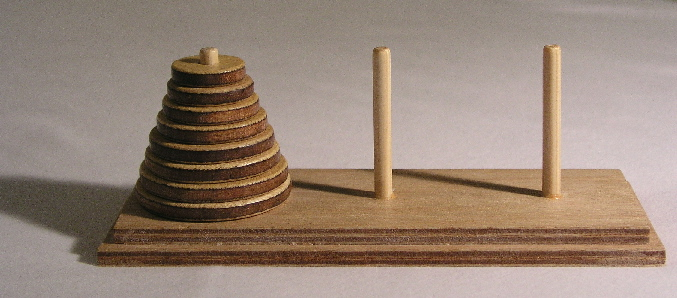
\includegraphics[width=0.5\textwidth]{imagens/torredehanoi.jpg}
 \end{figure}
O objetivo deste jogo é transferir todos os discos de um pino para
outro movendo apenas um disco de cada vez e nunca colocando um disco
maior em cima de um menor.

Apesar de simples, não é óbvio que este quebra-cabeças possui
solução. Após pensar um pouco, podemos perceber que este de fato,
sempre possui solução. Porém, qual será a melhor? Isto é, é possível
solucionar este problema fazendo o menor número de movimentos?

Para chegar a resposta para esta pergunta, devemos primeiro introduzir
algumas notações. Chamaremos de $T(n)$ o número de movimentos
necessários para solucionar o quebra cabeças contendo $n$ discos.

É bastante fácil ver que $T(0) = 0$ e que $T(1) = 1$. A figura
seguinte, mostra passo a passo, a solução para $n = 2$.\\

\begin{figure}[H]
  \centering
      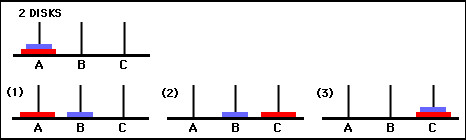
\includegraphics[width=0.5\textwidth]{imagens/hanoi2.jpg}
 \end{figure}

Para $n = 3$, temos: \\

\begin{figure}[h!]
  \centering
      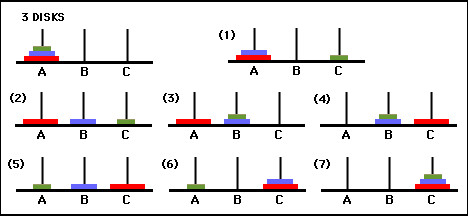
\includegraphics[width=0.5\textwidth]{imagens/hanoi3.jpg}
 \end{figure}

Com isso, temos a seguinte tabela de valores iniciais de $T(n)$:

\[
\begin{array}{|c|c|}
  \hline
  n & T(n)\\ \hline
  0  & 0 \\
  1  & 1 \\
  2 & 3 \\
  3 & 7\\
  \hline
\end{array}
\]

Agora, que fizemos alguns experimentos com este problema, vamos mudar
nossa perspectiva: ao invés de tentar pensar em como resolver este
problema para casos específicos, vamos tentar
generalizá-lo. Observando a figura para a solução com 3 discos,
podemos perceber que o problema para $n = 3$ é resolvido da seguinte
maneira:
\begin{itemize}
  \item Mova $n - 1$ discos do pino $A$ para o pino $B$.
  \item Mova o disco $n$ do pino $A$ para o pino $C$.
  \item Mova $n - 1$ discos do pino $C$ para o pino $C$.
\end{itemize}
Como, para mover $n - 1$ discos de um pino para outro, precisamos de $T(n
-1)$ movimentos, no total precisamos de
\[
T(n - 1) + T(n - 1) + 1 = 2T(n - 1) + 1
\]
para solucionar um quebra-cabeças de tamanho $n$. Assim, temos que o
número mínimo de movimentos para a solução deste problema é dado pela
seguinte função recursiva:
\[
\left\{
\begin{array}{lcl}
T(0) & = & 0 \\
T(n) & = & 2 T(n - 1) + 1
\end{array}
\right.
\]
Mas será que esta função reflete os resultados que obtivemos
solucionando o problema? Vamos fazer os cálculos para $n = 3$:
\[
\begin{array}{lc}
T(3) & = \\
2 T(2) + 1 & = \\
2(2T(1) + 1) + 1 & =\\
2(2(2T(0) + 1) + 1) + 1 & = \\
2(2(2.0 + 1) + 1) + 1 & = \\
7
\end{array}
\]
conforme requerido. Como vimos anteriormente, funções recursivas são
usualmente ineficientes para o cálculo manual. Logo, é uma boa prática
encontrarmos uma fórmula fechada para a função em questão. Porém, já
encontramos esta fórmula no teorema \ref{thmhanoi}.


\subsection{O Problema da Pizzaria}

Suponha que em um fim de semana você tenha ido a uma pizzaria que
possuía a seguinte promoção:

\begin{quote}
``O cliente que conseguir descobrir o número máximo de pedaços que pode
ser obtido ao se fazer $n \in \mathbb{N}$ cortes em uma pizza, não a pagará.''
\end{quote}

Então, como pode-se comer uma pizza de graça? Novamente, vamos seguir
a estratégia utilizada no exemplo anterior. Primeiro, vamos chamar de
$T(n)$ o número de fatias obtidas após fazermos o $n$-ésimo corte. É
bem fácil perceber que $T(0) = 1$, visto que se não fizermos nenhum
corte, temos uma fatia (a pizza inteira). Usando um raciocínio
parecido, temos que $T(1) = 2$, visto que ao fazermos um corte, iremos
dividir a pizza em dois pedaços. Porém, quantos pedaços obtemos ao
fazer o $3^o$ corte? A intuição nos diz que devemos obter $T(3) = 6$,
porém, conforme mostrado na próxima figura, isso não é bem verdade...

\begin{figure}[H]
  \centering
      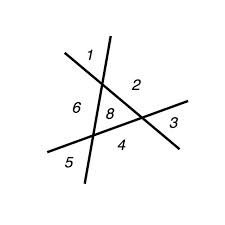
\includegraphics[width=0.5\textwidth]{imagens/plane.jpg}
 \end{figure}

Note que obtemos um número maior de pedaços fazendo com que o
$n$-ésimo corte intercepte todos os cortes anteriores. Com isso,
aumentamos o número total de fatias em $n$ pedaços, isto é, $T(3) = 4
+ 3 = 7$, em que $4 = T(2)$. Desta forma, podemos conjecturar que
$T(n)$ é a seguinte função recursiva:

\[
\left\{
\begin{array}{lcl}
  T(0) & = & 1 \\
  T(n) & = & T(n - 1) + n
\end{array}
\right.
\]

Note que ao calcularmos alguns valores de $T(n)$, podemos notar que
este nada mais é que a soma dos $n$ primeiros números naturais somados
com 1, conforme expandido abaixo:

\[
\begin{array}{lcl}
T(n) & = & T(n - 1) + n \\
       & = & (T(n - 2) + (n - 1)) + n\\
       & = & ( (T(n - 3) + (n - 2)) + (n - 1)) + n\\
       &  & \vdots\\
       & = & T(0) + 1 + 2 + ... + (n -2) + (n - 1) + n\\
       & = & 1 + 1 + 2 + ... + (n -2) + (n - 1) + n\\
       & = & 1 + \sum_{k = 1}^nk
\end{array}
\]
Pode-se mostrar por indução que $\sum_{k = 1}^n =
\frac{n(n+1)}{2}$. Logo, temos que $T(n)$ é dado por:
\[
T(n) = \frac{n(n+1)}{2} + 1
\]
Realmente esta fórmula corresponde a função $T(n)$, conforme provamos
no teorema a seguir.

\begin{Theorem}
Seja $T(n)$ a função definida como:
\[
\left\{
\begin{array}{lcl}
  T(0) & = & 1 \\
  T(n) & = & T(n - 1) + n
\end{array}
\right.
\]
então, $T(n) = \frac{n(n+1)}{2} + 1$.
\end{Theorem}
\begin{proof}
\verb| |\\
\begin{enumerate}
  \item[\ ]Caso base ($n = 0$): Temos que $T(0) = \frac{0(0 + 1)}{2} +
    1$, conforme requerido.
  \item[\ ]Passo indutivo: Suponha $n\in\mathbb{N}$ arbitrário e que
    $T(n) = \frac{n(n+1)}{2} + 1$. Temos que:
   \[
\begin{array}{lcl}
T(n + 1) & = \\
T(n) + (n + 1) & = & \{\text{pela def. de }T(n)\}\\
\dfrac{n(n+1)}{2} + 1 + (n + 1) & = & \{\text{pela hipótese de
  indução}\}\\
\dfrac{n(n + 1) + 2(n+1)}{2}  + 1& = & \\
\dfrac{(n + 1)(n + 2)}{2} + 1
\end{array}
   \]
conforme requerido.
\end{enumerate}
\end{proof}

\subsection{Preenchendo um Tabuleiro de Xadrez}

Considere seguinte quebra-cabeça: preencher um tabuleiro $2^n \times 2^n$, $n
\in \mathbb{N}$, $n\geq 1$, com peças em formato de ``L'' como a
apresentada abaixo:
\begin{figure}[H]
  \centering
      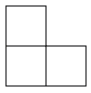
\includegraphics[width=0.15\textwidth]{imagens/tromino.png}
 \end{figure}
de maneira que apenas uma posição do tabuleiro não seja ocupada por
estas peças. Abaixo apresentamos a solução deste quebra-cabeças para
um tabuleiro de $2^3\times 2^3$:
\begin{figure}[H]
  \centering
      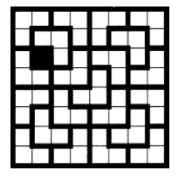
\includegraphics[width=0.35\textwidth]{imagens/tab5.png}
 \end{figure}
em que a posição não ocupada por peças é a que está em ``preto''. A
questão é como resolver este quebra-cabeças para um valor qualquer de
$n \geq 1$?

É fácil ver pela figura abaixo que o quebra-cabeça é obviamente
solúvel para $n = 1$.
\begin{figure}[H]
  \centering
      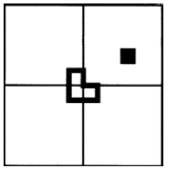
\includegraphics[width=0.35\textwidth]{imagens/tab1.png}
 \end{figure}
Mas, como solucionar este quebra-cabeças para um $n > 1$? O ponto
principal para solucionar este problema para $n > 1$ é observar que um
tabuleiro $2^{n + 1} \times 2^{n + 1}$ é formado por $4$ tabuleiros de
$2^n\times 2^n$. Logo, podemos resolver o quebra-cabeça para um
tabuleiro de $2^{n + 1} \times 2^{n + 1}$ a partir das 4 soluções para
tabuleiros de $2^n\times 2^n$. A chave para combinar as soluções de
cada um dos ``pedaços'' dos quebra cabeças é deixar a posição não
preenchida de cada um destes na extremidade em que esta faz junção
com os outros tabuleiros de mesmo tamanho. Como são 4 tabuleiros de
tamanho $2^n\times 2^n$, haverão 4 posições não preenchidas,
permitindo assim o encaixe de mais uma peça em L, completando a
solução do quebra-cabeça.

A descrição informal acima apresentada, mostra como resolver este
quebra-cabeça, isto é, fornece um algoritmo recursivo para o problema
em questão. Além disso, esta mesma descrição é exatamente a estrutura
de uma prova por indução que mostra que este problema é solúvel para
todo $n \geq 1$. Isto não é uma mera coincidência. Normalmente, provas
por indução possuem a mesma estrutura de algoritmos recursivos.

\begin{Theorem}
Para todo $n \geq 1$, temos que todo tabuleiro de $2^n \times 2^n$
pode ser preenchido por peças em forma de ``L'' de maneira que somente
uma posição do tabuleiro não seja ocupada por uma destas peças.
\end{Theorem}
\begin{proof}
A prova será por indução sobre $n$.
\begin{enumerate}
  \item Caso base ($n = 1$). Imediato. Basta ocupar o tabuleiro com
    uma peça em forma de ``L''.
  \item Passo indutivo. Suponha $n \in \mathbb{N}$ arbitrário e que
    todo tabuleiro de $2^n \times 2^n$ possa ser preenchido de forma que
    apenas uma posição não esteja ocupada. Como um tabuleiro de $2^{n
      + 1} \times 2^{n + 1}$ é formado por 4 tabuleiros de $2^n\times
    2^n$, pela hipótese de indução, estes 4 tabuleiros podem ser
    preenchidos de maneira que uma posição destes não seja
    preenchida. Deixando a posição vazia destes tabuleiros de
    $2^n\times 2^n$ no ponto de junção destes tabuleiros, podemos
    formar a solução para o tabuleiro de $2^{n+1}\times 2^{n+1}$
    acrescentando uma peça, deixando apenas uma posição livre,
    completando assim o quebra-cabeça.
\end{enumerate}
\end{proof}

\section{Exercícios}
\begin{enumerate}
	\item Encontre uma f\'ormula fechada (sem recursividade) equivalente a cada uma das fun\c{c}\~oes recursivas a seguir
		  e prove que a f\'ormula encontrada \'e equivalente a fun\c{c}\~ao em quest\~ao.
	\begin{enumerate}
		\item
				$\left\{
					\begin{array}{l}
						T(0) = 0 \\
						T(n) = 2T(n - 1) + n
					\end{array}
			    \right .$

		\item
				$\left\{
					\begin{array}{l}
						T(0) = 2 \\
						T(n) = (T(n - 1))^{2}
					\end{array}
			    \right .$

		\item
				$\left\{
					\begin{array}{l}
						T(0) = 2 \\
						T(n) = 2T(n - 1) + n
					\end{array}
			    \right .$

		\item
				$\left\{
					\begin{array}{l}
						T(1) = 1 \\
						T(n) = \frac{T(n-1)}{1 + T(n - 1)}
					\end{array}
			    \right .$
               \item
                            $\left\{
					\begin{array}{l}
						T(1) = \frac{1}{4} \\
						T(2) = \frac{1}{8}\\
                                                T(n) =
                                                \frac{T(n-1)T(n-2)}{2T(n-2)
                                                - T(n-1)}
					\end{array}
			    \right .$
	\end{enumerate}
	\item Seja $F(n)$ o $n$-\'esimo termo da sequ\^encia de Fibonacci, definida como:
	\[
		\left\{
			\begin{array}{lcl}
				F(0) & = & 0\\
				F(1) & = & 1 \\
				F(n) & = & F(n - 1) + F(n - 2)
			\end{array}
		\right.
	\]
	Prove os seguintes fatos sobre a sequ\^encia de Fibonacci.
	\begin{enumerate}
		\item $\sum_{i=0}^{n}F(i) = F(n + 2) - 1$
		\item $\sum_{i=0}^{n}F(2i + 1) = F(2n + 2)$
		\item $\sum_{i=0}^{n}(F(i))^{2} = F(n)F(n+1)$
		\item Prove que para todo $n\in\mathbb{N}$, $F(n) < 2^n$.
	\end{enumerate}
        \item Seja $A$ um conjunto. Representamos por
          $\mathcal{P}_{2}(A)$ o conjunto de todos os subconjuntos de
          $A$ que contém $2$ elementos. Prove que para todo conjunto
          $A$, se $|A| = n$, então $|\mathcal{P}_{2}(A)| = \frac{n (n - 1)}{2}$.
\end{enumerate}

\section{Notas Bibliográficas}

Recursividade e sua relação com a indução matemática é um tema
presente em todo texto de matemática discreta. O foco do capítulo
atual foi o uso de indução matemática para demonstrar fórmulas
fechadas equivalentes a funções recursivas. Alguns dos exemplos deste
capítulo foram retirados de \cite{Graham94}.



\appendix
\ifbool{ANSWERS}{
\chapter{Solu\c{c}\~oes para os Exerc\'icios Propostos}

\section{Conceitos Preliminares}

\subsection{1.1.3 Exerc\'icios}

	\begin{enumerate}
	  \item

	  \begin{enumerate}
	    \item
	    \[
	    \begin{array}{ll}
	    & \llbracket \suc (\suc (\suc \zero)) \rrbracket\\
	    = & 1 + \llbracket \suc (\suc (zero)) \rrbracket \\
	    = & 1 + 1 + \llbracket \suc (zero) \rrbracket \\
	    = & 1 + 1 + 1 + \llbracket zero \rrbracket \\
            = & 3
	    \end{array}
	    \]

	    \item
	    \[
	    \begin{array}{llcl}
	    & \length\,(\zero ::\zero :: [\,])& & \\
	    = &1 + \length \,(\zero :: [\,]) & & \{\text{pela equa\c{c}\~ao }(2)\}\\
	    = & 1 + (1 + \length \,[\,])  & & \{\text{pela equa\c{c}\~ao }(2)\}\\
	    = &1 + (1 + 0) & & \{\text{pela equa\c{c}\~ao }(1)\}\\
	    = &2
	    \end{array}
	    \]

	    \item
	    \[
	    \begin{array}{llcl}
	    & (\zero :: (\suc\,\,\zero) :: [\,]) \text{ ++ } ((\suc\,\,\zero) :: \zero :: [\,]) & & \\
	    = & \zero :: (((\suc\,\,\zero) :: [\,]) \text{ ++ } ((\suc\,\,\zero) :: \zero::[\,])) & & \{\text{pela equa\c{c}\~ao }(2)\}\\
	    = & \zero :: ((\suc\,\,\zero) :: ( [\,] \text{ ++ } ((\suc\,\,\zero) :: \zero::[\,]))) & & \{\text{pela equa\c{c}\~ao }(2)\}\\
	    = & \zero :: ((\suc\,\,\zero) :: ((\suc\,\,\zero) :: \zero::[\,])) & & \{\text{pela equa\c{c}\~ao }(1)\}\\
	    \end{array}
	    \]
	  \end{enumerate}

	  \item  A defini\c{c}\~ao de concatena\c{c}\~ao de listas \'e uma fun\c{c}\~ao pois satisfaz os crit\'erios de totalidade e termina\c{c}\~ao, isso se dá devido ao fato de que, pelas regras $(1) \, e \, (2)$ definimos a sem\^antica recursivamente sobre a primeira lista cobrindo todas as possibilidades de constru\c{c}\~oes dos termos da sintaxe(sejam elas uma lista vazia ou uma lista n\~ao vazia), e tamb\'em porque a defini\c{c}\~ao e aplicada recursivamente sobre os subtermos da primeira lista e tendo como caso base a regra $(1)$\,.

	  \item
	  \[
	  \begin{array}{lcl}
	  \textit{nsubtermos } (\tconst\, n)  & = & 1 \\
	  \textit{nsubtermos } (\tplus\,e_1\,e_2) & = & 1 +
          (\textit{nsubtermos }\,e_1) + (\textit{nsubtermos }\,e_2) \\
	  \textit{nsubtermos }(\ttimes\,e_1\,e_2) & = & 1
          + (\textit{nsubtermos }\,e_1) + (\textit{nsubtermos }\,e_2) \\
	  \end{array}
	  \]

	  Temos a definição de uma função que retorna a quantidade de subtermos de uma expressão arimética de linguagem $\TExp$. Isso porque pelo princípio da totalidade a definição abrange todo possível valor de entrada na função, seja ele $(\tconst\, n)$, $(\tplus\,e_1\,e_2)$, $(\ttimes\,e_1\,e_2)$ e pelo principio da terminação a cada chamada recursiva da função o número de subtermos diminui tendendo a chegar no caso base que teria como entrada uma constante do tipo $(\tconst\, n)$


	  \item
	  \begin{enumerate}
	  \item Caso a definição de concatenação de listas fosse apresentada somente com a seguinte regra:
	  	  \[
	  	  \begin{array}{c}
	  	  	(x :: xs) \text{ ++ }  ys  =  x :: (xs\text{ ++ } ys)
	  	  \end{array}
	  	  \]
	  não poderíamos chamá-la de função devido ao fato de que esta definição não segue o princípio da totalidade, uma vez que não há procedimento para o caso de lista vazia.

	 \item Tomando o caso dos números naturais como base, não poderíamos criar uma função semântica somente com a seguinte regra:
	 	 \[
	 	 \begin{array}{c}
	 	 	\llbracket \suc\,\,n\rrbracket  =  \llbracket \suc\,n \rrbracket + 1
	 	\end{array}
	 	\]
	 já que ela não segue o principio da terminação sendo que a
         cada chamada recursiva é feita sobre um termo que não é menor
         que o parâmetro original de entrada.
	 \end{enumerate}

	\end{enumerate}

\ifbool{COQ}{
\subsection{1.2.3 Exerc\'icios}

	\begin{enumerate}
		\item

		\begin{lstlisting}
		Fixpoint evalExp (e: Exp) : nat :=
	     match e with
	      | Const n => NatSem n
	      | Plus (h)(t) => (evalExp h) + (evalExp t)
	      | Times (h)(t)=> (evalExp h) * (evalExp t)
	    end.
	    \end{lstlisting}
		Note que para esta fun\c{c}\~ao funcionar, se faz necess\'ario a declara\c{c}\~ao das seguintes defini\c{c}\~oes antes do corpo da fun\c{c}\~ao em quest\~ao.

		\begin{lstlisting}
		Inductive Nat : Set :=
		  | Zero : Nat
		  | Succ : Nat -> Nat.
		\end{lstlisting}

		\begin{lstlisting}
		Inductive Exp : Set :=
		  | Const : Nat -> Exp
		  | Plus : Exp -> Exp -> Exp
		  | Times : Exp -> Exp -> Exp .
		\end{lstlisting}

		\begin{lstlisting}
		Fixpoint NatSem (n : Nat) : nat :=
			match n with
			| Zero  => 0
			| Suc n' => 1 + NatSem n'
		end.
		\end{lstlisting}


		\item
		\begin{lstlisting}
		Inductive List (T : Set ) : Set :=
	 	  | nil : List T
		  | cons : T -> List T -> List T.
		\end{lstlisting}

		\begin{lstlisting}
		Definition tail {T} (l : List T) : List T :=
		  match l with
		  | nil => l
		  | cons h t => t
		  end.
		\end{lstlisting}

		\item

		\begin{lstlisting}
		Inductive List (T : Set ) : Set :=
		  | nil : List T
		  | cons : T -> List T -> List T.
		\end{lstlisting}


		\begin{lstlisting}
		Fixpoint last {T} (default : T) (l : List T) : T :=
		  match l with
		  | nil => default
		  | cons h t => last t
		  | cons t nil => t
		  end.
		\end{lstlisting}

	\end{enumerate}
}{}
\section{L\'ogica Proposicional}

\subsection{2.2.1 Exerc\'icios}

	\begin{enumerate}
		\item 
			\begin{enumerate}
				\item
				 \[\begin{array}{ll}    
				 \text{Jo\~ao \'e pol\'itico} & \text{Conjun\c{c}\~ao (mas) }\\
				 \text{Jo\~ao \'e honesto} & \\
				 \end{array}
				 \]
				 
				 \item
				 \[\begin{array}{ll}    
 				 \text{Jo\~ao \'e honesto} & \text{Conjun\c{c}\~ao (mas), Nega\c{c}\~ao (n\~ao) }\\
 				 \text{O irm\~ao de Jo\~ao \'e honesto} & \\
 				 \end{array}
 				 \]
 				 
 				 \item
 				 \[\begin{array}{ll}    
  				 \text{Jo\~ao vir\'a a festa} & \text{Disjun\c{c}\~ao (ou), Conjun\c{c}\~ao (al\'em) }\\
  				 \text{A irm\~a de Jo\~ao vir\'a a festa.} & \\
  				 \text{A m\~ae de Jo\~ao vir\'a a festa.} & \\
  				 \end{array}
  				 \]
				 
				 \item
  				 \[\begin{array}{ll}    
   				 \text{A estrela do espet\'aculo canta.} & \text{Nega\c{c}\~ao (n\~ao) , Conjun\c{c}\~ao + Nega\c{c}\~ao (nem)} \\
   				 \text{A estrela do espet\'aculo dan\c{c}a.} & \\
   				 \text{A estrela do espet\'aculo representa.} & \\
   				 \end{array}
   				 \]
				 
				 \item
   				 \[\begin{array}{ll}    
  				 \text{O trem apita.} & \text{Condicional (Sempre que \ldots) } \\
  				 \text{Jo\~ao sai correndo.} & \\
  				 \end{array}
  				 \]
				 
				 \item
    			 \[\begin{array}{ll}    
   				 \text{Jo\~ao perde dinheiro no jogo.} & \text{Condicional (Caso \ldots), Nega\c{c}\~ao (n\~ao) } \\
   				 \text{Jo\~ao vai a festa.} & \\
   				 \end{array}
   				 \]
				  
				 \item
     			 \[\begin{array}{ll}    
  				 \text{Jo\~ao vai ser multado.} & \text{Condicional (a menos que \ldots) }  \\
  				 \text{Jo\~ao diminui a velocidade.} & \text{Disjun\c{c}\~ao (ou), Nega\c{c}\~ao (n\~ao)} \\
  				 \text{A rodovia tem radar.} & \\
  				 \end{array}
  				 \]
				 				  
				\item
   			    \[\begin{array}{ll}    
				\text{Um n\'umero natural \'e primo.} & \text{Condicional (Uma condi\c{c}\~ao suficiente \ldots)} \\
				\text{Um n\'umero natural \'e \'impar.} & \\
				\end{array}
				\]
				 
				\item
			    \[\begin{array}{ll}    
				\text{Jo\~ao vai ao teatro.} & \text{Condicional (somente se \ldots)} \\
				\text{Uma com\'edia est\'a em cartaz.} & \\
				\end{array}
				\]
				  
				\item
			    \[\begin{array}{ll}    
				\text{Voc\^e \'e Brasileiro.} & \text{Condicional   (Se\ldots)} \\
				\text{Voc\^e gosta de futebol.} & \text{Bicondicional + Nega\c{c}\~ao (a menos \ldots)} \\
				\text{Voc\^e tor\c{c}e para o Tabajara.} & \\
				\text{Voc\^e tor\c{c}e para o \'Ibis.} & \\
				\end{array}
				\]  
				
				\item
			    \[\begin{array}{ll}    
				\text{A propina ser\'a paga.} & \text{Bicondicional (exatamente nas situa\c{c}\~oes} \\
				\text{O deputado vota como instru\'ido por Jo\~ao.} & \text{ em que \ldots)} \\
				\end{array}
				\]
	 
			\end{enumerate}

	\end{enumerate}


\subsection{2.2.3 Exerc\'icios}
	
		\begin{enumerate}
			\item
			\begin{enumerate}
							
			\item  $(A \lor B) \to C$
			\[\begin{array}{c|l} 		
			\text{Vari\'avel} & \text{Proposi\c{c}\~ao Simples} \\ \hline
   			$A$        & \text{Jane vence}\\ 
   			$B$        & \text{Jane perde}\\
   			$C$        & \text{Jane fica cansada} \\									
			\end{array}
			\]			
										
			\item  $A \lor B$
			\[\begin{array}{c|l} 		
			\text{Vari\'avel} & \text{Proposi\c{c}\~ao Simples} \\ \hline
   			$A$        & \text{Rosas s\~ao vermelhas}\\ 
   			$B$        & \text{Violetas s\~ao azuis}\\											
			\end{array}
			\]
		
			\item  $A \to B$
			\[\begin{array}{c|l} 
			\text{Vari\'avel} & \text{Proposi\c{c}\~ao Simples} \\ \hline
			$A$        & \text{Elefantes podem subir em \'arvores}\\ 
			$B$        & \text{3 \'e um n\'umero irracional}\\
			\end{array}
			\]
					
			\item $A \lor B$
			\[\begin{array}{c|l} 
			\text{Vari\'avel} & \text{Proposi\c{c}\~ao Simples} \\ \hline
			$A$        & \text{\'E proibido fumar cigarros}\\ 
			$B$        & \text{3 \'e um n\'umero irracional}\\
			\end{array}
			\]												
			
			\item $ \neg \,(A \to B )$
			\[\begin{array}{c|l} 
			\text{Vari\'avel} & \text{Proposi\c{c}\~ao Simples} \\ \hline
			$A$        & \pi > 0\\ 
			$B$        & \pi > 1\\
			\end{array}
			\]
			
			\item $ A \to B $
			\[\begin{array}{c|l} 
			\text{Vari\'avel} & \text{Proposi\c{c}\~ao Simples} \\ \hline
			$A$        & \text{As laranjas s\~ao amarelas}\\ 
			$B$        & \text{Os morangos s\~ao vermelhos}\\
			\end{array}
			\]			
						
			\item $ \neg ( A \to B) $
			\[\begin{array}{c|l} 
			\text{Vari\'avel} & \text{Proposi\c{c}\~ao Simples} \\ \hline
			$A$        & \text{Montreal \'e a capital do Canad\'a}\\ 
			$B$        & \text{A pr\'oxima copa ser\'a realizada no Brasil}\\
			\end{array}
			\]
	
			\end{enumerate}
	

	
			\item
				\begin{enumerate}
				
				\item $ A \land B $
				\[\begin{array}{c|l} 
				\text{Vari\'avel} & \text{Proposi\c{c}\~ao Simples} \\ \hline
				$A$        & \text{Jo\~ao \'e pol\'itico}\\ 
				$B$        & \text{Jo\~ao \'e honesto}\\
				\end{array}
				\]
					
				\item $ A \land \neg B $
				\[\begin{array}{c|l} 
				\text{Vari\'avel} & \text{Proposi\c{c}\~ao Simples} \\ \hline
				$A$        & \text{Jo\~ao \'e honesto}\\ 
				$B$        & \text{O irm\~ao de jo\~ao \'e honesto}\\
				\end{array}
				\]

				\item $ (A \lor B ) \land C $
				\[\begin{array}{c|l} 
				\text{Vari\'avel} & \text{Proposi\c{c}\~ao Simples} \\ \hline
				$A$        & \text{Jo\~ao vir\'a a festa}\\ 
				$B$        & \text{A irm\~a de Jo\~ao vir\'a a festa}\\
				$C$ 	   & \text{A m\~ae de Jo\~ao vir\'a a festa} \\
				\end{array}
				\]
				
				\item $ \neg A \land \neg B \land \neg C $
				\[\begin{array}{c|l} 
				\text{Vari\'avel} & \text{Proposi\c{c}\~ao Simples} \\ \hline
				$A$        & \text{A estrela do espet\'aculo canta}\\ 
				$B$        & \text{A estrela do espet\'aculo dan\c{c}a}\\
				$C$ 	   & \text{A estrela do espet\'aculo representa} \\
				\end{array}
				\]
				
				\item $ A \to B $
				\[\begin{array}{c|l} 
				\text{Vari\'avel} & \text{Proposi\c{c}\~ao Simples} \\ \hline
				$A$        & \text{O trem apita}\\ 
				$B$        & \text{Jo\~ao sai correndo}\\
				\end{array}
				\]
 
				\item $ \neg A \to B $
				\[\begin{array}{c|l} 
				\text{Vari\'avel} & \text{Proposi\c{c}\~ao Simples} \\ \hline
				$A$        & \text{Jo\~ao perde dinheiro no jogo}\\ 
				$B$        & \text{Jo\~ao vai a festa}\\
				\end{array}
				\] 
				
				\item $ A \to \neg (B \lor \neg C) $
				\[\begin{array}{c|l} 
				\text{Vari\'avel} & \text{Proposi\c{c}\~ao Simples} \\ \hline
				$A$        & \text{Jo\~ao vai ser multado}\\ 
				$B$        & \text{Jo\~ao diminui a velocidade}\\
				$C$        & \text{A rodovia tem radar}\\
				\end{array}
				\]
				
				\item $ A \to B $
				\[\begin{array}{c|l} 
				\text{Vari\'avel} & \text{Proposi\c{c}\~ao Simples} \\ \hline
				$A$        & \text{Um n\'umero natural \'e primo}\\ 
				$B$        & \text{Um n\'umero natural \'e \'impar}\\
				\end{array}
				\]		
						
				\item $ A \to B $
				\[\begin{array}{c|l} 
				\text{Vari\'avel} & \text{Proposi\c{c}\~ao Simples} \\ \hline
				$A$        & \text{Jo\~ao vai ao teatro}\\ 
				$B$        & \text{Uma com\'edia est\'a em cartaz}\\
				\end{array}
				\]		
									
				\item $ (A \to B) \to \neg (C \lor D) $
				\[\begin{array}{c|l} 
				\text{Vari\'avel} & \text{Proposi\c{c}\~ao Simples} \\ \hline
				$A$        & \text{Voc\^e \'e Brasileiro}\\ 
				$B$        & \text{Voc\^e gosta de futebol}\\
				$C$        & \text{Voc\^e tor\c{c}e para o Tabajara}\\ 
				$D$        & \text{Voc\^e tor\c{c}e para o \'Ibis}\\
				\end{array}
				\]		
								
				\item $ A \leftrightarrow B $
				\[\begin{array}{c|l} 
				\text{Vari\'avel} & \text{Proposi\c{c}\~ao Simples} \\ \hline
				$A$        & \text{A propina ser\'a paga}\\ 
				$B$        & \text{O deputado vota como instru\'ido por Jo\~ao}\\
				\end{array}
				\]		
							
				\end{enumerate}
	
		\end{enumerate}

\subsection{2.3.1 Exerc\'icios}

	\begin{enumerate}
	
			\item 
			\begin{enumerate}		
					\item 
					Pela regra 2 temos que as vari\'aveis $A$, $B$ e $C$ s\~ao f\'ormulas da l\'ogica, com isso pela regra 3\,-a temos que $\neg A$ tamb\'em faz parte do conjunto de f\'ormulas. Pela regra 3\,-b temos $\neg A \land B$. Novamente por 3\,-b podemos concluir $\neg A \land B \to C $. 
					
					\item
					Pela regra 2 temos que as vari\'aveis $A$, $B$ e $C$ s\~ao f\'ormulas da l\'ogica. Por 3\,-b temos $A \to B$ e $A \lor B$, com isso, novamente por 3\,-b conclu\'imos $A \lor B \to C$. Pela regra 3\,-a temos $\neg(A \lor B \to C)$ e por fim, pela regra 3\,b chegamos a $(A \to B) \land \neg(A \lor B \to C)$.
					
					\item
					Pelas regras 1 e 2 temos que as vari\'aveis $A$, $B$, $C$ e a constante $ \bot $ pertence ao conjunto de f\'ormulas da l\'ogica. Tomando como base a regra 3\,-b temos $B \to C$ que por sua vez podemos concluir $A \to B \to C $ e novamente por 3\,-b conclu\'imos  $A \to B \to C \leftrightarrow \bot $.
					
					\item
					Pela regra 2 temos que as vari\'aveis $A$, $B$ s\~ao f\'ormulas da l\'ogica, com isso pela regra 3\,-a temos que $\neg A$ tamb\'em faz parte do conjunto de f\'ormulas. Por 3\,-b pode-se construir $\neg A \to B $, novamente por 3\,-b $ A \land \neg A \to B $.
					
					\item
					Pela regra 2 temos que as vari\'aveis $A$, $B$ e $C$ s\~ao f\'ormulas da l\'ogica. Por 3\,-b temos $B \land C$ e com isso conclu\'imos $A \lor B \land C$.			
			\end{enumerate}
			
			\item
			\begin{enumerate}
				\item $(\neg A \land B) \to C$
				\item $(A \to B) \land \neg((A \lor B) \to C)$
				\item $(A \to (B \to C)) \leftrightarrow \bot$
				\item $(A \land \neg A) \to B$
				\item $A \lor (B \land C)$
			\end{enumerate}
			
			
			\item
			\begin{enumerate}
				\item $(A \lor B) \lor (C \lor D)$
				\item $A \to B \to (A \land B)$
				\item $\neg (A \lor B \land C)$
				\item $\neg (A \land (B \lor C))$
			\end{enumerate}
	
	\end{enumerate}

\subsection{2.4.10 Exerc\'icios}


	\begin{enumerate}
	
	
			\item
			\begin{enumerate}
			
			%LETRA A -------------------------------------------->
			\item Conting\^encia	
			\[\begin{array}{|c|c|c|c|c|c|}
			\hline
			 A & B & A \to B & A \lor B & \neg(A \lor B)& (A \to B) \leftrightarrow \neg(A \lor B) \\ \hline
			T & T & T & T & F & F \\
			T & F & F & T & F & F \\
			F & T & T & T & F & F \\
			F & F & T & F & T & T \\
			\hline
			\end{array}
			\]	
			
			
			%LETRA B -------------------------------------------->
			\item Conting\^encia		
			\[\begin{array}{|c|c|c|c|c|c|}
			\hline
			A & B & C & A \land B & (A \land B) \lor C & B \lor C \\ \hline
			T & T & T & T & T & T \\
			T & T & F & T & T & T \\
			T & F & T & F & T & T \\
			T & F & F & F & F & F \\
			F & T & T & F & T & T \\
			F & T & F & F & F & T \\
			F & F & T & F & T & T \\
			F & F & F & F & F & F \\
			\hline
			\end{array}
			\]
			
			\[\begin{array}{|c|c|}
			\hline
			A \land (B \lor C) & (A \land B) \lor C \to A \land (B \lor C)  \\ \hline
			T & T \\
			T & T \\
			T & T \\
			F & T \\
			F & F \\
			F & T \\
			F & F \\
			F & T \\
			\hline
			\end{array}
			\]
			
			%------------------------------------------------------>
			
		
			%LETRA C -------------------------------------------->
			\item Conting\^encia		
			\[\begin{array}{|c|c|c|c|c|}
			\hline
			A & B & \neg A & \neg B & \neg A \lor \neg B \\ \hline
			T & T & F & F & F \\
			T & F & F & T & T \\
			F & T & T & F & T \\
			F & F & T & T & T \\
			\hline
			\end{array}
			\]
			
			
			\[\begin{array}{|c|c|}
			\hline
			\neg(\neg A \lor \neg B) & A \land \neg(\neg A \lor \neg B) \\ \hline
			T & T \\
			F & F \\
			F & F \\
			F & F \\
			\hline
			\end{array}
			\]
			%------------------------------------------------------>
						
					
			%LETRA D -------------------------------------------->
			\item Conting\^encia
			\[\begin{array}{|c|c|c|c|c|}
			\hline
			A & B & A \land B & \neg A & A \land B \to \neg A \\ \hline
			T & T & T & F & F\\
			T & F & F & F & T\\
			F & T & F & T & T\\
			F & F & F & T & T\\
			\hline
			\end{array}
			\]
			
			
			%LETRA E -------------------------------------------->
			\item Tautologia
			\[\begin{array}{|c|c|c|c|c|c|}
			\hline
			A & B & C & A \to B & A \lor C & B \lor C \\ \hline
			T & T & T & T & T & T \\
			T & T & F & T & T & T \\
			T & F & T & F & T & T \\
			T & F & F & F & T & F \\
			F & T & T & T & T & T \\
			F & T & F & T & F & T \\
			F & F & T & T & T & T \\
			F & F & F & T & F & F \\
			\hline
			\end{array}
			\]
			
			\[\begin{array}{|c|c|}
			\hline
			(A \lor C) \to (B \lor C) & (A \to B) \to [(A \lor C) \to (B \lor C)] \\ \hline
			T & T \\
			T & T \\
			T & T \\
			F & T \\
			T & T \\
			T & T \\
			T & T \\
			T & T \\
			\hline
			\end{array}
			\]
			%------------------------------------------------------>
			
			%LETRA F -------------------------------------------->
			\item Tautologia
			\[\begin{array}{|c|c|c|c|}
			\hline
			A & B & B \to A & A \to (B \to A) \\ \hline
			T & T & T & T \\
			T & F & T & T \\
			F & T & F & T \\
			F & F & F & T \\
			\hline
			\end{array}
			\]
			
			%LETRA G -------------------------------------------->
			\item Contradi\c{c}\~ao
			\[\begin{array}{|c|c|c|c|c|}
			\hline
			A & B & A \land B & \neg B & \neg A \\ \hline
			T & T & T & F & F \\
			T & F & F & T & F \\
			F & T & F & F & T \\
			F & F & F & T & T \\
			\hline
			\end{array}
			\]
			
			\[\begin{array}{|c|c|}
			\hline
			(\neg B \lor \neg A) & (A \land B) \leftrightarrow (\neg B \lor \neg A) \\ \hline
			F & F \\
			T & F \\
			T & F \\
			T & F \\
			\hline
			\end{array}
			\]
			
			%------------------------------------------------------>			
			\end{enumerate}
			
			\item
			\begin{enumerate}
				
				%2a
				\item 
				\[\begin{array}{|c|c|c|c|}
				\hline
				P & Q & P \leftrightarrow Q & P \to Q \\ \hline
				T & T & T & T \\
				T & F & F & F \\
				F & T & F & T \\
				F & F & T & T \\
				\hline
				\end{array}
				\]
				
				\[\begin{array}{|c|c|c|c|}
				\hline
				\neg P & \neg Q & (\neg P \to \neg Q) & (P \to Q) \land (\neg P \to \neg Q) \\ \hline
				F & F & T & T \\
				F & T & T & T \\
				T & F & F & F \\
				T & T & T & T \\
				\hline
				\end{array}
				\]
				
				Pela an\'alise das tabelas anteriores podemos concluir que  $P \leftrightarrow Q$ e $(P \to Q) \land (\neg P \to \neg Q)$ n\~ao s\~ao f\'ormulas equivalentes da l\'ogica proposicional, pois apresentam resultados diferentes na solu\c{c}\~ao da tabela verdade.
				
				\item
				\[\begin{array}{|c|c|c|c|c|c|c|}
				\hline
				P & Q & \neg P & \neg Q & P \land \neg Q & \neg P \land Q & (P \land \neg Q) \lor (\neg P \land Q) \\ \hline
				T & T & F & F & F & F & F \\
				T & F & F & T & T & F & T \\
				F & T & T & F & F & T & T \\
				F & F & T & T & F & F & F \\
				
				
				\hline
				\end{array}
				\]
				
				\[\begin{array}{|c|c|c|c|}
				\hline
				P \lor Q & P \land Q & \neg (P \land Q)& (P \lor Q) \land \neg (P \land Q) \\ \hline
				T & T & F & F \\
				T & F & T & T \\
				T & F & T & T \\
				F & F & T & F \\
				\hline
				\end{array}
				\]
				
				$(P \land \neg Q) \lor (\neg P \land Q)$ e $(P \lor Q) \land \neg (P \land Q)$ s\~ao f\'ormulas equivalentes da l\'ogica proposicional, j\'a que apresentam resultados iguais pela tabela verdade.		
			\end{enumerate}
			
			\item 
			\begin{enumerate}
				
				\item Quando dizemos que uma f\'ormula e satisfaz\'ivel isso indica que pelo menos um resultado do conjunto de valores poss\'iveis daquela f\'ormula \'e verdadeiro. Supondo que a f\'ormula a ser analisada seja uma tautologia, a nega\c{c}\~ao da mesma nos dar\'a uma contradi\c{c}\~ao. Portanto se passarmos a nega\c{c}\~ao da f\'ormula para o algoritmo e este retornar falso conclu\'imos que a nega\c{c}\~ao n\~ao \'e satisfaz\'ivel e portanto uma contradi\c{c}\~ao, o que confirma a nossa hip\'otese de que a f\'ormula \'e uma tautologia.
				
				\item Se passarmos a f\'ormula para o algoritmo e este nos retornar falso indica que a f\'ormula n\~ao \'e satisfaz\'ivel e portanto n\~ao possui nenhum resultado no conjunto de valores poss\'iveis com o valor verdadeiro, com isso temos a defini\c{c}\~ao de contradi\c{c}\~ao.
				
			\end{enumerate}
			
			
	\end{enumerate}
	
\subsection{2.5.7 Exerc\'icios}
\begin{enumerate}
	\item
	\begin{enumerate}
	\item $\{(P\land Q)\land R,\, S\land T\}\vdash\,Q\land S$
	
	\[
      \infer[\andI]
               {Q\land S}
               {
                   \infer[\andED]
                            {Q}
                            {
                            \infer[\andEE]
                            		{P\land Q}
                            		{
                            			\infer[\Id]
                            				{(P\land Q)\land R}
                            				{}
                            		}
                            }
                    &  
                   \infer[\andEE]
                            {S}
                            {
	                            \infer[\Id]
	                                   {S\land T}{}
                            }
               }
 	 \]
 	 
 	 
 	 \item $\{(P\land Q)\land R\}\,\vdash\,(P\land R)\lor Z$
 	 
 	 \[
 	 	\infer[\orIE]
 	 		{(P\land R)\lor Z}
 	 		{
 	 			\infer[\andI]
 	 				{P \land R}
 	 				{
 	 					\infer[\andEE]
 	 						{P}
 	 						{
 	 							\infer[\andEE]
 	 								{P\land Q}
 	 								{\infer[\Id]{(P\land Q)\land R}{}}
 	 						}
 	 					&
 	 					\infer[\andED]
 	 						{R}
 	 						{\infer[\Id]{(P\land Q)\land R}{}}
 	 				}
 	 		}
 	 \]
 	 
 	 \item  $\{Q\rightarrow (P\rightarrow R),\, \neg R,\, Q\,\} \vdash\,\neg P$
		
	\[
		\infer[\Id]
			{\neg P}
			{
				\infer[\impI^1]
					{P \to \bot}
					{
						\infer[\impE]
							{\bot}
							{
								\infer[\Id]
									{R \to \bot}{}
							&
								\infer[\impE]
									{R}
									{
										\infer[\impI]
											{P \to R}
											{
												\infer[\Id]
													{Q \to (P \to R)}
													{}
												&
												\infer[\Id]
													{Q}
													{}
											}
										&
										\infer[\Id]
											{P^1}
											{}
									}
							}
					}
			}	
	\]
	
	\item $\{P\}\,\vdash\, Q\rightarrow(P\land Q)$
	
	\[
		\infer[\impI^1]
			{Q\rightarrow(P\land Q)}
			{
				\infer[\andI]
					{P\land Q}
					{
						\infer[\Id]
							{P}
							{}
						&
						\infer[\Id]
							{Q^1}
							{}
					}
			}
	\]
	
	\item $\{(P\rightarrow R)\land (Q\rightarrow R),\, P\land Q\}\,\vdash\, Q\land R$
	
	\[
		\infer[\andI]
			{Q\land R}
			{
				\infer[\andED]
					{Q}
					{
						\infer[Id]
							{P \land Q}
							{}
					}
				&
				\infer[\impE]
					{R}
					{
						\infer[\andEE]
							{P \to R}
							{
								\infer[Id]
									{(P \to R)\land(Q \to R)}
									{}
							}
						&
						\infer[\andEE]
							{P}
							{
								\infer[Id]
									{P \land Q}
									{}
							}
					}
			}
	\]
	
	\item $\{P\rightarrow Q, R\rightarrow S\}\vdash (P\lor R)\rightarrow (Q\lor S)$
	
	\[
		\infer[\impI^1]
			{(P \lor R) \to (Q \lor S)}
			{
				\infer[\orE]
					{Q \lor S}
					{
						\infer[Id]
							{P \lor R}
							{} &
						\infer[\orIE]
							{Q \lor S }
							{
								\infer[\impE]
									{Q}
									{
										\infer[Id]
											{P \to Q}
											{}
										&
										P^1
									}
							} &
						\infer[\orID]
							{Q \lor S }
							{
								\infer[\impE]
									{S}
									{
										\infer[Id]
											{R \to S}
											{}
										&
										R^1
									}
							}
					}
			}
	\]
	\item $\{Q\rightarrow R\}\vdash (P\rightarrow Q)\rightarrow(P\rightarrow R)$
	\[
		\infer[\impI^1]
			{(P \to Q) \to (P \to R)}
			{
				\infer[\impI^2]
					{P \to Q}
					{
						\infer[\impE]
						{Q}
						{
							\infer[\Id]
								{Q \to R}
								{}
							&
							\infer[\impE]
								{Q}
								{
									\infer[\Id^1]
										{P \to Q}
										{}
									&
									\infer[\Id^2]
										{P}
										{}
								}
						}
					}
			}	
	\]
	
	\item $\{(P\land Q)\lor(P\land R)\}\vdash P\land(Q \lor R)$ 
	\[
     	\infer[\orE^1]
              {P \land (Q \lor R)}
              {
                (P\land Q)\lor(P\land R) 
                &
                \infer[\andI]
                         {P\land (Q \lor R)}
                         {
                           \infer[\andEE]
                                    {P}
                                    {P \land Q^1}
                            &
                            \infer[\orIE]
                                     {Q \lor R}
                                     {
                                         \infer[\andED]
                                                  {Q}
                                                  {P \land Q^1}
                                     } 
                         }
                 &
                \infer[\andI]
                         {P \land (Q \lor R)}
                         {
                           \infer[\andED]
                                    {P}
                                    {P \land R^1}
                            &
                            \infer[\orIE]
                                     {Q \lor R}
                                     {
                                         \infer[\andED]
                                                  {R}
                                                  {P \land R^1}
                                     }
                         }
              }
     \]

	\item $\{\neg(A \lor B)\}\vdash \neg A \land \neg B$
	
	\[
		\infer[\andI]
			{\neg A \land \neg B}
			{
			 \infer[\Id]
			 	{\neg A}
			 	{
			 		\infer[\impI^1]
			 			{A \to \bot}
			 			{
			 				\infer[\impE]
			 					{\bot}
			 					{
			 						\infer[\Id]
			 							{(A \lor B) \to \bot}
			 							{\neg(A \lor B)}
			 					&
			 						\infer[\orIE]
			 							{A \lor B}
			 							{A^1}
			 					}
			 			}
			 	}
				&
			 \infer[\Id]
			 	{\neg B}
			 	{
			 		\infer[\impI^2]
			 			{B \to \bot}
			 			{
			 				\infer[\Id]
			 					{(A \lor B) \to \bot}
			 					{\neg(A \lor B)}
			 			&
			 				\infer[\orID]
			 					{A \lor B}
			 					{B^2}
			 			}
			 	}
			}
	\]
	
	\item $\{\neg A \land \neg B\}\vdash \neg (A\lor B)$
	
	\[
		\infer[\Id]
			{\neg (A\lor B)}
			{
				\infer[\impI^1]
					{(A \lor B) \to \bot}
					{
						\infer[\impE]
							{\bot}
							{
								\infer[\Id]
									{\neg(A \lor B)}
									{\neg A \land \neg B}
								&
								(A \lor B)^1	
							}
					}
			}
	\]
	
	\item $\{\neg(A \land B)\}\vdash \neg A \lor \neg B$ 
	\paragraph*{Obs.:}Note que n\~ao \'e poss\'ivel resolver este exerc\'icio sem o uso da t\'ecnica de Redu\c{c}\~ao do Absurdo.
	\[
		\infer[\raa^1]
			{\neg A \lor \neg B}
			{
				\infer[\impE]
					{\bot}
					{
					\infer[\Id]
						{\neg(A \land B)}
						{}
					 &	
					 \infer[\andI]
					 	{A \land B}
					 	{
					 		\infer[\raa^2]
					 			{A}
					 			{
					 				\infer[\impE]
					 					{\bot}
					 					{
					 						\neg(\neg A \lor \neg B)^1
					 						&
					 						\infer[\orIE]
					 							{\neg A \lor \neg B}
					 							{
					 							 \neg A^2
					 							}
					 					}
					 			}
					 		&
					 		\infer[\raa^3]
					 			{B}
					 			{
					 				\infer[\impE]
					 					{\bot}
					 					{			 						\neg(\neg A \lor \neg B)^1
											&   						\infer[\orIE]						{\neg A \lor \neg B}												 										 																		 {\neg B^3}	
						 			}
					 			}	
					 	}
					}
			}
	\]
	
	

	\item $\{\neg A \lor \neg B\}\vdash \neg (A\land B)$
	
	\[
		\infer[\Id]
			{\neg (A \land B)}
			{
				\infer[\impI^1]
					{(A \land B) \to \bot}	
					{
						\infer[\orE^2]
							{\bot}
							{
								\neg A \lor \neg B
								&
									\infer[\impE]
										{\bot}
										{
											\infer[\Id]
												{A \to \bot}
												{\neg A^2}
										&
											\infer[\andEE]
												{A}
												{(A \land B)^1}
										}
								&
									\infer[\impE]
										{\bot}
										{
											\infer[\Id]
												{B \to \bot}
												{\neg B^2}
										&
											\infer[\andED]
												{B}
												{(A \land B)^1}
										}
							}
					}
			}
	\]
	\end{enumerate}
	
	\item
	\begin{enumerate}
		\item $\{A \to B\}\vdash \neg A \lor B$
			\[
				\infer[\raa^1]
					{\neg A \lor B}
					{
						\infer[\impE]
							{\bot}
							{
								\infer[\andED]
									{\neg B}
									{A \land \neg B^1}
								&
								\infer[\impE]
									{B}
									{
										\infer[\Id]
											{A \to B}
											{}
										&
										\infer[\andEE]
											{A}
											{A \land \neg B^1}
									}	
							}	
					}		
			\]
		\item $\vdash (\neg B \to \neg A)\to (A \to B)$
			\[
				\infer[\impE^1]
					{(\neg B \to \neg A)\to (A \to B)}
					{
						\infer[\impE^2]
							{A \to B}
							{
								\infer[\raa^3]
									{B}
									{
										\infer[\impE]
											{\bot}
											{
												\infer[\Id]
													{A \to \bot}
													{
														\infer[\impE]
															{\neg A}
															{
																(\neg B \to \neg A)^1
																&
																\neg B^3	
															}
													}
												&
												A^2
											}
									}
							}
					}
			\]
		
		\item Em andamento
		\item Em andamento

	\end{enumerate}
	
\end{enumerate}

\subsection{2.6.6 Exerc\'icios}

\begin{enumerate}
	\item
	\begin{enumerate}
		
			\item $(A\lor B)\land B\equiv B$
			\[
				\begin{array}{lcl}
					(A \lor B)\land B & = & \{\lor-\text{identidade}\} \\
					(A \lor B) \land (B \lor F) & = & \{\lor-\text{comutativo}\}\\
					(B \lor A) \land (B \lor F) & = & \{\lor-\text{distribui}-\land\}\\
					B \lor (A \land F) & = & \{\lor-\text{null}\}\\
					B \lor F & = & \{\lor-\text{identidade}\}\\
					B & &	
				\end{array}
			\]
			\item $(\neg A\land B)\lor (A\land\neg B)\equiv (A\lor B)\land \neg (A\land B)$
			\[
				\begin{array}{lcl}
					(\neg A\land B)\lor (A\land\neg B) & = & \{\lor-\text{distribui}-\land\}\\
					((\neg A \land B)\lor A) \land ((\neg A \land B) \lor \neg B) & = & \{\lor-\text{distribui}-\land\}\\
					((\neg A \lor A)\land(B \lor A)) \land ((\neg A \lor \neg B) \land (B \lor \neg B)) & = & \{\text{complemento}-\lor\}\\
					\top \land (B \lor A) \land (\neg A \lor \neg B) \land \top & = & \{\text{DeMorgan}-\land\}\\
					(B \lor A) \land \neg(A \land B) & = & \{\lor-\text{comutativo}\}\\
					(A \lor B) \land \neg(A \land B) & &
					
				\end{array}
			\]
			
			\item $((A\rightarrow B)\rightarrow A)\rightarrow A\equiv T$
			\[
				\begin{array}{lcl}
					((A \to B) \to A) \to A & = & \{\text{implica\c{c}\~ao}\}\\
					\neg((A \to B) \to A) \lor A & = & \{\text{implica\c{c}\~ao}\}\\
					\neg(\neg(A \to B) \lor A) \lor A & = & \{\text{implica\c{c}\~ao}\}\\
					\neg(\neg(\neg A \lor B)\lor A)\lor A & = & \{\text{DeMorgan}-\lor\}\\
					\neg((A \land \neg B) \lor A) \lor A & = & \{\lor-\text{distribui}-\land\}\\
					\neg((A \lor A) \land (\neg B \lor A)) \lor A & = &\{\lor-\text{idempotente}\}\\
					\neg(A \land (\neg B \lor A)) \lor A & = & \{\text{DeMorgan}-\land\}\\
					(\neg A \lor \neg(\neg B \lor A))\lor A & = & \{\text{DeMorgan}-\lor\} \\
					\neg A \lor (B \land \neg A) \lor A & = &\{\lor-\text{comutativo}\}\\
					(B \land \neg A) \lor A \lor \neg A & = & \{\text{complemento}-\lor\} \\
					(B \land \neg A) \lor \top & = & \{\lor-\text{null}\}\\
					\top
				\end{array}
			\]	
	
	\end{enumerate}
	
	\item $\{\neg,\land\}$
	\begin{enumerate}
		\item A constante $\bot$ pode ser representada como $\alpha\land\neg\alpha$, pela regra $\{\text{complemento}-\land\}$
		
		\item O conectivo de disjunção pode ser representado por $\neg$ e $\land$ da seguinte maneira, em que $\alpha$ e $\beta$ s\~ao f\'ormulas quaisquer:
			\[
				\begin{array}{lc}
					\alpha \lor \beta & = \\
					\neg \neg \alpha \lor \neg \neg \beta & = \\
					\neg(\neg \alpha \land \neg \beta) & = \\
				\end{array}
			\]
		\item O conectivo de implicação pode ser representado da seguinte maneira, em que $\alpha$ e $\beta$ s\~ao f\'ormulas quaisquer:
			\[
				\begin{array}{lc}
					\alpha \to \beta & = \\
					\neg\alpha \lor \beta & = \\
				\end{array}
			\]
		Como deduzimos anteriormente que $A \lor B \equiv \neg(\neg A \land \neg B)$, e considerando $A = \neg\alpha$ e $B = \beta$, temos:
		\[
			\begin{array}{lc}
				\neg(\neg(\neg\alpha) \land \neg \beta) & = \\
				\neg( \alpha \land \neg\beta)
			\end{array}
		\]
		\item Já o conectivo do bicondicional pode ser representado como demonstrado a seguir, em que $\alpha$ e $\beta$ s\~ao f\'ormulas quaisquer:
		\[
			\begin{array}{lc}
				\alpha \leftrightarrow \beta & = \\
				(\alpha \to \beta) \land (\beta \to \alpha) & = \\
				(\neg \alpha \lor \beta) \land ( \neg\beta \lor \alpha) & = \\
			\end{array}
		\]
		Pela defini\c{c}\~ao anterior do conectivo $\lor$, temos:
		\[
			\begin{array}{lc}
				(\neg(\neg (\neg\alpha) \land \neg\beta)) \land (\neg(\neg (\neg\beta) \land \neg\alpha)) & = \\
				(\neg(\alpha \land \neg\beta)) \land (\neg(\beta \land \neg\alpha))
			\end{array}
		\]
	\end{enumerate}	
	
	\item $\{\neg,\to\}$
		\begin{enumerate}
			\item A constante $\bot$ pode ser representada da seguinte forma:
				\[
					\begin{array}{lcl}
						\alpha \to \alpha & \equiv & \top \, \{\text{nega\c{c}\~ao}-\top\}\\
						\neg(\alpha \to \alpha)  & \equiv & \bot \\
						\neg(\alpha \to \alpha)  & & \\
					\end{array}
				\]
			\item O conectivo $\lor$ \'e representado usando a lei da \{implica\c{c}\~ao\}:
				\[
					\begin{array}{lcl}
						\alpha \to \beta & \equiv & \neg \alpha \lor \beta \\
						\neg \alpha \to \beta & \equiv & \neg \neg \alpha \lor \beta\\
						\neg \alpha \to \beta & \equiv & \alpha \lor \beta \\
						\neg \alpha \to \beta  &  & \\
					\end{array}
				\]
			\item Com o conectivo $\lor$ definido, podemos ent\~ao us\'a-lo para construir a f\'ormula equivalente ao conectivo $\land$:
				\[
					\begin{array}{lcl}
						\neg \alpha \to \beta & \equiv & \alpha \lor \beta \\
						\neg(\neg \alpha \to \beta) & \equiv & \neg \alpha \land \neg \beta \\
						\neg(\neg \neg \alpha \to \neg \beta) & \equiv & \alpha \land \beta \\
						\neg( \alpha \to \neg \beta) & & \\
					\end{array}
				\]
			\item Enfim, constru\'imos o \'ultimo conectivo usando a lei do bicondicional:
			\[
				\begin{array}{lcl}
					\alpha \leftrightarrow \beta & \equiv & \{\text{bicondicional}\} \\
					(\alpha \to \beta) \land (\beta \to \alpha) & \equiv & \{\text{pela letra c) deste exerc\'icio}\}\\
					\neg[(\alpha \to \beta) \to \neg(\beta \to \alpha) ] & & \\
				\end{array}
			\]
			 
		\end{enumerate}
	\item em andamento
	\item
		\begin{enumerate}
			\item 
			\[\begin{array}{|c|c|c|}
				\hline
				\alpha & \beta & \alpha\downarrow\beta  \\ \hline
				T & T & F  \\
				T & F & T  \\
				F & T & T  \\
				F & F & T  \\
				\hline
			\end{array}
			\]
			\item em andamento
		\end{enumerate}

\end{enumerate}

\subsection{2.7.3 Exerc\'icios}
	\begin{enumerate}
		\item
			\begin{enumerate}
				\item $(A\land B)\lor C\rightarrow A\land(B\lor C)$
					\[
						\begin{array}{lcl}
						\text{Forma Conjuntiva} & & \\
						&&\\
						(A\land B)\lor C\rightarrow A\land(B\lor C) & \equiv & \text{passo 2}\\
						
						\neg ((A \land B)\lor C) \lor (A \land (B \lor C))& \equiv & \text{passo 3}\\
						
						
						(\neg (A \land B) \land \neg C) \lor (A \land (B \lor C)) & \equiv & \ldots \\
						
						
						((\neg A \lor \neg B) \land \neg C) \lor (A \land (B \lor C)) & \equiv & \text{passo 5}\\
						
						((\neg A \lor \neg B) \land \neg C) \lor A) \land (((\neg A \lor \neg B) \land \neg C) \lor (B \lor C)) & \equiv & \ldots \\
						
						((\neg A \lor \neg B) \lor A) \land (\neg C \lor A) \land ((\neg A \lor \neg B) \lor (B \lor C)) \land (\neg C \lor (B \lor C)) & \equiv & \\
						
						(\neg B \lor (\neg A \lor A)) \land (\neg C \lor A) \land ((\neg A \lor (\neg B \lor B) \lor C) \land (\neg C \lor C)\lor B) & \equiv &  \\
						
						\neg B \land (\neg C \lor A) \land (\neg A \lor C) \land B & \equiv &  \\
						
						(\neg C \lor A) \land (\neg A \lor C) \land (\neg B \land B) & \equiv &  \\
						
						(\neg C \lor A) \land (\neg A \lor C) &  & \\
						
						& & \\
						
						%----------------------------------------------------
						
						\text{Forma Disjuntiva} & & \\
						& & \\
						
						
						(A\land B)\lor C\rightarrow A\land(B\lor C) & \equiv & \text{passo 2}\\
												
						\neg ((A \land B)\lor C) \lor (A \land (B \lor C))& \equiv & \text{passo 3}\\
						
						
						(\neg (A \land B) \land \neg C) \lor (A \land (B \lor C)) & \equiv & \ldots \\
						
						
						((\neg A \lor \neg B) \land \neg C) \lor (A \land (B \lor C)) & \equiv & \text{passo 5}\\
						
						((\neg A \land \neg C) \lor (\neg B \land \neg C))\lor ((A \land B) \lor (A \land C)) & \equiv & \\
						
						(\neg A \land \neg C) \lor (\neg B \land \neg C)\lor (A \land B) \lor (A \land C) &  & \\

						\end{array}
					\]
				
				\item $A\land\neg (\neg A\lor \neg B)$
					\[
						\begin{array}{lcl}
							\text{Forma Conjuntiva} &  & \\
							& & \\
							A\land \neg (\neg A \lor \neg B) & \equiv & \text{passo 3} \\
							A \land (\neg \neg A \land B) & \equiv & \text{passo 4} \\
							A \land (A \land B) &  & \\
						\end{array}
					\]
				
				
				\item $A\land B\rightarrow\neg A$
						\[
							\begin{array}{lcl}
								\text{Forma Disjuntiva} & & \\
								& & \\
								A\land B\rightarrow\neg A & \equiv & \text{passo 2}\\
								\neg(A \land B) \lor \neg A & \equiv & \text{passo 5} \\
								(\neg A \lor B) \lor \neg A
							\end{array}
						\]
				
				\item $(A\rightarrow B)\rightarrow[(A\lor C)\rightarrow (B\lor C)]$ 
					\[
						\begin{array}{lcl}
							\text{Forma Conjuntiva} &  & \\
							& & \\
							(A\rightarrow B)\rightarrow[(A\lor C)\rightarrow (B\lor C)] & \equiv & \\
							
							(A\rightarrow B)\rightarrow[\neg(A\lor C)\lor (B\lor C)] & \equiv & \\
							
							
							\neg(A\rightarrow B)\lor[\neg(A\lor C)\lor (B\lor C)] & \equiv & \\
							
							\neg(\neg A\lor B)\lor[\neg(A\lor C)\lor (B\lor C)] & \equiv & \\
							
							(\neg \neg A \land \neg B) \lor [(\neg A \land \neg C) \lor (B \lor C)] & \equiv & \\
							
							(A \land \neg B) \lor [(\neg A \land \neg C) \lor (B \lor C)] & \equiv & \\
							
							(A \land \neg B) \lor [(\neg A \lor (B \lor C)) \land (\neg C \lor (B \lor C))] & \equiv & \\
							(A \land \neg B) \lor [(\neg A \lor (B \lor C)) \land B] & \equiv & \\
							A \lor [( \neg A \lor (B \lor C)) \land B] \land  \neg B \lor [(\neg A \lor (B \lor C)) \land B] & \equiv & \\
							
						    [(A \lor( \neg A \lor (B \lor C))) \land (A \lor B)] \land [(\neg B \lor (\neg A \lor (B \lor C))) \land (\neg B \lor B)] & \equiv & \\
								
							[(A \lor \neg A \lor B \lor C) \land (A \lor B)] \land [(\neg B \lor \neg A \lor B \lor C) \land (\neg B \lor B)] & \equiv & \\
							
							[( B \lor C) \land (A \lor B)] \land [ \neg A  \lor C] & \equiv & \\

						\end{array}
					\]
				
				
				\item $A\rightarrow(B\rightarrow A)$ 
					\[
						\begin{array}{lcl}
							
							A\rightarrow(B\rightarrow A) & \equiv & \text{passo 2} \\
							A \to (\neg B \lor A) & \equiv & \text{passo 2}\\
							\neg A \lor (\neg B \lor A) & \equiv & \\
							\neg B \lor (\neg A \lor A) & \equiv & \\
							\neg B & & \\
							
						\end{array}
					\]
				\item $(A\land B)\leftrightarrow(\neg B\lor \neg A)$
					\[
						\begin{array}{lcl}
							\text{Forma Conjuntiva} & & \\
							& & \\
							(A\land B)\leftrightarrow(\neg B\lor \neg A) &\equiv & \\
							((A \land B) \to (\neg B \lor \neg A)) \land ((\neg B \lor \neg A) \to (A \land B)) & \equiv& \\
							(\neg (A \land B) \lor (\neg B \lor \neg A)) \land (\neg (\neg B \lor \neg A) \lor (A \land B)) &\equiv & \\
							((\neg A \lor \neg B) \lor (\neg B \lor \neg A)) \land ((\neg \neg B \land \neg \neg A) \lor (A \land B)) & \equiv& \\
							((\neg A \lor \neg B) \lor (\neg B \lor \neg A)) \land ((B \land A) \lor (A \land B)) & \equiv& \\
							((\neg A \lor \neg B) \lor (\neg B \lor \neg A)) \land ((B \lor (A \land B)) \land (A \lor (A \land B))) &\equiv & \\
							((\neg A \lor \neg B) \lor (\neg B \lor \neg A)) \land 
							((B \lor A) \land (B \lor B) \land (A \lor A) \land (A \lor B)) &\equiv & \\
							((\neg A \lor \neg B) \lor (\neg B \lor \neg A)) \land 
							((B \lor A) \land B  \land A \land (A \lor B)) &\equiv & \\
							(\neg A \lor \neg B) \land ((A \lor B) \land B  \land A) & \equiv & \\
							& & \\
							\text{Forma Disjuntiva} & & \\
							& & \\
							(A\land B)\leftrightarrow(\neg B\lor \neg A) &\equiv & \\
							((A \land B) \to (\neg B \lor \neg A)) \land ((\neg B \lor \neg A) \to (A \land B)) & \equiv& \\
							(\neg (A \land B) \lor (\neg B \lor \neg A)) \land (\neg (\neg B \lor \neg A) \lor (A \land B)) &\equiv & \\
							((\neg A \lor \neg B) \lor (\neg B \lor \neg A)) \land ((\neg \neg B \land \neg \neg A) \lor (A \land B)) & \equiv& \\
							((\neg A \lor \neg B) \lor (\neg B \lor \neg A)) \land ((B \land A) \lor (A \land B)) & \equiv& \\
							((\neg A \lor \neg B) \land ((B \land A) \lor (A \land B))) \lor ((\neg B \lor \neg A) \land ((B \land A) \lor (A \land B))) & & \\
							((\neg A \lor \neg B) \land (A \land B)) \lor ((\neg B \lor \neg A) \land (A \land B)) & & \\
							(((\neg A \land (A \land B)) \lor (\neg B \land (A \land B))) \lor (((\neg B \land (A \land B)) \lor (\neg A \land (A \land B))) & & \\
							(B \lor A) \lor (A \lor B) & & \\
						
							
						\end{array}
					\]
			\end{enumerate}
		
	\end{enumerate}







}{}
\ifbool{COQ}{
\chapter{Instala\c{c}\~ao e Utiliza\c{c}\~ao de Coq}

\section{Instala\c{c}\~ao para Windows}
\section{Instala\c{c}\~ao para Linux}
\begin{center}
{\textbf {Instala\c{c}\~{a}o do COQ no Linux }}\\
\end{center}
Para o download do COQ  no linux, ir at\'{e} o gerenciador de aplicativos e buscar onde baixar o programa.\\
\begin{figure}[!htb]
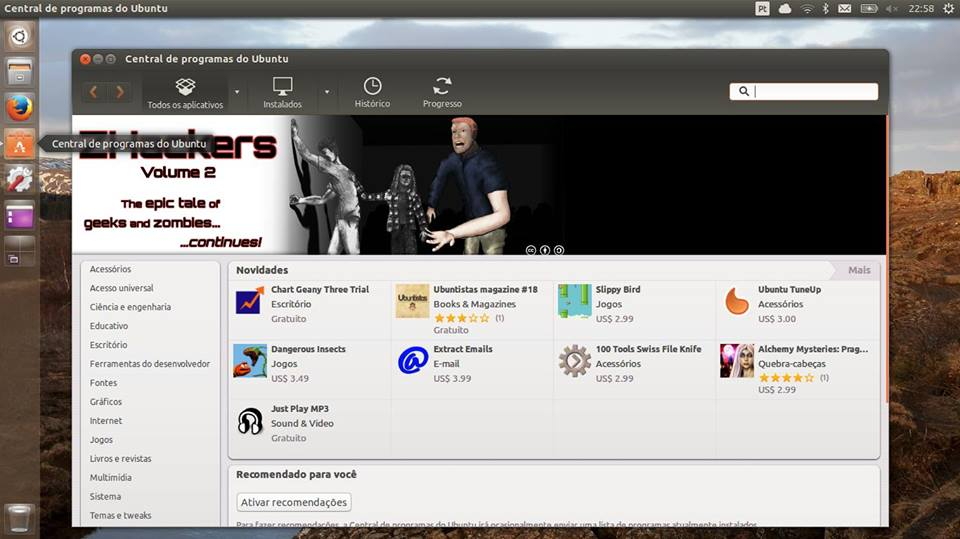
\includegraphics[scale=0.4]{linux5.png} 
\end{figure}
Resultado da procura do coq no gerenciador:\\
\begin{figure}[!htb]
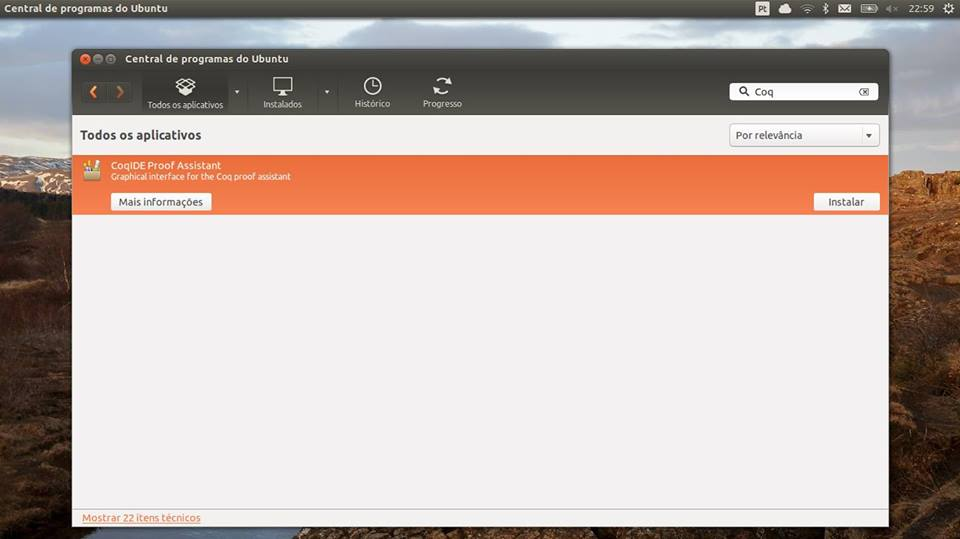
\includegraphics[scale=0.4]{linux2.png} 
\end{figure}
Informar o usu\'{a}rio mestre do linux, o q possui os privil\'{e}gios de instala\c{c}\~{a}o de programas.\\
\begin{figure}[!htb]
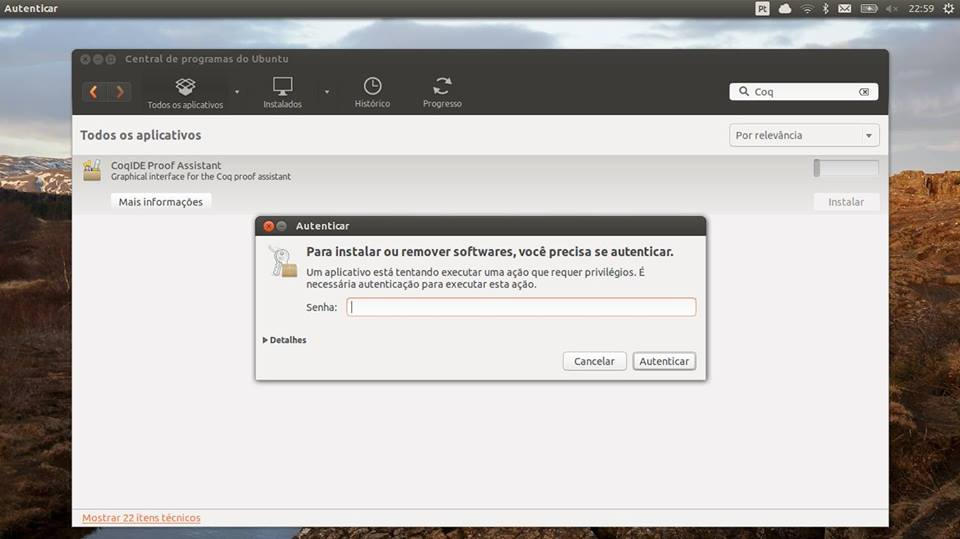
\includegraphics[scale=0.4]{linux1.png} 
\end{figure}
Indicativo que o programa foi instalado.\\
\begin{figure}[!htb]
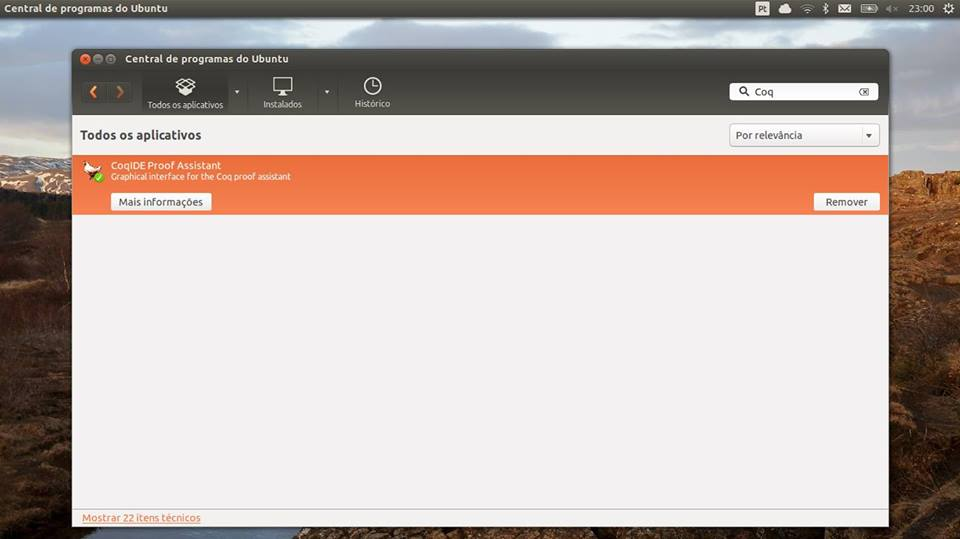
\includegraphics[scale=0.4]{linux3.png} 
\end{figure}
Depois de instalado o \'{i}cone do Coq aparece no painel.\\
\begin{figure}[!htb]
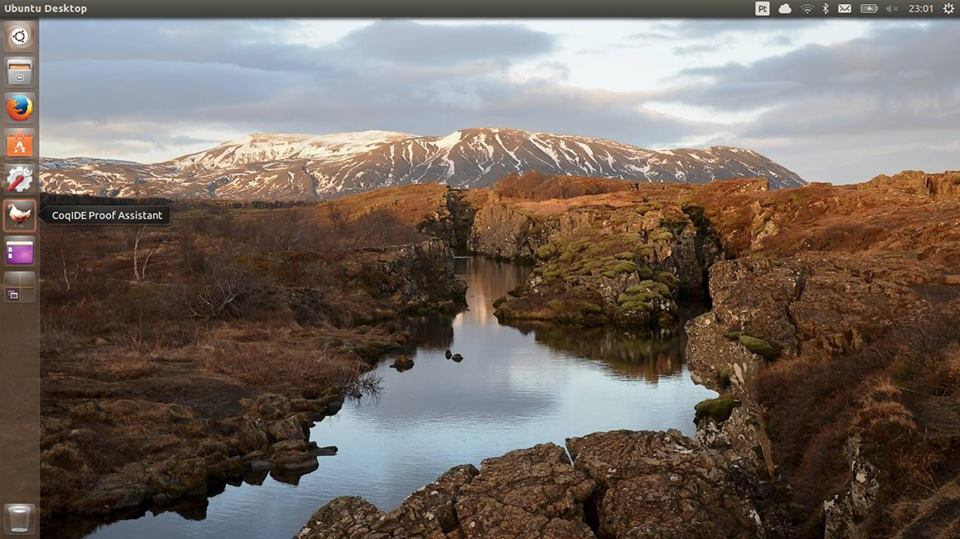
\includegraphics[scale=0.4]{linux6.png}
\end{figure}
Janela do Coq aberta:\\
\begin{figure}[!htb]
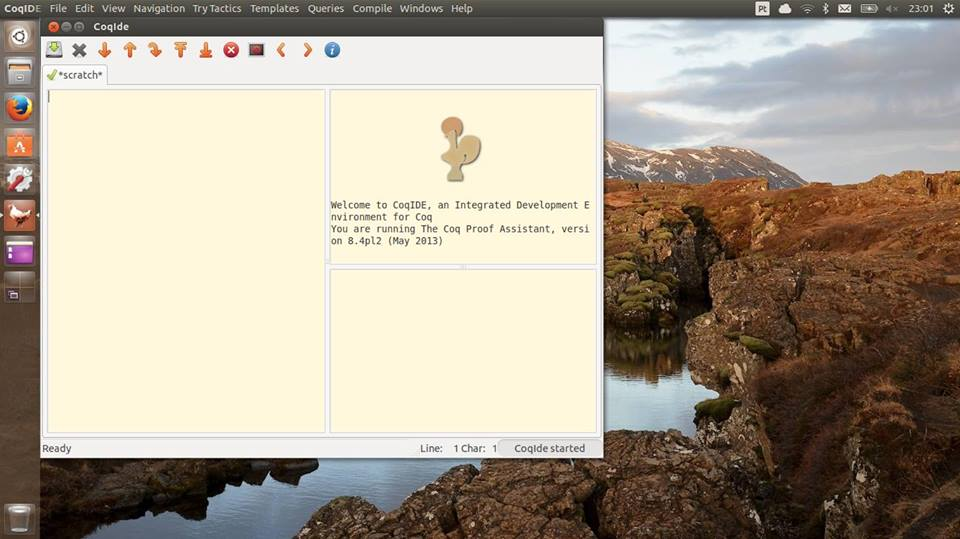
\includegraphics[scale=0.4]{linux4.png}
\end{figure}
\section{Instala\c{c}\~ao para MacOS}
}{}

\bibliographystyle{plain}
\bibliography{apostila}

\end{document}
